\documentclass[a4paper,twoside,openright,fleqn,11pt]{book}
\usepackage[T1]{fontenc}
\usepackage[light,slantedGreeks]{kpfonts}
\usepackage[utf8]{inputenc}
\usepackage[italian]{babel}

%%%%% Pacchetti caricati
\usepackage{layaureo}
\usepackage[autostyle=true]{csquotes}
\usepackage[style=numeric,hyperref,abbreviate=false,backend=bibtex]{biblatex}
\usepackage{fancyhdr,emptypage}
\usepackage{tensor} % per rappresentare i tensori
\usepackage[font=small,format=hang,labelfont=bf,textformat=period]{caption}
% per tabelle e figure
\usepackage{booktabs,longtable,graphicx,sidecap,subfig}
\usepackage{tikz,tikz-3dplot}
% `mathtools' serve per definire la norma e il valore assoluto
\usepackage{mathtools}
% pacchetti matematici dell'American Mathematical Society
\usepackage{amsthm}
% `bm' serve per scrivere i vettori in corsivo con il comando
% `\bm{vettore}'. Deve sostituire il comando `\mathbf{vettore}' perché questo
% restituisce erroneamente lettere in tondo, non in corsivo e non funziona con
% le lettere greche.
\usepackage{bm}
\usepackage[long,nodayofweek]{datetime}
\usepackage{makeidx}
\usepackage{siunitx}
\usepackage{hyperref}
%%%%% Fine pacchetti

%%%%% Impostazioni
%% testatine.
\pagestyle{fancy}
\fancyhf{} % svuota tutti i campi delle testatine e dei piedi
\setlength{\headheight}{14pt}
% Nella testatina (`head') a destra (`R') nelle pagine pari (`E') mettiamo il
% nome del capitolo (`\leftmark'), non tutto maiuscolo (`\nouppercase'). Sulla
% sinistra (`L') delle pagine dispari (`O') mettiamo il nome del paragrafo
% (`\rightmark').
\fancyhead[RE]{\slshape\footnotesize\nouppercase{\leftmark}}
\fancyhead[LO]{\slshape\footnotesize\nouppercase{\rightmark}}
% All'esterno di ogni pagina (cioè a sinistra (`L') nelle pagine pari (`E') e a
% destra (`R') nelle pagine dispari (`O')), nella testatina (`head') mettiamo il
% numero della pagina (`\thepage').
\fancyhead[LE,RO]{\thepage}

% impostazioni per il pacchetto `hyperref'. Per l'elenco di tutte le opzioni del
% documento consulta il manuale: `texdoc hyperref'
\hypersetup{
  pdftitle={Gravitazione e cosmologia},
  pdfauthor={Mosè Giordano},
  breaklinks=true,% permette di spezzare i link su più righe
  bookmarksnumbered,% inserisce i numeri delle sezioni nei segnalibri
  hidelinks % link neri e senza bordi colorati, adatto per la stampa
}

\sisetup{per-mode=symbol,
  inter-unit-product=\ensuremath{{}\cdot{}},
  exponent-product=\cdot,
  output-product=\cdot,
  separate-uncertainty=true,
  math-micro=\muup,
  text-micro=\ensuremath{\muup},
}

% Posiziona le didascalie sopra le tabelle
\captionsetup[table]{position=top}

\addbibresource{bibliografia.bib} % nome del file contenente la bibliografia
\defbibheading{bibliography}[\refname]{\chapter*{#1}\markboth{#1}{#1}}

\theoremstyle{plain}
\newtheorem*{teorema}{Teorema}

% librerie ti TikZ
\usetikzlibrary{calc,decorations.pathmorphing,decorations.pathreplacing,
  intersections,matrix,backgrounds}

% Stili per TikZ per rendere una matrix simile a una classica pmatrix di LaTeX.
% Vedi http://tex.stackexchange.com/a/26909
\tikzset{
  ams/.style={
    baseline=-.7ex,
    every left delimiter/.style={xshift=2pt},
    every right delimiter/.style={xshift=-2pt},
    every node/.style={inner sep=0pt},
  },
  ams matrix/.style={
    inner sep=1pt,
    column sep=1.5ex,
    row sep=2\arraycolsep,
    matrix of math nodes,
  },
  pmatrix/.style={
    ams,
    every matrix/.style={
      ams matrix,
      left delimiter={(},
      right delimiter={)},
    }
  }
}
%%%%% Fine impostazioni

%%%%% Comandi personalizzati
% ridefinisco i comandi per alcune lettere greche in modo che si usino le
% varianti
\renewcommand{\phi}{\varphi}
\renewcommand{\epsilon}{\varepsilon}

% Comando per indicare la variazione di una quantità.  Deve produrre una delta
% maiuscola diritta, visto che carico il pacchetto `kpfonts' con l'opzione
% `slantedGreeks' uso la macro `\Deltaup'.
\newcommand{\var}{\Deltaup}

% comando per evidenziare le sezioni da completare o espandere.  NOTA: è un
% comando provvisorio, serve solo durante la scrittura del testo, ricordarsi di
% eliminarlo quando non serve più.
\newcommand{\completare}[1]{\textcolor{red}{#1 (COMPLETARE)}}

% Operatori
\newcommand*{\dd}{\mathop{}\!\mathrm{d}} % Operatore differenziale \dd
\newcommand*{\cdd}{\mathop{}\!\mathrm{D}} % Differenziale covariante \cdd
\DeclareMathOperator{\e}{\mathrm{e}} % Numero di Eulero
\DeclareMathOperator{\diag}{diag}
\DeclareMathOperator{\uimm}{\mathrm{i}} % unità immaginaria
% Operatore valore assoluto \abs{x}. Usa \abs*{} per le frazioni
\DeclarePairedDelimiter{\abs}{\lvert}{\rvert}
% Operatore norma \norm{x}. Usa \norm*{} per le frazioni
\DeclarePairedDelimiter{\norm}{\lVert}{\rVert}

%% Derivate
% Derivata totale: \toder[ordine]{funzione}{variabile}
\newcommand*{\toder}[3][]{\frac{{\dd^{#1}}#2}{\dd {#3}^{#1}}}
% Derivata covariante: \covder[ordine]{tensore}{variabile}
\newcommand*{\covder}[3][]{\frac{{\cdd^{#1}}#2}{\dd {#3}^{#1}}}
% Derivata lungo una curva: \covder[ordine]{tensore}
\newcommand*{\curder}[2][]{\frac{{\cdd^{#1}}#2}{\cdd \tau^{#1}}}
% operatore d'alambertiano.  Definisco un comando specifico nel caso in cui si
% decidesse di cambiare la notazione (per esempio \Box invece di \Box^{2}).
\newcommand{\dalamb}{\Box^{2}}


% Derivata parziale \parder[ordine]{funzione}{variabile}
% Per la definizione del comando `parder' (per inserire le derivate parziali)
% vedi
% http://www.guitex.org/home/index.php?option=com_kunena&func=view&catid=5&id=42178&Itemid=60#42199
\makeatletter
\newcommand{\parder}[2]{\begingroup
  \@tempswafalse\toks@={}\count@=\z@
  \@for\next:=#2\do
    {\expandafter\check@var\next\@nil
     \advance\count@\parder@exp
     \if@tempswa
       \toks@=\expandafter{\the\toks@\,}%
     \else
       \@tempswatrue
     \fi
     \toks@=\expandafter{\the\expandafter\toks@\expandafter\partial\parder@var}}%
  \frac{\partial\ifnum\count@=\@ne\else^{\number\count@}\fi#1}{\the\toks@}%
  \endgroup}
\def\check@var{\@ifstar{\mult@var}{\one@var}}
\def\mult@var#1#2\@nil{\def\parder@var{#2^{#1}}\def\parder@exp{#1}}
\def\one@var#1\@nil{\def\parder@var{#1}\chardef\parder@exp\@ne}
\makeatother

% Derivate per le formule in linea (usare \frac in linea è eccessivo). La `l'
% iniziale nel nome distingue questi comandi da quelli per le formule fuori
% corpo. Non uso `\dd' ma `\mathrm{d}' perché nelle formule in linea `\dd'
% aggiunge una spaziatura non adatta. Non sono dei comandi bellissimi, ma
% permettono di passare facilmente da formula in linea a fuori corpo e viceversa
% cambiando una lettera.
% Derivata totale: \ltoder[ordine]{funzione}{variabile}
\newcommand*{\ltoder}[3][]{\mathrm{d}^{#1}#2 / \mathrm{d} {#3}^{#1}}
% Derivata parziale: \lparder[ordine]{funzione}{variabile}
\newcommand*{\lparder}[3][]{\partial^{#1} #2 / \partial {#3}^{#1}}
% NOTA: `\parder' e `\lparder' non sono completamente interscambiabili, il primo
% comando è molto più complesso e permette di inserire le derivate miste, a
% differenza del secondo.

% Versore. Esempi: versore x: `\versore{x}', versore i: \versor{\imath}, versore
% j: \versor{\jmath} (solo `i' e `j' richiedono `\imath' e `\jmath', altrimenti
% il puntino litiga con `\hat')
\newcommand*{\versor}[1]{\hat{\bm{#1}}}

% Ambiente per scrivere sistemi di equazioni.
% Vedi `L'arte di scrivere con LaTeX' di Pantieri.
% Esempio d'uso (in ambiente matematico):
%	\begin{sistema}
%         x+y+z=0 \\
%         2x-y=1 \\
%         y-4z=-3
%       \end{sistema}
\newenvironment{sistema}%
{\left\lbrace\begin{array}{@{}l@{}}}%
    {\end{array}\right.}

%% Campi notevoli
\let\numberset\mathbb
\newcommand{\N}{\numberset{N}}	% Naturali \N
\newcommand{\Z}{\numberset{Z}}	% Interi \Z
\newcommand{\R}{\numberset{R}}	% Reali \R
\newcommand{\C}{\numberset{C}}	% Complessi \C
\newcommand{\M}{\numberset{M}}	% spazio-tempo di Minkowski

% unità di misura aggiuntive (non-SI)
\DeclareSIUnit\dyne{dyn} % dyne
\DeclareSIUnit\erg{erg} % erg
\DeclareSIUnit\tonne{t} % tonnellata ("tonne" in inglese)
\DeclareSIUnit\parsec{pc} % parsec
\DeclareSIUnit\lightyear{ly} % anno luce
\DeclareSIUnit\radian{rad} % radiante
\DeclareSIUnit\solarmass{\ensuremath{M_{\odot}}} % massa solare
%%%%% Fine comandi personalizzati

\makeindex{}

\begin{document}
\frontmatter{}

%% copertina, rielaborazione dell'esempio `\titleGP' di pagina 34 del file di
%% documentazione `titlepages.pdf'
\thispagestyle{empty}
\begingroup
\scshape
\newdateformat{mydate}{\THEDAY{}~\monthname[\THEMONTH{}]~\THEYEAR{}}
\centering
\vspace*{\baselineskip}
\rule{\textwidth}{1.6pt}\vspace*{-\baselineskip}\vspace*{2pt}
\rule{\textwidth}{0.4pt}\\[\baselineskip]
{\LARGE Gravitazione\\ e \\[0.3\baselineskip]
  Cosmologia}\\[0.2\baselineskip]
\rule{\textwidth}{0.4pt}\vspace*{-\baselineskip}\vspace{3.2pt}
\rule{\textwidth}{1.6pt}\\[\baselineskip]
{\Large Appunti del corso tenuto dal professor Gabriele Ingrosso} \\
Lecce, a. a. 2011-2012\par
\vspace*{2\baselineskip}
Curato da \\[0.5\baselineskip]
Mosè Giordano\par
{\itshape Università del Salento\par}
\vfill

\includegraphics[width=2cm]{figure/logo_unisalento}\\
\mydate\today\par
\endgroup
%% Fine copertina

\cleardoublepage{}
\tableofcontents{} % indice generale
\cleardoublepage{}
\listoffigures{} % elenco delle figure

\cleardoublepage
\chapter{Convenzioni e notazioni usate}
\label{cha:notazioni}
\markboth{Convenzioni e notazioni usate}{Convenzioni e notazioni usate}

Nella teoria della relatività generale sono diffuse diverse notazioni e
convenzioni sui segni e i fattori numerici che compaiono in alcune formule.
Nella tabella~\ref{tab:notazione} è riportata la notazione adottata negli
appunti.  Gran parte dei presenti appunti si basano
su~\textcite{weinberg:gravitation}, quindi, se non diversamente specificato,
adotteremo le stesse convenzioni di questo testo.  Riportiamo di seguito in
dettagli le convenzioni scelte.

Con le lettere greche ($\alpha,\beta,\dots,\mu,\nu,\dots$) rappresenteremo
indici che possono assumere i valori $0$, $1$, $2$ e $3$, mentre con le lettere
latine ($a,b,\dots,i,j,\dots$) indici che assumono i valori $1$, $2$, $3$.  Si
noti che \textcite{landau:campi} seguono la convenzione opposta: gli indici
latini assumono i valori $0$, $1$, $2$ e $3$, gli indici greci $1$, $2$ e $3$.

Dove non chiaramente dichiarato il contrario, adottiamo, come è di consuetudine
all'interno della relatività, la \index{convenzione!di Einstein per la somma}
\emph{convenzione di Einstein per la somma}: se in un termine un indice compare
due volte, di cui una volta controvariante (sopra) e una volta covariante
(sotto), esso è chiamato \index{indice!muto}\emph{muto} (o \emph{contratto}), si
sottintende una somma sui possibili valori che l'indice può assumere e si omette
il simbolo di sommatoria.  Gli indici non muti sono chiamati
\index{indice!libero}\emph{liberi}.  In un'identità fra tensori gli indici
liberi devono comparire in ugual numero e nelle stesse posizioni (superiormente
o inferiormente) in ambo i membri.  Sebbene possa succedere che, casualmente, in
un certo sistema di riferimento le componenti controvarianti di un tensore $A$
siano uguali alle componenti covarianti di un altro tensore $B$
\begin{equation}
  \tensor{A}{^{\alpha}_{\beta}^{\gamma}} = B^{\alpha\beta\gamma},
\end{equation}
questo non è valido in un altro sistema di riferimento e l'equazione precedente
non è, quindi, legittima.  Si noti inoltre che questa non è corretta dal punto
di vista tensoriale poiché l'indice libero $\beta$ è in un membro controvariante
e nell'altro covariante.  L'espressione
$A^{\mu\sigma}B_{\mu} = A^{0\sigma}B_{0} + A^{i\sigma}B_{i}$, scritta
utilizzando la convenzione di Einstein, equivale, esplicitando la sommatoria, a
\begin{equation}
  \sum_{\mu=0}^{3} A^{\mu\sigma}B_{\mu} = A^{0\sigma}B_{0} + \sum_{i=1}^{3}
  A^{i\sigma}B_{i} = A^{0\sigma}B_{0} + A^{1\sigma}B_{1} + A^{2\sigma}B_{2} +
  A^{3\sigma}B_{3},
\end{equation}
in cui gli indici $\mu$ e $i$ sono muti e $\sigma$ è libero.  Gli indici muti
sono così denominati poiché non compaiono nell'espressione esplicita.  Gli
indici muti possono essere rinominati a patto di non utilizzare indici muti già
utilizzati in quel termine oppure indici liberi, però una coppia di indici muti
può essere scambiata con un'altra coppia di indici muti.  Quindi l'espressione
$\tensor{T}{^{\alpha\beta\gamma}_{\alpha\gamma}}$ può essere anche scritta come
$\tensor{T}{^{\mu\beta\nu}_{\mu\nu}}$ oppure
$\tensor{T}{^{\gamma\beta\alpha}_{\gamma\alpha}}$ ma \emph{non} come
$\tensor{T}{^{\beta\beta\gamma}_{\beta\gamma}}$ oppure
$\tensor{T}{^{\alpha\beta\alpha}_{\alpha\alpha}}$.

La velocità della luce nel vuoto $c = \SI{299792458}{\metre\per\second}$ è posta
uguale a $1$.  Di conseguenza tutte le velocità sono adimensionali (in
particolare sono espresse in unità di $c$), lunghezze e tempo hanno la stessa
dimensione.  Per ristabilire la coerenza dimensionale delle equazioni bisogna
utilizzare l'adeguato numero di potenze di $c$.

Alcuni fondamentali tensori della relatività generale vengono definiti dai
diversi autori adottando diverse scelte di segni.  In particolare i tensori in
questione sono
\begin{subequations}
  \label{eq:convenzione-segni}
  \begin{align}
    \eta_{\mu\nu} &= S_{1} \cdot \diag(-1,+1,+1,+1), \\
    \tensor{R}{^{\lambda}_{\mu\nu\kappa}} &= S_{2} \cdot
    (\tensor{\Gamma}{^{\lambda}_{\mu\kappa,\nu}} -
    \tensor{\Gamma}{^{\lambda}_{\mu\nu,\kappa}} +
    \tensor{\Gamma}{^{\eta}_{\mu\kappa}} \tensor{\Gamma}{^{\lambda}_{\eta\nu}} -
    \tensor{\Gamma}{^{\eta}_{\mu\nu}}
    \tensor{\Gamma}{^{\lambda}_{\eta\kappa}}), \\
    G_{\mu\nu} &= S_{3} \cdot \frac{8\pi G}{c^{4}} T_{\mu\nu}, \\
    R_{\mu\kappa} &= S_{2} \cdot S_{3} \cdot
    \tensor{R}{^{\lambda}_{\mu\lambda\kappa}},
  \end{align}
\end{subequations}
in cui $\eta_{\mu\nu}$ è il tensore metrico di Minkowski,
$\tensor{R}{^{\lambda}_{\mu\nu\kappa}}$ è il tensore di Riemann, $R_{\mu\kappa}$
è il tensore di Ricci e $G_{\mu\nu}$ è il tensore di Einstein e $S_{1}$,
$S_{2}$, $S_{3}$ sono i segni che possono essere scelti uguali a $+$ oppure $-$.
In questi appunti seguiamo la stessa convenzione di
\textcite{weinberg:gravitation} ovvero $(S_{1}, S_{2}, S_{3}) = (+--)$.  I testi
\textcites{barone:relativita,landau:campi} adottano la convenzione $(-++)$,
\textcite{misner:gravitation} seguono la convenzione $(+++)$, mentre
\textcite{ohanian:gravitazione} hanno scelto la convenzione $(-+-)$.

\begin{longtable}{c
    p{.40\textwidth}
    p{.23\textwidth}}
  % intestazione iniziale
  \caption{Notazione usata in questi appunti}
  \label{tab:notazione} \\
  \toprule
  Simbolo & Significato & Riferimento \\
  \midrule
  \endfirsthead
  % intestazione normale
  \multicolumn{3}{l}{\footnotesize\itshape
    Continua dalla pagina precedente} \\
  \toprule
  Simbolo & Significato & Riferimento \\
  \midrule
  \endhead
  % piede normale
  \midrule \multicolumn{3}{r}{\footnotesize\itshape
    Continua nella prossima pagina} \\
  \endfoot
  % piede finale
  \bottomrule \multicolumn{3}{r}{\footnotesize\itshape
    Si conclude dalla pagina precedente} \\
  \endlastfoot
  % inizio corpo della tabella
  $\e = \lim_{n} (1+1/n)^{n}$ & Numero di Eulero o di Nepero. & \\[1.6ex]
  $\uimm = \sqrt{-1}$ & Unità immaginaria. & \\[1.6ex]
  $\Re \{z\}$ & Parte reale del numero complesso $z$. & \\
  % $\Im \{z\}$ & Parte immaginaria del numero complesso $z$. & \\
  $\abs{z}$ & Modulo del numero $z$.  & \\
  $\mathcal{O}$ & O-grande. & \\
  $\bm{A} = (A^{1}, A^{2}, A^{3})$ & Vettore tridimensionale con componenti
  $A^{1}$, $A^2$ e $A^{3}$. & \\
  $\norm{\bm{A}}$ & Norma del
  vettore $\bm{A}$. & \\
  $A^{\mu} = (A^{0}, \bm{A})$ & Quadrivettore controvariante con componente
  temporale $A^{0}$ e componenti spaziali $\bm{A}$. &
  Paragrafo~\ref{sec:calcolo-tensoriale-minkowski} e
  capitolo~\ref{cha:calcolo-tensoriale}. \\
  $A_{\mu} = (A_{0}, \bm{A})$ & Quadrivettore covariante con componente
  temporale $A_{0}$ e componenti spaziali $\bm{A}$. &
  Paragrafo~\ref{sec:calcolo-tensoriale-minkowski} e
  capitolo~\ref{cha:calcolo-tensoriale}. \\
  $\tensor*{T}{^{\alpha_{1}\dots\alpha_{p}}_{\beta_{1}\dots\beta_{q}}}$ &
  Quadritensore. & Paragrafo~\ref{sec:calcolo-tensoriale-minkowski} e
  capitolo~\ref{cha:calcolo-tensoriale}. \\
  $\dd \tau^{2} = \dd t^{2} - \dd \bm{x}^{2}$ & Metrica nello spazio di
  Minkowski. & Paragrafo~\ref{sec:trasformazioni-lorentz}. \\
  $\eta_{\alpha\beta}$ & Tensore metrico di Minkowski. &
  Paragrafo~\ref{sec:trasformazioni-lorentz}. \\
  $\tensor{\delta}{^{\alpha}_{\beta}}$ & Delta di Kronecker quadrimensionale. &
  Paragrafo~\ref{sec:trasformazioni-lorentz}. \\
  $\tensor{\Lambda}{^{\alpha}_{\beta}}$ & Matrice di Lorentz. &
  Paragrafo~\ref{sec:trasformazioni-lorentz}. \\
  $\gamma_{v} = \dfrac{1}{\sqrt{1-v^{2}}}$ & Fattore di Lorentz associato al
  boost $v$. & Paragrafo~\ref{sec:trasformazioni-lorentz}. \\
  $\partial_{\mu} A_{\nu} = A_{\nu,\mu} =
  \displaystyle\parder{A_{\nu}}{x^{\mu}}$
  & Derivata ordinaria di $A_{\nu}$ rispetto alla coordinata $x^{\mu}$. &
  Paragrafo~\ref{sec:derivazione-minkowski}. \\
  $\partial^{\mu} A_{\nu} = \tensor{A}{_{\nu}^{,\mu}} =
  \displaystyle\parder{A_{\nu}}{x_{\mu}}$
  & Derivata ordinaria di $A_{\nu}$ rispetto alla coordinata $x_{\mu}$. &
  Paragrafo~\ref{sec:derivazione-minkowski}. \\
  $ \dalamb = \partial^{\alpha}\partial_{\alpha}$ & Operatore d'Alambertiano. &
  Paragrafo~\ref{sec:derivazione-minkowski}. \\
  $\epsilon^{\alpha\beta\gamma\delta}$ & Tensore di Levi-Civita &
  Paragrafo~\ref{sec:tensore-levi-civita}. \\
  $\dd^{4} x = \dd x^{0}\dd x^{1}\dd x^{2}\dd x^{3}$ & Elemento infinitesimo di
  volume quadrimensionale. & \\
  $\dd \Sigma_{\mu}$ & Elemento infinitesimo di ipersuperficie
  tridimensionale. & Appendice~\ref{cha:teorema-gauss}. \\
  $\dd^{3} \bm{x} = \dd V$ & Elemento infinitesimo di volume tridimensionale. &
  \\
  $F^{\alpha\beta}$ & Tensore del campo elettromagnetico. &
  Paragrafo~\ref{sec:equazioni-maxwell}. \\
  $S = \displaystyle\int \Lambda \dd^{4} x$ & Azione associata alla densità di
  lagrangiana $\Lambda$. & Paragrafo~\ref{sec:tensore-energia-impulso}. \\
  $\tensor{T}{^{\beta}_{\alpha}}$ & Tensore energia-impulso. &
  Paragrafo~\ref{sec:tensore-energia-impulso}. \\[1.6ex]
  $\tensor{\Gamma}{^{\lambda}_{\mu\nu}}$ & Connessione affine. &
  Paragrafi~\ref{sec:equazione-moto}, \ref{sec:relazione-g-Gamma} e
  \ref{sec:derivazione-covariante}. \\
  $g_{\mu\nu}$ & Tensore metrico nella relatività generale. &
  Paragrafi~\ref{sec:equazione-moto}, \ref{sec:relazione-g-Gamma} e
  \ref{sec:tensore-metrico}. \\
  $r_{\textup{S}}$ & Raggio di Schwarzschild. &
  Paragrafo~\ref{sec:limite-newtoniano}. \\[1.6ex]
  $g = -\det(g_{\mu\nu})$ & Opposto del determinante del tensore metrico. &
  Paragrafo~\ref{sec:tensore-metrico}. \\
  $V_{\mu;\nu} = \displaystyle\covder{V_{\mu}}{x^{\nu}}$ & Derivata covariante
  di $V_{\mu}$ rispetto alla coordinata $x^{\nu}$. &
  Paragrafo~\ref{sec:derivazione-covariante}. \\
  $\cdd V_{\mu}$ & Differenziale covariante di $V_{\mu}$. &
  Paragrafo~\ref{sec:differenziale-covariante}. \\[1.6ex]
  $\displaystyle\curder{V_{\mu}}$ & Derivata di $V_{\mu}$ lungo una curva
  parametrizzata da $\tau$. & Paragrafo~\ref{sec:differenziale-covariante}. \\
  $\tensor{R}{^{\lambda}_{\mu\nu\kappa}}$ & Tensore di curvatura di
  Riemann-Christoffel. & Paragrafo~\ref{sec:tensore-riemann}. \\
  $R_{\mu\kappa} = \tensor{R}{^{\lambda}_{\mu\lambda\kappa}}$ & Tensore di
  Ricci. & Paragrafo~\ref{sec:tensore-riemann}. \\[1.6ex]
  $R = \tensor{R}{^{\mu}_{\mu}}$ & Curvatura scalare. &
  Paragrafo~\ref{sec:tensore-riemann}. \\[1.6ex]
  $G^{\mu\nu} = R^{\mu\nu} - \dfrac{1}{2} g^{\mu\nu}R$ & Tensore di Einstein. &
  Paragrafo~\ref{sec:identita-bianchi}. \\[1.6ex]
  $M_{\odot} = \SI{2e33}{\gram}$ & Massa solare. & \\
\end{longtable}


%%% Local Variables:
%%% mode: latex
%%% TeX-master: "../gravitazione"
%%% fill-column: 80
%%% TeX-PDF-mode: t
%%% End:


\cleardoublepage{}
\mainmatter{}
\cleardoublepage
\chapter{Richiami di relatività speciale}
\label{cha:relativita-speciale}

\section{Trasformazioni di Lorentz}
\label{sec:trasformazioni-lorentz}

La relatività speciale, o ristretta, si basa su due postulati:
\begin{enumerate}
\item\emph{tutte le leggi fisiche assumono la stessa forma in qualsiasi sistema
    di riferimento inerziale (\index{principio!di relatività}principio di
    relatività)};
\item \emph{la velocità della luce nel vuoto ha lo stesso valore in tutti i
    sistemi di riferimento inerziali (costanza della velocità della luce)}.
\end{enumerate}

L'ambiente in cui si svolgono i fenomeni fisici descritti dalla relatività
speciale è uno spazio quadrimensionale piatto, composto da una coordinata
temporale e tre spaziali, chiamato \index{spazio!di Minkowski}
\emph{spazio di Minkowski} e che indicheremo con il simbolo $\M$.  Un elemento
dello spazio di Minkowski è chiamato \index{evento}\emph{evento}.  Lo spazio di
Minkowski si distingue dal corrispondente spazio euclideo quadrimensionale
$\R^{4}$ e anche dallo spazio ordinario tridimensionale $\R^{3}$ in quanto
utilizza una metrica differente da quelle usualmente adottate in $\R^{3}$ ed
$\R^{4}$.

Nello spazio ordinario $\R^{3}$ si definisce la metrica, ovvero la distanza fra
due punti infinitesimamente vicini di coordinate cartesiane
$\bm{x} = (x,y,z) \equiv (x_{1},x_{2},x_{3})$ e
$\bm{x} + \dd \bm{x} = (x+\dd x,y+\dd y,z+\dd z) \equiv (x_{1}+\dd
x_{1},x_{2}+\dd x_{2},x_{3}+\dd x_{3})$ come
\begin{equation}
  \dd\bm{x}^{2} = (\dd x_{1})^{2} + (\dd x_{2})^{2} + (\dd x_{3})^{2} =
  \sum_{i=1}^{3} \sum_{j=1}^{3} \delta_{ij} \dd x_{i} \dd x_{j},
\end{equation}
dove $\delta_{ij}$ è il tensore metrico dato da
\begin{equation}
  \delta_{ij} = \diag (+1,+1,+1) =
  \begin{pmatrix}
    +1 & 0  & 0  \\
    0  & +1 & 0  \\
    0  & 0  & +1
  \end{pmatrix}.
\end{equation}
Allo stesso modo, nello spazio $\R^{4}$ si utilizza il tensore metrico
rappresentato da $\diag (+1,+1,+1,+1)$.  Una generica trasformazione lineare
omogenea delle coordinate cartesiane $(x,y,z) \equiv (x_{1},x_{2},x_{3})$ che
lasci invariate la metrica, cioè che soddisfi la condizione
$\dd\bm{x}^{2} = \dd\bm{x}'^{2}$, può essere scritta come
\begin{equation}
  x'_{i} = \sum_{j=1}^{3} R_{ij}x_{j}, \qquad i,j = 1,2,3,
\end{equation}
con $R_{ij}$ costanti reali, e la matrice di componenti $R_{ij}$ è una matrice
di rotazione.

Nello spaziotempo di Minkowski definiamo le
\index{coordinata!controvariante}\emph{coordinate controvarianti} di un evento
che avviene al tempo $t$ nel punto $\bm{x}$ dello spazio tridimensionale con
coordinate cartesiane $(x,y,z) \equiv (x^{1}, x^{2}, x^{3})$ come
\begin{equation}
  \label{eq:coord-controvariante}
  x^{\alpha} = (x^{0},x^{i}) = (t, \bm{x}),
\end{equation}
con $\alpha$ che varia fra $0$, $1$, $2$ e $3$ e $i$ fra $1$, $2$ e $3$.  La
\index{metrica!nello spazio di Minkowski}\emph{metrica} è data da
\begin{equation}
  \dd \tau^{2} = \dd t^{2} - \dd \bm{x}^{2} = -\tensor{\eta}{_{\alpha\beta}}\dd
  x^{\alpha} \dd x^{\beta},
\end{equation}
in cui $\tensor{\eta}{_{\alpha\beta}}$ è il
\index{tensore!metrico di Minkowski}\emph{tensore metrico covariante di
  Minkowski}
\begin{equation}
  \label{eq:tensore-metrico-controvariante}
  \tensor{\eta}{_{\alpha\beta}} =
  \begin{pmatrix}
   \eta_{00} & \eta_{01} & \eta_{02} & \eta_{03} \\
   \eta_{10} & \eta_{11} & \eta_{12} & \eta_{13} \\
   \eta_{20} & \eta_{21} & \eta_{22} & \eta_{23} \\
   \eta_{30} & \eta_{31} & \eta_{32} & \eta_{33}
  \end{pmatrix}
  =
  \begin{pmatrix}
    -1 & 0  & 0  & 0 \\
    0  & +1 & 0  & 0 \\
    0  & 0  & +1 & 0 \\
    0  & 0  & 0  & +1
  \end{pmatrix}.
\end{equation}
Se si scelgono coordinate spaziali non cartesiane, come per esempio le
coordinate sferiche o cilindriche, il tensore metrico assume una forma
differente.  Se non diversamente specificato useremo sempre coordinate spaziali
cartesiane.  Questo tensore definisce una metrica pseudo euclidea con segnatura
$(-+++)$,\footnote{Nelle presenti note abbiamo adottato questa segnatura, ma non
  è l'unica possibile nello spazio di Minkowski.  Un'altra segnatura largamente
  usata è $(+---)$.}
invece in $\R^{4}$ abbiamo visto che si utilizza la segnatura $(++++)$.  Una
\index{trasformazione!di Lorentz}\emph{trasformazione di Lorentz} non omogenea è
una trasformazione lineare nello spazio di Minkowski da un sistema di
riferimento inerziale di coordinate $x^{\alpha}$ a un altro sistema di
riferimento inerziale di coordinate
\begin{equation}
  \label{eq:trasformazione-lineare}
  x'^{\alpha} = \tensor{\Lambda}{^{\alpha}_{\beta}}x^{\beta} + a^{\alpha},
\end{equation}
con $\tensor{\Lambda}{^{\alpha}_{\beta}}$ e $a^{\alpha}$ costanti, che mantenga
invariata la distanza fra due eventi, cioè la metrica
$\dd\tau^{2} = -\eta_{\alpha\beta}\dd x^{\alpha}\dd x^{\beta}$ in $\M$.
Richiediamo che la trasformazione $x^{\alpha} \to x'^{\alpha}$ sia lineare per
rispettare la condizione di omogeneità dello spazio (la lunghezza di una sbarra
non deve dipendere dalla posizione degli estremi), del tempo (la lunghezza della
sbarra non deve dipendere dall'istante di tempo in cui la misuriamo) e di
isotropia dello spazio (la lunghezza della sbarra non deve dipendere neanche
dalla direzione in cui la guardiamo).  In questo modo un moto rettilineo
uniforme in un sistema di riferimento inerziale è ancora un moto rettilineo
uniforme anche nell'altro sistema di riferimento inerziale.  L'importanza delle
trasformazioni di Lorentz risiede nel fatto che una trasformazione fra due
sistemi di riferimento che sia coerente con i postulati della relatività
ristretta deve essere tale da lasciare invariata la
metrica.\footnote{Per una dimostrazione di questa proprietà
  vedi~\textcite[34-37]{barone:relativita}.}
I differenziali delle coordinate nel nuovo sistema si ricavano
dalla~\eqref{eq:trasformazione-lineare}
\begin{equation}
  \label{eq:trasformazione-differenziali}
  \dd x'^{\alpha} = \tensor{\Lambda}{^{\alpha}_{\beta}}\dd x^{\beta}.
\end{equation}
Dall'equazione precedente abbiamo inoltre
\begin{equation}
  \tensor{\Lambda}{^{\alpha}_{\beta}} = \parder{x'^{\alpha}}{x^{\beta}}.
\end{equation}

Affinché una trasformazione lineare~\eqref{eq:trasformazione-lineare} delle
coordinate sia di Lorentz, cioè affinché conservi la metrica, deve valere
\begin{equation}
  \begin{split}
    \dd \tau'^{2} &= -\tensor{\eta}{_{\alpha\beta}}\dd x'^{\alpha}\dd x'^{\beta}
    = -\tensor{\eta}{_{\alpha\beta}} \tensor{\Lambda}{^{\alpha}_{\gamma}} \dd
    x^{\gamma} \tensor{\Lambda}{^{\beta}_{\delta}} \dd x^{\delta} \\
    &= \dd \tau^{2} = -\tensor{\eta}{_{\gamma\delta}} \dd x^{\gamma} \dd x^{\delta},
  \end{split}
\end{equation}
da cui, confrontando terzo e quinto membro, otteniamo la relazione fondamentale
del tensore metrico
\begin{equation}
  \label{eq:rel-fond-tensore-metrico}
  \tensor{\eta}{_{\alpha\beta}} \tensor{\Lambda}{^{\alpha}_{\gamma}}
  \tensor{\Lambda}{^{\beta}_{\delta}} = \tensor{\eta}{_{\gamma\delta}}.
\end{equation}
Questa relazione impone $10$ condizioni indipendenti in quanto il tensore
metrico $\tensor{\eta}{_{\gamma\delta}}$ è simmetrico quindi solo $10$ delle sue
$16$ componenti sono indipendenti.

Ciascuna trasformazione di Lorentz è rappresentabile con una specifica
\emph{matrice di Lorentz} $\Lambda$, di dimensione $4 \times 4$, i cui elementi
sono le $\tensor{\Lambda}{^{\alpha}_{\beta}}$
\begin{equation}
  \Lambda =
  \begin{pmatrix}
    \tensor{\Lambda}{^{0}_{0}} & \tensor{\Lambda}{^{0}_{1}} &
    \tensor{\Lambda}{^{0}_{2}} & \tensor{\Lambda}{^{0}_{3}} \\
    \tensor{\Lambda}{^{1}_{0}} & \tensor{\Lambda}{^{1}_{1}} &
    \tensor{\Lambda}{^{1}_{2}} & \tensor{\Lambda}{^{1}_{3}} \\
    \tensor{\Lambda}{^{2}_{0}} & \tensor{\Lambda}{^{2}_{1}} &
    \tensor{\Lambda}{^{2}_{2}} & \tensor{\Lambda}{^{2}_{3}} \\
    \tensor{\Lambda}{^{3}_{0}} & \tensor{\Lambda}{^{3}_{1}} &
    \tensor{\Lambda}{^{3}_{2}} & \tensor{\Lambda}{^{3}_{3}}
  \end{pmatrix}.
\end{equation}
Possiamo scrivere la~\eqref{eq:rel-fond-tensore-metrico} nella seguente forma
matriciale
\begin{equation}
  \Lambda^{\textup{T}}\eta\Lambda = \eta
\end{equation}
dalla quale abbiamo
\begin{equation}
  \det\eta = \det(\Lambda^{\textup{T}}\eta\Lambda) = \det\eta
  \det(\Lambda^{\textup{T}}\Lambda) = \det\eta (\det\Lambda)^{2}
\end{equation}
e quindi deve valere la condizione
\begin{equation}
  \det\Lambda = \pm 1.
\end{equation}
Le trasformazioni di Lorentz con $\det\Lambda = +1$ sono chiamate
\emph{proprie}, quelle con $\det\Lambda = -1$ sono chiamate \emph{improprie}.

\begin{figure}
  \centering
  \tdplotsetmaincoords{70}{100}
  \begin{tikzpicture}[tdplot_main_coords,font=\footnotesize,scale=3]
    \node[shape=coordinate] (O1) at (0,0,0) [label=above right:$O$] {};
    \node[shape=coordinate] (O2) at (-1,0.5,0.3) [label=above right:$O'$] {};
    \draw[->] (O1) -- ++(1,0,0) node[anchor=north east] {$x$}; % asse x
    \draw[->] (O1) -- ++(0,1,0) node[anchor=north west] {$y$}; % asse y
    \draw[->] (O1) -- ++(0,0,1) node[anchor=south] (Z1) {$z$}; % asse z
    \node at (Z1) [label=below right:$\mathcal{S}$] {};% sistema di riferimento
    \draw[->] (O2) -- ++(1,0,0) node[anchor=north east] {$x'$}; % asse x'
    \draw[->] (O2) -- ++(0,1,0) node[anchor=north west] {$y'$}; % asse y'
    \draw[->] (O2) -- ++(0,0,1) node[anchor=south] (Z2) {$z'$}; % asse z'
    \node at (Z2) [label=below right:$\mathcal{S}'$] {};% sistema di riferimento
    \draw[->,thick] (O1) -- node[above] {$\bm{v}$} ++(0.3,-0.4,0.3); % velocità
  \end{tikzpicture}
  \caption[Sistemi di riferimento inerziali in moto l'uno rispetto
  all'altro]{Sistemi di riferimento inerziali, con gli assi corrispondenti
    paralleli, in moto l'uno rispetto all'altro}
  \label{fig:trasformazioni-lorentz}
\end{figure}
Vediamo come si trasformano le coordinate $x^{\alpha}$ di un evento in un
sistema di riferimento per effetto di una \emph{trasformazione di velocità}, o
\index{boost}\emph{boost}, vale a dire una trasformazione tra due sistemi di
riferimento inerziali con gli assi cartesiani corrispondenti paralleli e in moto
l'uno rispetto all'altro con velocità costante $\bm{v}$.  Vogliamo quindi
determinare la forma esplicita della matrice di Lorentz per il caso particolare
di un boost.  Consideriamo una particella a riposo in un sistema di riferimento
$\mathcal{S}$ che si muove con velocità $\bm{v} = (v_{1},v_{2},v_{3})$ rispetto
a un altro sistema di riferimento inerziale $\mathcal{S}'$, come nella
figura~\ref{fig:trasformazioni-lorentz}.\footnote{Si noti che il sistema di
  riferimento $\mathcal{S}$ vede il sistema $\mathcal{S}'$ muoversi con velocità
  $-\bm{v}$.  Numerosi autori considerano il sistema di riferimento
  $\mathcal{S}'$ in moto rispetto al sistema $\mathcal{S}$ con velocità
  $\bm{v}$, questo comporterà una differenza di segno in numerose equazioni
  rispetto a quelle ricavate da questi autori.}
Poiché nel sistema $\mathcal{S}$ per la particella risulta $\dd\bm{x} = \bm{0}$,
si ricava
\begin{subequations}
  \begin{align}
    \dd x'^{i} &= \tensor{\Lambda}{^{i}_{\alpha}}\dd x^{\alpha} =
    \tensor{\Lambda}{^{i}_{0}}\dd x^{0} + \tensor{\Lambda}{^{i}_{j}}\dd x^{j} =
    \tensor{\Lambda}{^{i}_{0}}\dd t \\
    \dd x'^{0} &= \tensor{\Lambda}{^{0}_{\alpha}}\dd x^{\alpha} =
    \tensor{\Lambda}{^{0}_{0}}\dd x^{0} + \tensor{\Lambda}{^{0}_{j}}\dd x^{j} =
    \tensor{\Lambda}{^{0}_{0}}\dd t.
  \end{align}
\end{subequations}
Dividendo membro a membro abbiamo
\begin{equation}
  \toder{x'^{i}}{x'^{0}} = \toder{x'^{i}}{t'} = v_{i} =
  \frac{\tensor{\Lambda}{^{i}_{0}}}{\tensor{\Lambda}{^{0}_{0}}},
\end{equation}
in quanto $\ltoder{x'^{i}}{t'}$ è la componente $v_{i}$ della velocità della
particella vista dal sistema $\mathcal{S}'$.  Allora
\begin{equation}
  \tensor{\Lambda}{^{i}_{0}} = v_{i}\tensor{\Lambda}{^{0}_{0}}.
\end{equation}
Ponendo $\gamma = \delta = 0$ nella~\eqref{eq:rel-fond-tensore-metrico} risulta
\begin{equation}
  \begin{split}
    -1 &= \tensor{\eta}{_{00}} = \tensor{\eta}{_{\alpha\beta}}
    \tensor{\Lambda}{^{\alpha}_{0}} \tensor{\Lambda}{^{\beta}_{0}} =
    \tensor{\eta}{_{00}}(\tensor{\Lambda}{^{0}_{0}})^{2} + \tensor{\eta}{_{ij}}
    \tensor{\Lambda}{^{i}_{0}} \tensor{\Lambda}{^{j}_{0}}
    \\
    &= -(\tensor{\Lambda}{^{0}_{0}})^{2} + \delta_{ij}
    \tensor{\Lambda}{^{i}_{0}} \tensor{\Lambda}{^{j}_{0}} =
    -(\tensor{\Lambda}{^{0}_{0}})^{2}+\sum_{i}(\tensor{\Lambda}{^{i}_{0}})^{2},
  \end{split}
\end{equation}
quindi
\begin{equation}
  (\tensor{\Lambda}{^{0}_{0}})^{2} = 1 +
  \sum_{i}(\tensor{\Lambda}{^{i}_{0}})^{2} \geq 1,
\end{equation}
cioè per ogni trasformazione di Lorentz deve aversi
\begin{equation}
  \tensor{\Lambda}{^{0}_{0}} \geq 1 \text{ oppure } \tensor{\Lambda}{^{0}_{0}}
  \leq -1.
\end{equation}
Le trasformazioni con $\tensor{\Lambda}{^{0}_{0}} \geq +1$ sono chiamate
\emph{ortocrone}, quelle con $\tensor{\Lambda}{^{0}_{0}} \leq -1$
\emph{anticrone}.  Le trasformazioni di Lorentz proprie e ortocrone sono dette
\emph{trasformazioni di Lorentz ristrette} o \emph{speciali}.  Richiedendo che
il boost sia una trasformazione ristretta abbiamo
\begin{equation}
  \tensor{\Lambda}{^{0}_{0}} = \frac{1}{\sqrt{1-\sum_{i}(v_{i})^{2}}} =
  \frac{1}{\sqrt{1-v^{2}}} = \gamma(v) \equiv \gamma,
\end{equation}
con $v^{2} = \sum_{i}(v_{i})^{2}$ modulo quadro del vettore $\bm{v}$.
$\gamma(v)$ è chiamato \index{fattore!di Lorentz}\emph{fattore di Lorentz}
associato al boost $v$.  Quindi risulta anche
\begin{equation}
  \tensor{\Lambda}{^{i}_{0}} = v_{i}\tensor{\Lambda}{^{0}_{0}} = v_{i}\gamma.
\end{equation}
Le altre componenti $\tensor{\Lambda}{^{\alpha}_{\beta}}$ non sono univocamente
determinate.  Una scelta conveniente che permette di soddisfare
la relazione fondamentale~\eqref{eq:rel-fond-tensore-metrico} è
\begin{subequations}
  \begin{align}
    \tensor{\Lambda}{^{0}_{i}} &= \tensor{\Lambda}{^{i}_{0}} = v_{i}\gamma, \\
    \tensor{\Lambda}{^{i}_{j}} &= \delta_{ij} +
    v_{i}v_{j}\frac{\gamma-1}{v^{2}}.
  \end{align}
\end{subequations}
così che la matrice $\Lambda$ può essere scritta, per un \index{boost}boost
$\bm{v}$, come
\begin{equation}
  \Lambda =
  \begin{pmatrix}
    \gamma & \gamma v_{1} & \gamma v_{2} & \gamma _{3} \\[2.0ex]
    \gamma v_{1} & 1 + (v_{1})^{2}\dfrac{\gamma-1}{v^{2}} &
    v_{1}v_{2}\dfrac{\gamma-1}{v^{2}} & v_{1} v_{3}\dfrac{\gamma-1}{v^{2}}
    \\[2.0ex]
    \gamma v_{2} & v_{2}v_{1}\dfrac{\gamma-1}{v^{2}} & 1 +
    (v_{2})^{2}\dfrac{\gamma-1}{v^{2}} & v_{2}v_{3}\dfrac{\gamma-1}{v^{2}}
    \\[2.0ex]
    \gamma v_{3} & v_{3}v_{1}\dfrac{\gamma-1}{v^{2}} &
    v_{2}v_{3}\dfrac{\gamma-1}{v^{2}} & 1 + (v_{3})^{2}\dfrac{\gamma-1}{v^{2}}
  \end{pmatrix}.
\end{equation}

Le rotazioni spaziali senza inversioni degli assi e i boost sono trasformazioni
di Lorentz proprie e ortocrone (ristrette), un'inversione temporale
\begin{subequations}
  \begin{align}
    x^{0} &\to x'^{0} = -x^{0}, \\
    x^{i} &\to x'^{i} = x^{i}
  \end{align}
\end{subequations}
è una trasformazione di Lorentz impropria e anticrona, un'inversione spaziale
\begin{subequations}
  \begin{align}
    x^{0} &\to x'^{0} = x^{0}, \\
    x^{i} &\to x'^{i} = - x^{i}
  \end{align}
\end{subequations}
o una rotazione con inversione sono trasformazioni di Lorentz improprie e
ortocrone, infine un'inversione spazio-temporale, prodotto delle due inversioni
spaziale e temporale,
\begin{subequations}
  \begin{align}
    x^{0} &\to x'^{0} = - x^{0}, \\
    x^{i} &\to x'^{i} = - x^{i}
  \end{align}
\end{subequations}
è una trasformazione di Lorentz propria e anticrona.  Infine osserviamo che la
composizione di due trasformazioni di Lorentz è ancora una trasformazione di
Lorentz.

% TODO: scrivere qualcosa!  Lezione del 29/03/2012
\section{\completare{Conseguenze delle trasformazioni di Lorentz}}
\label{sec:conseguenze-lorentz}

\subsection{\completare{Contrazione delle lunghezze}}
\label{sec:contrazione-lunghezze}

% TODO: ricordarsi di definire il tempo proprio (servirà più avanti)
\subsection{\completare{Dilatazione degli intervalli temporali}}
\label{sec:dilatazione-tempo}

\subsection{\completare{Effetto Doppler}}
\label{sec:effetto-doppler}

\section{Calcolo tensoriale nello spazio di Minkowski}
\label{sec:calcolo-tensoriale-minkowski}

Il calcolo tensoriale è lo strumento matematico alla base della teoria della
relatività.  In questo paragrafo daremo dei cenni relativi al calcolo tensoriale
nello spazio di Minkowski.  Si noti che alcuni dei risultati che presenteremo
qui sono validi solo nello spazio piatto della relatività speciale e non in
quello curvo della relatività generale.

Un \index{quadrivettore!controvariante}\emph{quadrivettore controvariante}
$V^{\alpha} = (V^{0}, V^{1}, V^{2}, V^{3})$ è un insieme di quattro quantità
che, per effetto di una trasformazione di Lorentz ristretta omogenea
$x^{\alpha} \to x'^{\alpha} = \tensor{\Lambda}{^{\alpha}_{\beta}}x^{\beta}$, si
trasformano come le componenti di $\dd
x^{\alpha}$~\eqref{eq:trasformazione-differenziali}, vale a dire
\begin{equation}
  V^{\alpha} \to V'^{\alpha} = \tensor{\Lambda}{^{\alpha}_{\beta}}V^{\beta}.
\end{equation}
Un quadrivettore controvariante può anche essere rappresentato come
\begin{equation}
  V^{\alpha} = (V^{0}, V^{i}) = (V^{0}, \bm{V}),
\end{equation}
dove $\bm{V} = (V^{1}, V^{2}, V^{3})$.

Un \index{quadrivettore!covariante}\emph{quadrivettore covariante}
$U_{\alpha} = (U_{0}, U_{1}, U_{2}, U_{3})$ è un insieme di quattro quantità
che, sotto una trasformazione di Lorentz ristretta, si trasformano come
\begin{equation}
  U_{\alpha} \to U'_{\alpha} = \tensor{\Lambda}{_{\alpha}^{\beta}}U_{\beta}
\end{equation}
dove
\begin{equation}
  \tensor{\Lambda}{_{\alpha}^{\beta}} = \tensor{\eta}{_{\alpha\gamma}}
  \tensor{\eta}{^{\beta\delta}} \tensor{\Lambda}{^{\gamma}_{\delta}}.
\end{equation}
La matrice $\tensor{\eta}{^{\alpha\beta}}$ è il
\index{tensore!metrico di Minkowski}\emph{tensore metrico controvariante di
  Minkowski}
ed è numericamente uguale a $\tensor{\eta}{_{\alpha\beta}}$, vale a dire
\begin{equation}
  \tensor{\eta}{^{\alpha\beta}} = \tensor{\eta}{_{\alpha\beta}}.
\end{equation}
Osserviamo che
\begin{equation}
  \label{eq:delta-kronecker}
  \eta^{\alpha\gamma} \eta_{\beta\gamma} = \tensor{\eta}{^{\alpha}_{\beta}} =
  \tensor{\delta}{^{\alpha}_{\beta}} = \tensor{\delta}{_{\alpha}^{\beta}} =
  \begin{cases}
    1 & \text{se } \alpha = \beta, \\
    0 & \text{se } \alpha \neq \beta,
  \end{cases}
\end{equation}
in cui $\tensor{\delta}{^{\alpha}_{\beta}} = \tensor{\delta}{_{\alpha}^{\beta}}$
è la \index{delta!di Kronecker quadrimensionale}\emph{delta di Kronecker
  quadrimensionale}. Usando la relazione fondamentale delle trasformazioni di
Lorentz~\eqref{eq:rel-fond-tensore-metrico} abbiamo
\begin{equation}
  \tensor{\Lambda}{_{\alpha}^{\gamma}} \tensor{\Lambda}{^{\alpha}_{\beta}} =
  \tensor{\eta}{_{\alpha\delta}} \tensor{\eta}{^{\gamma\epsilon}}
  \tensor{\Lambda}{^{\delta}_{\epsilon}} \tensor{\Lambda}{^{\alpha}_{\beta}} =
  \tensor{\eta}{_{\epsilon\beta}} \tensor{\eta}{^{\gamma\epsilon}} =
  \tensor{\delta}{^{\gamma}_{\beta}}.
\end{equation}
Dunque $\tensor{\Lambda}{_{\alpha}^{\beta}}$ è la matrice inversa di
$\tensor{\Lambda}{^{\alpha}_{\beta}}$.

Vogliamo ora determinare la trasformazione inversa $x'^{\alpha} \to x^{\alpha}$.
Dalla trasformazione~\eqref{eq:trasformazione-lineare} risulta che
\begin{equation}
  x'^{\alpha} \tensor{\Lambda}{_{\alpha}^{\gamma}} =
  \tensor{\Lambda}{^{\alpha}_{\beta}} \tensor{\Lambda}{_{\alpha}^{\gamma}}
  x^{\beta} + \tensor{\Lambda}{_{\alpha}^{\gamma}} a^{\alpha} =
  \tensor{\delta}{^{\gamma}_{\beta}} x^{\beta} + a'^{\gamma} = x^{\gamma}
  +a'^{\gamma}
\end{equation}
da cui ricaviamo la trasformazione, rinominando gli indici,
\begin{equation}
  \label{eq:trasformazione-inversa}
  x'^{\alpha} \to x^{\alpha} = \tensor{\Lambda}{_{\beta}^{\alpha}}x'^{\beta} -
  a'^{\alpha}.
\end{equation}
Osserviamo inoltre che risulta
\begin{equation}
  \tensor{\Lambda}{_{\beta}^{\alpha}} = \parder{x^{\alpha}}{x'^{\beta}}.
\end{equation}

Possiamo passare da un quadrivettore controvariante
$V^{\alpha} = (V^{0}, V^{i})$ al corrispondente quadrivettore covariante
$V_{\alpha} = (V_{0}, V_{i})$ moltiplicandolo per il tensore di Minkowski
covariante
\begin{equation}
  \label{eq:abbassamento-indice}
  \begin{split}
    V^{\alpha} \to V_{\alpha} &= \tensor{\eta}{_{\alpha\beta}}V^{\beta} =
    \tensor{\eta}{_{\alpha\beta}} (V^{0}, V^{i}) =
    (\tensor{\eta}{_{0\beta}}V^{0}, \tensor{\eta}{_{i\beta}}V^{i}) \\
    &= (\tensor{\eta}{_{00}}V^{0}, \delta_{i\beta}V^{\beta}) = (-V^{0}, V^{i}).
  \end{split}
\end{equation}
Pertanto, mediante questa operazione, chiamata a volte
\emph{abbassamento degli indici}, la componente temporale di un quadrivettore
cambia segno mentre quelle spaziali rimangono immutate.  Analogamente si può
effettuare l'\emph{innalzamento degli indici} di un quadrivettore covariante
moltiplicandolo per il tensore di Minkowski controvariante
\begin{equation}
  \label{eq:innalzamento-indice}
  U_{\alpha} \to U^{\alpha} = \tensor{\eta}{^{\alpha\beta}}U_{\beta}.
\end{equation}
Verifichiamo che il quadrivettore $V_{\alpha}$ definito
nella~\eqref{eq:abbassamento-indice} si trasforma effettivamente come un
quadrivettore covariante
\begin{equation}
  V_{\alpha} \to V'_{\alpha} = \tensor{\eta}{_{\alpha\beta}}V'^{\beta} =
  \tensor{\eta}{_{\alpha\beta}} \tensor{\Lambda}{^{\beta}_{\gamma}} V^{\gamma} =
  \tensor{\eta}{_{\alpha\beta}} \tensor{\Lambda}{^{\beta}_{\gamma}}
  \tensor{\eta}{^{\gamma\delta}}V_{\delta} =
  \tensor{\Lambda}{_{\alpha}^{\delta}} V_{\delta}.
\end{equation}
Allo stesso modo si può far vedere che il quadrivettore $U^{\alpha}$ definito
nella~\eqref{eq:innalzamento-indice} si trasforma come un quadrivettore
controvariante.

Possiamo generalizzare le definizioni date finora introducendo il concetto di
quadritensore.  Un
\index{quadritensore}\emph{quadritensore}\footnote{A rigore si dovrebbe parlare
  di quadritensore di componenti
  $\tensor*{A}{^{\alpha_{1}\dots\alpha_{p}}_{\beta_{1}\dots\beta_{q}}}$,
  tuttavia attraverso tutte queste note useremo, commettendo un abuso di
  notazione, lo stesso simbolo per indicare un quadritensore e le sue
  componenti, come abbiamo in realtà già fatto finora.}
$\tensor*{A}{^{\alpha_{1}\dots\alpha_{p}}_{\beta_{1}\dots\beta_{q}}}$ (con
$p + q = k$) di rango $k$ è un insieme di $4^{k}$ quantità che sotto una
trasformazione di Lorentz ristretta omogenea
$x^{\alpha} \to x'^{\alpha} = \tensor{\Lambda}{^{\alpha}_{\beta}}x^{\beta}$ si
trasformano come
\begin{equation}
  \tensor*{A}{^{\alpha_{1}\dots\alpha_{p}}_{\beta_{1}\dots\beta_{q}}} \to
  \tensor*{{A'}}{^{\alpha_{1}\dots\alpha_{p}}_{\beta_{1}\dots\beta_{q}}} =
  \tensor{\Lambda}{^{\alpha_{1}}_{\mu_{1}}} \cdots
  \tensor{\Lambda}{^{\alpha_{p}}_{\mu_{p}}}
  \tensor{\Lambda}{_{\beta_{1}}^{\nu_{1}}} \cdots
  \tensor{\Lambda}{_{\beta_{q}}^{\nu_{q}}}
  \tensor*{A}{^{\mu_{1}\dots\mu_{p}}_{\nu_{1}\dots\nu_{q}}}
\end{equation}
Il quadritensore
$\tensor*{A}{^{\alpha_{1}\dots\alpha_{p}}_{\beta_{1}\dots\beta_{q}}}$ è un
quadritensore misto $p$ volte controvariante e $q$ volte covariante, oppure di
tipo $(p,q)$.  Un quadritensore di rango $k$ completamente controvariante è del
tipo $\tensor{A}{^{\alpha_{1}\dots\alpha_{k}}}$ e si trasforma come
\begin{equation}
  \tensor{A}{^{\alpha_{1}\dots\alpha_{k}}} \to
  \tensor{{A'}}{^{\alpha_{1}\dots\alpha_{k}}} =
  \tensor{\Lambda}{^{\alpha_{1}}_{\mu_{1}}} \cdots
  \tensor{\Lambda}{^{\alpha_{k}}_{\mu_{k}}} \tensor{A}{^{\mu_{1}\dots\mu_{k}}},
\end{equation}
similmente un quadritensore di rango $k$ completamente covariante è del tipo
$\tensor{A}{_{\alpha_{1}\dots\alpha_{k}}}$ e si trasforma come
\begin{equation}
  \tensor{A}{_{\alpha_{1}\dots\alpha_{k}}} \to
  \tensor{{A'}}{_{\alpha_{1}\dots\alpha_{k}}} =
  \tensor{\Lambda}{_{\alpha_{1}}^{\mu_{1}}} \cdots
  \tensor{\Lambda}{_{\alpha_{k}}^{\mu_{k}}} \tensor{A}{_{\mu_{1}\dots\mu_{k}}}.
\end{equation}
I quadritensori di rango $1$ sono i \index{quadrivettore}\emph{quadrivettori}, i
quadritensori di rango $0$, che quindi non hanno indici, sono chiamati
\index{scalare}\emph{scalari di Lorentz} (o brevemente \emph{scalari}) e sono
invarianti sotto le trasformazioni di Lorentz.

Uno \index{pseudotensore}\emph{pseudotensore} (o
\index{densità!tensoriale|see{pseudotensore}}\emph{densità tensoriale})
$\tensor*{A}{^{\alpha_{1}\dots\alpha_{p}}_{\beta_{1}\dots\beta_{q}}}$ (con
$p+q=k$) di rango $k$ e peso $w$ è un insieme di $4^{k}$ quantità che per
effetto di una generica trasformazione di Lorentz ortocrona $\Lambda$, ma non
necessariamente propria, si trasformano come
\begin{equation}
  \tensor*{A}{^{\alpha_{1}\dots\alpha_{p}}_{\beta_{1}\dots\beta_{q}}} \to
  \tensor*{{A'}}{^{\alpha_{1}\dots\alpha_{p}}_{\beta_{1}\dots\beta_{q}}}
  = (\det \Lambda)^{w} \tensor{\Lambda}{^{\alpha_{1}}_{\mu_{i}}} \cdots
  \tensor{\Lambda}{^{\alpha_{p}}_{\mu_{p}}}
  \tensor{\Lambda}{_{\beta_{1}}^{\nu_{1}}} \cdots
  \tensor{\Lambda}{_{\beta_{q}}^{\nu_{q}}}
  \tensor*{A}{^{\mu_{1}\dots\mu_{p}}_{\nu_{1}\dots\nu_{q}}}.
\end{equation}
Le differenze fra tensori e pseudotensori si hanno quando il peso dello
pseudotesore è dispari e si considerano trasformazioni di Lorentz che
comprendono un'inversione spaziale, per le quali risulta $\det\Lambda = -1$.
Gli pseudotensori di rango $0$ sono chiamati \emph{pseudoscalari}, gli
pseudotensori di rango $1$ sono chiamati \emph{pseudovettori}.

\subsection{Operazioni con i quadritensori}
\label{sec:operazioni-tensori-minkowski}

\subsubsection{Combinazione lineare}
\label{sec:combinazione-lineare-minkowski}

La combinazione lineare
\begin{equation}
  a \tensor*{R}{^{\alpha_{1}\dots\alpha_{p}}_{\beta_{1}\dots\beta_{q}}} + b
  \tensor*{S}{^{\alpha_{1}\dots\alpha_{p}}_{\beta_{1}\dots\beta_{q}}},
\end{equation}
con $a$ e $b$ scalari, di due quadritensori dello stesso tipo è un quadritensore
$\tensor*{T}{^{\alpha_{1}\dots\alpha_{p}}_{\beta_{1}\dots\beta_{q}}}$ ancora
dello stesso tipo.  Per esempio, verifichiamo che
\begin{equation}
  \tensor{T}{^{\alpha}_{\beta}} = a \tensor{R}{^{\alpha}_{\beta}} + b
  \tensor{S}{^{\alpha}_{\beta}}
\end{equation}
è un quadritensore di rango $2$ una volta controvariante e una volta covariante
come lo sono $\tensor{R}{^{\alpha}_{\beta}}$ e
$\tensor{S}{^{\alpha}_{\beta}}$. Abbiamo
\begin{equation}
  \begin{split}
    \tensor{T}{^{\alpha}_{\beta}} \to \tensor{{T'}}{^{\alpha}_{\beta}} &= a
    \tensor{{R'}}{^{\alpha}_{\beta}} + b \tensor{{S'}}{^{\alpha}_{\beta}} = a
    \tensor{\Lambda}{^{\alpha}_{\gamma}} \tensor{\Lambda}{_{\beta}^{\delta}}
    \tensor{R}{^{\gamma}_{\delta}} + b \tensor{\Lambda}{^{\alpha}_{\gamma}}
    \tensor{\Lambda}{_{\beta}^{\delta}} \tensor{S}{^{\gamma}_{\delta}} \\
    &= \tensor{\Lambda}{^{\alpha}_{\gamma}}
    \tensor{\Lambda}{_{\beta}^{\delta}}(a \tensor{R}{^{\gamma}_{\delta}} + b
    \tensor{S}{^{\gamma}_{\delta}}) = \tensor{\Lambda}{^{\alpha}_{\gamma}}
    \tensor{\Lambda}{_{\beta}^{\delta}} \tensor{T}{^{\gamma}_{\delta}}.
  \end{split}
\end{equation}

\subsubsection{Prodotto diretto}
\label{sec:prodotto-diretto-minkowski}

Il \index{prodotto!diretto}prodotto
$\tensor*{A}{^{\alpha_{1}\dots\alpha_{p}}_{\beta_{1}\dots\beta_{q}}}
\tensor*{B}{^{\alpha_{1}\dots\alpha_{r}}_{\beta_{1}\dots\beta_{s}}}$
di un quadritensore di tipo $(p,q)$ e di uno di tipo $(r,s)$ è un quadritensore
$\tensor*{T}{^{\alpha_{1}\dots\alpha_{p+r}}_{\beta_{1}\dots\beta_{q+s}}}$ di
tipo $(p+r,q+s)$.  Consideriamo per esempio
\begin{equation}
  \tensor{T}{^{\alpha}_{\beta}^{\delta}} = \tensor{A}{^{\alpha}_{\beta}}
  \tensor{B}{^{\gamma}}.
\end{equation}
Abbiamo
\begin{equation}
  \tensor{T}{^{\alpha}_{\beta}^{\delta}} \to
  \tensor{{T'}}{^{\alpha}_{\beta}^{\delta}} = \tensor{{A'}}{^{\alpha}_{\beta}}
  \tensor{{B'}}{^{\gamma}} = \tensor{\Lambda}{^{\alpha}_{\delta}}
  \tensor{\Lambda}{_{\beta}^{\epsilon}} \tensor{A}{^{\delta}_{\epsilon}}
  \tensor{\Lambda}{^{\gamma}_{\zeta}} \tensor{B}{^{\zeta}} =
  \tensor{\Lambda}{^{\alpha}_{\delta}} \tensor{\Lambda}{_{\beta}^{\epsilon}}
  \tensor{\Lambda}{^{\gamma}_{\zeta}} \tensor{T}{^{\delta}_{\epsilon}^{\zeta}}.
\end{equation}

\subsubsection{Contrazione degli indici}
\label{sec:contrazione-indice-minkowski}

Se in un quadritensore di tipo $(p,q)$ $n$ indici controvarianti sono uguali a
$n$ indici covarianti e si somma su tali indici si ottiene un tensore di tipo
$(p-n,q-n)$.  Usando la convenzione di Einstein sulla somma si omette il simbolo
di sommatoria.  Questa operazione viene detta di
\index{contrazione!degli indici}\emph{contrazione degli indici}.  La contrazione
di un tensore di rango superiore a $2$ non è univoca, si può scegliere di
contrarre differenti coppie di indici ottenendo di volta in volta un risultato,
in generale, diverso.  Per esempio, il tensore
$\tensor{T}{^{\alpha}_{\beta}^{\gamma\delta}}$ è un tensore di tipo $(3,1)$, ma
se si contraggono l'indice covariante $\beta$ con il terzo indice controvariante
$\delta$ si ottiene il tensore
$\tensor{T}{^{\alpha}_{\beta}^{\gamma\beta}} =
\tensor{T}{^{\alpha}_{0}^{\gamma 0}} + \tensor{T}{^{\alpha}_{1}^{\gamma 1}} +
\tensor{T}{^{\alpha}_{2}^{\gamma 2}} + \tensor{T}{^{\alpha}_{3}^{\gamma 3}}$
che è completamente controvariante di rango $2$.  Infatti
\begin{equation}
  \begin{split}
    \tensor{T}{^{\alpha}_{\beta}^{\gamma\beta}} \to
    \tensor{{T'}}{^{\alpha}_{\beta}^{\gamma\beta}} &=
    \tensor{\Lambda}{^{\alpha}_{\omega}} \tensor{\Lambda}{_{\beta}^{\mu}}
    \tensor{\Lambda}{^{\gamma}_{\nu}} \tensor{\Lambda}{^{\beta}_{\zeta}}
    \tensor{T}{^{\omega}_{\mu}^{\nu\zeta}} =
    \tensor{\Lambda}{^{\alpha}_{\omega}} \tensor{\Lambda}{^{\gamma}_{\nu}}
    \tensor{\delta}{^{\mu}_{\zeta}} \tensor{T}{^{\omega}_{\mu}^{\nu\zeta}} \\
    &= \tensor{\Lambda}{^{\alpha}_{\omega}} \tensor{\Lambda}{^{\gamma}_{\nu}}
    \tensor{T}{^{\omega}_{\mu}^{\nu\mu}}.
  \end{split}
\end{equation}
Ciascuna operazione di contrazione si effettua moltiplicando per il tensore di
Minkowski che ha per indici i due indici che si vogliono contrarre, per esempio
$\tensor{T}{_{\gamma\beta}^{\gamma\beta}} = \eta_{\alpha\gamma}
\eta^{\beta\delta} \tensor{T}{^{\alpha}_{\beta}^{\gamma}_{\delta}}$.

Due indici contratti possono essere scambiati di posto: l'indice covariante può
diventare controvariante e, allo stesso tempo, l'indice controvariante diventare
covariante, senza modificare il risultato.  Sfrutteremo spesso questa proprietà.
Per esempio, quindi, abbiamo
$A^{\mu\nu}\tensor{B}{_{\mu}^{\lambda}} =
\tensor{A}{_{\mu}^{\nu}}B^{\mu\lambda}$.  Mostriamolo
\begin{equation}
  A^{\mu\nu}\tensor{B}{_{\mu}^{\lambda}} =
  \eta^{\mu\alpha}\tensor{A}{_{\alpha}^{\nu}} \eta_{\mu\beta}B^{\beta\lambda} =
  \eta^{\mu\alpha}\eta_{\mu\beta} \tensor{A}{_{\alpha}^{\nu}}B^{\beta\lambda} =
  \tensor{\delta}{^{\alpha}_{\beta}}\tensor{A}{_{\alpha}^{\nu}}B^{\beta\lambda}
  = \tensor{A}{_{\alpha}^{\nu}}B^{\alpha\lambda}.
\end{equation}
Non è invece possibile abbassare o alzare solo uno dei due indici muti lasciando
l'altro nella propria posizione, altrimenti si contravviene alla convenzione di
Einstein per la somma descritta a pagina~\pageref{cha:notazioni}.

Si può effettuare la contrazione degli indici anche nel prodotto di due
quadritensori: il prodotto di un quadritensore di tipo $(p,q)$ e di uno di tipo
$(r,s)$ è un quadritensore di tipo $(p+r,q+s)$, ma se si contraggono $n$ indici
si ottiene un quadritensore di tipo $(p+r-n,q+s-n)$.  Per esempio, il
quadritensore $\tensor{A}{^{\alpha}_{\beta}^{\gamma\delta}}$ è di tipo $(3,1)$,
$\tensor{B}{_{\epsilon\zeta}}$ è di tipo $(0,2)$, il prodotto
$\tensor{A}{^{\alpha}_{\beta}^{\gamma\delta}} \tensor{B}{_{\epsilon\zeta}}$ è un
quadritensore di tipo $(3,3)$, ma il prodotto
$\tensor{A}{^{\alpha}_{\beta}^{\gamma\delta}} \tensor{B}{_{\alpha\delta}}$ con
due indici contratti è un quadritensore di tipo $(1,1)$.

\subsubsection{Prodotto scalare di due quadrivettori}
\label{sec:prodotto-scalare-quadrivettori-minkowski}

Il \emph{prodotto scalare} fra due quadrivettori $V$ e $U$ è definito come
\begin{equation}
  \begin{split}
    V\cdot U &= V^{\alpha}U_{\alpha} =
    \tensor{\eta}{_{\alpha\beta}}V^{\alpha}U^{\beta} = V^{0}U_{0} + V^{1}U_{1} +
    V^{2}U_{2} + V^{3}U_{3} \\
    &= -V^{0}U^{0} + V^{1}U^{1} + V^{2}U^{2} + V^{3}U^{3} = -V^{0}U^{0} +
    \bm{V}\cdot\bm{U}.
  \end{split}
\end{equation}

Il prodotto scalare di due quadrivettori è un caso particolare di contrazione
degli indici nel prodotto fra due quadritensori.  Dunque il loro prodotto è un
quadritensore di rango $0$, cioè uno scalare e quindi una quantità che non varia
per effetto di una trasformazione di Lorentz.  Infatti
\begin{equation}
  V^{\alpha}U_{\alpha} \to V'^{\alpha}U'_{\alpha} =
  \tensor{\Lambda}{^{\alpha}_{\beta}} V^{\beta}
  \tensor{\Lambda}{_{\alpha}^{\gamma}} U_{\gamma} =
  \tensor{\delta}{_{\beta}^{\gamma}} V^{\beta} U_{\gamma} = V^{\gamma}U_{\gamma}
  = V^{\alpha} U_{\alpha}.
\end{equation}

Si può definire anche il \index{modulo!di un quadrivettore}
\emph{modulo quadro di un quadrivettore} $V$ come il prodotto scalare di $V$ per
se stesso, vale a dire
\begin{equation}
  \begin{split}
    V\cdot V &= V^{\alpha}V_{\alpha} =
    \tensor{\eta}{_{\alpha\beta}}V^{\alpha}V^{\beta} = V^{0}V_{0} + V^{1}V_{1} +
    V^{2}V_{2} + V^{3}V_{3} \\
    &= -(V^{0})^{2} + (V^{1})^{2} + (V^{2})^{2} + (V^{3})^{2} = -(V^{0})^{2} +
    \bm{V}^{2}.
  \end{split}
\end{equation}
Anche il modulo quadro di un quadrivettore è uno scalare di Lorentz.

\subsubsection{Derivazione}
\label{sec:derivazione-minkowski}

La derivazione di un quadritensore di rango $k$ rispetto alle coordinate
controvarianti $x^{\alpha}$ o covarianti
$x_{\alpha} = (x_{0},x_{1}) = (-x^{0},x^{i})$ è un quadritensore di rango $k+1$.
In dettaglio, la derivata
\begin{equation}
  \parder{}{x^{\sigma}}
  \tensor*{T}{^{\alpha_{1}\dots\alpha_{p}}_{\beta_{1}\dots\beta_{q}}}
\end{equation}
è un quadritensore del tipo
$\tensor*{S}{^{\alpha_{1}\dots\alpha_{p}}_{\beta_{1}\dots\beta_{q}\sigma}}$ e la
derivata
\begin{equation}
  \parder{}{x_{\sigma}}
  \tensor*{T}{^{\alpha_{1}\dots\alpha_{p}}_{\beta_{1}\dots\beta_{q}}}
\end{equation}
è un quadritensore del tipo
$\tensor*{S}{^{\alpha_{1}\dots\alpha_{p}\sigma}_{\beta_{1}\dots\beta_{q}}}$.
Consideriamo il caso particolare di uno scalare $\phi$.  Dalla
trasformazione~\eqref{eq:trasformazione-inversa} abbiamo
\begin{equation}
  \parder{x^{\beta}}{x'^{\alpha}} = \tensor{\Lambda}{_{\alpha}^{\beta}}
\end{equation}
quindi
\begin{equation}
  \parder{\phi}{x^{\alpha}} \to \parder{\phi}{x'^{\alpha}}
  = \parder{\phi}{x^{\beta}} \parder{x^{\beta}}{x'^{\alpha}} =
  \tensor{\Lambda}{_{\alpha}^{\beta}} \parder{\phi}{x^{\beta}}.
\end{equation}
Abbiamo così mostrato che la derivata di uno scalare (quadritensore di rango 0)
rispetto a una coordinata controvariante è un quadrivettore (quadritensore di
rango 1) covariante
\begin{equation}
  \parder{\phi}{x^{\alpha}} = U_{\alpha}.
\end{equation}

Definiamo l'operatore
\index{quadrigradiente!covariante}\emph{quadrigradiente covariante} come
\begin{equation}
  \partial_{\alpha} = \parder{}{x^{\alpha}} = \bigg( \parder{}{t}, \nabla\bigg)
\end{equation}
e l'operatore
\index{quadrigradiente!controvariante}\emph{quadrigradiente controvariante} come
\begin{equation}
  \partial^{\alpha} = \parder{}{x_{\alpha}} =
  \tensor{\eta}{^{\alpha\beta}} \partial_{\beta} = \bigg( -\parder{}{t},
  \nabla\bigg).
\end{equation}
Infine introduciamo l'operatore \index{d'Alambertiano}\emph{d'Alambertiano}
definito da
\begin{equation}
  \dalamb = \partial^{\alpha}\partial_{\alpha} = - \parder{}{*2t} + \nabla^{2}.
\end{equation}
Poiché il d'Alambertiano è il modulo quadro del quadrigradiente, esso è un
operatore differenziale scalare.

\subsection{Quadritensori invarianti}
\label{sec:tensori-invarianti-minkowski}

Ci sono dei particolari quadritensori che assumono la stessa forma in qualsiasi
sistema di riferimento inerziale, così come fanno gli scalari.

\subsubsection{Tensore metrico di Minkowski}
\label{sec:tensore-metrico-minkowski}

Il primo quadritensore che analizzeremo è il tensore metrico di Minkowski.
Dalla relazione fondamentale del tensore
metrico~\eqref{eq:rel-fond-tensore-metrico} abbiamo che
$\tensor{\eta}{_{\alpha\beta}}$ è effettivamente di un quadritensore covariante
di rango $2$ che non cambia per effetto di una trasformazione di Lorentz
\begin{equation}
  \tensor{\eta}{_{\alpha\beta}} \to \tensor{{\eta'}}{_{\alpha\beta}} =
  \tensor{\Lambda}{_{\alpha}^{\gamma}} \tensor{\Lambda}{_{\beta}^{\delta}}
  \tensor{\eta}{_{\gamma\delta}} = \tensor{\eta}{_{\alpha\beta}}.
\end{equation}
In maniera analoga si può dimostrare che $\tensor{\eta}{^{\alpha\beta}}$ è
effettivamente un quadritensore controvariante di rango $2$ e che rimane
immutato sotto una trasformazione di Lorentz.

\subsubsection{Tensore di Levi-Civita}
\label{sec:tensore-levi-civita}

Il \index{tensore!di Levi-Civita}\emph{tensore di Levi-Civita}
$\epsilon^{\alpha\beta\gamma\delta}$ è un quadritensore definito da
\begin{equation}
  \epsilon^{\alpha\beta\gamma\delta} =
  \begin{cases}
    +1 & \text{se $\alpha\beta\gamma\delta$ è una permutazione pari di $0123$,}
    \\
    -1 & \text{se $\alpha\beta\gamma\delta$ è una permutazione dispari di
      $0123$,} \\
    0 & \text{se due o più indici sono uguali.}
  \end{cases}
\end{equation}
Si può far vedere che il tensore così definito non varia cambiando sistema di
riferimento inerziale.

Poiché sussiste la relazione
\begin{equation}
  \epsilon^{\alpha\beta\gamma\delta} = (\det\Lambda)
  \tensor{\Lambda}{^{\alpha}_{\mu}} \tensor{\Lambda}{^{\beta}_{\nu}}
  \tensor{\Lambda}{^{\gamma}_{\rho}} \tensor{\Lambda}{^{\delta}_{\sigma}}
  \epsilon^{\mu\nu\rho\sigma}
\end{equation}
il tensore di Levi-Civita è uno pseudotesore di rango $4$ e peso $1$.

\subsubsection{Tensore nullo}
\label{sec:tensore-nullo}

Dati due arbitrari quadritensore dello stesso tipo
$\tensor*{A}{^{\alpha_{1}\dots\alpha_{p}}_{\beta_{1}\dots\beta_{q}}}$ e
$\tensor*{B}{^{\alpha_{1}\dots\alpha_{p}}_{\beta_{1}\dots\beta_{q}}}$, se in un
certo sistema di riferimento inerziale risulta
\begin{equation}
  \label{eq:A-uguale-B}
  \tensor*{A}{^{\alpha_{1}\dots\alpha_{p}}_{\beta_{1}\dots\beta_{q}}} =
  \tensor*{B}{^{\alpha_{1}\dots\alpha_{p}}_{\beta_{1}\dots\beta_{q}}}
\end{equation}
è possibile definire un quadritensore
$\tensor*{Z}{^{\alpha_{1}\dots\alpha_{p}}_{\beta_{1}\dots\beta_{q}}}$, detto
\index{tensore!nullo}\emph{tensore nullo}, invariante per trasformazioni di
Lorentz come la differenza fra i due quadritensori:
\begin{equation}
  \tensor*{Z}{^{\alpha_{1}\dots\alpha_{p}}_{\beta_{1}\dots\beta_{q}}} =
  \tensor*{A}{^{\alpha_{1}\dots\alpha_{p}}_{\beta_{1}\dots\beta_{q}}} -
  \tensor*{B}{^{\alpha_{1}\dots\alpha_{p}}_{\beta_{1}\dots\beta_{q}}}.
\end{equation}
Dalla~\eqref{eq:A-uguale-B} ricaviamo che tutte le componenti di
$\tensor*{Z}{^{\alpha_{1}\dots\alpha_{p}}_{\beta_{1}\dots\beta_{q}}}$ sono
nulle, quindi anche il quadritensore
$\tensor*{{Z'}}{^{\alpha_{1}\dots\alpha_{p}}_{\beta_{1}\dots\beta_{q}}} =
\tensor*{{A'}}{^{\alpha_{1}\dots\alpha_{p}}_{\beta_{1}\dots\beta_{q}}} -
\tensor*{{B'}}{^{\alpha_{1}\dots\alpha_{p}}_{\beta_{1}\dots\beta_{q}}}$
ottenuto dalla trasformazione di Lorentz
\begin{equation}
  \tensor*{{Z'}}{^{\alpha_{1}\dots\alpha_{p}}_{\beta_{1}\dots\beta_{q}}} =
  \tensor{\Lambda}{^{\alpha_{1}}_{\mu_{1}}} \cdots
  \tensor{\Lambda}{^{\alpha_{p}}_{\mu_{p}}}
  \tensor{\Lambda}{_{\beta_{1}}^{\nu_{1}}} \cdots
  \tensor{\Lambda}{_{\beta_{q}}^{\nu_{q}}}
  \tensor*{Z}{^{\mu_{1}\dots\mu_{p}}_{\nu_{1}\dots\nu_{q}}}
\end{equation}
avrà tutte le componenti nulle, così che nel nuovo sistema di riferimento
inerziale risulta anche
\begin{equation}
  \tensor*{{A'}}{^{\alpha_{1}\dots\alpha_{p}}_{\beta_{1}\dots\beta_{q}}} =
  \tensor*{{B'}}{^{\alpha_{1}\dots\alpha_{p}}_{\beta_{1}\dots\beta_{q}}}.
\end{equation}
Questa proprietà del tensore nullo è molto importante poiché ci dice che
\emph{se due quadritensori, dello stesso tipo, sono uguali in un sistema di
  riferimento inerziale, saranno uguali in qualsiasi sistema di riferimento
  inerziale ottenuto dal primo mediante una trasformazione di Lorentz}.
Da questa affermazione deduciamo inoltre che\label{invarianza-lorentz}
\emph{qualsiasi legge fisica espressa come un'uguaglianza fra quadritensori è
  automaticamente invariante per trasformazioni di Lorentz}.

\section{Dinamica particellare}
\label{sec:dinamica-particellare}

Data una particella il cui moto è descritto dalla coordinata controvariante
$x^{\alpha}$, definiamo la sua \index{quadrivelocità}\emph{quadrivelocità} come
la derivata di $x^{\alpha}$ rispetto al tempo proprio $\tau$:
\begin{equation}
  v^{\alpha} = (v^{0}, v^{i}) =\toder{x^{\alpha}}{\tau}
\end{equation}
e poiché risulta
\begin{equation}
  \dd \tau = \sqrt{\dd t^{2} - \dd \bm{x}^{2}} = \dd t \sqrt{1 -
    \bigg(\toder{\bm{x}}{t}\bigg)^{2}} = \dd t\sqrt{1 - v^{2}} = \frac{\dd
    t}{\gamma(v)}
\end{equation}
abbiamo che la quadrivelocità è uguale a
\begin{equation}
  \begin{split}
    v^{\alpha} &= \toder{x^{\alpha}}{t}\toder{t}{\tau} = \toder{x^{\alpha}}{t}
    \gamma(v) = \gamma(v) \bigg(\toder{x^{0}}{t}, \toder{\bm{x}}{t}\bigg) =
    \gamma(v)(1,\bm{v}) \\
    &= (\gamma(v), \gamma(v)\bm{v}).
  \end{split}
\end{equation}
Notiamo che per $\norm{v} \ll 1$ il fattore lorentziano vale $1$.  Il
\index{quadrimomento}\emph{quadrimomento} della particella è definito come il
prodotto fra la massa a riposo $m$ della particella e la quadrivelocità
\begin{equation}
  p^{\alpha} = (p^{0},p^{i}) = m v^{\alpha} = m (v^{0}, v^{i}) = (m\gamma(v),
  m\gamma(v)\bm{v}).
\end{equation}
Ricordando che l'energia totale $E$ di una particella è definita come
$m\gamma(v)$ troviamo che la prima componente del quadrivettore momento è
proprio l'energia totale, mentre le componenti $p^{i}$ sono le componenti del
momento relativistico $\bm{p} = m\gamma(v)\bm{v}$
\begin{equation}
  p^{\alpha} = (E, \bm{p}).
\end{equation}
Vediamo come cambia il quadrimomento per effetto di un boost $\bm{V}$
\begin{equation}
  p^{\alpha} \to p'^{\alpha} = (p'^{0}, p'^{i}) =
  \tensor{\Lambda}{^{\alpha}_{\beta}} p^{\beta} =
  (\tensor{\Lambda}{^{0}_{\beta}}p^{\beta},
  \tensor{\Lambda}{^{i}_{\beta}}p^{\beta}).
\end{equation}
La prima componente ci dà l'energia $E'$ nel nuovo sistema di riferimento
\begin{equation}
  \begin{split}
    E' &= p'^{0} = \tensor{\Lambda}{^{0}_{\beta}}p^{\beta} =
    \tensor{\Lambda}{^{0}_{0}}p^{0} + \tensor{\Lambda}{^{0}_{i}}p^{i} \\
    &= \gamma(V) E + \gamma(V) V_{i}p^{i} = \gamma(V) E + \gamma(V)
    \bm{V}\cdot\bm{p}.
  \end{split}
\end{equation}
Le tre componenti spaziali sono le componenti $(\bm{p}')_{i}$ del vettore
momento nel nuovo sistema di riferimento
\begin{equation}
  \begin{split}
    (\bm{p}')_{i} &= (p')^{i} = \tensor{\Lambda}{^{i}_{\beta}}p^{\beta} =
    \tensor{\Lambda}{^{i}_{0}}p^{0} + \tensor{\Lambda}{^{j}_{j}}p^{j} \\
    &= \gamma(V) V_{i}E + \bigg( \delta_{ij} +
    V_{i}V_{j}\frac{\gamma(V)-1}{V^{2}}\bigg)p^{j} \\
    &= \gamma(V) V_{i}E + p_{i} +
    V_{i}V_{j}p^{j}\frac{\gamma(V)-1}{V^{2}} \\
    &= \gamma(V) V_{i}E + p_{i} + V_{i} \bm{V} \cdot \bm{p}
    \frac{\gamma(V)-1}{V^{2}},
  \end{split}
\end{equation}
cioè
\begin{equation}
  \bm{p}' = \bm{p} + \bigg(\gamma(V) E + \bm{V} \cdot \bm{p}
  \frac{\gamma(V)-1}{V^{2}}\bigg)\bm{V}.
\end{equation}
% NOTA: i risultati delle trasformazioni di momento ed energia sono differenti
% dalle formule [4.103] e [4.104], pagina 132, del Barone.  Weinberg definisce
% la velocità di spostamento fra i due sistemi di riferimento al contrario
% rispetto a quasi tutti gli altri autori (compreso il Barone).
Calcoliamo il modulo quadro del quadrimomento
\begin{equation}
  p^{\alpha}p_{\alpha} = \tensor{\eta}{_{\alpha\beta}}p^{\alpha}p^{\beta} =
  -E^{2} + \bm{p}^{2} = -m^{2}
\end{equation}
avendo usato la relazione $E^{2} = m^{2} + \bm{p}^{2}$.  Questo fa vedere che la
massa a riposo di una particella è uno scalare di Lorentz, quindi un invariante
relativistico.  Il quadrimomento covariante è dato da
\begin{equation}
  p_{\alpha} = \tensor{\eta}{_{\alpha\beta}}p^{\beta} = (-E, \bm{p}).
\end{equation}

La \index{quadriforza}\emph{quadriforza} agente sulla particella è definita come
la derivata rispetto al tempo proprio del quadrimomento
\begin{equation}
  f^{\alpha} = (f^{0},f^{i}) =\toder{p^{\alpha}}{\tau} =
  m\toder{v^{\alpha}}{\tau} = mw^{\alpha}
\end{equation}
in cui
\begin{equation}
  w^{\alpha} = (w^{0},w^{i}) =\toder{v^{\alpha}}{\tau}
\end{equation}
è la \index{quadriaccelerazione}\emph{quadriaccelerazione}.  In un sistema di
riferimento $\mathcal{S}$ in cui la particella è a riposo $\dd \bm{x} = \bm{0}$,
quindi $\dd \tau = \dd t$ e $f^{\alpha} = F^{\alpha}$, in cui $F^{i}$ sono le
componenti cartesiane della forza non relativistica $\bm{F}$ e $F^{0} = 0$:
\begin{equation}
  f^{\alpha} = (f^{0}, f^{i}) = (0, \bm{F}).
\end{equation}
Per calcolare la forza a cui è soggetta la particella in un altro sistema di
riferimento inerziale $\mathcal{S}'$ che vede la particella muoversi con
velocità $\bm{V} = (V_{1}, V_{2}, V_{3})$ dobbiamo effettuare un boost $\bm{V}$
\begin{equation}
  f'^{\alpha} = (f'^{0}, f'^{i}) = \tensor{\Lambda}{^{\alpha}_{\beta}}f^{\beta}.
\end{equation}
Abbiamo
\begin{subequations}
  \begin{align}
    \begin{split}
      f'^{0} &= \tensor{\Lambda}{^{0}_{\alpha}}f^{\alpha} =
      \tensor{\Lambda}{^{0}_{0}}f^{0} + \tensor{\Lambda}{^{0}_{i}}f^{i} =
      \gamma(V) V_{i}f^{i} = \gamma(V) \bm{V} \cdot \bm{f} \\
      &= \gamma(V) \bm{V} \cdot \bm{F}
    \end{split} \\
    \begin{split}
      f'^{i} &= \tensor{\Lambda}{^{i}_{\alpha}}f^{\alpha} =
      \tensor{\Lambda}{^{i}_{0}}f^{0} + \tensor{\Lambda}{^{i}_{j}}f^{j}
      = \bigg( \delta_{ij} + V_{i}V_{j}\frac{\gamma(V) - 1}{V^{2}} \bigg)f^{j}\\
      &= f^{i} + V_{i}V_{j}f^{j}\frac{\gamma(V) - 1}{V^{2}} = f^{i} + V_{i}
      \bm{V} \cdot \bm{f} \frac{\gamma(V) - 1}{V^{2}},
    \end{split}
  \end{align}
\end{subequations}
cioè
\begin{equation}
  \bm{f}' = \bm{F} + \bm{V}(\bm{V}\cdot\bm{F})\frac{\gamma(V) - 1}{V^{2}}.
\end{equation}
% Questa formula è diversa dalla [4.126] a pagina 135 del Barone perché lui
% parte da un sistema di riferimento in cui la particella si muove con velocità
% `v', noi invece siamo partiti da un sistema in cui la particella è a riposo.

\section{Formulazione covariante dell'elettrodinamica}
\label{sec:elettrodinamica-covariante}

In questo paragrafo vogliamo far vedere come il formalismo della relatività
speciale permetta di riscrivere le leggi dell'elettrodinamica, e in particolare
le equazioni di Maxwell, in modo manifestamente covariante (o invariante in
forma) rispetto alle trasformazioni di Lorentz.

\subsection{Densità di corrente e di carica}
\label{sec:densita-corrente-carica}

Consideriamo, per semplicità, una distribuzione di particelle in cui l'$n$-esima
particella ha carica $e_{n}$ e occupa, in un certo sistema di riferimento
tridimensionale, la posizione $\bm{x}_{n}$.  La \index{densità!di carica}densità
di carica di questa distribuzione di particelle al tempo $t$ è data da
\begin{equation}
  \rho(\bm{x},t) = \sum_{n} e_{n}\delta^{3}(\bm{x} - \bm{x}_{n}(t)),
\end{equation}
mentre la \index{densità!di corrente}densità di corrente è
\begin{equation}
  \bm{J}(\bm{x},t) = \sum_{n} e_{n}\delta^{3}(\bm{x} - \bm{x}_{n}(t))
  \toder{\bm{x}_{n}(t)}{t}.
\end{equation}
Abbiamo qui utilizzato la \index{delta!di Dirac tridimensionale}
\emph{delta di Dirac tridimensionale} $\delta^{3}(\bm{x} - \bm{x}')$, cioè
quella funzione che per ogni funzione $f$ liscia di tre variabili reali ha la
proprietà
\begin{equation}
  \int\limits_{\R^{3}} f(\bm{x})\delta^{3}(\bm{x} - \bm{x}') \dd^{3} \bm{x} =
  f(\bm{x}').
\end{equation}
Possiamo mettere insieme le due quantità $\rho$ e $\bm{J}$ in un quadrivettore
$J^{\alpha}$ che chiameremo \index{quadricorrente}\emph{quadricorrente}
\begin{equation}
  J^{\alpha}(x) = (\rho, \bm{J}) = \sum_{n} e_{n}\delta^{3}(\bm{x} -
  \bm{x}_{n}(t)) \toder{x_{n}^{\alpha}}{t}.
\end{equation}
Introduciamo adesso la \index{delta!di Dirac quadrimensionale}
\emph{delta di Dirac quadrimensionale}
$\delta^{4}(x - x') = \delta(t - t')\delta^{3}(\bm{x} - \bm{x}')$, vale a dire
la funzione che per ogni funzione $f$ liscia con dominio in $\M$ soddisfa la
proprietà
\begin{equation}
  \int\limits_{\M} f(x)\delta^{4}(x - y)\dd^{4} x = f(y).
\end{equation}
Tutte le delta di Dirac sono scalari di Lorentz in quanto non cambiano la natura
tensoriale di $f$.  Moltiplicando $J^{\alpha}(x)$ per la delta di Dirac
$\delta(t - t')$ e integrando sul tempo ricaviamo la seguente espressione
\begin{equation}
  \label{eq:quadricorrente}
  \begin{split}
    J^{\alpha}(x) &= \sum_{n} e_{n}\delta^{3}(\bm{x} - \bm{x}_{n}(t))
    \toder{x_{n}^{\alpha}}{t} \\
    &= \int_{-\infty}^{+\infty}\dd t' \delta(t - t') \sum_{n}
    e_{n}\delta^{3}(\bm{x} - \bm{x}_{n}(t')) \toder{x_{n}^{\alpha}}{t'} \\
    &= \int_{-\infty}^{+\infty} \dd \tau \sum_{n} e_{n} \delta^{4}(x -
    x_{n}(\tau)) \toder{x_{n}^{\alpha}}{\tau}.
  \end{split}
\end{equation}
Nell'ultimo passaggio abbiamo effettuato il cambiamento della variabile di
integrazione da $t'$ all'invariante $\tau$.  Da questa espressione è evidente
che $J^{\alpha}$ è un quadrivettore: $\dd \tau$ è uno scalare, così come la
delta di Dirac $\delta^{4}(x - x_{n}(\tau))$, mentre $\ltoder{x^{\alpha}}{\tau}$
è la quadrivelocità.

In elettrodinamica classica si dimostra
l'\index{equazione!di continuità}\emph{equazione di continuità}
\begin{equation}
  \nabla\cdot\bm{J} + \parder{\rho}{t} = 0
\end{equation}
che, usando il formalismo relativistico, può essere riscritta in termini della
quadricorrente come
\begin{equation}
  \partial_{\alpha}J^{\alpha} = 0.
\end{equation}
Applicando la conseguenza del teorema di Gauss nello spazio di Minkowski
discussa nell'appendice~\ref{cha:teorema-gauss} alla quadricorrente abbiamo che
la quantità
\begin{equation}
  Q = \int J^{0}\dd V = \int \rho \dd V
\end{equation}
è costante rispetto al tempo se l'integrale è esteso a una regione abbastanza
grande dello spazio in modo da racchiudere tutte le cariche del sistema e che
sul suo bordo la quadricorrente sia nulla.  Poiché $\rho$ è la densità di
carica, la quantità $Q$ rappresenta la carica totale del sistema, pertanto
dall'equazione di continuità discende, grazie al teorema di Gauss, la
conservazione della carica.

\subsection{Le equazioni di Maxwell}
\label{sec:equazioni-maxwell}

Ricordiamo le \index{equazioni!di Maxwell}\emph{equazioni di Maxwell}
\begin{subequations}
  \begin{align}
    \nabla \cdot \bm{E} &= \rho, \label{eq:maxwell-divE} \\
    \nabla \times \bm{B} &= \bm{J} + \parder{\bm{E}}{t}, \label{eq:maxwell-rotB}
    \\
    \nabla \cdot \bm{B} &= 0, \label{eq:maxwell-divB} \\
    \nabla \times \bm{E} &= -\parder{\bm{B}}{t}, \label{eq:maxwell-rotE}
  \end{align}
\end{subequations}
in cui i campi elettrico $\bm{E}$ e magnetico $\bm{B}$ sono legati ai potenziali
scalare $\phi$ e vettore $\bm{A}$ dalle relazioni
\begin{subequations}
  \label{eq:campi-potenziali}
  \begin{align}
    \bm{E} &= -\nabla\phi - \parder{\bm{A}}{t}, \\
    \bm{B} &= \nabla \times \bm{A}.
  \end{align}
\end{subequations}
Possiamo mettere insieme i due potenziali per formare un quadrivettore $A^{\mu}$
(controvariante) chiamato \index{quadripotenziale elettromagnetico}
\emph{quadripotenziale elettromagnetico}
\begin{equation}
  A^{\mu} = (A^{0}, A^{i}) = (\phi, \bm{A}).
\end{equation}
Inoltre il quadripotenziale covariante è dato, come al solito, da
\begin{equation}
  A_{\mu} = \eta_{\mu\nu}A^{\nu} = (-A^{0}, A^{i}) = (-\phi, \bm{A}).
\end{equation}
Introduciamo il \index{tensore!del campo elettromagnetico}
\emph{tensore del campo elettromagnetico} $F^{\mu\nu}$ definito dalla relazione
\begin{equation}
  F_{\alpha\beta} = \partial_{\alpha}A_{\beta} - \partial_{\beta}A_{\alpha}.
\end{equation}
Si può verificare che $F_{\alpha\beta}$ è un quadritensore di rango $2$
completamente covariante, inoltre esso è antisimmetrico, infatti
\begin{equation}
  F_{\beta\alpha} = \partial_{\beta}A_{\alpha} - \partial_{\alpha}A_{\beta} =
  -F_{\alpha\beta}.
\end{equation}
Di conseguenza le componenti diagonali $F_{\alpha\alpha}$ sono nulle e le
componenti indipendenti di questo quadritensore sono sei.  Verifichiamo che
queste componenti indipendenti corrispondono proprio alle sei componenti
cartesiane dei campi $\bm{E}$ e $\bm{B}$.  Dalle~\eqref{eq:campi-potenziali}
abbiamo
\begin{subequations}
  \begin{align}
    F_{0i} &= \partial_{0}A_{i} - \partial_{i}A_{0} = \parder{A_{i}}{t}
    + \parder{\phi}{x^{i}} = -E_{i}, \\
    F_{12} &= \partial_{1}A_{2} - \partial_{2}A_{1} = \parder{A_{y}}{x}
    - \parder{A_{x}}{y} = B_{z}, \\
    F_{13} &= \partial_{1}A_{3} - \partial_{3}A_{1} = \parder{A_{z}}{x}
    - \parder{A_{x}}{z} = -B_{y}, \\
    F_{23} &= \partial_{2}A_{3} - \partial_{3}A_{2} = \parder{A_{z}}{y}
    - \parder{A_{y}}{z} = B_{x}.
  \end{align}
\end{subequations}
Le ultime tre componenti possono essere sintetizzate in
\begin{equation}
  F_{ij} = \partial_{i}A_{j} - \partial_{j}A_{i} = \epsilon_{ijk}B^{k}.
\end{equation}
In definitiva l'espressione matriciale di $F_{\alpha\beta}$ è
\begin{equation}
  \label{eq:tensore-elettromagnetico}
  F_{\alpha\beta} =
  \begin{pmatrix}
    0     & -E_{x} & -E_{y} & -E_{z} \\
    E_{x} & 0      & B_{z}  & -B_{y} \\
    E_{y} & -B_{z} & 0      & B_{x}  \\
    E_{z} & B_{y}  & -B_{x} & 0
  \end{pmatrix}.
\end{equation}
Il tensore elettromagnetico completamente controvariante è
$F^{\alpha\beta} = \eta^{\alpha\gamma}\eta^{\beta\delta}F_{\gamma\delta}$ e
risulta quindi $F^{0i} = -F_{0i}$, $F^{i0} = -F_{i0}$ e $F^{ij} = F_{ij}$.
Usando le componenti del tensore elettromagnetico si può vedere come le
componenti dei campi $\bm{E}$ e $\bm{B}$ si modificano per effetto di una
trasformazione di Lorentz.

A partire dal tensore del campo elettromagnetico è possibile costruire le due
quantità invarianti (essendo contrazioni complete di quadritensori)
\begin{subequations}
  \begin{align}
    F^{\alpha\beta}F_{\alpha\beta} &= -2(\bm{E}^{2} - \bm{B}^{2}) = 2(\bm{B}^{2}
    - \bm{E}^{2}), \\
    \epsilon_{\alpha\beta\gamma\delta}F^{\alpha\beta}F^{\gamma\delta} &= -2
    \bm{E} \cdot \bm{B}.
  \end{align}
\end{subequations}
Mentre $F^{\alpha\beta}F_{\alpha\beta}$ è uno scalare di Lorentz, la quantità
$\epsilon_{\alpha\beta\gamma\delta}F^{\alpha\beta}F^{\gamma\delta}$ è uno
pseudoscalare perché è il prodotto scalare del vettore polare $\bm{E}$ e del
vettore assiale $\bm{B}$.

Grazie al tensore del campo elettromagnetico $F^{^{\alpha\beta}}$ e alla
quadricorrente $J^{\alpha}$ possiamo scrivere le quattro
\index{equazioni!di Maxwell}equazioni di Maxwell in forma covariante
\begin{subequations}
  \begin{align}
    \partial_{\alpha}F^{\alpha\beta} &= -J^{\beta}, \label{eq:maxwell-cov1} \\
    \epsilon^{\alpha\beta\gamma\delta} \partial_{\beta} F_{\gamma\delta} &=
    0. \label{eq:maxwell-cov2}
  \end{align}
\end{subequations}
La prima di queste equazioni equivale per $\beta=0$ alla~\eqref{eq:maxwell-divE}
e per $\beta = i$ alle tre componenti della~\eqref{eq:maxwell-rotB}, la seconda
delle equazioni precedenti equivale per $\alpha = 0$
alla~\eqref{eq:maxwell-divB} e per $\beta = i$ alle tre componenti
della~\eqref{eq:maxwell-rotE}.  Il fatto che abbiamo scritto le
\index{equazioni!di Maxwell}equazioni di Maxwell sotto forma di uguaglianza fra
quadrivettori ci dice immediatamente che queste sono invarianti per
trasformazioni di Lorentz, per quanto spiegato a
pagina~\pageref{invarianza-lorentz}.  L'equazione
omogenea~\eqref{eq:maxwell-cov2} può essere espressa anche come
\begin{equation}
  \label{eq:maxwell-cov22}
  \partial_{\alpha}F_{\beta\gamma} + \partial_{\beta}F_{\gamma\alpha}
  + \partial_{\gamma}F_{\alpha\beta} = 0.
\end{equation}

Il tensore $F_{\alpha\beta}$ del campo elettromagnetico è invariante per
trasformazioni di gauge del quadripotenziale del tipo
$A_{\alpha}(x) \to A'_{\alpha}(x) = A_{\alpha}(x) + \partial_{\alpha}\chi(x)$,
in cui $\chi(x)$ è una funzione scalare delle coordinate.  Infatti
\begin{equation}
  \begin{split}
    F_{\alpha\beta} \to F'_{\alpha\beta} &= \partial_{\alpha}A'_{\beta}
    - \partial_{\beta}A'_{\alpha} = \partial_{\alpha}(A_{\beta}
    + \partial_{\beta}\chi) - \partial_{\beta}(A_{\alpha}
    + \partial_{\alpha}\chi) \\
    &= \partial_{\alpha}A_{\beta} - \partial_{\beta}A_{\alpha} =
    F_{\alpha\beta}.
  \end{split}
\end{equation}
Pertanto i campi elettrico e magnetico non cambiano per effetto di una tale
trasformazione, come noto dall'elettrodinamica classica.

La forza elettromagnetica agente su una particella di carica $q$ in un sistema
di riferimento in cui essa è a riposo è
\begin{equation}
  \label{eq:quadriforza-lorentz}
  f^{\alpha} = q\eta_{\beta\gamma}F^{\alpha\beta} \toder{x^{\gamma}}{\tau} = q
  \tensor{F}{^{\alpha}_{\gamma}} \toder{x^{\gamma}}{\tau}.
\end{equation}
Per $\alpha = 0$ si ottiene
\begin{equation}
  \toder{E}{t} = \bm{F}\cdot\bm{v} = q\bm{E}\cdot\bm{v},
\end{equation}
mentre per $\alpha = i$ si ricava la forza di Lorentz
\begin{equation}
  \label{eq:forza-lorentz}
  \bm{F} = q\bm{E} + q\bm{v}\times\bm{B}.
\end{equation}

L'\index{equazioni!di Maxwell}equazione di Maxwell non omogenea in forma
covariante~\eqref{eq:maxwell-cov1} può anche essere scritta come
$\partial^{\alpha}F_{\alpha\beta} = -J_{\beta}$ ed esplicitando il tensore del
campo elettromagnetico abbiamo
\begin{equation}
  \partial^{\alpha}(\partial_{\alpha}A_{\beta} - \partial_{\beta}A_{\alpha})
  = \partial_{\alpha}\partial^{\alpha}A_{\beta}
  - \partial_{\beta}\partial^{\alpha}A_{\alpha} = -J_{\beta}.
\end{equation}
Adottando la \index{gauge!di Lorenz}gauge di Lorenz
$\partial^{\alpha}A_{\alpha} = 0$ otteniamo
l'\index{equazione!di d'Alambert}equazione di d'Alambert non omogenea
\begin{equation}
  \partial^{\alpha}\partial_{\alpha}A_{\beta} = \dalamb A_{\beta} = \bigg(
  -\parder{}{*{2}{t}} + \nabla^{2} \bigg) A_{\beta} = -J_{\beta}.
\end{equation}
Possiamo effettuare una trasformazione di gauge
$A_{\alpha} \to A'_{\alpha} = A_{\alpha} + \partial_{\alpha}\chi$ compatibile
con la condizione di Lorenz a patto che la funzione scalare $\chi$ che genera la
trasformazione abbia d'Alambertiano nullo $\dalamb \chi = 0$, infatti
\begin{equation}
  \partial^{\alpha} A'_{\alpha} = \partial^{\alpha} A_{\alpha}
  + \partial^{\alpha}\partial_{\alpha} \chi = 0
\end{equation}
solo se
$\dalamb \chi = \partial^{\alpha}\partial_{\alpha} \chi = -\partial^{\alpha}
A_{\alpha} = 0$.

\subsection{Onde elettromagnetiche nel vuoto}
\label{sec:onde-elettromagnetiche-vuoto}

In assenza di sorgenti, cioè nel vuoto, la quadricorrente è nulla quindi si ha
\begin{equation}
  \label{eq:maxwell-vuoto-lorenz}
  \dalamb A_{\beta} = 0.
\end{equation}
La soluzione generale di questa equazione è una sovrapposizione lineare di onde
piane del tipo
\begin{equation}
  A_{\alpha} = \Re \{e_{\alpha} \e^{\uimm k^{\lambda} x_{\lambda}}\},
\end{equation}
in cui $k^{\lambda} = (\omega, \bm{k})$ è il
\index{quadrivettore!d'onda}\emph{quadrivettore d'onda} e $e_{\alpha}$ il
quadrivettore, costante, ampiezza del quadripotenziale.  Se ci limitiamo a
eseguire solo operazioni lineari su $A_{\alpha}$, possiamo omettere, per
semplicità, il simbolo $\Re$.  Sostituendo l'espressione onda piana di
$A_{\alpha}$ nell'equazione di D'alambert omogenea abbiamo
\begin{equation}
  0 = \partial^{\beta}\partial_{\beta} A_{\alpha} = \partial^{\beta}\partial_{\beta}
  e_{\alpha} \e^{\uimm k^{\lambda} x_{\lambda}} = (\uimm k_{\beta})(\uimm
  k^{\beta}) e_{\alpha} \e^{\uimm k^{\lambda} x_{\lambda}} = -(-\omega^{2} +
  \bm{k}^{2}) e_{\alpha} \e^{\uimm k^{\lambda} x_{\lambda}}
\end{equation}
che implica
\begin{equation}
  \omega = \norm{\bm{k}} \iff 2\pi\nu = \frac{2\pi}{\lambda} \iff \lambda\nu=1,
\end{equation}
cioè le onde si muovono alla velocità della luce nel vuoto (che abbiamo posto
uguale a $1$), come ci si aspetta.  Di conseguenza il modulo del quadrivettore
d'onda è nullo $k^{\alpha}k_{\alpha} = -\omega^{2} + \bm{k}^{2} = 0$.  D'altra
parte la gauge di Lorenz comporta
\begin{equation}
  0 = \partial^{\alpha} A_{\alpha} = \uimm k^{\alpha} e_{\alpha} \e^{\uimm
    k^{\lambda}x_{\lambda}},
\end{equation}
cioè l'ortogonalità fra il quadrivettore d'onda, che indica la sua direzione di
propagazione, e l'ampiezza delle onde
\begin{equation}
  k^{\alpha} e_{\alpha} = 0.
\end{equation}
In questo caso si dice che le onde sono \emph{trasversali}.  Questa relazione ci
permette di determinare una delle componenti di $e_{\alpha}$ in funzione delle
altre.  Per esempio, se scegliamo la direzione dell'asse $z$ lungo la direzione
di propagazione dell'onda allora $k^{\lambda} = (k, 0, 0, k)$ e risulta
\begin{equation}
  0 = k^{\alpha} e_{\alpha} = k^{0}e_{0} + k^{3}e_{3} = k(e_{0} + e_{3}) \iff
  e_{0} = -e_{3}.
\end{equation}
Inoltre abbiamo visto che nella condizione di Lorenz è possibile effettuare una
trasformazione di gauge del tipo
$A_{\alpha} \to A'_{\alpha} = A_{\alpha} + \partial_{\alpha}\chi$ con $\chi$
funzione scalare con d'Alambertiano nullo.  Allora anche $\chi$ ha come
soluzione la sovrapposizione di onde piane, scalari, del
tipo\footnote{Si noti che \textcite[258]{weinberg:gravitation} pone
  $\chi = \Re \{\uimm \epsilon\e^{\uimm k^{\lambda}x_{\lambda}}\}$, con
  $\epsilon = -\uimm \tilde\chi$.}
\begin{equation}
  \chi = \Re \{\tilde{\chi} \e^{\uimm k^{\lambda}x_{\lambda}}\}
\end{equation}
e, dal momento che (omettendo nuovamente il simbolo $\Re$)
$\partial_{\alpha} \chi = \uimm k_{\alpha}
\tilde{\chi}\e^{\uimm k^{\lambda}x_{\lambda}}$,
la trasformazione di gauge del quadripotenziale è
\begin{equation}
  A_{\alpha} \to A'_{\alpha} = A_{\alpha} + \partial_{\alpha}\chi = e_{\alpha}
  \e^{\uimm k^{\lambda}x_{\lambda}} + \uimm k_{\alpha}  \tilde{\chi}\e^{\uimm
    k^{\lambda}x_{\lambda}} = (e_{\alpha} + \uimm k_{\alpha} \tilde\chi)\e^{\uimm
    k^{\lambda}x_{\lambda}} = e'_{\alpha}\e^{\uimm k^{\lambda}x_{\lambda}}.
\end{equation}
Dopo aver eseguito questa trasformazione di gauge, la libertà sul valore di
$\tilde\chi$ ci permette di annullare un'altra componente di $e'_{\alpha}$,
infatti scegliendo $\tilde\chi = \uimm e_{0}/k$ abbiamo
\begin{subequations}
  \begin{align}
    e'_{0} &= e_{0} + \uimm k_{0} \tilde\chi = 0, \\
    e'_{3} &= -e'_{0} = 0, \\
    e'_{1} &= e_{1} + \uimm k_{1} \tilde\chi = e_{1}, \\
    e'_{2} &= e_{2} + \uimm k_{2} \tilde\chi = e_{2}.
  \end{align}
\end{subequations}
Dunque la condizione di ortogonalità fra $k_{\alpha}$ e $e_{\alpha}$, derivante
dalla gauge di Lorenz, ha comportato la diminuzione del numero di componenti
indipendenti di $e_{\alpha}$ da quattro a tre e la libertà sulla scelta della
trasformazione di gauge ha ridotto questo numero a due.  Nel nostro caso
ciascuna delle onde piane si propaga lungo l'asse $z$ e le componendi
indipendenti, quelle che hanno reale significato fisico e rappresentano le
polarizzazioni fisiche dell'onda, sono $e_{1}$ ed $e_{2}$.

\subsection{Onde elettromagnetiche in presenza di cariche in moto}
\label{sec:onde-elettromagnetiche-cariche}

\emph{Nota: in questo paragrafo esplicitiamo la velocità $c$ della luce nel
  vuoto e adottiamo il sistema di unità di Gauss.}

In presenza di cariche in moto, l'equazione da risolvere nella gauge di Lorenz è
(usando il sistema di unità di Gauss)
\begin{equation}
  \label{eq:maxwell-cariche}
  \dalamb A_{\beta} = -\frac{4\pi}{c}J_{\beta},
\end{equation}
in cui il secondo membro è diverso da zero.  Questa equazione equivale, al
variare di $\beta$, alle quattro seguenti equazioni differenziali lineari non
omogenee
\begin{subequations}
  \begin{align}
    \label{eq:maxwell-cariche-i}
    \nabla^{2} \bm{A} - \frac{1}{c^{2}} \parder{\bm{A}}{*{2}{t}} &=
    -\frac{4\pi}{c} \bm{J}, \qquad \text{per $\beta = 1, 2, 3$}, \\
    \nabla^{2} \phi - \frac{1}{c^{2}} \parder{\phi}{*{2}{t}} &= -4\pi \rho,
    \qquad \text{per $\beta = 0$}. \label{eq:maxwell-cariche-0}
  \end{align}
\end{subequations}
La soluzione di ciascuna di queste equazioni è data dalla somma della soluzione
generale dell'equazione omogenea associata e di un integrale particolare
dell'equazione completa.
% TODO: magari fare una figura che spieghi meglio la situazione descritta di
% seguito.
Per determinare l'integrale particolare, suddividiamo l'intero spazio in
volumetti infinitesimi $\dd V$ e calcoliamo il campo elettrico generato da una
particella, di carica $\dd q(t)$ (generalmente dipendente dal tempo), in moto
nel volumetto.  Grazie alla linearità delle equazioni, il potenziale effettivo
sarà dato dalla somma dei contributi al potenziale provenienti da tutti i
volumetti che costituiscono lo spazio.

Cominciamo col risolvere la~\eqref{eq:maxwell-cariche-0}.  Per ogni volumetto
infinitesimo, poniamo l'origine del sistema di riferimento nel suo centro in
modo che l'equazione~\eqref{eq:maxwell-cariche-0} possa essere scritta come
\begin{equation}
  \nabla^{2} \phi - - \frac{1}{c^{2}} \parder{\phi}{*{2}{t}} = -4\pi \rho =
  -4\pi \dd q(t) \delta(\bm{R}),
\end{equation}
in cui $\rho = \dd q(t) \delta(\bm{R})$ è la densità di carica e $\bm{R}$ la
distanza dall'origine del sistema di riferimento.  Poiché la delta di Dirac
$\delta (\bm{R})$ è nulla ovunque, eccetto che nell'origine del sistema, abbiamo
\begin{equation}
  \nabla^{2} \phi - \frac{1}{c^{2}} \parder{\phi}{*{2}{t}} = 0.
\end{equation}
Grazie alla nostra scelta del sistema di riferimento, $\phi$ è sfericamente
simmetrico, quindi l'operatore d'Alambertiano assume la forma
$\dalamb = (1/R^{2})\lparder{}{R}(R^{2}\lparder{}{R})$, da cui
\begin{equation}
  \frac{1}{R^{2}}\parder{}{R}\bigg(R^{2} \parder{\phi}{R}\bigg) -
  \frac{1}{c^{2}} \parder{\phi}{*{2}{t}} = 0.
\end{equation}
Ipotizziamo per il potenziale $\phi$ una soluzione del tipo $\phi = \chi/R$, con
$\chi = \chi(R,t)$.  Inserendo questo nell'equazione precedente otteniamo la
seguente equazione per $\chi$
\begin{equation}
  \parder{\chi}{*{2}{R}} - \frac{1}{c^{2}} \parder{\chi}{*{2}{t}} = 0
\end{equation}
che è una delle forme dell'equazione di d'Alambert delle onde, quindi una
soluzione di $\chi$ è data dalla somma di due funzioni $f_{1}$ e $f_{2}$
dipendenti, rispettivamente, dalle variabili $\xi = t-R/c$ e $\eta = t+R/c$
\begin{equation}
  \chi(R,T) = f_{1} + f_{2} = f_{1}(t - R/c) + f_{2}(t + R/c).
\end{equation}
Vogliamo determinare solo un integrale particolare
della~\eqref{eq:maxwell-cariche-0}, quindi possiamo fare in modo che una delle
due funzioni $f_{1}$ e $f_{2}$ si annulli.  È conveniente porre $f_{2} = 0$,
quindi abbiamo
\begin{equation}
  \phi = \frac{\chi}{R} = \frac{\chi(t - R/c)}{R}.
\end{equation}
La funzione $\chi$ non è ancora del tutto definita.  In particolare non abbiamo
posto alcuna condizione sul suo comportamento nell'origine del sistema di
riferimento.  Notiamo che per $R \to 0$, il potenziale diverge, allora le sue
derivate spaziali crescono più rapidamente rispetto alle derivate temporali,
dunque possiamo trascurare $\lparder[2]{\phi}{c^{2}t}$ rispetto a
$\nabla^{2} \phi$ ottenendo \index{equazione!di Poisson!per il campo elettrico}
l'\emph{equazione di Poisson}
\begin{equation}
  \nabla^{2} \phi = -4\pi\rho
\end{equation}
dalla quale si ricava la legge di Coulomb.  Abbiamo così trovato che vicino
all'origine il potenziale $\phi$ deve essere quello della legge di Coulomb, per
cui deve risultare $\chi = \dd q$, cioè
\begin{equation}
  \phi = \frac{\dd q(t - R/c)}{R}.
\end{equation}
Il potenziale generato da tutti i volumetti $\dd V$ si ottiene ponendo
$\dd q = \rho\dd V$ e integrando su tutto lo spazio.  Il potenziale nel punto
$\bm{r}$ al tempo $t$ è
\begin{equation}
  \label{eq:potenz-rit-phi}
  \phi(\bm{r}, t) = \int \frac{\rho(\bm{r}', t - R/c)}{R} \dd V'.
\end{equation}
Qui $\bm{R} = \bm{r} - \bm{r}'$ indica la distanza fra il punto $\bm{r}$ in cui
si calcola il potenziale e il punto $\bm{r}'$ in cui si trova l'elemento
infinitesimo di volume $\dd V'$.  La densità di carica $\rho$ deve essere
calcolata all'istante $t - R/c$ poiché l'informazione non viaggia a velocità
infinita ma con velocità $c$ e $R/c$ è il tempo che essa impiega per andare dal
punto $\bm{r}'$ in cui si trova la sorgente del campo al punto $\bm{r}$.  Per
questo motivo la soluzione da noi determinata, nella gauge di Lorenz, è detta
\index{potenziale!ritardato}\emph{potenziale ritardato}.  Allo stesso modo si
può determinare per la~\eqref{eq:maxwell-cariche-i} una soluzione del tipo
potenziale ritardato
\begin{equation}
  \label{eq:potenz-rit-A}
  \bm{A} = \frac{1}{c} \int \frac{\bm{J}(\bm{r}',t - R/c )}{R} \dd V'.
\end{equation}
A queste soluzioni particolari vanno sommate le soluzioni delle equazioni
omogenee, determinate in modo da soddisfare le condizioni del sistema.

\subsubsection{Radiazione di dipolo}
\label{sec:radiazione-dipolo}

Supponiamo adesso di voler calcolare l'intensità dell'energia irradiata dal
sistema di cariche a una distanza molto più grande della dimensione $a$ del
sistema stesso.  Fissiamo l'origine del sistema di riferimento all'interno della
distribuzione di cariche.  Indichiamo ancora con $\bm{r}$ la posizione del punto
in cui calcoliamo il campo elettromagnetico, $\bm{r}'$ la posizione in cui si
trova l'elemento infinitesimo di carica $\dd q = \rho\dd V$ e con
$\bm{R} = \bm{r} - \bm{r}'$ il vettore che va dall'elemento di carica al punto
di osservazione.  Porsi a grandi distanze dal sistema significa che
$r \gg r' \sim a$, quindi si ha
\begin{equation}
  R = \norm{\bm{r} - \bm{r}'} \approx r - \versor{n}\cdot\bm{r}',
\end{equation}
dove $\versor{n} = \bm{r}/\norm{\bm{r}}$.  Sostituiamo questa espressione di $R$
nelle formule~\eqref{eq:potenz-rit-phi} e \eqref{eq:potenz-rit-A} dei potenziali
ritardati
\begin{subequations}
  \label{eq:potenz-em-distanti}
  \begin{align}
    \phi (\bm{r}, t) &= \frac{1}{r} \int \rho(\bm{r}', t - (r/c -
    \versor{n}\cdot\bm{r}'/c)) \dd V', \\
    \bm{A}(\bm{r}, t) &= \frac{1}{rc} \int \bm{J}(\bm{r}', t - (r/c -
    \versor{n}\cdot\bm{r}'/c)) \dd V'.
  \end{align}
\end{subequations}
Nel denominatore delle funzioni integrande abbiamo potuto trascurare
$\versor{n}\cdot\bm{r}'$ rispetto a $r$, che è costante rispetto alla variabile
di integrazione.  Non è in generale possibile effettuare la stessa operazione
nell'argomento delle densità $\rho$ e $\bm{J}$, poiché queste potrebbero variare
in maniera significativa nel tempo $\versor{n}\cdot\bm{r}'/c$.  Tuttavia, sotto
opportune ipotesi che ora determineremo, è possibile trascurare
$\versor{n}\cdot\bm{r}'/c$ nell'argomento delle densità.  Indichiamo con
$T = a/v$ l'ordine di grandezza del tempo nel quale la distribuzione di carica
varia sensibilmente, con $v$ ordine di grandezza delle velocità delle cariche.
Se queste si muovono molto più lentamente rispetto alla luce nel vuoto,
$v \ll c$, allora le densità $\rho$ e $\bm{J}$ variano in maniera sensibile in
un tempo $T$ molto più grande rispetto a $a/c \sim \versor{n}\cdot\bm{r}'/c$,
quindi in questo caso possiamo scrivere
\begin{subequations}
  \begin{align}
    \phi (\bm{r}, t) &= \frac{1}{r} \int \rho(\bm{r}', t - r/c) \dd V', \\
    \bm{A}(\bm{r}, t) &= \frac{1}{rc} \int \bm{J}(\bm{r}', t - r/c) \dd V'.
  \end{align}
\end{subequations}
La condizione $T \gg a/c$ equivale anche a dire che le dimensioni del sistema
sono molto più piccole della lunghezza d'onda della radiazione emessa
$a \ll cT = \lambda$.  Se oltre a trovarci a grandi distanze dalla sorgente
risulta anche che $R$ sia molto più grande della lunghezza $\lambda$ delle onde
emesse dal sistema, queste possono essere considerate, in piccole regioni dello
spazio, come onde piane.  Una regione in cui è valida la condizione
$R \gg \lambda \gg a$ è detta \index{zona!delle onde}\emph{zona delle onde}.
Il potenziale vettore $\bm{A}$ può anche essere scritto come
\begin{equation}
  \bm{A} = \frac{1}{rc} \int \bm{J}|_{t-r/c} \dd V'
\end{equation}
e non dipende, così, dalle variabili di integrazione.  Ponendo
$\bm{J} = \rho \bm{v}$ abbiamo
\begin{equation}
  \bm{A} = \frac{1}{rc} \int (\rho\bm{v})|_{t-r/c} \dd V' = \frac{1}{rc}
  \sum_{i} q_{i}\bm{v}_{i} = \frac{1}{rc} \dot{\bm{d}},
\end{equation}
con $\bm{v}_{i}$ velocità della particella $i$-esima calcolata al tempo
$t-r/c$ e
\begin{equation}
  \bm{d} = \sum_{k} q_{k} \bm{r}_{k}
\end{equation}
\index{momento!di dipolo di carica}\emph{momento di dipolo di carica} del
sistema, sempre calcolato al tempo $t-r/c$.

Per un'onda piana risulta
$\bm{E} = \bm{B} \times \versor{n} \iff \bm{B} = -\bm{E}\times \versor{n}$ (cioè
$\bm{E}$, $\bm{B}$ e $\versor{n}$ costituiscono una terna di vettori ortogonali
e $\bm{E}$ e $\bm{B}$ hanno lo stesso modulo) e
\begin{subequations}
  \begin{align}
    % Nota: il Landau dice (nota 2) di pagina 228) che l'equazione seguente non
    % è corretta e bisogna invece usare E = (1/c) (\dot{\bm{A}} \times
    % \versor{n}) \times \versor{n}.  Spiegazione della (43.7) di pagina 151:
    % nel calcolo di \bm{H} usa la formula di derivazione composta per \bm{A},
    % dato che dipende solo da t' = t -x/c, quindi c'è il prodotto vettoriale
    % fra il gradiente di t' (che a quanto pare è uguale a -\versor{n}/c) e
    % \bm{A}', cioè la derivata rispetto a t' di \bm{A}.
    \bm{E} &= -\frac{1}{c} \parder{\bm{A}}{t} = -\frac{1}{c} \dot{\bm{A}} =
    -\frac{1}{c^{2}} \frac{\ddot{\bm{d}}}{r}, \\
    \bm{B} &= -\bm{E}\times \versor{n} = \frac{1}{c} \dot{\bm{A}} \times
    \versor{n} = \frac{1}{c^{2}} \frac{\ddot{\bm{d}}}{r} \times \versor{n},
  \end{align}
\end{subequations}
in cui il punto rappresenta la derivata rispetto al tempo.  Inoltre ricordiamo
che il modulo \index{vettore!di Poynting}\emph{vettore di Poynting}
\begin{equation}
  \bm{S} = \frac{c}{4\pi} \bm{E} \times \bm{B} = \frac{c}{4\pi} B^{2} \versor{n}
  = \frac{1}{4\pi c^{3}r^{2}}(\ddot{\bm{d}}\times\versor{n})^{2} \versor{n}
\end{equation}
rappresenta la potenza che per unità di superficie viene emessa attraverso una
superficie perpendicolare alla direzione di propagazione della radiazione.
L'intensità $\dd I$ emessa nell'elemento di angolo solido $\dd\Omega$ alla
distanza $r$ può essere calcolata determinando la potenza emessa attraverso
l'elemento $r^{2}\dd\Omega$ di una superficie sferica di raggio $r$ con centro
nell'origine del sistema di riferimento.  Allora $\dd I$ è dato dal prodotto fra
il modulo del vettore di Poynting e l'elemento $r^{2}\dd\Omega$, cioè
\begin{equation}
  \dd I = \norm{\bm{S}} r^{2} \dd\Omega = \frac{1}{4\pi
    c^{3}r^{2}}(\ddot{\bm{d}}\times\versor{n})^{2} r^{2} \dd\Omega =
  \frac{1}{4\pi c^{3}} (\ddot{\bm{d}})^{2} \sin^{2}\theta \dd\Omega,
\end{equation}
in cui $\theta$ è l'angolo compreso fra i vettori $\ddot{\bm{d}}$ e
$\versor{n}$.  L'intensità totale $I$ emessa dalla radiazione è data
dall'integrale su tutto l'angolo solido, quindi dobbiamo sostituire
$\dd\Omega = 2\pi \sin\theta \dd\theta$ e integrare su $\theta$ fra $0$ e $\pi$
\begin{equation}
  \label{eq:energia-dipolo}
  I = \int \dd I = \frac{2\pi}{4\pi c^{3}} (\ddot{\bm{d}})^{2} \int_{0}^{\pi}
  \sin^{3}\theta \dd\theta = \frac{2}{3c^{2}}(\ddot{\bm{d}})^{2}.
\end{equation}
Questa è dunque l'energia emessa, per unità di tempo, dal sistema
nell'approssimazione di dipolo appena sviluppata.  Poiché
$\ddot{\bm{d}} = \sum_{k} q_{k} \dot{\bm{v}}_{k}$, le cariche emettono
radiazione se sono accelerate.  Non si ha emissione di radiazione di dipolo
neanche se le cariche costituiscono un sistema isolato e hanno tutte lo stesso
rapporto fra carica $q_{k}$ e massa $m_{k}$ perché
\begin{equation}
  \bm{d} = \sum_{k} \frac{q_{k}}{m_{k}} m_{k} \bm{r}_{k} = \text{costante}
  \sum_{k} m_{k} \bm{r}_{k} = \text{costante} \cdot M \bm{R}_{\textup{cm}},
\end{equation}
in cui $M = \sum_{k} m_{k}$ è la massa totale delle particelle e
$\bm{R}_{\textup{cm}}$ è il raggio vettore del centro di massa del sistema, e
dal momento che siamo nell'approssimazione non relativistica $v_{k} \ll c$ in un
sistema isolato si ha $\ddot{\bm{R}}_{\textup{cm}} = \bm{0}$.

I calcoli svolti per giungere alla formula~\eqref{eq:energia-dipolo}
dell'energia emessa da un sistema di cariche è stata ottenuta sviluppando il
potenziale vettore in serie di potenze di $a/\lambda \ll 1$ e arrestandosi al
primo ordine.  È possibile continuare lo sviluppo di $\bm{A}$ in serie di
potenze di $a/\lambda$ includendo i termini successivi dello sviluppo (quindi
senza trascurare $\versor{n}\times\bm{r}'/c$ nell'argomento delle densità $\rho$
e $\bm{J}$) ottenendo\footnote{Vedi \textcite[249-251]{landau:campi}.} il
seguente risultato per l'energia emessa dal sistema di cariche nell'unità di
tempo
\begin{equation}
  \label{eq:potenza-onde-em}
  I = \underbrace{\frac{2}{3c^{3}} (\ddot{\bm{d}})^{2}}_{\text{dipolo di carica}} +
  \underbrace{\frac{2}{3c^{3}} (\ddot{\bm{m}})^{2}}_{\text{dipolo magnetico}} +
  \underbrace{\frac{1}{180c^{5}}
    \dddot{Q}_{ij}\dddot{Q}^{ij}}_{\text{quadrupolo di carica}} + \cdots
\end{equation}
con $\bm{m} = \sum_{k} q_{k} \bm{r}_{k} \times \bm{v}_{k}/(2c)$
\index{momento!di dipolo magnetico}\emph{momento di dipolo magnetico} e
$Q_{ij} = \sum_{k} q_{k}(3x_{i}x_{j} - \delta_{ij}r_{k}^{2})$
\index{momento!di quadrupolo di carica}\emph{momento di quadrupolo di carica}.
Sebbene i termini di dipolo magnetico e quadrupolo di carica siano generalmente
trascurabili rispetto al termine di dipolo di carica, essi diventano i
principali nello sviluppo in multipoli dei potenziali nei casi in cui è assente
la radiazione di dipolo di carica, per esempio perché risulta
$\ddot{\bm{d}} = \bm{0}$.  Osserviamo infine che per un sistema di cariche
isolate in cui il rapporto $q_{k}/m_{k}$ è uguale per tutte le particelle è
nullo il termine di radiazione di dipolo magnetico, oltre a quello di dipolo di
carica, infatti ($m_{k} \bm{v}_{k} = \bm{p}_{k}$ poiché $v_{k} \ll c$)
\begin{equation}
  \bm{m} = \sum_{k} \frac{q_{k}}{2m_{k}c} m_{k} \bm{r}_{k} \times \bm{v}_{k}
  \propto \sum_{k} \bm{r}_{k} \times \bm{p}_{k} = \bm{L},
\end{equation}
con $\bm{L}$ momento angolare totale del sistema, e per un sistema non
relativistico isolato $\dot{\bm{L}} = \bm{0} \implies \dot{\bm{m}} = \bm{0}$.

\section{Equazioni del moto di un campo e tensore energia-impulso}
\label{sec:tensore-energia-impulso}

In questo paragrafo vogliamo determinare le equazioni del moto di un generico
campo $q(x)$ e poi le applicheremo al caso particolare del campo
elettromagnetico.

La dinamica di un campo $q(x)$ è descritta da un'azione
\begin{equation}
  \label{eq:azione-campo}
  S = \int\limits_{\Omega} \Lambda\dd^{4} x = \iint \Lambda \dd t\dd^{3} \bm{x},
\end{equation}
in cui $\Lambda = \Lambda(q, \lparder{q}{x^{\alpha}}, x^{\alpha})$ è una
funzione del campo $q$, delle sue derivate $\lparder{q}{x^{\alpha}}$ ed
eventualmente delle coordinate $x^{\alpha}$.  Poiché l'integrale
$\int \Lambda\dd^{3} \bm{x}$ è la lagrangiana del sistema $\Lambda$ è chiamata
\index{densità!di lagrangiana}\emph{densità di lagrangiana}.  Supporremo che $q$
e le sue derivate si annullino all'infinito.

Secondo il principio variazionale di Hamilton, le equazioni del moto del campo
si ottengono ricercando la configurazione del campo che rende stazionaria
l'azione~\eqref{eq:azione-campo}.  Consideriamo allora una variazione
$q \to q + \delta q$ del campo, con la condizione che $\delta q$ si annulli sul
bordo $\partial\Omega$ del volume quadrimensionale $\Omega$ su cui viene
calcolato l'integrale d'azione.  Le coordinate $x^{\alpha}$ non vengono variate.
Dobbiamo imporre che l'azione sia stazionaria rispetto alla variazione del
campo, cioè $\delta S = 0$.  Per brevità adottiamo la notazione
$q_{,\alpha} = \lparder{q}{x^{\alpha}}$.  In questo modo abbiamo
\begin{equation}
  \begin{split}
    0 &= \delta S = \int \bigg( \parder{\Lambda}{q}\delta q
    + \parder{\Lambda}{q_{,\alpha}}\delta q_{,\alpha} \bigg)\dd^{4} x \\
    &= \int \bigg( \parder{\Lambda}{q}\delta q + \parder{}{x^{\alpha}}\bigg(
    \parder{\Lambda}{q_{,\alpha}}\delta q \bigg) - \delta q\parder{}{x^{\alpha}}
    \bigg( \parder{\Lambda}{q_{,\alpha}} \bigg)\bigg)\dd^{4} x.
  \end{split}
\end{equation}
Per il teorema di Gauss nello spazio di Minkowski (vedi
l'appendice~\ref{cha:teorema-gauss}) il secondo termine nell'integrale diventa
\begin{equation}
  \int\limits_{\Omega}  \partial_{\alpha}
  \bigg( \parder{\Lambda}{q_{,\alpha}}\delta q \bigg) \dd^{4} x =
  \int\limits_{\partial\Omega} \parder{\Lambda}{q_{,\alpha}}\delta q \dd^{3}
  \bm{x} = 0
\end{equation}
perché le variazioni $\delta q$ del campo devono essere nulle sul bordo
$\partial\Omega$.  Allora
\begin{equation}
  0 = \delta S = \int \delta q\bigg( \parder{\Lambda}{q} - \parder{}{x^{\alpha}}
  \bigg( \parder{\Lambda}{q_{,\alpha}} \bigg)\bigg)\dd^{4} x.
\end{equation}
Si deve avere $\delta S = 0$ per una variazione arbitraria $\delta q$, pertanto
si deve annullare il termine fra parentesi e così giungiamo all'equazione del
moto (o \index{equazione!di Eulero-Lagrange}\emph{equazione di Eulero-Lagrange})
del campo
\begin{equation}
  \label{eq:eulero-lagrange-campi}
  \parder{\Lambda}{q} - \parder{}{x^{\alpha}}\parder{\Lambda}{q_{,\alpha}} = 0.
\end{equation}

% Nota: sembra che nessuno sia in grado di fare il calcolo del quadrigradiente
% del tensore energia impulso senza fare confusione fra derivazione parziale e
% totale.
Il sistema in esame è chiuso se la densità di lagrangiana $\Lambda$ non dipende
esplicitamente dalle coordinate $x^{\alpha}$, analogamente al caso meccanico in
cui la lagrangiana è indipendente dal tempo per un sistema isolato.  Per un
sistema chiuso possiamo determinare una formula analoga alla legge di
conservazione dell'energia in meccanica.  Sfruttando le equazioni di
Eulero-Lagrange~\eqref{eq:eulero-lagrange-campi} e cambiando leggermente la
notazione abbiamo
\begin{equation}
  \begin{split}
    \toder{\Lambda}{x^{\alpha}} &= \parder{\Lambda}{q}\toder{q}{x^{\alpha}}
    + \parder{\Lambda}{q_{,\beta}}\toder{q_{,\beta}}{x^{\alpha}}
    + \parder{\Lambda}{x^{\alpha}} =
    \toder{}{x^{\beta}}\bigg( \parder{\Lambda}{q_{,\beta}} \bigg)q_{,\alpha}
    + \parder{\Lambda}{q_{,\beta}}\toder{q_{,\beta}}{x^{\alpha}}
    + \parder{\Lambda}{x^{\alpha}} \\
    &= \toder{}{x^{\beta}}\bigg( \parder{\Lambda}{q_{,\beta}} \bigg) q_{,\alpha}
    + \parder{\Lambda}{q_{,\beta}} \toder{q_{,\alpha}}{x^{\beta}}
    + \parder{\Lambda}{x^{\alpha}} \\
    &= \toder{}{x^{\beta}}\bigg(q_{,\alpha} \parder{\Lambda}{q_{,\beta}}\bigg)
    + \parder{\Lambda}{x^{\alpha}}.
  \end{split}
\end{equation}
Poiché sussiste inoltre la relazione
\begin{equation}
  \toder{\Lambda}{x^{\alpha}} =
  \tensor{\delta}{^{\beta}_{\alpha}} \toder{\Lambda}{x^{\beta}} =
  \tensor{\eta}{^{\beta}_{\alpha}} \toder{\Lambda}{x^{\beta}},
\end{equation}
in cui abbiamo ricordato la definizione~\eqref{eq:delta-kronecker}
della\index{delta!di Kronecker quadrimensionale} delta di Kronecker, risulta
\begin{equation}
  \tensor{\eta}{^{\beta}_{\alpha}} \toder{\Lambda}{x^{\beta}}
  = \toder{}{x^{\beta}} \bigg( q_{,\alpha} \parder{\Lambda}{q_{,\beta}} \bigg) +
  \parder{\Lambda}{x^{\alpha}},
\end{equation}
da cui
\begin{equation}
  \toder{}{x^{\beta}} \bigg( q_{,\alpha}\toder{\Lambda}{q_{,\beta}} -
  \tensor{\eta}{^{\beta}_{\alpha}}\Lambda \bigg) =
  -\parder{\Lambda}{x^{\alpha}}.
\end{equation}
Se il sistema è chiuso il termine $\lparder{\Lambda}{x^{\alpha}}$ è nullo.
Definiamo il \index{tensore!energia-impulso}\emph{tensore energia-impulso}
$\tensor{T}{^{\beta}_{\alpha}}$ come\footnote{Si noti che
  \textcites{barone:relativita,landau:campi} definisco il tensore
  energia-impulso con il segno opposto a causa della diversa convenzione sui
  segni.  Vedi pagina~\pageref{eq:convenzione-segni}.}
\begin{equation}
  \label{eq:tensore-energia-impulso}
  \tensor{T}{^{\beta}_{\alpha}} = \tensor{\eta}{^{\beta}_{\alpha}}\Lambda -
  q_{,\alpha}\parder{\Lambda}{q_{,\beta}}
\end{equation}
quindi l'equazione precedente si può scrivere, per un sistema chiuso, come
\begin{equation}
  \label{eq:div-tens-en-imp}
  \partial_{\beta} \tensor{T}{^{\beta}_{\alpha}} = 0.
\end{equation}
Per il corollario del teorema di Gauss possiamo allora definire il quadrivettore
\begin{equation}
  P^{\alpha} = \int T^{0\alpha}\dd V,
\end{equation}
in cui l'integrale è esteso a tutto lo spazio, e $P^{\alpha}$ è costante
rispetto al tempo.

Osserviamo che
\begin{equation}
  T^{00} = \Lambda - \parder{q}{x^{0}} \parder{\Lambda}{q_{,0}} =  \Lambda -
  \dot{q} \parder{\Lambda}{\dot{q}}
\end{equation}
è l'opposto della densità di energia associata alla densità di lagrangiana
$\Lambda$, infatti in meccanica l'energia $E$ di un sistema con lagrangiana $L$
è data da
\begin{equation}
  E = \dot{q}\parder{L}{\dot{q}} - L.
\end{equation}
Dunque
\begin{equation}
  P^{0} = \int T^{00}\dd V = \int \bigg(\Lambda -
  \dot{q}\parder{\Lambda}{\dot{q}}\bigg) \dd V
\end{equation}
rappresenta l'opposto dell'energia del sistema.  Invece
\begin{equation}
  T^{0i} = -\parder{q}{x^{i}} \parder{\Lambda}{q_{,i}}
\end{equation}
è l'opposto della densità di momento, pertanto
\begin{equation}
  P^{i} = \int T^{0i}\dd V
\end{equation}
è l'opposto della componente $i$ della quantità di moto.  Abbiamo così fatto
vedere che il quadrivettore $P^{\alpha}$ qui definito è proprio il
quadrimomento, a meno del segno, e l'equazione~\eqref{eq:div-tens-en-imp}
rappresenta la legge di conservazione del quadrimomento per un sistema chiuso.
Inoltre $T^{i0}$ è la densità di flusso di energia nella direzione $x^{i}$,
$T^{ij}$ è la densità di flusso della componente $j$ del momento nella direzione
$i$.  Equivalentemente, $T^{ij}$ può essere interpretata come la componente $j$
della forza per unità di area su una superficie perpendicolare all'asse $i$.  La
parte ``spaziale'' del tensore energia impulso, $T^{ij}$, è chiamata anche
\emph{tensore degli sforzi} (è un tensore tridimensionale di rango $2$).

Le \index{equazioni!di Maxwell}equazioni di Maxwell che descrivono il campo
elettromagnetico possono essere ricavate applicando il formalismo qui
introdotto.  \index{azione!del campo elettromagnetico}L'azione $S$ di un sistema
composto da un campo elettromagnetico e delle particelle che interagiscono con
esso è formata da tre parti
\begin{equation}
  S = S_{\textup{p}} + S_{\textup{pc}} + S_{\textup{c}}.
\end{equation}
Il termine $S_{\textup{p}}$ dipende solo dalle proprietà delle particelle,
quindi è l'azione delle particelle libere ciascuna di massa $m_{n}$ e vale
$-\sum_{n} m_{n}\int\dd \tau$.  $S_{\textup{pc}}$ è la parte di azione che
descrive l'interazione fra le particelle del sistema e il campo elettromagnetico
e vale $-\sum_{n} q_{n}\int A_{\alpha}\dd x^{\alpha}$ per un sistema di
particelle puntiformi di carica $q_{n}$, $-\int J^{\alpha}A_{\alpha}\dd^{4} x$
se si considera una distribuzione continua di carica.  Infine, $S_{\textup{c}}$
dipende solo dalle proprietà del campo, cioè è l'azione in assenza di cariche, e
vale $-1/4 \int F^{\alpha\beta}F_{\alpha\beta}\dd^{4}
x$,\footnote{Abbiamo
  qui deciso di utilizzare il sistema di unità di Heaviside nel quale il fattore
  davanti all'integrale vale $-1/4$.  Nel sistema di unità di Gauss, usato nel
  paragrafo~\ref{sec:onde-elettromagnetiche-cariche}, il fattore assume il
  valore $-1/(16\pi)$.}  così che l'azione complessiva è
\begin{equation}
  S = -\sum_{n} m_{n}\int \dd\tau - \int J^{\alpha}A_{\alpha} \dd^{4} x
  -\frac{1}{4} \int F^{\alpha\beta}F_{\alpha\beta} \dd^{4} x.
\end{equation}
Per determinare le \index{equazioni!di Maxwell}equazioni di Maxwell in presenza
di sorgenti bisogna considerare solo le parti dell'azione che coinvolgono il
campo, cioè
\begin{equation}
  S_{\textup{pc}} + S_{\textup{c}} =  \int (\Lambda_{\textup{pc}} +
  \Lambda_{\textup{c}}) \dd^{4} x = \int \bigg( -J^{\alpha}A_{\alpha}
  -\frac{1}{4} F^{\alpha\beta}F_{\alpha\beta} \bigg) \dd^{4} x
\end{equation}
e applicare le equazioni di Eulero-Lagrange~\eqref{eq:eulero-lagrange-campi} a
\begin{equation}
  \Lambda = \Lambda_{\textup{pc}} + \Lambda_{\textup{c}} = -J^{\alpha}A_{\alpha}
  -\frac{1}{4} F^{\alpha\beta}F_{\alpha\beta}.
\end{equation}
Le componenti $A_{\alpha}(x)$ del quadripotenziale svolgono il ruolo del campo
$q(x)$.  Per ottenere le \index{equazioni!di Maxwell}equazioni di Maxwell in
assenza di sorgenti si considera solo $\Lambda = \Lambda_{\textup{c}}$.

Il tensore energia-impulso $T_{\textup{em}}^{\alpha\beta}$ del campo
elettromagnetico si ottiene dalla definizione~\eqref{eq:tensore-energia-impulso}
usando $\Lambda_{\textup{c}}$ come densità di lagrangiana e le componenti
$A_{\mu}$ del quadrimomento come campi
\begin{equation}
  T_{\textup{em}}^{\alpha\beta}
  = \eta^{\alpha\beta}\Lambda_{\textup{c}}
  - \parder{A_{\mu}}{x_{\beta}} \parder{\Lambda_{\textup{c}}}{A_{\mu,\alpha}} =
  F^{\alpha\gamma}\partial^{\beta}A_{\gamma} -
  \frac{1}{4}\eta^{\alpha\beta}F_{\gamma\delta}F^{\gamma\delta}.
\end{equation}
Si
dimostra\footnote{Vedi \textcite[419]{barone:relativita},
  \textcite[111]{landau:campi}.}
che, per ragioni puramente fisiche, il tensore energia-impulso deve sempre
essere simmetrico, ma il tensore $T_{\textup{em}}^{\alpha\beta}$ così ottenuto
non lo è.  Mediante un'opportuna procedura di
simmetrizzazione\footnote{Questo metodo è dovuto a Belinfante e Rosenfeld.
  Vedi~\textcite[437]{barone:relativita}, \textcite[114]{landau:campi}.}
si può giungere alla seguente forma simmetrica
\begin{equation}
  T_{\textup{em}}^{\alpha\beta} = \tensor{F}{^{\alpha}_{\gamma}}F^{\beta\gamma}
  - \frac{1}{4}\eta^{\alpha\beta}F_{\gamma\delta}F^{\gamma\delta}.
\end{equation}
Osserviamo che in questo modo risulta
\begin{subequations}
  \begin{align}
    T_{\textup{em}}^{00} &= \frac{1}{2}(\bm{E}^{2} + \bm{B}^{2}), \\
    T_{\textup{em}}^{i0} &= (\bm{E} \times \bm{B})_{i},
  \end{align}
\end{subequations}
che sono, rispettivamente, la densità di energia del campo elettromagnetico e la
componente $i$ del vettore di Poynting, che rappresenta la densità del flusso
energia associata al campo elettromagnetico.  Questi risultati sono coerenti con
quanto detto precedentemente per un campo generico.

Se un sistema non è isolato risulta $\partial_{\beta}T^{\beta\alpha} \neq 0$,
tuttavia considerando anche tutto ciò che interagisce con questo sistema (in
modo da avere un sistema complessivamente chiuso) risulta
$\partial_{\beta}T_{\textup{tot}}^{\beta\alpha} = 0$, in cui
$\partial_{\beta}T_{\textup{tot}}^{\beta\alpha}$ è il tensore energia-impulso
totale.  Ora faremo vedere che per un campo elettromagnetico in presenza di
sorgenti si ha $\partial_{\beta}T_{\textup{em}}^{\beta\alpha} \neq 0$ ma
$\partial_{\beta}(T_{\textup{p}}^{\beta\alpha} + T_{\textup{em}}^{\beta\alpha})
= 0$, in cui $T_{\textup{p}}^{\beta\alpha}$ è il tensore energia-impulso
associato alle particelle che interagiscono con il campo.

Consideriamo un sistema di particelle cariche, ciascuna con quadrimomento
$p_{n}^{\alpha}(t)$.  In analogia alle definizioni di densità di carica e di
corrente date nel paragrafo~\ref{sec:densita-corrente-carica}, definiamo la
densità di momento come
\begin{equation}
  T_{\textup{p}}^{\alpha0}(\bm{x}, t) = \sum_{n} p_{n}^{\alpha}(t)
  \delta^{3}(\bm{x} - \bm{x}_{n}(t))
\end{equation}
e il flusso di $p_{n}^{\alpha}$ come
\begin{equation}
  T_{\textup{p}}^{\alpha i}(\bm{x}, t) = \sum_{n} p_{n}^{\alpha}(t)
  \toder{x_{n}^{i}}{t} \delta^{3}(\bm{x} - \bm{x}_{n}(t)).
\end{equation}
Allora il tensore energia-impulso per le particelle può essere definito come
\begin{equation}
  T_{\textup{p}}^{\alpha\beta}(\bm{x}, t) = \sum_{n} p_{n}^{\alpha}(t)
  \toder{x_{n}^{\beta}}{t} \delta^{3}(\bm{x} - \bm{x}_{n}(t)).
\end{equation}
Osserviamo che
\begin{equation}
  p_{n}^{\beta} = E_{n} \toder{x_{n}^{\beta}}{t} =
  \begin{cases}
    E_{n} & \text{per $\beta = 0$}, \\
    E_{n}(\bm{v}_{n})^{i} = \gamma_{n}m_{n}(\bm{v}_{n})^{i} & \text{per $\beta =
      i$},
  \end{cases}
\end{equation}
quindi $T_{\textup{p}}^{\alpha\beta}$ può essere scritto come
\begin{equation}
  T_{\textup{p}}^{\alpha\beta}(\bm{x}, t) = \sum_{n} \frac{p_{n}^{\alpha}
    p_{n}^{\beta}}{E_{n}} \delta^{3}(\bm{x} - \bm{x}_{n}(t)).
\end{equation}
Da questa relazione è evidente che
$T_{\textup{p}}^{\alpha\beta} = T_{\textup{p}}^{\beta\alpha}$.  Inoltre, in
analogia alla~\eqref{eq:quadricorrente}, il tensore energia-impulso può essere
riscritto nella forma
\begin{equation}
  T_{\textup{p}}^{\alpha\beta} = \sum_{n} \int p_{n}^{\alpha}
  \toder{x_{n}^{\beta}}{\tau} \delta^{4}(x - x_{n}(\tau))\dd \tau,
\end{equation}
nella quale si vede che $T_{\textup{p}}^{\alpha\beta}$ è effettivamente un
quadritensore di rango $2$ controvariante, in quanto $p_{n}^{\alpha}$ e
$\ltoder{x_{n}^{\beta}}{\tau}$ sono quadrivettori controvarianti.  Si può far
vedere che\footnote{Vedi~\textcite[44]{weinberg:gravitation}.}
\begin{equation}
  \partial_{\beta}T_{\textup{p}}^{\alpha\beta} = \sum_{n}
  \delta^{3}(\bm{x} - \bm{x}_{n}(t)) \toder{p_{n}^{\alpha}}{t} = \sum_{n}
  \delta^{3}(\bm{x} - \bm{x}_{n}(t)) \toder{\tau}{t}f_{n}^{\alpha}(t) =
  G^{\alpha}(\bm{x}, t),
\end{equation}
in cui $f_{n}^{\alpha}(t)$ è la quadriforza agente sull'$n$-esima particella.
$G^{\alpha}$ è la densità di forza.  Usando
l'espressione~\eqref{eq:quadriforza-lorentz} della forza $f_{n}^{\alpha}$ agente
sulle particelle di carica $q_{n}$ si trova che la densità di forza vale
\begin{equation}
  \begin{split}
    G^{\alpha} &= \sum_{n} \delta^{3}(\bm{x} - \bm{x}_{n}(t))
    \toder{\tau}{t}q_{n} \tensor{F}{^{\alpha}_{\gamma}}
    \toder{x_{n}^{\gamma}}{\tau} = \tensor{F}{^{\alpha}_{\gamma}} \sum_{n}
    \delta^{3}(\bm{x} - \bm{x}_{n}(t)) q_{n} \toder{x_{n}^{\gamma}}{t} \\
    &= \tensor{F}{^{\alpha}_{\gamma}} J^{\gamma}.
  \end{split}
\end{equation}

Calcoliamo la quadridivergenza del tensore energia-impulso del campo
elettromagnetico
\begin{equation}
  \begin{split}
    \partial_{\beta}T_{\textup{em}}^{\alpha\beta} &=
    \tensor{F}{^{\alpha}}_{\gamma}\partial_{\beta}F^{\beta\gamma} +
    F^{\beta\gamma}\partial_{\beta}\tensor{F}{^{\alpha}_{\gamma}} -
    \frac{1}{4} \partial_{\beta}
    (\eta^{\alpha\beta}F_{\gamma\delta}F^{\gamma\delta}) \\
    &= \tensor{F}{^{\alpha}}_{\gamma}\partial_{\beta}F^{\beta\gamma} +
    F^{\beta\gamma}\partial_{\beta}\tensor{F}{^{\alpha}_{\gamma}} -
    \frac{1}{4} \partial^{\alpha}(F_{\gamma\delta}F^{\gamma\delta}) \\
    &= \tensor{F}{^{\alpha}}_{\gamma}\partial_{\beta}F^{\beta\gamma} +
    F^{\beta\gamma}\partial_{\beta}\tensor{F}{^{\alpha}_{\gamma}} -
    \frac{1}{4}(F^{\gamma\delta}\partial^{\alpha}F_{\gamma\delta} +
    F_{\gamma\delta}\partial^{\alpha}F^{\gamma\delta}) \\
    &= \tensor{F}{^{\alpha}}_{\gamma}\partial_{\beta}F^{\beta\gamma} +
    F^{\beta\gamma}\partial_{\beta}\tensor{F}{^{\alpha}_{\gamma}} -
    \frac{1}{2}F_{\gamma\delta}\partial^{\alpha}F^{\gamma\delta} \\
    &= \tensor{F}{^{\alpha}}_{\gamma}\partial_{\beta}F^{\beta\gamma} +
    F^{\beta\gamma}\partial_{\beta}\tensor{F}{^{\alpha}_{\gamma}} -
    \frac{1}{2}F_{\beta\gamma}\partial^{\alpha}F^{\beta\gamma}.
  \end{split}
\end{equation}
Il secondo termine può essere riscritto come
\begin{equation}
  \begin{split}
    F^{\beta\gamma}\partial_{\beta}\tensor{F}{^{\alpha}_{\gamma}} &=
    \eta^{\beta\mu}\eta^{\gamma\nu}F_{\mu\nu} \partial_{\beta}
    \tensor{F}{^{\alpha}_{\gamma}} = F_{\mu\nu} \partial^{\mu} F^{\alpha\nu} =
    F_{\gamma\beta} \partial^{\gamma} F^{\alpha\beta} \\
    &= -F_{\beta\gamma} \partial^{\gamma} F^{\alpha\beta}.
  \end{split}
\end{equation}
Nell'ultimo passaggio abbiamo sfruttato l'antisimmetria di $F_{\gamma\beta}$.
Inoltre, dall'equazione di Maxwell omogenea~\eqref{eq:maxwell-cov22} scritta
nella forma
$\partial^{\alpha}F^{\beta\gamma} + \partial^{\beta}F^{\gamma\alpha}
+ \partial^{\gamma}F^{\alpha\beta} = 0$ abbiamo
\begin{equation}
  -\partial^{\alpha}F^{\beta\gamma} = \partial^{\beta}F^{\gamma\alpha}
  + \partial^{\gamma}F^{\alpha\beta},
\end{equation}
quindi
\begin{equation}
  \begin{split}
    \partial_{\beta}F_{\textup{em}}^{\alpha\beta} &=
    \tensor{F}{^{\alpha}}_{\gamma}\partial_{\beta}F^{\beta\gamma}
    -F_{\beta\gamma} \partial^{\gamma} F^{\alpha\beta} +
    \frac{1}{2}F_{\beta\gamma}(\partial^{\beta}F^{\gamma\alpha}
    + \partial^{\gamma}F^{\alpha\beta}) \\
    &= \tensor{F}{^{\alpha}}_{\gamma}\partial_{\beta}F^{\beta\gamma} +
    \frac{1}{2}F_{\beta\gamma}(\partial^{\beta}F^{\gamma\alpha}
    - \partial^{\gamma}F^{\alpha\beta}) \\
    &= \tensor{F}{^{\alpha}}_{\gamma}\partial_{\beta}F^{\beta\gamma} -
    \frac{1}{2}F_{\beta\gamma}(\partial^{\beta}F^{\alpha\gamma}
    + \partial^{\gamma}F^{\alpha\beta}).
  \end{split}
\end{equation}
Nell'ultimo passaggio abbiamo nuovamente sfruttato l'antisimmetria del tensore
del campo elettromagnetico.  L'ultimo termine è nullo poiché
\begin{equation}
  \begin{split}
    F_{\beta\gamma}(\partial^{\beta}F^{\alpha\gamma}
    + \partial^{\gamma}F^{\alpha\beta}) &=
    -F_{\gamma\beta}(\partial^{\beta}F^{\alpha\gamma}
    + \partial^{\gamma}F^{\alpha\beta}) \\
    &= -F_{\gamma\beta}(\partial^{\gamma}F^{\alpha\beta}
    + \partial^{\beta}F^{\alpha\gamma}) \\
    &= -F_{\beta\gamma}(\partial^{\beta}F^{\alpha\gamma}
    + \partial^{\gamma}F^{\alpha\beta}).
  \end{split}
\end{equation}
Infine, per la legge di Maxwell~\eqref{eq:maxwell-cov1} risulta
$\partial_{\beta}F^{\beta\gamma} = -J^{\gamma}$, quindi
\begin{equation}
  \partial_{\beta}T_{\textup{em}}^{\alpha\beta} =
  -\tensor{F}{^{\alpha}_{\gamma}}J^{\gamma}
\end{equation}
e la quadridivergenza del tensore energia-impulso
$T_{\textup{tot}}^{\alpha\beta}$ del sistema, isolato, campo elettromagnetico +
particelle interagenti con il campo è
\begin{equation}
  \partial_{\beta}T_{\textup{tot}}^{\alpha\beta}
  = \partial_{\beta}(T_{\textup{p}}^{\alpha\beta} +
  T_{\textup{em}}^{\alpha\beta}) = \tensor{F}{^{\alpha}_{\gamma}}J^{\gamma} -
  \tensor{F}{^{\alpha}_{\gamma}}J^{\gamma} = 0.
\end{equation}

\section{Fluido perfetto relativistico}
\label{sec:fluido-perfetto}

Numerosi corpi macroscopici, compreso, in certe condizioni, l'intero Universo,
possono essere descritti da un \emph{\index{fluido!perfetto}fluido perfetto}
relativistico, cioè un
\emph{fluido costituito da un gran numero di particelle (in modo che possa
  essere considerato praticamente come un corpo continuo) che appare isotropo a
  un osservatore comovente}.
Un sistema di coordinate comoventi con il fluido è sistema nel quale il fluido
appare punto per punto a riposo.  Un fluido perfetto si può caratterizzare anche
come un fluido privo di viscosità e in cui non ci sia conduzione di calore.  La
viscosità è la presenza di forze parallele alle interfacce tra le varie porzioni
del fluido.

Per ricavare il tensore energia-impulso di un fluido perfetto possiamo sfruttare
l'interpretazione fisica che abbiamo dato per ciascuna delle sue componente.
Iniziamo col considerare il fluido in un sistema comovente indichiamo con
$\tilde T^{\alpha\beta}$ il tensore energia-impulso in questo sistema.  Poiché
non c'è conduzione di calore, il flusso di energia è quello associato alle
particelle, che nel sistema comovente è nullo, dunque
$\tilde T^{0i} = \tilde T^{i0} = 0$.  Ricordiamo che $\tilde T^{ij}$ è la
componente $j$ della forza per unità di area su una superficie perpendicolare
all'asse $i$, quindi l'assenza di viscosità in un fluido perfetto comporta che
il tensore degli sforzi $\tilde T^{ij}$ è diagonale.  Il fatto che questo sia
vero per ogni sistema comovente, senza alcuna direzione privilegiata, implica in
particolare che $\tilde T^{ij}$ è proporzionale alla matrice identità
$\delta^{ij}$ e il fattore di proporzionalità sarà dunque la pressione $p$ del
fluido: $\tilde T^{ij} = p \delta^{ij}$.  Infine, $\tilde T^{00}$ è la densità
di energia, uguale alla densità di massa $\rho$ avendo posto la velocità della
luce nel vuoto $c = 1$.  In definitiva, il tensore energia-impulso di un fluido
perfetto in un sistema comovente è
\begin{equation}
  \tilde T^{\alpha\beta} =
  \begin{pmatrix}
    \rho & 0 & 0 & 0 \\
    0    & p & 0 & 0 \\
    0    & 0 & p & 0 \\
    0    & 0 & 0 & p
  \end{pmatrix}.
\end{equation}

Per ottenere il tensore energia-impulso $T^{\alpha\beta}$ del fluido perfetto in
un qualsiasi altro sistema di riferimento in moto macroscopico con velocità
$\bm{u}$ rispetto a un sistema comovente rispetto al fluido basta effettuare un
boost di $\bm{u}$:
$T^{\alpha\beta} =
\tensor{\Lambda}{^{\alpha}_{\mu}}\tensor{\Lambda}{^{\beta}_{\nu}}\tilde
T^{\mu\nu}$
\begin{subequations}
  \begin{align}
    \begin{split}
      T^{00} &= \tensor{\Lambda}{^{0}_{\mu}} \tensor{\Lambda}{^{0}_{\nu}} \tilde
      T^{\mu\nu} = \tensor{\Lambda}{^{0}_{i}} \tensor{\Lambda}{^{0}_{j}} \tilde
      T^{ij} + (\tensor{\Lambda}{^{0}_{0}})^{2} \tilde T^{00} = \gamma^{2} u_{i}
      u_{j} p \delta^{ij} + \gamma^{2} \rho \\
      &= \frac{\rho +pu^{2}}{1-u^{2}},
    \end{split} \\
    \begin{split}
      T^{i0} &= \tensor{\Lambda}{^{i}_{\mu}} \tensor{\Lambda}{^{0}_{\nu}} \tilde
      T^{\mu\nu} = \tensor{\Lambda}{^{i}_{k}} \tensor{\Lambda}{^{0}_{l}} \tilde
      T^{kl} + \tensor{\Lambda}{^{i}_{0}} \tensor{\Lambda}{^{0}_{0}} \tilde
      T^{00} \\
      &= \bigg(\tensor{\delta}{^{i}_{k}} + u^{i}u_{k}\frac{\gamma -
        1}{u^{2}}\bigg) u_{l} \gamma p \delta^{kl} + u^{i} \gamma^{2} \rho \\
      &= \bigg(\tensor{\delta}{^{i}_{k}} + u^{i}u_{k}\frac{\gamma - 1}{u^{2}}\bigg)
      u^{k} \gamma p + u^{i} \gamma^{2} \rho = (u^{i} + u^{i}(\gamma - 1))
      \gamma p + u^{i} \gamma^{2} \rho \\
      &= u^{i}\gamma^{2} p + u^{i} \gamma^{2} \rho = \frac{p + \rho}{1 -
        u^{2}}u^{i},
    \end{split} \\
    \begin{split}
      T^{ij} &= \tensor{\Lambda}{^{i}_{\mu}} \tensor{\Lambda}{^{j}_{\nu}} \tilde
      T^{\mu\nu} = \tensor{\Lambda}{^{i}_{k}} \tensor{\Lambda}{^{j}_{l}} \tilde
      T^{kl} + \tensor{\Lambda}{^{i}_{0}} \tensor{\Lambda}{^{j}_{0}} \tilde
      T^{00} \\
      &= \bigg(\tensor{\delta}{^{i}_{k}} + u^{i}u_{k}\frac{\gamma -
        1}{u^{2}}\bigg) \bigg(\tensor{\delta}{^{j}_{l}} + u^{j}u_{l}\frac{\gamma
        - 1}{u^{2}}\bigg) p \delta^{kl} + u^{i}u^{j} \gamma^{2} \rho \\
      &= \bigg(\tensor{\delta}{^{i}_{k}} + u^{i}u_{k}\frac{\gamma -
        1}{u^{2}}\bigg) \bigg(\delta^{jk} + u^{j}u^{k}\frac{\gamma -
        1}{u^{2}}\bigg) p + u^{i}u^{j} \gamma^{2} \rho \\
      &= \bigg(\delta^{ij} + 2 u^{i}u^{j} \frac{\gamma - 1}{u^{2}} +
      u^{i}u^{j}\frac{(\gamma - 1)^{2}}{u^{2}}\bigg)p + u^{i}u^{j} \gamma^{2}
      \rho \\
      &= \bigg(\delta^{ij} + u^{i}u^{j}\gamma^{2}\bigg)p + u^{i}u^{j} \gamma^{2}
      \rho = p \delta^{ij} + \frac{p + \rho}{1 - u^{2}}u^{i}u^{j}.
    \end{split}
  \end{align}
\end{subequations}
Questi risultati possono essere messi insieme nella seguente espressione
compatta\index{fluido!perfetto}
\begin{equation}
  T^{\alpha\beta} = \eta^{\alpha\beta}p + (p + \rho)U^{\alpha}U^{\beta},
\end{equation}
con $U^{\mu} = (\gamma(u), \gamma(u) \bm{u})$ quadrivelocità associata al
vettore velocità $\bm{u}$.  Si riottiene l'espressione di
$\tilde T^{\alpha\beta}$ ponendo
$\bm{u} = \bm{0} \implies U^{\mu} = (1, \bm{0})$.

Nel caso in cui le particelle del fluido si muovono con velocità molto più
piccole di quella della luce nel vuoto (ma la velocità macroscopica $\bm{u}$ del
fluido è arbitraria), il tensore energia-impulso $\tilde T^{\alpha\beta}$ assume
un'espressione più semplice.  Innanzitutto nella densità di energia $\rho$
possiamo trascurare tutti i termini piccoli rispetto alla densità di energia di
riposo $\rho_{0}$, con $\rho_{0}$ somma delle masse a riposo delle particelle
contenute nell'unità di volume proprio del fluido.  In questo caso, inoltre,
anche la pressione data dall'energia del moto microscopico delle molecole è
trascurabile rispetto alla densità di energia a riposo $\rho$, quindi possiamo
scrivere
\begin{equation}
  \tilde T^{\alpha\beta} = \rho_{0} U^{\alpha} U^{\beta}.
\end{equation}
Se anche il moto macroscopico è lento il fattore lorentziano vale $1$, quindi
$U^{\mu}= (1, \bm{u})$ e abbiamo\index{fluido!perfetto}
\begin{subequations}
  \begin{align}
    \tilde T^{00} &= \rho_{0}, \\
    \tilde T^{ij} &= \rho_{0} U^{i} U^{j}.
  \end{align}
\end{subequations}


%%% Local Variables:
%%% mode: latex
%%% TeX-master: "../gravitazione"
%%% fill-column: 80
%%% End:

\cleardoublepage
\chapter{Principio di equivalenza}
\label{cha:principio-equivalenza}

\completare{Esperimento ideale di Einstein, uguaglianza massa inerziale e
  gravitazionale.}

\index{principio!di equivalenza}\emph{principio di equivalenza}:
\emph{per ogni evento dello spazio-tempo in un arbitrario campo gravitazionale è
  possibile scegliere un sistema di riferimento \emph{localmente inerziale} (in
  caduta libera nel campo gravitazionale), tale che in un intorno
  sufficientemente piccolo dell'evento gli effetti della gravità siano assenti e
  le leggi della natura assumano la stessa forma che hanno in un sistema di
  riferimento inerziale}.
Dunque in un sistema di riferimento localmente inerziale la fisica segue le
leggi della relatività speciale.

\section{Equazione del moto di una particella in un campo gravitazionale}
\label{sec:equazione-moto}

Consideriamo una particella in caduta libera all'interno di un campo
gravitazionale.  In un sistema di riferimento, di coordinate $\xi^{\alpha}$,
localmente inerziale in cui la particella si muove di moto rettilineo uniforme
nello spazio-tempo, l'equazione del moto è
\begin{equation}
  \label{eq:moto-caduta-libera}
  \toder[2]{\xi^{\alpha}}{\tau} = 0,
\end{equation}
in cui $\dd \tau^{2} = -\eta_{\alpha\beta}\dd\xi^{\alpha}\dd\xi^{\beta}$ è
l'intervallo di tempo proprio.  Le coordinate $\xi^{\alpha}$ possono essere
espresse come funzione di un altro qualsiasi sistema di coordinate $x^{\mu}$ e
viceversa
\begin{align}
  \xi^{\alpha} &= \xi^{\alpha}(x^{\mu}), \\
  x^{\mu} &= x^{\mu}(\xi^{\alpha}).
\end{align}
% Poiché la trasformazione è invertibile deve risultare
% \begin{equation}
%   \abs*{\parder{x^{\mu}}{\xi^{\alpha}}} \neq 0.
% \end{equation}
Inoltre le coordinate $x^{\mu}$ dipendono anche dal tempo proprio $\tau$, allora
dalla~\eqref{eq:moto-caduta-libera} abbiamo
\begin{equation}
  \label{eq:moto1}
  0 = \toder{}{\tau}\toder{\xi^{\alpha}}{\tau} = \toder{}{\tau}
  \bigg( \parder{\xi^{\alpha}}{x^{\mu}}\toder{x^{\mu}}{\tau} \bigg)
  = \parder{\xi^{\alpha}}{x^{\mu},x^{\nu}} \toder{x^{\nu}}{\tau}
  \toder{x^{\mu}}{\tau} + \parder{\xi^{\alpha}}{x^{\mu}}
  \toder[2]{x^{\mu}}{\tau}.
\end{equation}
Supponendo che ciascuna delle quattro coordinate $x^{\mu}$ sia indipendente
dalle altre possiamo scrivere le relazioni
\begin{equation}
  \parder{x^{\lambda}}{x^{\mu}} = \tensor{\delta}{^{\lambda}_{\mu}}
  \implies \parder{x^{\lambda}}{\xi^{\alpha}} \parder{\xi^{\alpha}}{x^{\mu}} =
  \tensor{\delta}{^{\lambda}_{\mu}},
\end{equation}
quindi moltiplicando la~\eqref{eq:moto1} per
$\lparder{x^{\lambda}}{\xi^{\alpha}}$ l'equazione del moto diventa
\begin{equation}
  \tensor{\delta}{^{\lambda}_{\mu}} \toder[2]{x^{\mu}}{\tau} +
  \bigg(\parder{\xi^{\alpha}}{x^{\mu},x^{\nu}}\parder{x^{\lambda}}{\xi^{\alpha}}
  \bigg) \toder{x^{\mu}}{\tau} \toder{x^{\nu}}{\tau} = 0.
\end{equation}
Definendo la \index{connessione!affine}\emph{connessione affine}
$\tensor{\Gamma}{^{\lambda}_{\mu\nu}}$ come
\begin{equation}
  \label{eq:connessione-affine}
  \tensor{\Gamma}{^{\lambda}_{\mu\nu}}
  = \parder{\xi^{\alpha}}{x^{\mu},x^{\nu}} \parder{x^{\lambda}}{\xi^{\alpha}}
\end{equation}
l'equazione del moto può essere riscritta nel seguente modo
\begin{equation}
  \label{eq:geodetica}
  \toder[2]{x^{\lambda}}{\tau} + \tensor{\Gamma}{^{\lambda}_{\mu\nu}}
  \toder{x^{\mu}}{\tau} \toder{x^{\nu}}{\tau} = 0,
\end{equation}
oppure, utilizzando la quadrivelocità $u^{\alpha} = \ltoder{x^{\alpha}}{\tau}$,
\begin{equation}
  \label{eq:geodetica2}
  \toder{u^{\lambda}}{\tau} + \tensor{\Gamma}{^{\lambda}_{\mu\nu}}
  u^{\mu} u^{\nu} = 0.
\end{equation}
La~\eqref{eq:geodetica} è chiamata
\index{equazione!della geodetica}\emph{equazione della geodetica}.
$\tensor{\Gamma}{^{\lambda}_{\mu\nu}}$ è un insieme di $4^{3} = 64$ quantità che
tuttavia, come vedremo nel paragrafo~\ref{sec:connessione-affine}, \emph{non} si
trasformano, in generale, come un quadritensore di rango $3$.  Nonostante ciò è
utile indicarla con il simbolo di un tensore.  Dalla definizione di connessione
affine abbiamo inoltre che questa è simmetrica rispetto agli indici inferiori,
cioè
$\tensor{\Gamma}{^{\lambda}_{\mu\nu}} = \tensor{\Gamma}{^{\lambda}_{\nu\mu}}$.

L'intervallo di tempo proprio
$\dd\tau^{2} = -\eta_{\alpha\beta} \dd\xi^{\alpha} \dd\xi^{\beta}$ può essere
espresso rispetto alle coordinate $x^{\mu}$ come
\begin{equation}
  \begin{split}
    \dd\tau^{2} &= -\eta_{\alpha\beta} \parder{\xi^{\alpha}}{x^{\mu}}\dd
    x^{\mu} \parder{\xi^{\beta}}{x^{\nu}}\dd x^{\nu} \\
    &= -g_{\mu\nu}\dd x^{\mu}\dd x^{\nu},
  \end{split}
\end{equation}
dove
\begin{equation}
  \label{eq:tensore-metrico}
  g_{\mu\nu} =
  \eta_{\alpha\beta} \parder{\xi^{\alpha}}{x^{\mu}} \parder{\xi^{\beta}}{x^{\nu}}
\end{equation}
è il \index{tensore!metrico}\emph{tensore metrico}.  Il tensore metrico, a
differenza del tensore di Minkowski, in generale non è diagonale ed è funzione
delle coordinate poiché il valore delle derivate varia punto per punto.  Quindi
dovremmo scrivere $g_{\mu\nu}(x)$ ma per brevità ometteremo di specificare la
dipendenza dal punto.  Osserviamo che $g_{\mu\nu}$ è simmetrico rispetto allo
scambio degli indici in quanto il tensore metrico di Minkowski
$\eta_{\alpha\beta}$ è simmetrico, infatti
\begin{equation}
  g_{\nu\mu} =
  \eta_{\alpha\beta} \parder{\xi^{\alpha}}{x^{\nu}}\parder{\xi^{\beta}}{x^{\mu}}
  =
  \eta_{\beta\alpha} \parder{\xi^{\beta}}{x^{\mu}} \parder{\xi^{\alpha}}{x^{\nu}}
  = g_{\mu\nu}.
\end{equation}

Dall'equazione della geodetica risulta che il moto di una particella in un campo
gravitazionale è determinato dalla connessione affine.  Inoltre
$\ltoder{u^{\lambda}}{\tau}$ è la quadriaccelerazione del corpo, allora possiamo
interpretare la quantità
$-m\tensor{\Gamma}{^{\lambda}_{\mu\nu}} u^{\mu} u^{\nu}$ come la quadriforza
agente sul corpo all'interno del campo gravitazionale.  Come vedremo nel
paragrafo~\ref{sec:relazione-g-Gamma}, le derivate di $g_{\mu\nu}$ definiscono
il campo $\tensor{\Gamma}{^{\lambda}_{\mu\nu}}$ e quindi il tensore metrico può
essere visto come il ``potenziale'' del campo gravitazionale.  In effetti nel
paragrafo~\ref{sec:limite-newtoniano} vedremo che nel limite newtoniano la
componente $g_{00}$ del tensore metrico è strettamente legata al potenziale
gravitazionale classico.

\section{Relazione fra tensore metrico e connessione affine}
\label{sec:relazione-g-Gamma}

Derivando rispetto a $x^{\lambda}$ l'espressione del tensore
metrico~\eqref{eq:tensore-metrico} abbiamo
\begin{equation}
  \partial_{\lambda}g_{\mu\nu}
  = \parder{\xi^{\alpha}}{x^{\lambda},x^{\mu}} \parder{\xi^{\beta}}{x^{\nu}}
  \eta_{\alpha\beta}
  + \parder{\xi^{\alpha}}{x^{\mu}} \parder{\xi^{\beta}}{x^{\lambda},x^{\nu}}
  \eta_{\alpha\beta}.
\end{equation}
Osserviamo che dalla definizione di connessione
affine~\eqref{eq:connessione-affine} risulta
\begin{equation}
  \parder{\xi^{\alpha}}{x^{\lambda}}\tensor{\Gamma}{^{\lambda}_{\mu\nu}}
  = \parder{\xi^{\alpha}}{x^{\mu},x^{\nu}},
\end{equation}
quindi
\begin{equation}
  \label{eq:foo}
  \begin{split}
    \partial_{\lambda}g_{\mu\nu} &=
    \tensor{\Gamma}{^{\rho}_{\lambda\mu}} \parder{\xi^{\alpha}}{x^{\rho}}
    \parder{\xi^{\beta}}{x^{\nu}} \eta_{\alpha\beta} +
    \tensor{\Gamma}{^{\rho}_{\lambda\nu}} \parder{\xi^{\alpha}}{x^{\mu}}
    \parder{\xi^{\beta}}{x^{\rho}}
    \eta_{\alpha\beta} \\
    &= \tensor{\Gamma}{^{\rho}_{\lambda\mu}}g_{\rho\nu} +
    \tensor{\Gamma}{^{\rho}_{\lambda\nu}}g_{\rho\mu}.
  \end{split}
\end{equation}
Calcolando in maniera $\partial_{\mu}g_{\lambda\nu}$ e
$\partial_{\nu}g_{\mu\lambda}$ si giunge all'equazione
\begin{equation}
  \begin{split}
    \partial_{\lambda}g_{\mu\nu} + \partial_{\mu}g_{\lambda\nu}
    - \partial_{\nu}g_{\mu\lambda} &=
    \tensor{\Gamma}{^{\rho}_{\lambda\mu}}g_{\rho\nu} +
    \tensor{\Gamma}{^{\rho}_{\lambda\nu}}g_{\rho\mu} +
    \tensor{\Gamma}{^{\rho}_{\mu\lambda}}g_{\rho\nu} +
    \tensor{\Gamma}{^{\rho}_{\mu\nu}}g_{\rho\lambda} \\
    &- \tensor{\Gamma}{^{\rho}_{\nu\mu}}g_{\rho\lambda} -
    \tensor{\Gamma}{^{\rho}_{\nu\lambda}}g_{\rho\mu} \\
    &= 2g_{\rho\nu} \tensor{\Gamma}{^{\rho}_{\lambda\mu}},
  \end{split}
\end{equation}
avendo ricordato che $g_{\mu\nu}$ e $\tensor{\Gamma}{^{\rho}_{\mu\nu}}$ sono
simmetrici per scambi degli indici $\mu$ e $\nu$.  Definiamo la matrice
$g^{\nu\sigma}$ come l'inversa di $g_{\nu\sigma}$, cioè
$g^{\nu\sigma}g_{\rho\nu} = \tensor{\delta}{^{\sigma}_{\rho}}$, allora,
moltiplicando primo e ultimo membro dell'equazione precedente per
$g^{\nu\sigma}$
\begin{equation}
  g^{\nu\sigma}(\partial_{\lambda}g_{\mu\nu} + \partial_{\mu}g_{\lambda\nu}
  - \partial_{\nu}g_{\mu\lambda}) = 2\tensor{\Gamma}{^{\sigma}_{\lambda\mu}}
\end{equation}
otteniamo la seguente relazione fra il \index{tensore!metrico}tensore metrico e
la \index{connessione!affine}connessione
affine\footnote{Presentiamo un utile metodo per ricordare la relazione fra
  tensore metrico e connessione affine.  Osservando che il tensore metrico è
  simmetrico, la connessione affine è simmetrica nei suoi due indici inferiori e
  che nella relazione compaiono due derivate con il segno $+$ e una con il segno
  $-$ deduciamo che nell'unica derivata con il segno $-$ il tensore metrico deve
  avere gli stessi indici inferiori della connessione affine e la derivata è
  fatta rispetto all'indice muto, nelle derivate con il segno $+$ il tensore
  metrico ha sempre uno degli indici uguale all'indice muto e l'altro uguale a
  uno degli indici inferiori della connessione affine mentre la derivata è fatta
  rispetto all'altro indice inferiore della connessione affine.  Infine, il
  tensore metrico controvariante che compare davanti alle parentesi avrà un
  indice uguale all'unico indice superiore della connessione affine e l'altro
  uguale all'indice muto.}
\begin{equation}
  \label{eq:connessione-metrica}
  \tensor{\Gamma}{^{\sigma}_{\lambda\mu}} =
  \frac{1}{2} g^{\nu\sigma} (\partial_{\lambda}g_{\mu\nu}
  + \partial_{\mu}g_{\lambda\nu} - \partial_{\nu}g_{\lambda\mu}).
\end{equation}

L'equazione della geodetica~\eqref{eq:geodetica} per una particella in caduta
libera può essere ricavata applicando il principio variazionale alla distanza
$S$ fra due eventi $A$ e $B$ nello spazio-tempo
\begin{equation}
  S = \int_{A}^{B} \dd\tau.
\end{equation}
Conviene parametrizzare la linea d'universo $x^{\mu}$ della particella con un
arbitrario parametro $p$, cioè $x^{\mu} = x^{\mu}(p)$, quindi
\begin{equation}
  S = \int_{A}^{B} \dd\tau = \int_{A}^{\beta} \toder{\tau}{p}\dd p =
  \int_{A}^{B} \bigg( -g_{\mu\nu}\toder{x^{\mu}}{p}\toder{x^{\nu}}{p}
  \bigg)^{1/2} \dd p.
\end{equation}
Per ricavare l'equazione del moto dobbiamo imporre che $S$ sia stazionario
rispetto a variazioni infinitesime $\delta x^{\mu}$ delle coordinate $x^{\mu}$,
con la condizione che le variazioni sia nulle nei punti $A$ e $B$
\begin{equation}
  \label{eq:condizione-variazione}
  \delta x_{A}^{\mu} = \delta x_{B}^{\mu} = 0.
\end{equation}
La variazione della distanza fra i due eventi è
\begin{equation}
  \begin{split}
    \delta S &= \int_{A}^{B} \frac{1}{2}\bigg( -g_{\mu\nu} \toder{x^{\mu}}{p}
    \toder{x^{\nu}}{p} \bigg)^{-1/2} \bigg( -\parder{g_{\mu\nu}}{x^{\lambda}}
    \delta x^{\lambda} \toder{x^{m}}{p} \toder{x^{n}}{p} \\
    &- g_{\mu\nu} \toder{\delta x^{\mu}}{p} \toder{x^{\nu}}{p} - g_{\mu\nu}
    \toder{x^{\mu}}{p} \toder{\delta x^{\nu}}{p} \bigg) \dd p \\
    &= \int_{A}^{B} \frac{1}{2}\bigg( -g_{\mu\nu} \toder{x^{\mu}}{p}
    \toder{x^{\nu}}{p} \bigg)^{-1/2} \bigg( -\parder{g_{\mu\nu}}{x^{\lambda}}
    \delta x^{\lambda} \toder{x^{\mu}}{p} \toder{x^{\nu}}{p} -
    2g_{\mu\nu}\toder{\delta x^{\mu}}{p} \toder{x^{\nu}}{p} \bigg) \dd p.
  \end{split}
\end{equation}
Nell'ultimo passaggio abbiamo sfruttato la simmetria del tensore metrico
$g_{\mu\nu}$.  Osserviamo che il primo fattore dell'integrale è
$\ltoder{p}{\tau}$, così che risulta
\begin{equation}
  \delta S = -\int_{A}^{B} \bigg( \frac{1}{2}\parder{g_{\mu\nu}}{x^{\lambda}}
  \delta  x^{\lambda} \toder{x^{\mu}}{\tau} \toder{x^{\nu}}{\tau} + g_{\mu\nu}
  \toder{\delta x^{\mu}}{\tau} \toder{x^{\nu}}{\tau} \bigg) \dd \tau.
\end{equation}
Integriamo il secondo termine per parti ricordando la
condizione~\eqref{eq:condizione-variazione}
\begin{equation}
  \begin{split}
    \int_{A}^{B} g_{\lambda\nu} \toder{\delta x^{\lambda}}{\tau}
    \toder{x^{\nu}}{\tau} \dd \tau &= \bigg[g_{\lambda\nu} \delta x^{\lambda}
    \toder{x^{\nu}}{\tau} \bigg]_{A}^{B} - \int_{A}^{B} \delta x^{\lambda}
    \toder{}{\tau} \bigg( g_{\lambda\nu} \toder{x^{\nu}}{\tau} \bigg) \dd\tau \\
    &= -\int_{A}^{B} \delta x^{\lambda} \bigg( \toder{g_{\lambda\nu}}{\tau}
    \toder{x^{\nu}}{\tau} + g_{\lambda\nu}\toder[2]{x^{\nu}}{\tau} \bigg) \dd
    \tau \\
    &= -\int_{A}^{B} \delta x^{\lambda}
    \bigg( \parder{g_{\lambda\nu}}{x^{\mu}} \toder{x^{\mu}}{\tau}
    \toder{x^{\nu}}{\tau} + g_{\lambda\nu}\toder[2]{x^{\nu}}{\tau} \bigg) \dd
    \tau.
  \end{split}
\end{equation}
Allora
\begin{equation}
  \delta S = -\int_{A}^{B} \delta x^{\lambda} \bigg(
  \frac{1}{2} \parder{g_{\mu\nu}}{x^{\lambda}} \toder{x^{\mu}}{\tau}
  \toder{x^{\nu}}{\tau} - \parder{g_{\lambda\nu}}{x^{\mu}}
  \toder{x^{\mu}}{\tau} \toder{x^{\nu}}{\tau} -
  g_{\lambda\nu}\toder[2]{x^{\nu}}{\tau} \bigg) \dd \tau.
\end{equation}
Affinché sia $\delta S = 0$, per l'arbitrarietà della variazione
$\delta x^{\lambda}$ deve annullarsi la quantità fra parentesi, cioè
\begin{equation}
  \bigg(\frac{1}{2} \partial_{\lambda} g_{\mu\nu} - \partial_{\mu}g_{\lambda\nu}
  \bigg) \toder{x^{\mu}}{\tau} \toder{x^{\nu}}{\tau}
  - g_{\lambda\nu}\toder[2]{x^{\nu}}{\tau} = 0.
\end{equation}
Sfruttando il fatto che gli indici muti possono essere scambiati possiamo
scrivere
\begin{equation}
  \partial_{\mu}g_{\lambda\nu} \toder{x^{\mu}}{\tau} \toder{x^{\nu}}{\tau} =
  \frac{1}{2} (\partial_{\mu}g_{\lambda\nu} + \partial_{\nu}g_{\lambda\mu})
  \toder{x^{\mu}}{\tau} \toder{x^{\nu}}{\tau},
\end{equation}
quindi
\begin{equation}
  \frac{1}{2} (\partial_{\lambda} g_{\mu\nu} - \partial_{\mu}g_{\lambda\nu}
  - \partial_{\nu}g_{\lambda\mu}) \toder{x^{\mu}}{\tau}
  \toder{x^{\nu}}{\tau} - g_{\lambda\nu}\toder[2]{x^{\nu}}{\tau} = 0
\end{equation}
e poiché
$(\partial_{\lambda} g_{\mu\nu} - \partial_{\mu}g_{\lambda\nu}
- \partial_{\nu}g_{\lambda\mu})/2 = g_{\rho\lambda}
\tensor{\Gamma}{^{\rho}_{\nu\mu}}$ abbiamo
\begin{equation}
  g_{\rho\lambda} \tensor{\Gamma}{^{\rho}_{\nu\mu}} \toder{x^{\mu}}{\tau}
  \toder{x^{\nu}}{\tau} - g_{\lambda\nu}\toder[2]{x^{\nu}}{\tau} = 0.
\end{equation}
Moltiplicando infine ambo i membri per $g^{\lambda\sigma}$ e ricordando che
$g_{\alpha\beta}g^{\alpha\gamma} = \tensor{\delta}{^{\gamma}_{\beta}}$ giungiamo
all'\index{equazione!della geodetica}equazione della geodetica
\begin{equation}
  \toder[2]{x^{\sigma}}{\tau} + \tensor{\Gamma}{^{\sigma}_{\nu\mu}}
  \toder{x^{\mu}}{\tau} \toder{x^{\nu}}{\tau} = 0.
\end{equation}
Poiché abbiamo ricavato questa equazione determinando il percorso che deve
seguire un corpo in caduta libera in un campo gravitazionale in maniera tale che
la distanza percorsa sia un estremo (e in particolare si tratta spesso di un
minimo), possiamo dare un'interpretazione geometrica \emph{a posteriori}
dell'equazione del moto: un corpo in caduta libera all'interno di un campo
gravitazionale si muoverà lungo un percorso il più breve (o lungo) possibile fra
due eventi nello spazio-tempo deformato dalla presenza del campo e la distanza è
misurata dal tempo proprio.  Un percorso simile è chiamato \emph{geodetica}, da
cui il nome dell'equazione~\eqref{eq:geodetica}.

\section{Limite newtoniano dell'equazione del moto}
\label{sec:limite-newtoniano}

Vogliamo vedere come l'equazione del moto~\eqref{eq:geodetica} di una particella
all'interno di un campo gravitazionale si riduce considerando il limite
newtoniano, vale a dire nelle condizioni
\begin{itemize}
\item il campo gravitazionale è debole, cioè può essere considerato come una
  perturbazione dello spazio-tempo piatto;
\item il campo gravitazionale inoltre è stazionario;
\item la velocità della particella è molto più piccola di quella della luce.
\end{itemize}
La prima condizione può essere formalizzata dicendo che il
\index{tensore!metrico}tensore metrico $g_{\mu\nu}$ deve differire di poco dal
tensore di Minkowski dello spazio-tempo piatto
\begin{equation}
  g_{\mu\nu} = \eta_{\mu\nu} + h_{\mu\nu},
\end{equation}
in cui $\abs{h_{\mu\nu}} \ll 1$ sono piccole correzioni che determinano il campo
gravitazionale.  Poiché sia $g_{\mu\nu}$ sia $\eta_{\mu\nu}$ sono simmetrici
nello scambio degli indici, tale dovrà essere anche $h_{\mu\nu}$.  Osserviamo
che
\begin{equation}
  \tensor{h}{^{\mu}_{\nu}} = g_{\nu\lambda}h^{\mu\lambda} =
  \eta_{\nu\lambda}h^{\mu\lambda} + h_{\nu\lambda}h^{\mu\lambda} =
  \eta_{\nu\lambda}h^{\mu\lambda} + \mathcal{O}(h^{2}),
\end{equation}
cioè al primo ordine della perturbazione della metrica le operazioni di
innalzamento e abbassamento degli indici di $h_{\mu\nu}$ vengono eseguite con il
tensore metrico non perturbato $\eta_{\mu\nu}$ invece che con il tensore metrico
``completo'' $g_{\mu\nu}$.  Nel seguito, trattando campi deboli in cui la
metrica è approssimabile con $g_{\mu\nu} = \eta_{\mu\nu} + h_{\mu\nu}$,
seguiremo sempre questa convenzione.  Inoltre la correzione al primo ordine
negli infinitesimi per il tensore metrico controvariante è data da (vedi
l'appendice~\ref{sec:dimostr-correz-metrica-controvariante})
\begin{equation}
  \label{eq:correzione-metrica-controvariante}
  g^{\mu\nu} = \eta^{\mu\nu} - h^{\mu\nu},
\end{equation}
dove $h^{\mu\nu} = \eta^{\mu\lambda}\eta^{\nu\sigma} h_{\lambda\sigma}$.
Calcoliamo la connessione affine al primo ordine della perturbazione
$h_{\mu\nu}$
\begin{equation}
  \label{eq:christoffel-approx}
  \tensor{\Gamma}{^{\sigma}_{\mu\nu}} = \frac{1}{2}g^{\lambda\sigma}
  (\partial_{\mu}g_{\nu\lambda} + \partial_{\nu}g_{\mu\lambda}
  - \partial_{\lambda}g_{\mu\nu}) \approx \frac{1}{2}\eta^{\lambda\sigma}
  (\partial_{\mu}h_{\nu\lambda} + \partial_{\nu}h_{\mu\lambda}
  - \partial_{\lambda}h_{\mu\nu}).
\end{equation}
La terza condizione può essere formalizzata come
\begin{equation}
  \toder{x^{i}}{\tau} \ll \toder{t}{\tau},
\end{equation}
quindi l'equazione della geodetica si riduce a
\begin{equation}
  \label{eq:geodetica-approx}
  \begin{split}
    0 &= \toder[2]{x^{\sigma}}{\tau} + \tensor{\Gamma}{^{\sigma}_{\lambda\mu}}
    \toder{x^{\lambda}}{\tau} \toder{x^{\mu}}{\tau} \\
    &= \toder[2]{x^{\sigma}}{\tau} + \tensor{\Gamma}{^{\sigma}_{00}} \bigg(
    \toder{t}{\tau} \bigg)^{2} + 2\tensor{\Gamma}{^{\sigma}_{0i}}\toder{t}{\tau}
    \toder{x^{i}}{\tau} + \tensor{\Gamma}{^{\sigma}_{ij}} \toder{x^{i}}{\tau}
    \toder{x^{j}}{\tau} \\
    &\approx \toder[2]{x^{\sigma}}{\tau} + \tensor{\Gamma}{^{\sigma}_{00}}\bigg(
    \toder{t}{\tau} \bigg)^{2}.
  \end{split}
\end{equation}
Dalla~\eqref{eq:christoffel-approx} risulta
\begin{equation}
  \tensor{\Gamma}{^{\sigma}_{00}} \approx
  \frac{1}{2}\eta^{\lambda\sigma}(\partial_{0}h_{0\lambda}
  + \partial_{0}h_{0\lambda} - \partial_{\lambda}h_{00}) =
  -\frac{1}{2}\eta^{\lambda\sigma} \partial_{\lambda}h_{00},
\end{equation}
in quanto le derivate temporali di $h_{\mu\nu}$ sono nulle in base alla seconda
condizione che descrive il limite newtoniano.  Notiamo che per $\sigma=0$ si ha
$\tensor{\Gamma}{^{0}_{00}}=0$.  Allora la~\eqref{eq:geodetica-approx}
corrisponde, al variare di $\sigma$, alle equazioni
\begin{subequations}
  \begin{align}
    \toder[2]{t}{\tau} &= 0 &\text{per $\sigma = 0$}, \\
    \toder[2]{x^{i}}{\tau} &= \frac{1}{2} \bigg( \toder{t}{\tau} \bigg)^{2}
    (\nabla h_{00})_{i} &\text{per $\sigma = i$}.
  \end{align}
\end{subequations}
La prima equazione ci dice che $\ltoder{t}{\tau}$ è una costante, mentre dalla
seconda, dividendo per $(\ltoder{t}{\tau})^{2}$, abbiamo
\begin{equation}
  \toder[2]{\bm{x}}{t} = \frac{1}{2}\nabla h_{00}.
\end{equation}
L'equazione newtoniana del moto è
\begin{equation}
  \bm{a}_{\textup{N}} = \toder[2]{\bm{x}}{t} = -\nabla\phi,
\end{equation}
in cui $\phi$ è il potenziale newtoniano del campo gravitazionale, che a
distanza $r$ da un corpo sferico di massa $M$ assume l'espressione
$\phi = -GM/r$.  Confrontando le due equazioni precedenti troviamo
\begin{equation}
  h_{00} = -2\phi + \text{costante}.
\end{equation}
A grandi distanze dal corpo, cioè nel limite $r \to \infty$, il potenziale
$\phi$ si annulla, il campo gravitazionale è assente e il tensore metrico
$g_{\mu\nu}$ deve tendere al tensore di Minkowski $\eta_{\mu\nu}$ dello
spazio-tempo piatto, cioè si devono annullare tutte le componenti di
$h_{\mu\nu}$.  Pertanto ricaviamo che la costante deve essere uguale a $0$ e
$h_{00} = -2\phi$ o, ripristinando la velocità $c$ della luce  nel vuoto,
\begin{equation}
  \label{eq:h00}
  h_{00} = -\frac{2\phi}{c^{2}} = \frac{2GM}{rc^{2}} = \frac{r_{\textup{S}}}{r},
\end{equation}
in cui
\begin{equation}
  r_{\textup{S}} = \frac{2GM}{c^{2}}
\end{equation}
è il \index{raggio!di Schwarzschild}\emph{raggio di Schwarzschild} (o
\emph{raggio gravitazionale}) del corpo che genera il campo gravitazionale.
Dunque
\begin{equation}
  g_{00} = \eta_{00} + h_{00} = - \bigg(1 - \frac{2GM}{rc^{2}} \bigg)
\end{equation}
e la quantità $h_{00} = r_{\textup{S}}/r$ è una misura delle deviazioni della
relatività generale rispetto alle previsioni della gravità newtoniana.

\begin{table}
  \centering
  \caption[Valori del raggio di Schwarzschild per diversi corpi]{Valori del
    raggio di Schwarzschild $r_{\textup{S}}$ per diversi oggetti e valore della
    correzione $r_{\textup{S}}/r$ sulla superficie dei corpi.  $r$ è il raggio
    degli oggetti.  Questi valori sono approssimativi, sono rilevanti gli ordini
    di grandezza}
  \label{tab:Schwarzschild}
  \begin{tabular}{lSSSS}
    \toprule
    corpo & {$r_{\textup{S}}$ (\si{\metre})} & {$r$ (\si{\metre})} &
    {$r_{\textup{S}}/r$} \\
    \midrule
    Terra              & 8.7e-3 & 6.4e6 & 1.4e-9 \\
    Sole               & 3e3    & 7e8   & 4.3e-6 \\
    nana bianca        & 3e3    & 1e6   & 3e-3   \\
    stella di neutroni & 3e3    & 1e4   & 0.3    \\
    buco nero stellare & 3e4    & 3e4   & 1      \\
    \bottomrule
  \end{tabular}
\end{table}
Nella tabella~\ref{tab:Schwarzschild} sono riportati i valori delle deviazioni
$r_{\textup{S}}/r$ dalla gravitazione newtoniana sulla superficie di alcuni
corpi.  Mentre per la Terra, il Sole e le nane bianche queste correzioni sono
molto piccole, non è possibile descrivere le vicinanze di corpi come le stelle
di neutroni o i buchi neri utilizzando la fisica newtoniana ma bisogna tenere
necessariamente in considerazione la relatività generale.

% TODO: scrivere questa sezione.  Lezione del 19/04/2012
\section{\completare{Campo gravito-magnetico}}
\label{sec:campo-gravito-magnetico}

\subsection{\completare{Effetto Lense-Thirring}}
\label{sec:effetto-lense-thirring}

% TODO: scrivere questa sezione.  Lezione del 20/04/2012
\section{\completare{Red-shift gravitazionale}}
\label{sec:red-shift-gravitazionale}

% TODO: completare questa sezione.
\section{\completare{Principio di generale covarianza}}
\label{sec:generale-covarianza}

Dal \index{principio!di equivalenza}principio di equivalenza si può dedurre un
altro principio, il \index{principio!di generale covarianza}
\emph{principio di generale covarianza} che afferma che
\emph{un'equazione fisica è valida in qualsiasi campo gravitazionale se
  \begin{itemize}
  \item l'equazione è valida in assenza di gravità, quindi soddisfa le leggi
    della relatività speciale;
  \item l'equazione è \emph{generalmente covariante}, cioè è invariante in forma
    per trasformazioni arbitrarie delle coordinate $x^{\mu} \to x'^{\mu}$.
  \end{itemize}
}
Questo principio è applicabile solo in regioni di spazio-tempo sufficientemente
piccole, in particolare molto più piccole delle distanze alle quali agisce il
campo gravitazionale considerato, poiché solo in queste regioni il principio di
equivalenza, dal quale deriva il principio di generale covarianza, assicura la
possibilità di individuare un sistema localmente inerziale.

%%% Local Variables:
%%% mode: latex
%%% TeX-master: "../gravitazione"
%%% fill-column: 80
%%% End:

\cleardoublepage
\chapter{Calcolo tensoriale nella relatività generale}
\label{cha:calcolo-tensoriale}

\emph{Nota: da questo capitolo in poi ometteremo, per brevità, il prefisso
  \emph{quadri-} dove ciò non dovesse generare ambiguità.  Per esempio, useremo
  i termini \emph{tensore} e \emph{vettore} in luogo di, rispettivamente,
  \emph{quadritensore} e \emph{quadrivettore}.}

Nel paragrafo~\ref{sec:calcolo-tensoriale-minkowski} abbiamo introdotto, nel
contesto della relatività speciale, i tensori, specificando come si modificano
per effetto di una trasformazione di Lorentz, la quale è una trasformazione
lineare fra sistemi di riferimento inerziali.  Nella definizione dei tensori
intervengono le componenti $\tensor{\Lambda}{^{\alpha}_{\beta}}$ e
$\tensor{\Lambda}{_{\alpha}^{\beta}}$ delle matrici di Lorentz associate alle
specifiche trasformazioni considerate.

Anche nella relatività generale è utile introdurre i tensori, ma in questa
teoria si considerano trasformazioni arbitrarie, quindi non necessariamente
lineari, fra sistemi di riferimento anche non inerziali.  Abbiamo già notato
che, nella relatività speciale, gli elementi delle matrici delle trasformazioni
di Lorentz $x^{\alpha} \to x'^{\alpha}$ sono dati da
\begin{subequations}
  \begin{align}
    \tensor{\Lambda}{^{\alpha}_{\beta}} &= \parder{x'^{\alpha}}{x^{\beta}}, \\
    \tensor{\Lambda}{_{\beta}^{\alpha}} &= \parder{x^{\alpha}}{x'^{\beta}}.
  \end{align}
\end{subequations}
Definiremo i tensori, in relatività generale, in maniera analoga a quanto fatto
all'interno della relatività speciale, cioè prendendo come riferimento le
trasformazioni dei differenziali delle coordinate controvarianti.  Rispetto al
caso delle relatività speciale bisognerà, però, effettuare le sostituzioni
\begin{subequations}
  \label{eq:sostituzioni}
  \begin{align}
    \tensor{\Lambda}{^{\alpha}_{\beta}} &\to \parder{x'^{\alpha}}{x^{\beta}}, \\
    \tensor{\Lambda}{_{\beta}^{\alpha}} &\to \parder{x^{\alpha}}{x'^{\beta}}.
  \end{align}
\end{subequations}

\section{Tensori}
\label{sec:tensori}

I differenziali delle coordinate controvarianti si trasformano, per effetto di
una trasformazione arbitraria delle coordinate $x^{\alpha} \to x'^{\alpha}$,
come
\begin{equation}
  \dd x'^{\alpha} = \parder{x'^{\alpha}}{x^{\mu}} \dd x^{\mu}.
\end{equation}
Un \emph{tensore}
$\tensor*{A}{^{\alpha_{1}\dots\alpha_{p}}_{\beta_{1}\dots\beta_{q}}}$ (con
$p + q = k$) di rango $k$ è un insieme di $4^{k}$ quantità che sotto una
trasformazione arbitraria delle coordinate $x^{\alpha} \to x'^{\alpha}$ si
trasformano come il differenziale delle coordinate controvarianti
\begin{equation}
  \tensor*{A}{^{\alpha_{1}\dots\alpha_{p}}_{\beta_{1}\dots\beta_{q}}} \to
  \tensor*{{A'}}{^{\alpha_{1}\dots\alpha_{p}}_{\beta_{1}\dots\beta_{q}}} =
  \parder{x'^{\alpha_{1}}}{x^{\mu_{1}}}
  \cdots \parder{x'^{\alpha_{p}}}{x^{\mu_{p}}} \parder{x^{\nu_{1}}}{x'^{\beta_{1}}}
  \cdots \parder{x^{\nu_{q}}}{x'^{\beta_{q}}}
  \tensor*{A}{^{\mu_{1}\dots\mu_{p}}_{\nu_{1}\dots\nu_{q}}}.
\end{equation}
Il tensore $\tensor*{A}{^{\alpha_{1}\dots\alpha_{p}}_{\beta_{1}\dots\beta_{q}}}$
è un tensore misto $p$ volte controvariante e $q$ volte covariante, oppure di
tipo $(p,q)$.  Un tensore di rango $k$ completamente controvariante è del tipo
$\tensor{A}{^{\alpha_{1}\dots\alpha_{k}}}$ e si trasforma come
\begin{equation}
  \tensor{A}{^{\alpha_{1}\dots\alpha_{k}}} \to
  \tensor{{A'}}{^{\alpha_{1}\dots\alpha_{k}}} =
  \parder{x'^{\alpha_{1}}}{x^{\mu_{1}}}
  \cdots \parder{x'^{\alpha_{k}}}{x^{\mu_{k}}}
  \tensor{A}{^{\mu_{1}\dots\mu_{k}}}.
\end{equation}
Un tensore di rango $k$ completamente covariante è del tipo
$\tensor{A}{_{\alpha_{1}\dots\alpha_{k}}}$ e si trasforma come
\begin{equation}
  \tensor{A}{_{\alpha_{1}\dots\alpha_{k}}} \to
  \tensor{{A'}}{_{\alpha_{1}\dots\alpha_{k}}} =
  \parder{x^{\mu_{1}}}{x'^{\alpha_{1}}}
  \cdots \parder{x^{\mu_{k}}}{x'^{\alpha_{k}}}
  \tensor{A}{_{\mu_{1}\dots\mu_{k}}}.
\end{equation}
In particolare, i tensori di rango $0$, che quindi non hanno indici, sono
chiamati \index{scalare}\emph{scalari} e sono invarianti sotto trasformazioni
arbitrarie di coordinate, i tensori di rango $1$ sono i \emph{vettori}.
Distinguiamo fra vettori controvarianti $V^{\alpha}$, i quali si trasformano,
per cambianti di coordinate $x^{\alpha} \to x'^{\alpha}$, come
\begin{equation}
  V^{\alpha} \to V'^{\alpha} = \parder{x'^{\alpha}}{x^{\mu}}V^{\mu},
\end{equation}
e vettori covarianti $U_{\alpha}$, che si trasformano come
\begin{equation}
  U_{\alpha} \to U'_{\alpha} = \parder{x^{\mu}}{x'^{\alpha}} U_{\mu}.
\end{equation}
Le trasformazioni inverse per i vettori controvarianti e covarianti sono
\begin{gather}
  V'^{\alpha} \to V^{\alpha} = \parder{x^{\alpha}}{x'^{\mu}} V'^{\mu}, \\
  U'_{\alpha} \to U_{\alpha} = \parder{x'^{\mu}}{x^{\alpha}} U'_{\mu}.
\end{gather}

Uno \index{pseudotensore}pseudotensore
$\tensor*{A}{^{\alpha_{1}\dots\alpha_{p}}_{\beta_{1}\dots\beta_{q}}}$ (con
$p+q=k$) di rango $k$ e peso $w$ è un insieme di $4^{k}$ quantità che per
effetto di un'arbitraria trasformazione delle coordinate
$x^{\alpha} \to x'^{\alpha}$ si trasformano come
\begin{equation}
  \tensor*{A}{^{\alpha_{1}\dots\alpha_{p}}_{\beta_{1}\dots\beta_{q}}} \to
  \tensor*{{A'}}{^{\alpha_{1}\dots\alpha_{p}}_{\beta_{1}\dots\beta_{q}}}
  = \abs*{\parder{x'}{x}}^{w} \parder{x'^{\alpha_{1}}}{x^{\mu_{1}}}
  \cdots \parder{x'^{\alpha_{p}}}{x^{\mu_{p}}} \parder{x^{\nu_{1}}}{x'^{\beta_{1}}}
  \cdots \parder{x^{\nu_{q}}}{x'^{\beta_{q}}}
  \tensor*{A}{^{\mu_{1}\dots\mu_{p}}_{\nu_{1}\dots\nu_{q}}},
\end{equation}
in cui $\abs{\lparder{x'}{x}}$ è lo jacobiano della matrice della trasformazione
delle coordinate.

La \index{delta!di Kronecker quadrimensionale}delta di Kronecker definita
nella~\eqref{eq:delta-kronecker} è l'unico tensore le cui componenti sono uguali
in qualsiasi sistema di riferimento, oltre agli \index{scalare}scalari e al
\index{tensore!nullo}tensore nullo.

Si noti che adesso le coordinate controvarianti non costituiscono più un
vettore.  Infatti, dopo una trasformazione generica, le nuove coordinate
$x'^{\alpha} = x'^{\alpha}(x)$ sono una funzione delle vecchie coordinate
$x^{\alpha} = x^{\alpha}(x')$.  Questa funzione è del tutto arbitraria in quanto
dipende dalla trasformazione, solo nel caso di trasformazioni lineari si ha
$x'^{\alpha} = \tensor{m}{^{\alpha}_{\beta}} x^{\beta}$, con
$\tensor{m}{^{\alpha}_{\beta}}$ matrice costante, e si può anche scrivere
\begin{equation}
  x'^{\alpha} = \parder{x'^{\alpha}}{x^{\beta}} x^{\beta}.
\end{equation}
Questo è proprio il caso delle trasformazioni di Lorentz.

\subsection{Tensore metrico}
\label{sec:tensore-metrico}

In un generico sistema di coordinate $x^{\mu}$, il
\index{tensore!metrico}tensore metrico è dato per definizione da
\begin{equation}
  g_{\mu\nu} =
  \eta_{\alpha\beta} \parder{\xi^{\alpha}}{x^{\mu}} \parder{\xi^{\beta}}{x^{\nu}},
\end{equation}
in cui $\xi^{\alpha}$ è un sistema di coordinate localmente inerziale.  In un
altro sistema di coordinate $x'^{\mu}$ risulta
\begin{equation}
  \label{eq:trasf-tensore-metrico}
  \begin{split}
    g'_{\mu\nu} &=
    \eta_{\alpha\beta} \parder{\xi^{\alpha}}{x'^{\mu}}
    \parder{\xi^{\beta}}{x'^{\nu}} =
    \eta_{\alpha\beta} \parder{\xi^{\alpha}}{x^{\rho}}
    \parder{x^{\rho}}{x'^{\mu}} \parder{\xi^{\beta}}{x^{\sigma}}
    \parder{x^{\sigma}}{x'^{\nu}} \\
    &= g_{\rho\sigma} \parder{x^{\rho}}{x'^{\mu}} \parder{x^{\sigma}}{x'^{\nu}}.
  \end{split}
\end{equation}
Osserviamo che, a differenza del caso dello spazio di Minkowski piatto, nello
spazio-tempo curvo della relatività generale il \index{tensore!metrico}tensore
metrico $g_{\mu\nu}$ non è invariante per trasformazioni delle coordinate.
Definiamo il tensore metrico controvariante $g^{\mu\nu}$ come quel tensore tale
che
\begin{equation}
  g_{\mu\rho}g^{\mu\sigma} = \tensor{\delta}{^{\sigma}_{\rho}}.
\end{equation}
Si dimostra che $g^{\mu\nu}$ è effettivamente un tensore controvariante di rango
$2$.

L'opposto del determinante della matrice che rappresenta il tensore metrico
\begin{equation}
  g = -\det(g_{\mu\nu})
\end{equation}
è uno pseudoscalare di peso $-2$.  Infatti, la
relazione~\eqref{eq:trasf-tensore-metrico} può essere scritta in forma
matriciale come
\begin{equation}
  g'_{\mu\nu} = \bigg( \parder{x}{x'}\bigg)^{\textup{T}} g_{\mu\nu}
  \bigg( \parder{x}{x'} \bigg),
\end{equation}
da cui, passando ai determinanti,
\begin{equation}
  \det(g'_{\mu\nu}) = \det(g_{\mu\nu}) \abs*{\parder{x}{x'}}^{2} \implies g' = g
  \abs*{\parder{x}{x'}}^{2} = g\abs*{\parder{x'}{x}}^{-2}.
\end{equation}
In particolare $\sqrt{g}$ è uno pseudoscalare di peso $-1$
\begin{equation}
  \sqrt{g'} = \sqrt{g}\abs*{\parder{x'}{x}}^{-1}.
\end{equation}
Possiamo usare $\sqrt{g}$ per costruire un elemento infinitesimo di ipervolume
quadrimensionale invariante per arbitrarie trasformazione di coordinate.
Infatti osserviamo che mentre nella relatività speciale $\dd^{4} x$ è uno
scalare di Lorentz, nella relatività generale è uno pseudoscalare di peso $1$
\begin{equation}
  \dd^{4} x' = \dd^{4} x \abs*{\parder{x'}{x}}.
\end{equation}
Dunque l'elemento infinitesimo di ipersuperficie invariante è
$\sqrt{g}\dd^{4} x$
\begin{equation}
  \sqrt{g'}\dd^{4} x' = \sqrt{g}\abs*{\parder{x'}{x}}^{-1} \dd^{4} x
  \abs*{\parder{x'}{x}} = \sqrt{g}\dd^{4} x.
\end{equation}

Anche nella relatività generale il \index{tensore!metrico}tensore metrico può
essere usato per innalzare a abbassare gli indici dei tensori, per esempio
\begin{gather}
  V^{\alpha} \to V_{\alpha} = g_{\alpha\beta} V^{\beta}, \\
  U_{\alpha} \to U^{\alpha} = g^{\alpha\beta} U_{\beta}.
\end{gather}

\section{Operazioni con i tensori}
\label{sec:operazioni-tensori}

In questo paragrafo riporteremo le operazioni, già analizzate nel
paragrafo~\ref{sec:operazioni-tensori-minkowski}, che si possono effettuare con
i tensori anche all'interno della relatività generale.  Ometteremo le
dimostrazioni delle proprietà che sono state già svolte per lo spazio di
Minkowski poiché è sufficiente effettuare le
sostituzioni~\eqref{eq:sostituzioni} e usare il tensore metrico $g_{\mu\nu}$ al
posto del tensore di Minkowski $\eta_{\mu\nu}$.

\begin{description}
\item[Combinazione lineare] La combinazione lineare
  \begin{equation}
    a \tensor*{R}{^{\alpha_{1}\dots\alpha_{p}}_{\beta_{1}\dots\beta_{q}}} + b
    \tensor*{S}{^{\alpha_{1}\dots\alpha_{p}}_{\beta_{1}\dots\beta_{q}}},
  \end{equation}
  con $a$ e $b$ scalari, di due tensori dello stesso tipo è un tensore
  $\tensor*{T}{^{\alpha_{1}\dots\alpha_{p}}_{\beta_{1}\dots\beta_{q}}}$ ancora
  dello stesso tipo.
\item[Prodotto diretto] Il \index{prodotto!diretto}prodotto
  $\tensor*{A}{^{\alpha_{1}\dots\alpha_{p}}_{\beta_{1}\dots\beta_{q}}}
  \tensor*{B}{^{\alpha_{1}\dots\alpha_{r}}_{\beta_{1}\dots\beta_{s}}}$
  di un tensore di tipo $(p,q)$ e di uno di tipo $(r,s)$ è un tensore
  $\tensor*{T}{^{\alpha_{1}\dots\alpha_{p+r}}_{\beta_{1}\dots\beta_{q+s}}}$ di
  tipo $(p+r,q+s)$.
\item[Contrazione degli indici] \index{contrazione!degli indici}Se in un tensore
  di tipo $(p,q)$ si contraggono $n$ indici controvarianti con $n$ indici
  covarianti si ottiene un tensore di tipo $(p-n,q-n)$.  La contrazione di un
  tensore di rango superiore a $2$ non è univoca, si può scegliere di contrarre
  differenti coppie di indici ottenendo di volta in volta un risultato, in
  generale, diverso.  Ciascuna operazione di contrazione si effettua
  moltiplicando per il tensore metrico che ha per indici i due indici che si
  vogliono contrarre.  Due indici contratti possono essere scambiati di posto:
  l'indice covariante può diventare controvariante e, allo stesso tempo,
  l'indice controvariante diventare covariante, senza modificare il risultato.
  Non è invece possibile abbassare o alzare solo uno dei due indici muti.  Si
  può effettuare la contrazione degli indici anche nel prodotto di due tensori:
  il prodotto di un tensore di tipo $(p,q)$ e di uno di tipo $(r,s)$ è un
  tensore di tipo $(p+r,q+s)$, ma se si contraggono $n$ indici si ottiene un
  tensore di tipo $(p+r-n,q+s-n)$.
\item[Prodotto scalare] Il prodotto scalare fra due vettori $V$ e $U$ è definito
  come
  \begin{equation}
    V\cdot U = V^{\alpha}U_{\alpha} = g_{\alpha\beta}V^{\alpha}U^{\beta}.
  \end{equation}
  Il prodotto scalare di due vettori è un caso particolare di contrazione degli
  indici nel prodotto fra due tensori.  Dunque il loro prodotto è un tensore di
  rango $0$, cioè uno scalare e quindi una quantità che non varia per effetto di
  una trasformazione delle coordinate.
\end{description}

Non abbiamo ricordato fra le operazioni la derivazione poiché la derivazione
ordinaria nella relatività generale non ha le stesse importanti proprietà che
possiede nella relatività speciale.  Approfondiremo questo discorso nel
paragrafo~\ref{sec:derivazione-covariante}.

\section{Connessione affine}
\label{sec:connessione-affine}

Abbiamo definito la \index{connessione!affine}connessione affine come
\begin{equation}
  \tensor{\Gamma}{^{\lambda}_{\mu\nu}}
  = \parder{x^{\lambda}}{\xi^{\alpha}} \parder{\xi^{\alpha}}{x^{\mu},x^{\nu}},
\end{equation}
in cui $x^{\alpha}$ è un generico sistema di coordinate e
$\xi^{\alpha} = \xi^{\alpha}(x^{\alpha})$ un sistema localmente inerziale.
Considerando un altro sistema di coordinate $x'^{\mu} = x'^{\mu}(\xi^{\alpha})$
abbiamo
\begin{equation}
  \begin{split}
    \tensor{{\Gamma{}'}}{^{\lambda}_{\mu\nu}}
    &= \parder{x'^{\lambda}}{\xi^{\alpha}} \parder{}{x'^{\mu}}
    \bigg( \parder{\xi^{\alpha}(x)}{x'^{\nu}} \bigg)
    = \parder{x'^{\lambda}}{x^{\sigma}} \parder{x^{\sigma}}{\xi^{\alpha}}
    \parder{}{x'^{\mu}} \bigg( \parder{x^{\sigma}}{x'^{\nu}}
    \parder{\xi^{\alpha}}{x^{\sigma}} \bigg) \\
    &=  \parder{x'^{\lambda}}{x^{\rho}} \parder{x^{\rho}}{\xi^{\alpha}}
    \bigg( \parder{x^{\sigma}}{x'^{\nu}}
    \parder{\xi^{\alpha}}{x'^{\mu},x^{\sigma}} +
    \parder{x^{\sigma}}{x'^{\mu},x'^{\nu}} \parder{\xi^{\alpha}}{x^{\sigma}}
    \bigg) \\
    &= \parder{x'^{\lambda}}{x^{\rho}} \parder{x^{\rho}}{\xi^{\alpha}}
    \bigg( \parder{x^{\sigma}}{x'^{\nu}} \parder{x^{\tau}}{x'^{\mu}}
    \parder{\xi^{\alpha}}{x^{\tau},x^{\sigma}} +
    \parder{x^{\sigma}}{x'^{\mu},x'^{\nu}} \parder{\xi^{\alpha}}{x^{\sigma}}
    \bigg) \\
    &= \parder{x'^{\lambda}}{x^{\rho}} \parder{x^{\tau}}{x'^{\mu}}
    \parder{x^{\sigma}}{x'^{\nu}} \tensor{\Gamma}{^{\rho}_{\tau\sigma}}
    + \parder{x'^{\lambda}}{x^{\rho}} \parder{x^{\rho}}{x'^{\mu},x'^{\nu}}.
  \end{split}
\end{equation}
Questa relazione mostra che la connessione affine non è un tensore: se non ci
fosse il secondo termine nell'ultimo membro avremmo la formula di trasformazione
di un tensore di tipo $(1,2)$.

Riscriviamo il secondo termine dell'ultimo membro dell'equazione precedente in
una forma diversa che ci sarà utile in seguito.  Derivando rispetto a $x'^{\mu}$
ambo i membri dell'identità
\begin{equation}
  \tensor{\delta}{^{\lambda}_{\nu}} = \parder{x'^{\lambda}}{x'^{\nu}}
  = \parder{x'^{\lambda}}{x^{\rho}} \parder{x^{\rho}}{x'^{\nu}}
\end{equation}
abbiamo
\begin{equation}
  0 = \parder{\tensor{\delta}{^{\lambda}_{\nu}}}{x'^{\mu}}
  = \parder{x'^{\lambda}}{x^{\rho}} \parder{x^{\rho}}{x'^{\mu}, x'^{\nu}}
  + \parder{x^{\rho}}{x'^{\nu}} \parder{x^{\sigma}}{x'^{\mu}}
  \parder{x'^{\lambda}}{x^{\rho},x^{\sigma}}.
\end{equation}
In questo modo la trasformazione della \index{connessione!affine}connessione
affine può essere riscritta come
\begin{equation}
  \tensor{{\Gamma{}'}}{^{\lambda}_{\mu\nu}} =
  -\parder{x'^{\lambda}}{x^{\rho}} \parder{x^{\rho}}{x'^{\mu}, x'^{\nu}}
  \tensor{\Gamma}{^{\rho}_{\tau\sigma}}
  + \parder{x'^{\lambda}}{x^{\rho}} \parder{x^{\rho}}{x'^{\mu},x'^{\nu}}.
\end{equation}

% La dimostrazione seguente è presa da Moshe Carmeli "Relativity: Modern
% Large-Scale Spacetime Structure of the Cosmos".  Vedi
% http://books.google.it/books?id=tZ2ilHyrkGUC&pg=PA110&lpg=PA110&dq=%22difference+between+two+affine+connections%22&source=bl&ots=Y1irJ0ao0z&sig=d2qZCZDSHPuD5-ykQM6C6hnXufQ&hl=it&sa=X&ei=Qn2mT87ALKzP4QTaluG_CQ&ved=0CE4Q6AEwAQ#v=onepage&q=%22difference%20between%20two%20affine%20connections%22&f=false
La connessione affine non è un tensore, ma la differenza fra due connessioni
affini è un tensore.  Infatti, siano $\tensor{\Gamma}{^{\lambda}_{\mu\nu}}$ e
$\tensor{\tilde\Gamma}{^{\lambda}_{\mu\nu}}$ due distinte connessioni affini,
allora per un cambiamento di coordinate $x^{\mu} \to x'^{\mu}$ la loro
differenza
$\tensor{T}{^{\lambda}_{\mu\nu}} = \tensor{\Gamma}{^{\lambda}_{\mu\nu}} -
\tensor{\tilde\Gamma}{^{\lambda}_{\mu\nu}}$ si trasforma come
\begin{equation}
  \begin{split}
    \tensor{T}{^{\lambda}_{\mu\nu}} \to \tensor{{T'}}{^{\lambda}_{\mu\nu}}
    &= \parder{x'^{\lambda}}{x^{\rho}} \parder{x^{\tau}}{x'^{\mu}}
    \parder{x^{\sigma}}{x'^{\nu}} \tensor{\Gamma}{^{\rho}_{\tau\sigma}}
    + \parder{x'^{\lambda}}{x^{\rho}} \parder{x^{\rho}}{x'^{\mu},x'^{\nu}} \\
    &- \parder{x'^{\lambda}}{x^{\rho}} \parder{x^{\tau}}{x'^{\mu}}
    \parder{x^{\sigma}}{x'^{\nu}} \tensor{\tilde\Gamma}{^{\rho}_{\tau\sigma}}
    - \parder{x'^{\lambda}}{x^{\rho}} \parder{x^{\rho}}{x'^{\mu},x'^{\nu}} \\
    &= \parder{x'^{\lambda}}{x^{\rho}} \parder{x^{\tau}}{x'^{\mu}}
    \parder{x^{\sigma}}{x'^{\nu}} \tensor{\Gamma}{^{\rho}_{\tau\sigma}}
    - \parder{x'^{\lambda}}{x^{\rho}} \parder{x^{\tau}}{x'^{\mu}}
    \parder{x^{\sigma}}{x'^{\nu}} \tensor{\tilde\Gamma}{^{\rho}_{\tau\sigma}} \\
    &= \parder{x'^{\lambda}}{x^{\rho}} \parder{x^{\tau}}{x'^{\mu}}
    \parder{x^{\sigma}}{x'^{\nu}} \tensor{T}{^{\rho}_{\tau\sigma}}.
  \end{split}
\end{equation}

\section{Derivazione covariante}
\label{sec:derivazione-covariante}

Nella relatività ristretta, la derivazione ordinaria di un tensore di rango $k$
per una coordinata $x^{\lambda}$ produceva un tensore di rango $k+1$.
All'interno della teoria della relatività ristretta la situazione è differente:
la derivazione ordinaria di un tensore di rango $k$ per una coordinata
$x^{\lambda}$ produce un ente che non è, in generale, un tensore di rango $k+1$.
Per esempio, consideriamo un vettore controvariante $V^{\mu}$ il quale, per
definizione, si trasformerà, per effetto di un cambiamento di coordinate, come
\begin{equation}
  \label{eq:trasf-vettore}
  V^{\mu} \to V'^{\mu} = \parder{x'^{\mu}}{x^{\nu}} V^{\nu}.
\end{equation}
Derivando rispetto a $x'^{\lambda}$ abbiamo
\begin{equation}
  \begin{split}
    \parder{V'^{\mu}}{x'^{\lambda}}
    &= \parder{x'^{\mu}}{x^{\nu}} \parder{V^{\nu}}{x'^{\lambda}}
    + \parder{x'^{\mu}}{x^{\nu},x^{\nu}} V^{\nu} \\
    &= \parder{x'^{\mu}}{x^{\rho}} \parder{x^{\rho}}{x'^{\nu}}
    \parder{V^{\nu}}{x'^{\lambda}}
    + \parder{x'^{\mu}}{x^{\nu},x^{\rho}} \parder{x^{\rho}}{x'^{\lambda}}
    V^{\nu}.
  \end{split}
\end{equation}
Se nell'ultimo membro ci fosse solo il primo termine avremmo che
$\lparder{V'^{\mu}}{x'^{\lambda}}$ sarebbe un tensore di rango $2$, tuttavia il
secondo termine è, in generale, diverso da zero.  Osserviamo che per
trasformazioni delle coordinate $x^{\mu} \to x'^{\mu}$ lineari, come le
trasformazioni di Lorentz, il secondo termine si annulla.

Vediamo come si trasforma per effetto di un cambiamento delle coordinate la
quantità $\tensor{\Gamma}{^{\mu}_{\nu\kappa}} V^{\kappa}$
\begin{equation}
  \begin{split}
    \tensor{{\Gamma{}'}}{^{\mu}_{\lambda\kappa}} V'^{\kappa} &=
    \bigg( \parder{x'^{\mu}}{x^{\nu}} \parder{x^{\sigma}}{x'^{\kappa}}
    \parder{x^{\rho}}{x'^{\lambda}} \tensor{\Gamma}{^{\nu}_{\rho\sigma}}
    -\parder{x^{\rho}}{x'^{\nu}} \parder{x^{\sigma}}{x'^{\kappa}}
    \parder{x'^{\mu}}{x^{\rho},x^{\sigma}} \bigg) \parder{x'^{\kappa}}{x^{\eta}}
    V^{\eta} \\
    &= \parder{x'^{\mu}}{x^{\nu}}
    \underbrace{\parder{x^{\sigma}}{x^{\eta}}}_{\tensor{\delta}{^{\sigma}_{\eta}}}
    \parder{x^{\rho}}{x'^{\lambda}} \tensor{\Gamma}{^{\sigma}_{\rho\sigma}}
    V^{\eta} - \parder{x^{\rho}}{x'^{\nu}}
    \underbrace{\parder{x^{\sigma}}{x^{\eta}}}_{\tensor{\delta}{^{\sigma}_{\eta}}}
    \parder{x'^{\mu}}{x^{\rho},x^{\sigma}} V^{\eta} \\
    &= \parder{x'^{\mu}}{x^{\nu}} \parder{x^{\rho}}{x'^{\lambda}}
    \tensor{\Gamma}{^{\nu}_{\rho\sigma}} V^{\sigma}
    - \parder{x^{\rho}}{x'^{\nu}} \parder{x'^{\mu}}{x^{\rho},x^{\sigma}}
    V^{\sigma}.
  \end{split}
\end{equation}
Anche in questo caso, se nell'ultimo membro ci fosse solo il primo termine
$\tensor{\Gamma}{^{\mu}_{\lambda\kappa}} V^{\kappa}$ si trasformerebbe come un
tensore misto di rango $2$, tuttavia il termine addizionale è uguale e opposto
al termine addizionale che compare nella trasformazione di
$\lparder{V^{\mu}}{x^{\lambda}}$, quindi la somma delle due quantità si
trasforma come un tensore misto di rango $2$, infatti
\begin{equation}
  \parder{V'^{\mu}}{x'^{\lambda}} + \tensor{{\Gamma{}'}}{^{\mu}_{\lambda\kappa}}
  V'^{\kappa} = \parder{x'^{\mu}}{x^{\nu}} \parder{x^{\rho}}{x'^{\lambda}}
  \bigg( \parder{V^{\nu}}{x^{\rho}} + \tensor{\Gamma}{^{\nu}_{\rho\sigma}}
  V'^{\sigma} \bigg).
\end{equation}
Definiamo allora la \index{derivata!covariante}\emph{derivata covariante}
$\tensor{V}{^{\mu}_{;\lambda}}$ di un vettore controvariante $V^{\mu}$ come
\begin{equation}
  \tensor{V}{^{\mu}_{;\lambda}} = \tensor{V}{^{\mu}_{,\lambda}} +
  \tensor{\Gamma}{^{\mu}_{\kappa\lambda}} V^{\kappa}
\end{equation}
e per un cambiamento delle coordinate $x^{\mu} \to x'^{\mu}$ si ha
\begin{equation}
  \tensor{V}{^{\mu}_{;\lambda}} \to \tensor{{V'}}{^{\mu}_{;\lambda}}
  = \parder{x'^{\mu}}{x^{\nu}} \parder{x^{\rho}}{x'^{\lambda}}
  \tensor{V}{^{\nu}_{;\rho}}
\end{equation}
cioè la derivata covariante di un vettore è un tensore di rango $2$, in analogia
alla derivazione ordinaria di un vettore nello spazio di Minkowski.

Ripetendo gli stessi calcoli per un vettore covariante si giunge a definire la
\index{derivata!covariante}derivata covariante $V_{\mu;\nu}$ di un vettore
covariante $V_{\mu}$ come
\begin{equation}
  V_{\mu;\nu} = V_{\mu,\nu} - \tensor{\Gamma}{^{\lambda}_{\mu\nu}} V_{\lambda}
\end{equation}
e per una trasformazione delle coordinate $x^{\mu} \to x'^{\mu}$ risulta
\begin{equation}
  V_{\mu;\nu} \to V'_{\mu;\nu}
  = \parder{x^{\lambda}}{x'^{\mu}} \parder{x^{\rho}}{x'^{\nu}} V_{\lambda;\rho}.
\end{equation}

Più in generale è possibile definire la \index{derivata!covariante}derivata
covariante di un tensore.  Vediamo il caso particolare di un tensore misto di
rango
tre\footnote{Presentiamo un metodo per ricordare la formula di derivazione
  covariante di un tensore: il primo termine è la corrispondente derivazione
  ordinaria del tensore, i successivi sono del tipo $s\Gamma T$ cui $T$ ha, di
  volta in volta a rotazione, un solo indice muto e i restanti liberi, $\Gamma$
  ha gli indici adeguati per saturare l'indice muto e compensare i due restanti
  indici liberi (di cui uno è sempre quello inferiore rispetto a cui si deriva,
  $\rho$ nell'esempio), $s$ vale $+1$ se l'indice muto di $T$ è controvariante,
  $-1$ se è covariante.}
\begin{subequations}
  \begin{align}
    \tensor{T}{^{\mu\sigma}_{\lambda;\rho}} &=
    \tensor{T}{^{\mu\sigma}_{\lambda,\rho}} + \tensor{\Gamma}{^{\mu}_{\rho\nu}}
    \tensor{T}{^{\nu\sigma}_{\lambda}} + \tensor{\Gamma}{^{\sigma}_{\rho\nu}}
    \tensor{T}{^{\mu\nu}_{\lambda}} - \tensor{\Gamma}{^{\nu}_{\rho\lambda}}
    \tensor{T}{^{\mu\sigma}_{\nu}}, \\
    \tensor{{T'}}{^{\mu\sigma}_{\lambda;\rho}}
    &= \parder{x'^{\mu}}{x^{\omega}} \parder{x'^{\sigma}}{x^{\tau}}
    \parder{x^{\alpha}}{x'^{\lambda}} \parder{x^{\beta}}{x'^{\rho}}
    \tensor{T}{^{\omega\tau}_{\alpha;\beta}}.
  \end{align}
\end{subequations}

Grazie alle proprietà algebriche dei tensori viste nel
paragrafo~\ref{sec:operazioni-tensori} si possono dimostrare le seguenti
proprietà della derivata covariante
\begin{enumerate}
\item la derivata covariante della combinazione lineare di tensori è uguale alla
  combinazione lineare delle derivate dei tensori
  \begin{equation}
    (\alpha \tensor*{A}{^{\mu_{1}\cdots\mu_{p}}_{\nu_{1}\cdots\nu_{q}}} + \beta
    \tensor*{B}{^{\mu_{1}\cdots\mu_{p}}_{\nu_{1}\cdots\nu_{q}}})_{;\lambda} =
    \alpha \tensor*{A}{^{\mu_{1}\cdots\mu_{p}}_{\nu_{1}\cdots\nu_{q};\lambda}} +
    \beta \tensor*{B}{^{\mu_{1}\cdots\mu_{p}}_{\nu_{1}\cdots\nu_{q};\lambda}},
  \end{equation}
  con $\alpha$ e $\beta$ scalari;
\item la derivata covariante del \index{prodotto!diretto}prodotto diretto di due
  tensori segue la \index{regola!di Leibniz}\emph{regola di Leibniz}
  \begin{equation}
    (\tensor*{A}{^{\mu_{1}\cdots\mu_{p}}_{\nu_{1}\cdots\nu_{q}}}
    \tensor*{B}{^{\mu_{1}\cdots\mu_{r}}_{\nu_{1}\cdots\nu_{s}}})_{;\lambda} =
    \tensor*{A}{^{\mu_{1}\cdots\mu_{p}}_{\nu_{1}\cdots\nu_{q};\lambda}}
    \tensor*{B}{^{\mu_{1}\cdots\mu_{r}}_{\nu_{1}\cdots\nu_{s}}} +
    \tensor*{A}{^{\mu_{1}\cdots\mu_{p}}_{\nu_{1}\cdots\nu_{q}}}
    \tensor*{B}{^{\mu_{1}\cdots\mu_{r}}_{\nu_{1}\cdots\nu_{s};\lambda}};
  \end{equation}
\item la derivata covariante della \index{contrazione!degli indici}contrazione
  di un tensore è uguale alla contrazione della derivata covariante del
  tensore.  Per esempio
  \begin{equation}
    \tensor{T}{^{\mu\lambda}_{\lambda;\rho}} =
    \tensor{T}{^{\mu\lambda}_{\lambda,\rho}} +
    \tensor{\Gamma}{^{\mu}_{\sigma\rho}}\tensor{T}{^{\sigma\lambda}_{\lambda}}.
  \end{equation}
  Infatti
  \begin{equation}
    \begin{split}
      \tensor{T}{^{\mu\lambda}_{\lambda;\rho}} &=
      \tensor{T}{^{\mu\lambda}_{\lambda,\rho}} +
      \tensor{\Gamma}{^{\mu}_{\sigma\rho}}\tensor{T}{^{\sigma\lambda}_{\lambda}}
      + \tensor{\Gamma}{^{\lambda}_{\sigma\rho}}
      \tensor{T}{^{\mu\sigma}_{\lambda}} -
      \tensor{\Gamma}{^{\sigma}_{\lambda\rho}}
      \tensor{T}{^{\mu\lambda}_{\sigma}} \\
      &= \tensor{T}{^{\mu\lambda}_{\lambda,\rho}} +
      \tensor{\Gamma}{^{\mu}_{\sigma\rho}}\tensor{T}{^{\sigma\lambda}_{\lambda}}
      + \tensor{\Gamma}{^{\sigma}_{\lambda\rho}}
      \tensor{T}{^{\mu\lambda}_{\sigma}} -
      \tensor{\Gamma}{^{\sigma}_{\lambda\rho}}
      \tensor{T}{^{\mu\lambda}_{\sigma}} \\
      &= \tensor{T}{^{\mu\lambda}_{\lambda,\rho}} +
      \tensor{\Gamma}{^{\mu}_{\sigma\rho}}\tensor{T}{^{\sigma\lambda}_{\lambda}}
    \end{split}
  \end{equation}
  in cui nel penultimo passaggio abbiamo scambiato gli indici muti $\lambda$ e
  $\sigma$ del terzo termine.
\end{enumerate}

La derivata covariante del \index{tensore!metrico}tensore metrico $g_{\mu\nu}$ è
nulla poiché in un sistema di coordinate localmente inerziale il tensore metrico
è uguale al \index{tensore!metrico di Minkowski}tensore di Minkowski
$\eta_{\mu\nu}$ e la derivata covariante del tensore di Minkowski è uguale al
tensore nullo.  Poiché il tensore nullo non cambia per trasformazioni arbitrarie
delle coordinate, la derivata covariante del tensore metrico è nulla in
qualsiasi sistema di coordinate.  Formalmente questo può essere fatto vedere
calcolando direttamente la derivata covariante di $g_{\mu\nu}$
\begin{equation}
  g_{\mu\nu;\lambda} = g_{\mu\nu,\lambda} -
  \tensor{\Gamma}{^{\rho}_{\lambda\mu}}g_{\rho\nu} -
  \tensor{\Gamma}{^{\rho}_{\lambda\nu}}g_{\rho\mu}
\end{equation}
e dalla~\eqref{eq:foo} abbiamo proprio $g_{\mu\nu;\lambda} = 0$.  Questo
risultato significa che l'operazione di abbassamento degli indici (o
innalzamento nel caso di $g^{\mu\nu}$) e derivazione covariante commutano, cioè
\begin{subequations}
  \begin{gather}
    (g_{\mu\nu}V^{\nu})_{;\lambda} = g_{\mu\nu;\lambda}V^{\nu} +
    g_{\mu\nu}\tensor{V}{^{\nu}_{;\lambda}} =
    g_{\mu\nu}\tensor{V}{^{\nu}_{;\lambda}}, \\
    (g^{\mu\nu}V_{\nu})_{;\lambda} = \tensor{g}{^{\mu\nu}_{;\lambda}}V_{\nu} +
    g^{\mu\nu}V_{\nu;\lambda} = g^{\mu\nu}V_{\nu;\lambda}.
  \end{gather}
\end{subequations}

La derivata covariante di uno scalare è uguale alla sua derivata ordinaria.
Infatti, sia $S$ uno scalare e $\tensor{V}{^{\mu}_{\nu}}$ un tensore tale che la
sua contrazione $\tensor{V}{^{\mu}_{\mu}}$ sia uguale a $S$, allora
\begin{equation}
  S_{;\lambda} = \tensor{V}{^{\mu}_{\mu;\lambda}} =
  \tensor{V}{^{\mu}_{\mu,\lambda}} + \tensor{\Gamma}{^{\mu}_{\sigma\lambda}}
  \tensor{V}{^{\sigma}_{\mu}} - \tensor{\Gamma}{^{\mu}_{\sigma\lambda}}
  \tensor{V}{^{\sigma}_{\mu}} = \tensor{V}{^{\mu}_{\mu,\lambda}} = S_{,\lambda}.
\end{equation}

Poiché la connessione affine è simmetrica rispetto ai suoi due indici inferiori,
il rotore covariante è uguale al rotore ordinario, infatti
\begin{equation}
  V_{\mu;\nu} - V_{\nu;\mu} = (V_{\mu,\nu} -
  \tensor{\Gamma}{^{\sigma}_{\mu\nu}}V_{\sigma}) - (V_{\nu,\mu} -
  \tensor{\Gamma}{^{\sigma}_{\nu\mu}} V_{\sigma}) = V_{\mu,\nu} - V_{\nu,\mu}.
\end{equation}

Calcoliamo la divergenza covariante $\tensor{V}{^{\mu}_{;\mu}}$ di un vettore
controvariante $V^{\mu}$
\begin{equation}
  \tensor{V}{^{\mu}_{;\mu}} = \tensor{V}{^{\mu}_{,\mu}} +
  \tensor{\Gamma}{^{\mu}_{\mu\lambda}} V^{\lambda}.
\end{equation}
Osserviamo che
\begin{equation}
  \tensor{\Gamma}{^{\mu}_{\mu\lambda}} =
  \frac{1}{2}(g^{\mu\rho}g_{\mu\rho,\lambda} + g^{\mu\rho}g_{\lambda\rho,\mu}
  - g^{\mu\rho}g_{\mu\lambda,\rho}) = \frac{1}{2}g^{\mu\rho}g_{\mu\rho,\lambda}.
\end{equation}
Inoltre si dimostrano le seguenti relazioni (vedi
l'appendice~\ref{sec:dimostr-determinante})
\begin{subequations}
  \label{eq:g_mu_rho-determinante}
  \begin{align}
    g^{\mu\rho} &= \frac{1}{g} \parder{g}{g_{\mu\rho}}, \\
    g_{\mu\rho} &= -
    \frac{1}{g} \parder{g}{g^{\mu\rho}}, \label{eq:g_mu_rho-determinante2}
  \end{align}
\end{subequations}
in cui $g = -\det(g_{\mu\nu})$, allora, usando in particolare la prima, possiamo
scrivere
\begin{equation}
  \tensor{\Gamma}{^{\mu}_{\mu\lambda}} = \frac{1}{2}
  \frac{1}{g} \parder{g}{g_{\mu\rho}} \parder{g_{\mu\rho}}{x^{\lambda}} =
  \frac{1}{2} \frac{1}{g} \parder{g}{x^{\lambda}} = \frac{1}{2} \parder{\ln
    g}{x^{\lambda}} = \parder{\ln \sqrt{g}}{x^{\lambda}} =
  \frac{1}{\sqrt{g}} \parder{\sqrt{g}}{x^{\lambda}}
\end{equation}
e quindi
\begin{equation}
  \tensor{V}{^{\mu}_{;\mu}} = \parder{V^{\mu}}{x^{\mu}} +
  \tensor{\Gamma}{^{\mu}_{\mu\lambda}} V^{\lambda} = \parder{V^{\mu}}{x^{\mu}} +
  \frac{1}{\sqrt{g}} \parder{\sqrt{g}}{x^{\lambda}}V^{\lambda} =
  \frac{1}{\sqrt{g}} \parder{}{x^{\mu}}(\sqrt{g}V^{\mu}).
\end{equation}
Questo risultato ci permette di scrivere il \index{teorema!di Gauss}teorema di
Gauss in forma covariante, ricordando che l'elemento invariante infinitesimo di
volume quadrimensionale è $\sqrt{g}\dd^{4} x$,
\begin{equation}
  \label{eq:gauss-covariante}
  \int\limits_{\Omega} \tensor{V}{^{\mu}_{;\mu}} \sqrt{g} \dd^{4} x =
  \int\limits_{\Omega} \frac{1}{\sqrt{g}} \parder{}{x^{\mu}}(\sqrt{g}V^{\mu})
  \sqrt{g} \dd^{4} x = \int\limits_{\partial\Omega} V^{\mu} \sqrt{g}
  \dd\Sigma_{\mu}.
\end{equation}

\subsection{Differenziale covariante}
\label{sec:differenziale-covariante}

Abbiamo visto che la derivata ordinaria $\lparder{V^{\mu}}{x^{\lambda}}$ di un
vettore non è un tensore di rango $2$, questo è dovuto al fatto che il
differenziale ordinario $\dd V^{\mu}$ di un vettore $V^{\mu}$ non è un vettore,
come invece succedeva nello spazio piatto di Minkowski.  Infatti
dalla~\eqref{eq:trasf-vettore} abbiamo
\begin{equation}
  \dd V^{\mu} \to \dd V'^{\mu} = \parder{x'^{\mu}}{x^{\nu}} \dd V^{\nu}
  + \parder{x'^{\mu}}{x^{\nu},x^{\lambda}} V^{\nu} \dd x^{\lambda}
\end{equation}
e solo nel caso di trasformazioni lineari delle coordinate il secondo termine si
annulla e il differenziale si trasforma come un vettore.  Il motivo di ciò
risiede nel fatto che il differenziale di un vettore è dato dalla differenza dei
vettori $V^{\mu}(x + \dd x)$ e $V^{\mu}$ valutati in due punti diversi dello
spazio e le leggi di trasformazione dei tensori in uno spazio curvo, come quello
della relatività generale, dipendono dalla posizione
\begin{equation}
  \begin{split}
    \dd V'^{\mu} &= V'^{\mu}(x' + \dd x') - V'^{\mu}(x') \\
    &= \bigg( \parder{x'^{\mu}}{x^{\nu}} \bigg) \bigg|_{x' + \dd x'}V^{\nu}(x +
    \dd x) - \bigg( \parder{x'^{\mu}}{x^{\nu}} \bigg) \bigg|_{x'} V^{\nu}(x).
  \end{split}
\end{equation}

Nasce allora l'esigenza di definire un differenziale di un vettore (o, più in
generale, di un tensore) che abbia a sua volta natura vettoriale (o tensoriale).
Per ovviare al problema della diversa posizione in cui vengono valutati i
vettori $V^{\mu}(x + \dd x)$ e $V^{\mu}(x)$ possiamo pensare di ``trasportare''
il vettore $V^{\mu}(x)$ dal punto $x$ al punto $x + \dd x$, mantenendo lo stesso
modulo e la stessa direzione rispetto alla curva $x^{\lambda}$.  In questo modo
si può introdurre il
\index{differenziale!covariante}\emph{differenziale covariante} $\cdd V^{\mu}$
di un vettore $V^{\mu}$ definito come la differenza fra il vettore
$V^{\mu}(x + \dd x)$ valutato nel punto $x + \dd x$ e il vettore $V^{\mu}(x)$
\emph{trasportato parallelamente} nel punto $x + \dd x$
\begin{equation}
  \begin{split}
    \cdd V^{\mu} &= V^{\mu}(x + \dd x) - V^{*\mu}(x + \dd x) = V^{\mu}(x + \dd x)
    - (V^{\mu}(x) + \delta V^{\mu}) \\
    &= \dd V^{\mu} - \delta V^{\mu},
  \end{split}
\end{equation}
in cui $\delta V^{\mu}$ è la variazione del vettore dovuta al suo
\index{trasporto!parallelo}\emph{trasporto parallelo} dal punto $x^{\lambda}$ al
punto $x^{\lambda} + \dd x^{\lambda}$.  Questa variazione deve essere nulla in
uno spazio piatto.

Definiamo $\delta V^{\mu}$ in modo che $\cdd V^{\mu}$ sia un vettore
controvariante.  Per fare questo consideriamo un sistema di coordinate inerziali
$x'^{\mu}$ e imponiamo che $\cdd V^{\mu}$ si trasformi, per effetto di un
cambiamento di coordinate $x^{\mu} \to x'^{\mu}$, come un vettore, cioè
\begin{equation}
  \cdd V^{\mu} \to \cdd V'^{\mu} = \parder{x'^{\mu}}{x^{\nu}} \cdd V^{\nu}
  = \parder{x'^{\mu}}{x^{\nu}} \dd V^{\nu} - \parder{x'^{\mu}}{x^{\nu}} \delta
  V^{\nu}.
\end{equation}
D'altra parte nel sistema di coordinate $x'^{\mu}$ abbiamo
$\cdd V'^{\mu} = \dd V'^{\mu} - \delta V'^{\mu}$, ma poiché questo sistema di
coordinate è piatto la variazione $\delta V'^{\mu}$ deve essere nulla, cioè il
differenziale covariante si deve trasformare come il differenziale ordinario
\begin{equation}
  \cdd V'^{\mu} = \dd V'^{\mu} = \parder{x'^{\mu}}{x^{\nu}} \dd V^{\nu}
  + \parder{x'^{\mu}}{x^{\rho},x^{\lambda}} V^{\rho} \dd x^{\lambda}
\end{equation}
quindi, per confronto ricaviamo
\begin{equation}
  - \parder{x'^{\mu}}{x^{\nu}} \delta V^{\nu}
  = \parder{x'^{\mu}}{x^{\rho},x^{\lambda}} V^{\rho} \dd x^{\lambda}
\end{equation}
da cui
\begin{equation}
  \delta V^{\nu} =
  - \parder{x'^{\mu}}{x^{\rho},x^{\lambda}} \parder{x^{\nu}}{x'^{\mu}} V^{\rho}
  \dd x^{\lambda}.
\end{equation}
Riconosciamo che il fattore di fronte a $V^{\rho} \dd x^{\lambda}$ è la
connessione affine $\tensor{\Gamma}{^{\nu}_{\rho\lambda}}$, quindi possiamo
definire il \index{differenziale!covariante}\emph{differenziale covariante} di
un vettore controvariante come
\begin{equation}
  \cdd V^{\mu} = \dd V^{\mu} + \tensor{\Gamma}{^{\mu}_{\rho\lambda}} V^{\rho} \dd
  x^{\lambda}.
\end{equation}
Osserviamo inoltre che risulta
\begin{equation}
  \cdd V^{\mu} = \parder{V^{\mu}}{x^{\lambda}} \dd x^{\lambda} +
  \tensor{\Gamma}{^{\mu}_{\rho\lambda}} V^{\rho} \dd x^{\lambda} =
  \tensor{V}{^{\mu}_{;\lambda}} \dd x^{\lambda}.
\end{equation}

Consideriamo una curva $x^{\lambda}(\tau)$ parametrizzata dal tempo proprio
$\tau$.  Uno spostamento infinitesimo lungo tale curva è dato da
$\dd x^{\lambda} = \lparder{x^{\lambda}}{\tau} \dd \tau = u^{\lambda} \dd \tau$,
quindi il differenziale covariante di $V^{\mu}$ si può scrivere come
\begin{equation}
  \cdd V^{\mu} = \dd V^{\mu} + \tensor{\Gamma}{^{\mu}_{\rho\lambda}} V^{\rho}
  u^{\lambda }\dd \tau.
\end{equation}
Allora il limite del rapporto incrementale $\cdd V^{\mu}/\dd \tau$ definisce la
\index{derivata!lungo una curva}\emph{derivata lungo la curva}
$x^{\lambda}(\tau)$ di $V^{\mu}$ come
\begin{equation}
  \curder{V^{\mu}} = \tensor{V}{^{\mu}_{;\lambda}} \toder{x^{\lambda}}{\tau} =
  \toder{V^{\mu}}{\tau} + \tensor{\Gamma}{^{\mu}_{\rho\lambda}} V^{\rho}
  \toder{x^{\lambda}}{\tau}.
\end{equation}
La derivata lungo una curva è un vettore in quanto è il prodotto fra il tensore
$\tensor{V}{^{\mu}_{;\lambda}}$ e il vettore $\ltoder{x^{\lambda}}{\tau}$.

Poiché $\delta V^{\mu} = 0$ in un sistema inerziale, in un tale sistema si deve
anche annullare la \index{connessione!affine}connessione affine.  Questo fa
vedere di nuovo che $\tensor{\Gamma}{^{\mu}_{\rho\lambda}}$ non può essere un
tensore: un tensore nullo in un sistema di coordinate è nullo in ogni altro
sistema di coordinate.

% TODO: scrivere questa sezione.  Lezione del 27/04/2012
\subsubsection{\completare{Esempio}}
\label{sec:esempio}

% TODO: scrivere questa sezione.  Lezione del 27/04/2012.  Vedi anche
% Ohanian-Ruffini, pagina 351
\subsection{\completare{Effetto De Sitter}}
\label{sec:effetto-de-sitter}

\section{Applicazioni del principio di generale covarianza}
\label{sec:applicazioni-generale-covarianza}

Grazie al formalismo introdotto in questo capitolo possiamo adottare l'algoritmo
che ci apprestiamo a esporre per determinare quale sia l'effetto della gravità
sui sistemi fisici: si scrive l'equazione che descrive il sistema, in assenza di
gravità, con il formalismo della relatività speciale e
\begin{itemize}
\item si sostituisce il \index{tensore!metrico}tensore metrico $g_{\mu\nu}$ al
  \index{tensore!metrico di Minkowski}tensore metrico di Minkowski
  $\eta_{\mu\nu}$;
\item si sostituiscono le \index{derivata!covariante}derivate covarianti alle
  derivate ordinarie e i \index{differenziale!covariante}differenziali
  covarianti ai differenziali ordinari;
\item si utilizzano opportune potenze di $\sqrt{g}$ per saturare a $0$ i pesi
  degli pseudotensori.
\end{itemize}
L'equazione così ottenuta sarà generalmente covariante e valida in assenza di
gravità e quindi, per il \index{principio!di generale covarianza}principio di
generale covarianza, sarà valida anche in presenza di campi gravitazionali.  È
possibile fare ciò a patto che si lavori su scale sufficientemente piccole
rispetto al raggio d'azione del campo gravitazionale.

Questo algoritmo ci permette, per esempio, di ricavare in maniera rapida
l'equazione del moto di una particella soggetta solo a un campo gravitazionale.
In assenza di gravità la particella è libera, quindi la sua equazione del moto è
\begin{equation}
  \toder{u^{\mu}}{\tau} = 0,
\end{equation}
in cui $u^{\mu}$ è la \index{quadrivelocità}quadrivelocità della particella.  In
presenza del campo gravitazionale, secondo le prescrizioni precedente,
l'equazione del moto si scrive come
\begin{equation}
  0 = \curder{u^{\mu}} = \toder{u^{\mu}}{\tau} +
  \tensor{\Gamma}{^{\mu}_{\lambda\nu}} u^{\lambda} \toder{x^{\nu}}{\tau} =
  \toder{u^{\mu}}{\tau} + \tensor{\Gamma}{^{\mu}_{\lambda\nu}} u^{\lambda}
  u^{\nu},
\end{equation}
che è l'\index{equazione!della geodetica}equazione della
geodetica~\eqref{eq:geodetica2}.

%%% Local Variables:
%%% mode: latex
%%% TeX-master: "../gravitazione"
%%% fill-column: 80
%%% End:

\cleardoublepage
\chapter{Equazioni del campo gravitazionale}
\label{cha:equazioni-campo-grav}

\section{Tensore di Riemann}
\label{sec:tensore-riemann}

\subsection{Definizione e proprietà algebriche}
\label{sec:definizione-proprietà-riemann}

Si può far vedere\footnote{Vedi~\textcite[133-135]{weinberg:gravitation}.} che
l'unico tensore ottenibile dal tensore metrico e dalle sue derivate prime e
seconde è il \emph{tensore di curvatura di Riemann-Christoffel} o,
semplicemente, \index{tensore!di Riemann}\emph{tensore di Riemann}
\begin{equation}
  \tensor{R}{^{\lambda}_{\mu\nu\kappa}}
  = \parder{\tensor{\Gamma}{^{\lambda}_{\mu\nu}}}{x^{\kappa}}
  - \parder{\tensor{\Gamma}{^{\lambda}_{\mu\kappa}}}{x^{\nu}} +
  \tensor{\Gamma}{^{\eta}_{\mu\nu}} \tensor{\Gamma}{^{\lambda}_{\eta\kappa}} -
  \tensor{\Gamma}{^{\eta}_{\mu\kappa}} \tensor{\Gamma}{^{\lambda}_{\eta\nu}}.
\end{equation}
Il tensore di Riemann è un tensore nel senso specificato nel
paragrafo~\ref{sec:tensori}\footnote{Non è immediato riconoscere che
  $\tensor{R}{^{\lambda}_{\mu\nu\kappa}}$ è effettivamente un tensore dato che è
  definito a partire dalla connessione affine, la quale non ha natura
  tensoriale.  Si può trovare una dimostrazione di questa proprietà
  in~\textcite[131-133]{weinberg:gravitation}.}
ed è lineare nelle derivate seconde del tensore metrico.

Per analizzare le proprietà algebriche del tensore di Riemann conviene
considerare la sua forma completamente covariante
\begin{equation}
  \label{eq:riemann-covariante}
  \begin{split}
    R_{\lambda\mu\nu\kappa} &= g_{\lambda\sigma}
    \tensor{R}{^{\sigma}_{\mu\nu\kappa}} = g_{\lambda\sigma}
    \bigg( \parder{\tensor{\Gamma}{^{\lambda}_{\mu\nu}}}{x^{\kappa}}
    - \parder{\tensor{\Gamma}{^{\lambda}_{\mu\kappa}}}{x^{\nu}} +
    \tensor{\Gamma}{^{\eta}_{\mu\nu}} \tensor{\Gamma}{^{\lambda}_{\eta\kappa}} -
    \tensor{\Gamma}{^{\eta}_{\mu\kappa}}
    \tensor{\Gamma}{^{\lambda}_{\eta\nu}} \bigg) \\
    &= \frac{1}{2} \bigg( \parder{g_{\lambda\nu}}{x^{\kappa}, x^{\mu}}
    - \parder{g_{\mu\nu}}{x^{\kappa}, x^{\lambda}}
    - \parder{g_{\lambda\kappa}}{x^{\nu}, x^{\mu}}
    + \parder{g_{\mu\kappa}}{x^{\nu}, x^{\lambda}} \bigg) \\
    &+ g_{\eta\sigma} (\tensor{\Gamma}{^{\eta}_{\nu\lambda}}
    \tensor{\Gamma}{^{\sigma}_{\mu\kappa}} -
    \tensor{\Gamma}{^{\eta}_{\kappa\lambda}}
    \tensor{\Gamma}{^{\sigma}_{\mu\nu}}).
  \end{split}
\end{equation}
Questa relazione ci tornerà utile quando considereremo il limite newtoniano
delle equazioni di Einstein.  Da questa espressione si vede che
\begin{enumerate}
\item \label{item:antisimmetria-riemann} il tensore di Riemann è antisimmetrico
  rispetto allo scambio fra primo e secondo indice e allo scambio fra terzo e
  quarto indice
  \begin{equation}
    R_{\lambda\mu\nu\kappa} = -R_{\mu\lambda\nu\kappa} =
    -R_{\lambda\mu\kappa\nu} = R_{\mu\lambda\kappa\nu};
  \end{equation}
\item \label{item:simmetria-riemann} il tensore di Riemann
  $R_{\lambda\mu\nu\kappa}$ è simmetrico rispetto allo scambio fra la prima
  coppia indici $(\lambda,\mu)$ con la seconda coppia $(\nu,\kappa)$
  \begin{equation}
    R_{\lambda\mu\nu\kappa} = R_{\nu\kappa\lambda\mu};
  \end{equation}
\item \label{item:ciclicita-riemann} è valida la seguente relazione di ciclicità
  (si noti che il primo indice è tenuto fisso, si fanno ruotare gli altri tre)
  \begin{equation}
    \label{eq:ciclicita-riemann}
    R_{\lambda\mu\nu\kappa} + R_{\lambda\kappa\mu\nu} + R_{\lambda\nu\kappa\mu}
    = 0.
  \end{equation}
\end{enumerate}

A causa delle proprietà appena elencate, delle $4^{4} = 256$ componenti del
tensore di Riemann solo $20$ sono indipendenti.  Per far vedere ciò consideriamo
il caso generale di uno spazio $n$-dimensionale.  Il tensore di Riemann può
essere immaginato come una matrice quadrata simmetrica (per la proprietà di
simmetria~\ref{item:simmetria-riemann}) di ordine $d$ del tipo
$R_{(\lambda\mu)(\nu\kappa)}$, con indici $(\lambda\mu)$ e $(\nu\kappa)$.  Il
valore dell'ordine $d$ di questa matrice è dato dal numero di valori
indipendenti che assumono i due indici che, per la proprietà di
antisimmetria~\ref{item:antisimmetria-riemann}, sono uguali al numero di
elementi indipendenti di una matrice $n \times n$ antisimmetrica, cioè
$d = n(n-1)/2$.  Dunque gli elementi indipendenti di
$R_{(\lambda\mu)(\nu\kappa)}$ si riducono
\begin{equation}
  \frac{1}{2} d (d + 1) = \frac{1}{2}\bigg( \frac{1}{2}n(n-1) \bigg) \bigg(
  \frac{1}{2}n(n-1) +1 \bigg) = \frac{1}{8}n(n-1)(n^{2} - n +2).
\end{equation}
% TODO: provare a capire per bene il perché dell'affermazione successiva e a
% spiegarlo in maniera semplice.  Per esempio vedi
% http://www.maths.tcd.ie/~houghton/TEACHING/442/notes/22Oct2002.pdf
% http://sergeysk.wordpress.com/2011/01/21/number-of-independent-components-of-the-riemann-curvature-tensor/
% http://ned.ipac.caltech.edu/level5/March01/Carroll3/Carroll3.html (è il
% capitolo 3 del Carrol)
Infine, la relazione di ciclicità~\eqref{eq:ciclicita-riemann} corrisponde a
$\binom{n}{4}$ equazioni differenti, allora abbiamo altrettanti ulteriori
vincoli, così che gli elementi indipendenti del tensore di Riemann
$n$-dimensionale sono
\begin{equation}
  C_{n} = \frac{1}{8}n(n-1)(n^{2} - n +2) - \binom{n}{4} =
  \frac{1}{12}n^{2}(n^{2} - 1).
\end{equation}
Ponendo $n=4$ abbiamo che nello spazio-tempo quadrimensionale gli elementi
indipendenti del tensore di Riemann sono $C_{4} = 20$, come avevamo
preannunciato.

La contrazione fra primo e terzo indice del tensore di Riemann dà il
\index{tensore!di Ricci}\emph{tensore di Ricci}
\begin{equation}
  \label{eq:tens-ricci}
  R_{\mu\kappa} = g^{\lambda\nu} R_{\lambda\mu\nu\kappa} =
  \tensor{R}{^{\nu}_{\mu\nu\kappa}}
  = \parder{\tensor{\Gamma}{^{\nu}_{\mu\nu}}}{x^{\kappa}}
  - \parder{\tensor{\Gamma}{^{\nu}_{\mu\kappa}}}{x^{\nu}} +
  \tensor{\Gamma}{^{\eta}_{\mu\nu}} \tensor{\Gamma}{^{\nu}_{\eta\kappa}} -
  \tensor{\Gamma}{^{\eta}_{\mu\kappa}} \tensor{\Gamma}{^{\nu}_{\eta\nu}}.
\end{equation}
Il tensore di Ricci è simmetrico per la proprietà~\ref{item:simmetria-riemann}
di simmetria del tensore di Riemann, infatti
\begin{equation}
  \label{eq:simmetria-riemann}
  R_{\mu\kappa} = g^{\lambda\nu} R_{\lambda\mu\nu\kappa} = g^{\lambda\nu}
  R_{\nu\kappa\lambda\mu} = g^{\nu\lambda} R_{\nu\kappa\lambda\mu} =
  R_{\kappa\mu}.
\end{equation}
Dunque delle $4^{2} = 16$ componenti del tensore solo $10$ sono indipendenti.
Inoltre il tensore di Ricci è essenzialmente l'unico tensore non nullo che si
può ottenere dalla contrazione del tensore di Riemann.  Contraendo primo e
secondo indice, per la proprietà~\ref{item:antisimmetria-riemann} di
antisimmetria del tensore di Riemann si ha
\begin{equation}
  \tensor{R}{^{\mu}_{\mu\nu\kappa}} = g^{\lambda\mu}
  R_{\lambda\mu\nu\kappa} = -g^{\lambda\mu} R_{\mu\lambda\nu\kappa} =
  -g^{\mu\lambda}R_{\mu\lambda\nu\kappa} =
  -g^{\lambda\mu}R_{\lambda\mu\nu\kappa} = 0.
\end{equation}
Analogamente, contraendo terzo e quarto indice si ottiene
\begin{equation}
  \tensor{R}{_{\lambda\mu}^{\kappa}_{\kappa}} = g^{\nu\kappa}
  R_{\lambda\mu\nu\kappa} = 0.
\end{equation}
Contraendo secondo e quarto indice del tensore di Riemann si ottiene di nuovo il
tensore di Ricci, invece contraendo primo e quarto indice oppure secondo terzo
si ottiene ancora il tensore di Ricci così come da noi definito ma con il segno
opposto.  Infatti, moltiplicando tutti i membri
della~\eqref{eq:simmetria-riemann} per $g^{\lambda\nu}$ troviamo
\begin{equation}
  \tensor{R}{^{\nu}_{\mu\nu\kappa}} = -\tensor{R}{_{\mu}^{\nu}_{\nu\kappa}} =
  -\tensor{R}{^{\nu}_{\mu\kappa\nu}} = \tensor{R}{_{\mu}^{\nu}_{\kappa\nu}}.
\end{equation}

L'ulteriore contrazione del tensore di Ricci dà la
\index{curvatura scalare}\emph{curvatura scalare}
\begin{equation}
  R = g^{\mu\nu}R_{\mu\nu} = \tensor{R}{^{\mu}_{\mu}}.
\end{equation}

\subsection{Tensore di Riemann e curvatura dello spazio}
\label{sec:riemann-curvatura}

Anche in uno spazio piatto è possibile introdurre una metrica non costante su
tutto lo spazio che faccia apparire lo spazio curvo, come se ci fosse un campo
gravitazionale.  Questo è il caso, per esempio, delle coordinate sferiche o
cilindriche nello spazio cartesiano $\R^{3}$.  Siamo allora interessati a
cercare uno strumento che ci permetta di discriminare fra uno spazio-tempo
intrinsecamente curvo, perché permeato da un reale campo gravitazionale, e uno
spazio-tempo piatto, cioè lo spazio di Minkowski, in cui si fa uso di coordinate
curvilinee.  Se siamo nella seconda situazione, in questo spazio di Minkowski è
possibile effettuare una trasformazione delle coordinate
$x^{\alpha} \to \xi^{\alpha}(x)$ da un sistema di coordinate curvilinee
$x^{\alpha}$ con tensore metrico $g_{\mu\nu}$ non costante a un sistema di
coordinate $\xi^{\alpha}(x)$ con tensore metrico uguale al tensore di Minkowski
$\eta_{\alpha\beta}$ e in tutto lo spazio si ha
\begin{equation}
  \eta_{\alpha\beta} =
  g_{\mu\nu} \parder{x^{\mu}}{\xi^{\alpha}} \parder{x^{\nu}}{\xi^{\beta}}.
\end{equation}
Per il \index{principio!di equivalenza}principio di equivalenza, in ogni punto
$X$ dello spazio è possibile individuare un sistema di coordinate localmente
inerziali $\xi_{X}$ che soddisfano la relazione precedente in un intorno
infinitesimo di $X$.  Noi invece vogliamo scoprire se esista un sistema di
coordinate $\xi^{\alpha}$ che soddisfi la relazione in tutto lo spazio.

Lo strumento a cui siamo interessati è il tensore di Riemann, infatti è
possibile dimostrare\footnote{Vedi~\textcite[138]{weinberg:gravitation}.} il
seguente
\begin{teorema}
  Condizioni necessarie e sufficienti affinché sia possibile effettuare una
  trasformazione di coordinate $x \to \xi$ tale che in tutto lo spazio sia
  valida la relazione
  \begin{equation}
    \label{eq:tensore-spazio-piatto}
    \eta_{\alpha\beta} =
    g_{\mu\nu} \parder{x^{\mu}}{\xi^{\alpha}} \parder{x^{\nu}}{\xi^{\beta}}
  \end{equation}
  sono
  \begin{enumerate}
  \item il \index{tensore!di Riemann}tensore di Riemann si annulla in tutto lo
    spazio
    \begin{equation}
      \tensor{R}{^{\lambda}_{\mu\nu\kappa}} = 0;
    \end{equation}
  \item in qualche punto $X$ la matrice $g_{\mu\nu}(X)$ ha tre autovalori
    positivi e uno negativo.
  \end{enumerate}
\end{teorema}
Il fatto che sia valida la relazione~\eqref{eq:tensore-spazio-piatto} significa
che la metrica è quella usuale dello spazio di Minkowski
$\dd \tau^{2} = \dd t^{2} - \dd\bm{x}^{2}$, l'annullarsi del tensore di Riemann
invece significa che la curvatura dello spazio è nulla, il teorema precedente
dichiara l'equivalenza fra queste due condizioni.  In questo modo il tensore di
Riemann ci permette di verificare se nello spazio sia presente un reale campo
gravitazionale.

Un altro modo che permette di mostrare che il tensore di Riemann caratterizza la
curvatura dello spazio, e quindi evidenzia la presenza di un campo
gravitazionale, è il seguente.  Dato un vettore covariante $V_{\mu}$ si dimostra
(vedi l'appendice~\ref{sec:dimostr-derivate-miste-vettore}) che le sue derivate
covarianti seconde miste non commutano
\begin{equation}
  \label{eq:derivate-miste-vettore}
  V_{\mu;\nu;\kappa} - V_{\mu;\kappa;\nu} = -V_{\lambda}
  \tensor{R}{^{\lambda}_{\mu\nu\kappa}}.
\end{equation}
Si trovano inoltre analoghe relazioni per i vettori controvarianti o, più in
generale, per i tensori
\begin{subequations}
  \begin{gather}
    \tensor{V}{^{\mu}_{;\nu;\kappa}} - \tensor{V}{^{\mu}_{;\kappa;\nu}} =
    V^{\sigma} \tensor{R}{^{\lambda}_{\sigma\nu\kappa}}, \\
    \tensor{T}{^{\lambda}_{\mu;\nu;\kappa}} -
    \tensor{T}{^{\lambda}_{\mu;\kappa;\nu}} = \tensor{T}{^{\sigma}_{\mu}}
    \tensor{R}{^{\lambda}_{\sigma\nu\kappa}} - \tensor{T}{^{\lambda}_{\sigma}}
    \tensor{R}{^{\sigma}_{\mu\nu\kappa}}.
  \end{gather}
\end{subequations}
Nello spazio di Minkowski le derivate covarianti coincidono con le derivate
ordinarie e le derivate seconde miste commutano
\begin{equation}
  V_{\mu,\nu,\kappa} = \parder{V_{\mu}}{x^{\nu}, x^{\kappa}}
  = \parder{V_{\mu}}{x^{\kappa}, x^{\nu}} = V_{\mu,\kappa,\nu}
\end{equation}
e questo è possibile solo se il tensore di Riemann è identicamente nullo in
tutto lo spazio.

\subsection{Identità di Bianchi}
\label{sec:identita-bianchi}

Si dimostra (vedi l'appendice~\ref{sec:dimostr-identita-bianchi}) la seguente
relazione
\begin{equation}
  \label{eq:bianchi}
  R_{\lambda\mu\nu\kappa;\eta} + R_{\lambda\mu\kappa\eta;\nu} +
  R_{\lambda\mu\eta\nu;\kappa} = 0
\end{equation}
chiamata \index{identità!di Bianchi}\emph{identità di Bianchi}.  Contraiamo gli
indici $\lambda$ e $\nu$ moltiplicando ambo i membri per $g^{\lambda\nu}$
\begin{equation}
  \begin{split}
    \tensor{R}{^{\nu}_{\mu\nu\kappa;\eta}} +
      \tensor{R}{^{\nu}_{\mu\kappa\eta;\nu}} +
    \tensor{R}{^{\nu}_{\mu\eta\nu;\kappa}} &= R_{\mu\kappa;\eta} +
    \tensor{R}{^{\nu}_{\mu\kappa\eta;\nu}} - R_{\mu\eta;\kappa} \\
    &= R_{\mu\kappa;\eta} - \tensor{R}{^{\nu}_{\mu\eta\kappa;\nu}} -
    R_{\mu\eta;\kappa} = 0.
  \end{split}
\end{equation}
Abbiamo sfruttato il fatto che innalzamento degli indici e derivazione
covariante commutano.  Contraendo ulteriormente gli indici $\mu$ e $\kappa$,
cioè moltiplicando gli ultimi due membri per $g^{\mu\kappa}$, otteniamo
\begin{equation}
  R_{;\eta} - \tensor{R}{^{\nu}_{\eta;\nu}} -
  \tensor{R}{^{\kappa}_{\eta;\kappa}} = R_{;\eta} - 2
  \tensor{R}{^{\mu}_{\eta;\mu}} = 0,
\end{equation}
poiché $\kappa$ e $\nu$ sono entrambi indici muti che abbiamo rinominato $\mu$.
Questa relazione può anche essere scritta come
\begin{equation}
  \bigg( \tensor{R}{^{\mu}_{\eta}} - \frac{1}{2} \tensor{\delta}{^{\mu}_{\eta}}
  R \bigg)_{;\mu} = 0
\end{equation}
e moltiplicando ancora per $g^{\eta\nu}$
\begin{equation}
  \bigg( R^{\mu\nu} - \frac{1}{2} g^{\mu\nu} R\bigg)_{;\mu} = 0.
\end{equation}
La quantità all'interno delle parentesi è il
\index{tensore!di Einstein}\emph{tensore di Einstein}
\begin{equation}
  G^{\mu\nu} = R^{\mu\nu} - \frac{1}{2} g^{\mu\nu}R
\end{equation}
e abbiamo dunque mostrato che ha quadridivergenza covariante nulla
\begin{equation}
  \label{eq:divergenza-tens-einstein}
  \tensor{G}{^{\mu\nu}_{;\mu}} = \bigg( R^{\mu\nu} - \frac{1}{2} g^{\mu\nu}
  R\bigg)_{;\mu} = 0.
\end{equation}

% TODO: scrivere qualcosa.  Vedi lezioni dei giorni 03-04/05/2012
\subsection{\completare{Equazione di deviazione geodetica}}
\label{sec:deviazione-geodetica}

\section{Equazioni di Einstein}
\label{sec:equazioni-einstein}

\emph{Nota: in questo paragrafo indicheremo esplicitamente la velocità della
  luce nel vuoto $c$.}

Vogliamo ora determinare le equazioni del campo gravitazionale $g_{\mu\nu}$ a
partire dal principio variazionale di Hamilton.  Assumiamo che l'azione $S$ sia
somma di una componente $S_{\textup{g}}$ che descrive solo il campo
gravitazionale e una componente $S_{\textup{m}}$ relativa alla materia che
interagisce con il campo.  L'azione deve essere uno scalare, in modo che risulti
invariante per trasformazioni arbitrarie delle coordinate, e dipenderà dal
tensore metrico, dalle sue derivate prime, dalle coordinate generalizzate $q$ e
dalle velocità generalizzate $\lparder{q}{x^{\lambda}}$,
$S = S(g_{\mu\nu}, \lparder{g_{\mu\nu}}{x^{\lambda}}; q,
\lparder{q}{x^{\lambda}})$.
Hilbert propose questa espressione per l'azione del campo
gravitazionale\footnote{Il fattore davanti all'integrale è stato scelto in
  maniera tale che nel limite newtoniano si ottenga l'equazione di Poisson
  $\nabla^{2} \phi = 4\pi G\rho$.}
\begin{equation}
  S_{\textup{g}} = -\frac{c^{3}}{16\pi G} \int R \sqrt{g} \dd^{4} x,
\end{equation}
chiamata \index{azione!di Hilbert-Einstein} \emph{azione di Hilbert-Einstein}.
$G = \SI{6.673 84(80)e-11}{\cubic\metre\per\kilo\metre\per\second\squared}$ è la
\index{costante!di gravitazione universale}
\emph{costante di gravitazione universale}.  L'azione della materia ha invece
espressione\footnote{In uno spazio-tempo piatto $g = 1$, quindi
  $S_{\textup{m}} = (1/c)\int \Lambda \dd^{4} x = \iint \Lambda \dd t\dd^{3}
  \bm{x}$, come nella~\eqref{eq:azione-campo}.}
\begin{equation}
  S_{\textup{m}} = \frac{1}{c} \int \Lambda \sqrt{g} \dd^{4} x,
\end{equation}
in cui $\Lambda = \Lambda(g^{\mu\nu}, \partial_{\lambda}g^{\mu\nu})$ è la densità
di lagrangiana associata al sistema che interagisce con il campo
gravitazionale.  L'interazione fra il campo e la materia è inclusa in
$S_{\textup{m}}$.

Per determinare le equazioni del campo gravitazionale dobbiamo richiedere che
l'azione sia stazionaria rispetto alle variazioni, a volume fissato,
$\delta g_{\mu\nu}$ del campo che devono soddisfare inoltre la condizione che si
annullino sul bordo dell'ipervolume di integrazione.  Dunque dobbiamo imporre
$\delta S = \delta(S_{\textup{g}} + S_{\textup{m}}) = 0$.  Calcoliamo il
contributo di $\delta S_{\textup{g}}$
\begin{equation}
  \label{eq:var-HE}
  \begin{split}
    \delta \int R \sqrt{g} \dd^{4} x &= \delta \int g^{\mu\nu} R_{\mu\nu}
    \sqrt{g} \dd^{4} x \\
    &= \int (\delta g^{\mu\nu} R_{\mu\nu} \sqrt{g} + g^{\mu\nu} R_{\mu\nu}
    \delta \sqrt{g} + g^{\mu\nu} \delta R_{\mu\nu} \sqrt{g}) \dd^{4} x.
  \end{split}
\end{equation}
Osserviamo che
\begin{equation}
  \delta\sqrt{g} = \parder{\sqrt{g}}{g} \parder{g}{g^{\mu\nu}} \delta g^{\mu\nu}
  = \frac{1}{2 \sqrt{g}} (-g g_{\mu\nu} ) \delta g^{\mu\nu} = - \frac{1}{2}
  g_{\mu\nu} \sqrt{g} \delta g^{\mu\nu},
\end{equation}
in cui abbiamo ricordato la~\eqref{eq:g_mu_rho-determinante2}.  Sostituendo
nella~\eqref{eq:var-HE} otteniamo
\begin{equation}
  \delta \int R \sqrt{g} \dd^{4} x = \int \bigg( R_{\mu\nu} - \frac{1}{2}
  g_{\mu\nu} R \bigg)\sqrt{g} \delta g^{\mu\nu} \dd^{4} x + \int g^{\mu\nu}
  \delta R_{\mu\nu} \sqrt{g} \dd^{4} x.
\end{equation}
Mostriamo che il secondo integrale è nullo.  Innanzitutto la
\index{tensore!di Ricci!variazione del}variazione del tensore di Ricci può
essere espressa in termini di variazioni della connessione affine mediante
l'\index{identità!di Palatini}% TODO: vedere di dimostrarla
\emph{identità di
  Palatini}\footnote{Si
  noti che la variazione della connessione affine è un tensore poiché è la
  differenza fra due connessioni affini, la quale è un tensore come visto nel
  paragrafo~\ref{sec:connessione-affine}.}
\begin{equation}
  \delta R_{\mu\nu} = (\delta \tensor{\Gamma}{^{\lambda}_{\mu\lambda}})_{;\nu} -
  (\delta \tensor{\Gamma}{^{\lambda}_{\mu\nu}})_{;\lambda}.
\end{equation}
Allora si può riscrivere l'integrale in esame come
\begin{equation}
  \int g^{\mu\nu} \delta R_{\mu\nu} \sqrt{g} \dd^{4} x = \int (g^{\mu\nu} \delta
  \tensor{\Gamma}{^{\lambda}_{\mu\lambda;\nu}} - g^{\mu\nu} \delta
  \tensor{\Gamma}{^{\lambda}_{\mu\nu;\lambda}}) \sqrt{g} \dd^{4} x
\end{equation}
e per il teorema di Gauss in forma covariante~\eqref{eq:gauss-covariante}
ricaviamo
\begin{equation}
  \begin{split}
    \int g^{\mu\nu} \delta R_{\mu\nu} \sqrt{g} \dd^{4} x &= \int (\delta
    \tensor{\Gamma}{^{\lambda\nu}_{\lambda;\nu}} - \delta
    \tensor{\Gamma}{^{\lambda\nu}_{\nu;\lambda}}) \sqrt{g} \dd^{4} x \\
    &= \int \delta \tensor{\Gamma}{^{\lambda\nu}_{\lambda}} \sqrt{g} \dd
    \Sigma_{\nu} - \int \delta \tensor{\Gamma}{^{\lambda\nu}_{\lambda}} \sqrt{g}
    \dd \Sigma_{\lambda} = 0
  \end{split}
\end{equation}
poiché gli integrali sulle ipersuperfici vanno calcolati sul bordo
dell'ipervolume costante su cui si calcola la variazione dell'azione e sul bordo
sono nulle le variazioni di $g_{\mu\nu}$ e quindi anche della connessione
affine, la quale dipende dal tensore metrico.  Dunque abbiamo trovato che la
variazione dell'azione di Hilbert-Einstein è
\begin{equation}
  \delta S_{\textup{g}} = -\frac{c^{3}}{16\pi G} \int \bigg( R_{\mu\nu} -
  \frac{1}{2} g_{\mu\nu} R \bigg)\sqrt{g} \delta g^{\mu\nu} \dd^{4} x.
\end{equation}

Per calcolare la variazione $\delta S_{\textup{m}}$ dell'azione associata alla
materia ragioniamo in maniera analoga a quanto fatto nel
paragrafo~\ref{sec:tensore-energia-impulso}
\begin{equation}
  \begin{split}
    \delta S_{\textup{m}} &= \frac{1}{c} \delta \int \Lambda(g^{\mu\nu},
    \tensor{g}{^{\mu\nu}_{,\lambda}}) \sqrt{g} \dd^{4} x = \frac{1}{c} \int
    \bigg( \parder{(\sqrt{g}\Lambda)}{g^{\mu\nu}} \delta g^{\mu\nu}
    + \parder{(\sqrt{g}\Lambda)}{\tensor{g}{^{\mu\nu}_{,\lambda}}}
    \delta \tensor{g}{^{\mu\nu}_{,\lambda}} \bigg) \dd^{4} x \\
    &= \frac{1}{c} \int \bigg( \parder{(\sqrt{g}\Lambda)}{g^{\mu\nu}} \delta
    g^{\mu\nu} + \parder{}{x^{\lambda}}
    \bigg( \parder{(\sqrt{g}\Lambda)}{\tensor{g}{^{\mu\nu}_{,\lambda}}} \delta
    g^{\mu\nu}\bigg) - \delta g^{\mu\nu} \parder{}{x^{\lambda}}
    \bigg( \parder{(\sqrt{g}\Lambda)}{\tensor{g}{^{\mu\nu}_{,\lambda}}} \bigg)
    \bigg) \dd^{4} x \\
    &= \frac{1}{c} \int \bigg( \parder{(\sqrt{g}\Lambda)}{g^{\mu\nu}}
    - \parder{}{x^{\lambda}}
    \bigg( \parder{(\sqrt{g}\Lambda)}{\tensor{g}{^{\mu\nu}_{,\lambda}}} \bigg)
    \bigg) \delta g^{\mu\nu} \dd^{4} x.
  \end{split}
\end{equation}
Nell'ultimo passaggio abbiamo sfruttato il fatto che l'integrale del secondo
termine si trasforma, per il teorema di Gauss, in un integrale sul bordo del
volume di integrazione sul quale le variazioni $\delta g^{\mu\nu}$ sono nulle.
Introduciamo il tensore $T_{\mu\nu}$ definito
da\footnote{Si noti che \textcites{barone:relativita,landau:campi} definisco
  questo tensore con il segno opposto a causa della diversa convenzione sui
  segni.  Vedi pagina~\pageref{eq:convenzione-segni}.}
\begin{equation}
  -\frac{1}{2} \sqrt{g} T_{\mu\nu} = \parder{(\sqrt{g}\Lambda)}{g^{\mu\nu}}
  - \parder{}{x^{\lambda}}
  \bigg( \parder{(\sqrt{g}\Lambda)}{\tensor{g}{^{\mu\nu}_{,\lambda}}} \bigg)
\end{equation}
% TODO: spiegare da qualche parte che questo è proprio il tensore
% energia-impulso (e mettere \index{tensore!energia-impulso})
così la variazione dell'azione della materia diventa
\begin{equation}
  \delta S_{\textup{m}} = -\frac{1}{2c} \int T_{\mu\nu} \delta g^{\mu\nu}
  \sqrt{g} \dd^{4} x
\end{equation}
e la condizione di stazionarietà dell'azione totale del sistema campo
gravitazionale + particelle interagenti è
\begin{equation}
  \delta S = \delta(S_{\textup{g}} + S_{\textup{m}}) = -\int \bigg(
  \frac{c^{3}}{16\pi G} \bigg( R_{\mu\nu} - \frac{1}{2} g_{\mu\nu} R \bigg) +
  \frac{1}{2c} T_{\mu\nu} \bigg) \sqrt{g} \delta g^{\mu\nu} \dd^{4} x = 0.
\end{equation}
Data l'arbitrarietà delle variazioni $\delta g^{\mu\nu}$ ricaviamo
\begin{equation}
  \label{eq:einstein}
  G_{\mu\nu} = R_{\mu\nu} - \frac{1}{2} g_{\mu\nu} R = -\frac{8\pi G}{c^{4}}
  T_{\mu\nu}
\end{equation}
che sono le \emph{equazioni del campo gravitazionale} in presenza di sorgenti,
chiamate anche \index{equazioni!di Einstein}\emph{equazioni di Einstein}.
Osserviamo che dalla~\eqref{eq:divergenza-tens-einstein} deriva che anche il
tensore energia-impulso della materia ha quadridivergenza covariante nulla
$\tensor{T}{^{\mu\nu}_{;\mu}} = 0$.

Moltiplicando gli ultimi due membri per $g^{\mu\nu}$, in modo da contrarre gli
indici $\mu$ e $\nu$, otteniamo
\begin{equation}
  R - \frac{1}{2}4R = -R = -\frac{8\pi G}{c^{4}}\tensor{T}{^{\lambda}_{\lambda}}
\end{equation}
e sostituendo nella~\eqref{eq:einstein} otteniamo un'espressione alternativa per
le \index{equazioni!di Einstein}equazioni di Einstein
\begin{equation}
  R_{\mu\nu} = -\frac{8\pi G}{c^{4}} \bigg( T_{\mu\nu} -
  \frac{1}{2}g_{\mu\nu}\tensor{T}{^{\lambda}_{\lambda}} \bigg).
\end{equation}
Da qui possiamo osservare che nel vuoto, cioè in assenza di materia, il tensore
energia-impulso è nullo quindi le \index{equazioni!di Einstein}equazioni di
Einstein si riducono a
\begin{equation}
  R_{\mu\nu} = 0.
\end{equation}
Si noti che questa equazione non significa che uno spazio-tempo vuoto è anche
piatto, per avere quest'ultima condizione deve verificarsi la condizione più
forte $\tensor{R}{^{\lambda}_{\mu\nu\kappa}} = 0$.

\subsection{Limite newtoniano delle equazioni di Einstein}
\label{sec:limite-newtoniano-einstein}

Vogliamo determinare il limite newtoniano (campi gravitazionali deboli e
statici, velocità non relativistiche) delle equazioni di Einstein e per fare
questo lavoriamo in maniera analoga a quanto fatto nel
paragrafo~\ref{sec:limite-newtoniano}, quindi poniamo
$g_{\mu\nu} = \eta_{\mu\nu} + h_{\mu\nu}$.  Ci aspettiamo che il tensore
energia-impulso sia in queste condizioni quello ricavato nel limite di basse
velocità nel paragrafo~\ref{sec:fluido-perfetto} per un corpo macroscopico
continuo (come un \index{fluido!perfetto}fluido perfetto)
\begin{subequations}
  \begin{align}
    T_{ij} &= \rho c^{2} u_{i} u_{j}, \\
    T_{00} &= \rho c^{2},
  \end{align}
\end{subequations}
in cui qui con $\rho$ indichiamo la densità di massa a riposo (e quindi
$\rho c^{2}$ è la densità di energia a riposo, per brevità omettiamo il pedice
$0$) e $u_{\mu}$ la quadrivelocità.  Per l'ipotesi di velocità non
relativistiche si devono trascurare le componenti spaziali della quadrivelocità
rispetto alla componente temporale, cioè $u_{i} = 0$, e quindi $T_{ij} = 0$ da
cui abbiamo inoltre
\begin{equation}
  0 = G_{ij} \approx R_{ij} - \frac{1}{2}\eta_{ij}R.
\end{equation}
Allora l'unica equazione di Einstein rilevante è quella con $G_{00}$.
Contraendo gli indici dell'equazione precedente otteniamo
\begin{equation}
  \eta^{ij}R_{ij} \approx \frac{1}{2} \eta_{ij}\eta^{ij} R = \frac{3}{2} R.
\end{equation}
La curvatura scalare può essere approssimata come
\begin{equation}
  R = g^{\mu\nu}R_{\mu\nu} \approx \eta^{\mu\nu} R_{\mu\nu} = \eta^{00}R_{00} +
  \eta^{ij}R_{ij} = -R_{00} + \frac{3}{2} R
\end{equation}
dunque $R \approx 2 R_{00}$.  Sostituendo nell'equazione di Einstein abbiamo
\begin{equation}
  G_{00} = R_{00} - \frac{1}{2} \eta_{00}R = R_{00} + \frac{1}{2} R = 2 R_{00} =
  -\frac{8\pi G}{c^{4}} T_{00} = -\frac{8\pi G}{c^{4}} \rho c^{2}
\end{equation}
da cui
\begin{equation}
  R_{00} = -\frac{4\pi G}{c^{2}} \rho.
\end{equation}
D'altra parte osserviamo che
\begin{equation}
  R_{00} = g^{\mu\nu}R_{\mu 0\nu 0} \approx \eta^{\mu\nu}R_{\mu 0\nu 0}
\end{equation}
Dalla~\eqref{eq:riemann-covariante}, arrestandoci ai termini del primo ordine in
$h_{\mu\nu}$, abbiamo
\begin{equation}
  \label{eq:riemann-approx}
  \begin{split}
    R_{\lambda\mu\nu\kappa} &\approx \frac{1}{2}
    \bigg( \parder{h_{\lambda\nu}}{x^{\kappa}, x^{\mu}}
    - \parder{h_{\mu\nu}}{x^{\kappa},
      x^{\lambda}}- \parder{h_{\lambda\kappa}}{x^{\nu}, x^{\mu}}
    + \parder{h_{\mu\kappa}}{x^{\nu}, x^{\lambda}} \bigg) \\
    &+ \eta_{\eta\sigma}
    (\underbrace{\tensor{\Gamma}{^{\eta}_{\nu\lambda}}
      \tensor{\Gamma}{^{\sigma}_{\mu\kappa}} -
      \tensor{\Gamma}{^{\eta}_{\kappa\lambda}}
      \tensor{\Gamma}{^{\sigma}_{\mu\nu}}}_{\mathcal{O}(h^{2})}) \\
    &= \frac{1}{2} \bigg( \parder{h_{\lambda\nu}}{x^{\kappa}, x^{\mu}}
    - \parder{h_{\mu\nu}}{x^{\kappa},
      x^{\lambda}}- \parder{h_{\lambda\kappa}}{x^{\nu}, x^{\mu}}
    + \parder{h_{\mu\kappa}}{x^{\nu}, x^{\lambda}} \bigg) + \mathcal{O}(h^{2})
  \end{split}
\end{equation}
e in particolare, sfruttando l'ipotesi di campi costanti,
\begin{subequations}
  \begin{align}
    R_{0000} &\approx 0, \\
    R_{i0j0} &\approx \frac{1}{2} \parder{h_{00}}{x^{i},x^{j}}
  \end{align}
\end{subequations}
allora
\begin{equation}
  R_{00} = \eta^{00}R_{0000} + \eta^{ij}R_{i0j0} = \delta^{ij}R_{i0j0} \approx
  \frac{1}{2}\nabla^{2} h_{00} = -\nabla^{2}\frac{\phi}{c^{2}}
\end{equation}
avendo ricordato la~\eqref{eq:h00}.  Dunque mettendo insieme le due espressioni
di $R_{00}$ ottenute troviamo
\index{equazione!di Poisson!per il campo gravitazionale}l'equazione di Poisson
per il campo gravitazionale
\begin{equation}
  \nabla^{2} \phi = 4\pi G\rho.
\end{equation}

\section{Campo gravitazionale statico e a simmetria sferica}
\label{sec:campo-statico-sferico}

Vogliamo determinare la metrica per un campo gravitazionale a simmetria sferica
e statico, cioè tale che $\dd\tau^{2} = -g_{\mu\nu}\dd x^{\mu}\dd x^{\nu}$ non
dipenda dalla coordinata temporale $x^{0}$ e dipenda dalle coordinate spaziali
solo attraverso delle quantità invarianti per rotazioni, cioè
$\bm{x} \cdot \dd\bm{x}$, $\bm{x} \cdot \bm{x}$, $\dd\bm{x} \cdot \dd\bm{x}$.
La forma più generale per una metrica con queste proprietà è
\begin{equation}
  \dd\tau^{2} = F(r) \dd t^{2} - 2E(r) \bm{x} \cdot \dd\bm{x} \dd t -
  D(r)(\bm{x} \cdot \dd\bm{x})^{2} - C(r)\dd\bm{x}^{2},
\end{equation}
in cui $F$, $E$, $D$ e $C$ sono funzioni della distanza dall'origine del campo
gravitazionale $r = \norm{\bm{x}}$.  Data la simmetria del sistema che vogliamo
analizzare conviene passare in coordinate sferiche
\begin{subequations}
  \begin{align}
    x^{1} &= r \sin\theta \cos\phi, \\
    x^{2} &= r \sin\theta \sin\phi, \\
    x^{3} &= r \cos\theta
  \end{align}
\end{subequations}
così che la metrica diventa
\begin{equation}
  \dd\tau^{2} = F(r) \dd t^{2} - 2E(r) r\dd r\dd t - r^{2}D(r)\dd r^{2} -
  C(r)(\dd r^{2} + r^{2}\dd\theta^{2} + r^{2}\sin^{2}\theta \dd\phi^{2}).
\end{equation}
La libertà che si ha, in relatività generale, nella scelta del sistema di
coordinate ci consente di semplificare questa espressione.  Consideriamo dunque
la trasformazione della coordinate temporale $t \to t' = t + \phi(r)$ con la
condizione
\begin{equation}
  \toder{\phi}{r} = - r\frac{E(r)}{F(r)}
\end{equation}
in modo da annullare il termine $g_{rt}$ del tensore metrico.  Così la metrica
diventa
\begin{equation}
  \dd \tau^{2} = F(r)\dd t'^{2} - G(r)\dd r^{2} -C(r)(\dd r^{2} +
  r^{2}\dd\theta^{2} + r^{2}\sin^{2}\theta \dd\phi^{2})
\end{equation}
con
\begin{equation}
  G(r) = r^{2} \bigg(D(r) + \frac{E^{2}(r)}{F(r)} \bigg).
\end{equation}
Effettuando inoltre la trasformazione $r \to r' = C(r)r^{2}$ otteniamo la
\index{metrica!forma standard della}\emph{forma standard} della metrica
(rinominiamo le variabili $r'$ e $t'$ in $r$ e $t$)
\begin{equation}
  \label{eq:metrica-standard}
  \dd\tau^{2} = B(r)\dd t^{2} - A(r)\dd r^{2} - r^{2}(\dd\theta^{2} +
  \sin^{2}\theta \dd\phi^{2}),
\end{equation}
in cui
\begin{subequations}
  \begin{align}
    B(r) &= F(r), \\
    A(r) &= \bigg(1 + \frac{G(r)}{C(r)} \bigg) \bigg( 1 + \frac{r}{2C(r)}
    \toder{C(r)}{r} \bigg)^{-2}.
  \end{align}
\end{subequations}
Il tensore metrico è rappresentato dalla seguente matrice diagonale
\begin{equation}
  g_{\mu\nu} =
  \begin{pmatrix}
    g_{tt}       & g_{tr}       & g_{t\theta}      & g_{t\phi}      \\
    g_{rt}       & g_{rr}       & g_{r\theta}      & g_{r\phi}      \\
    g_{\theta t} & g_{\theta r} & g_{\theta\theta} & g_{\theta\phi} \\
    g_{\phi t}   & g_{\phi r}   & g_{\phi\theta}   & g_{\phi\phi}
  \end{pmatrix}
  =
  \begin{pmatrix}
    -B(r) & 0    & 0     & 0 \\
    0     & A(r) & 0     & 0 \\
    0     & 0    & r^{2} & 0 \\
    0     & 0    & 0     & r^{2}\sin^{2}\theta
  \end{pmatrix}.
\end{equation}
Poiché $g_{\mu\nu}$ è diagonale, gli elementi del tensore metrico controvariante
sono semplicemente $g^{\mu\nu} = 1/g_{\mu\nu}$, quindi
$g^{\mu\nu} = \diag(-B^{-1}(r), A^{-1}(r), r^{-2}, r^{-2}\sin^{-2}\theta)$.
Osserviamo che $g = -\det(g_{\mu\nu}) = r^{4}A(r)B(r)\sin^{2}\theta$, quindi
l'elemento di volume invariante è
\begin{equation}
  \sqrt{-g} \dd^{4} x = r^{2}\sqrt{A(r) B(r)} \sin\theta \dd^{4} x.
\end{equation}

Le connessioni affini possono essere calcolate con la
formula~\eqref{eq:connessione-metrica}.  Si trova che le uniche componenti non
nulle sono
\begin{subequations}
  \begin{align}
    \tensor{\Gamma}{^{r}_{rr}} &= \frac{A'(r)}{2A(r)}, &
    \tensor{\Gamma}{^{r}_{\theta\theta}} &= -\frac{r}{A(r)}, &
    \tensor{\Gamma}{^{r}_{\phi\phi}} &= -\frac{r \sin^{2}\theta}{A(r)}, \\
    \tensor{\Gamma}{^{r}_{tt}} &= \frac{B'(r)}{2A(r)}, &
    \tensor{\Gamma}{^{\theta}_{r\theta}} &=
    \tensor{\Gamma}{^{\theta}_{\theta r}} = \frac{1}{r}, &
    \tensor{\Gamma}{^{\theta}_{\phi\phi}} &= -\sin\theta \cos\theta, \\
    \tensor{\Gamma}{^{\phi}_{\phi r}} &= \tensor{\Gamma}{^{\phi}_{r\phi}} =
    \frac{1}{r}, & \tensor{\Gamma}{^{\phi}_{\phi\theta}} &=
    \tensor{\Gamma}{^{\phi}_{\theta\phi}} = \cot\theta, &
    \tensor{\Gamma}{^{t}_{tr}} &= \tensor{\Gamma}{^{t}_{rt}} =
    \frac{B'(r)}{2B(r)}.
  \end{align}
\end{subequations}
L'apice indica la derivazione rispetto a $r$.

Dopo di ciò è possibile calcolare il tensore di Ricci usando la sua
definizione~\eqref{eq:tens-ricci}.  Grazie all'invarianza per rotazioni e
l'indipendenza dal tempo della metrica, anche il tensore di Ricci è diagonale
con componenti non nulle
\begin{subequations}
  \label{eq:ricci-sferico}
  \begin{align}
    R_{tt} &= -\frac{B''(r)}{2A(r)} + \frac{1}{4} \frac{B'(r)}{A(r)}
    \bigg(\frac{A'(r)}{A(r)} + \frac{B'(r)}{B(r)}\bigg) -
    \frac{1}{r}\frac{B'(r)}{A(r)}, \\
    R_{rr} &= \frac{B''(r)}{2B(r)} - \frac{1}{4} \frac{B'(r)}{B(r)}
    \bigg(\frac{A'(r)}{A(r)} + \frac{B'(r)}{B(r)}\bigg) -
    \frac{1}{r}\frac{A'(r)}{A(r)}, \\
    R_{\theta\theta} &= -1 + \frac{r}{2A(r)}\bigg(-\frac{A'(r)}{A(r)} +
    \frac{B'(r)}{B(r)}\bigg) + \frac{1}{A(r)}, \\
    R_{\phi\phi} &= R_{\theta\theta} \sin^{2}\theta.
  \end{align}
\end{subequations}
Osserviamo che risulta
\begin{equation}
  \label{eq:bar}
  \frac{R_{tt}}{B(r)} + \frac{R_{rr}}{A(r)} =
  -\frac{1}{rA(r)}\bigg(\frac{A'(r)}{A(r)} + \frac{B'(r)}{B(r)}\bigg).
\end{equation}

Concludiamo dicendo che si può
dimostrare\footnote{Vedi~\textcite[390-393]{landau:campi},
  \textcite[843-844]{misner:gravitation},
  \textcite[335-337]{weinberg:gravitation}.}
il \index{teorema!di Birkhoff}\emph{teorema di Birkhoff} il quale afferma che
\emph{un campo gravitazionale a simmetria sferica in assenza di materia deve
  essere statico},
quindi l'ipotesi di staticità del campo è superflua in quanto conseguenza della
sua particolare simmetria.

\subsection{Metrica di Schwarzschild}
\label{sec:metrica-schwarzschild}

La soluzione di Schwarzschild delle equazioni di Einstein descrive il campo
gravitazionale all'esterno di un corpo sferico non rotante e in assenza di
materia, cioè con tensore energia-impulso nullo.  Applicheremo i risultati che
otterremo al campo gravitazionale generato dal Sole.

Abbiamo visto che in assenza di materia le equazioni di Einstein comportano che
$R_{\mu\nu} = 0$.  Di conseguenza, ponendo uguale a $0$ il secondo membro
della~\eqref{eq:bar} abbiamo
\begin{equation}
  \frac{A'(r)}{A(r)} = -\frac{B'(r)}{B(r)}
\end{equation}
da cui
\begin{equation}
  \ln A(r) = - \ln B(r) + \text{costante} \implies A(r)B(r) = \text{costante}.
\end{equation}
Per determinare il valore della costante notiamo che a distanza infinita dal
campo gravitazionale la metrica deve tendere a quella di Minkowski, che in
coordinate sferiche si esprime come
\begin{equation}
  \dd\tau^{2} = \dd t^{2} -\dd r^{2} - r^{2}(\dd\theta^{2} + \sin^{2}\theta
  \dd\phi^{2}).
\end{equation}
Confrontando con la metrica nella forma standard~\eqref{eq:metrica-standard}
troviamo che deve risultare $A(r), B(R) \xrightarrow{r \to +\infty} 1$ e dalla
costanza del prodotto $A(r)B(r)$ deduciamo che esso vale $1$ e quindi
$A(r) = 1/B(r)$.  Sostituendo questo risultato nelle
componenti~\eqref{eq:ricci-sferico} del tensore di Ricci abbiamo
\begin{subequations}
  \begin{align}
    R_{\theta\theta} &= -1 + rB'(r) + B(r), \\
    R_{rr} &= \frac{B''(r)}{2B(r)} + \frac{B'(r)}{rB(r)} =
    \frac{R'_{\theta\theta}(r)}{2rB(r)}.
  \end{align}
\end{subequations}
Imponendo che anche la componente $R_{\theta\theta}$ si annulli, da cui deriva
inoltre che anche $R_{rr}$ e $R_{\phi\phi}$ sono nulle, si ricava
\begin{equation}
  \toder{}{r}(rBr(r)) = 1 \implies rB(r) = r + \text{costante} \implies B(r) = 1
  + \frac{\text{costante}}{r}.
\end{equation}
Per determinare il valore di questa nuova costante poniamo la condizione che a
grandi distanze dal corpo che genera il campo, in cui il campo diventa debole,
sia valida l'approssimazione vista nel paragrafo~\ref{sec:limite-newtoniano}
\begin{equation}
  g_{00} = -1 + \frac{r_{\textup{S}}}{r},
\end{equation}
con $r_{\textup{S}}$ raggio di Schwarzschild del corpo.  Osservando allora che
$g_{00} = g_{tt} = -B(r)$ abbiamo che la costante che vogliamo determinare vale
proprio $r_{\textup{S}}$ e in definitiva la
\index{metrica!di Schwarzschild}\emph{metrica di Schwarzschild}, per campi a
simmetria sferica e indipendenti dal tempo, è data da
\begin{equation}
  \label{eq:metrica-schwarzschild}
  \dd\tau^{2} = \bigg(1 - \frac{r_{\textup{S}}}{r} \bigg) \dd t^{2} - \bigg(1 -
  \frac{r_{\textup{S}}}{r}\bigg)^{-1}\dd r^{2} - r^{2}\dd\theta^{2} -
  r^{2}\sin^{2}\theta \dd\phi^{2}.
\end{equation}
Osserviamo che questa metrica ha una singolarità per $r = r_{\textup{S}}$ e
un'altra per $r = 0$.  Nel caso specifico del Sole, e di numerosi altri corpi,
la prima singolarità non costituisce un problema poiché la metrica vale
all'esterno del corpo e il raggio di questa stella è molto più grande del suo
raggio di Schwarzschild.  Si
dimostra\footnote{Vedi~\textcite[511]{barone:relativita},
  \textcite[403-404]{landau:campi}, \textcite[207-208]{weinberg:gravitation}.}
inoltre che la singolarità per $r = r_{\textup{S}}$ è eliminabile adottando un
opportuno sistema di coordinate, quindi non è, in realtà, una singolarità
fisica.

\section{Verifiche sperimentali della relatività generale}
\label{sec:verififiche-relativita}

Adottando la metrica di Schwarzschild siamo in grado di fare delle previsioni
teoriche riguardo alcuni fenomeni osservabili nel sistema solare, le quali sono
state confermate sperimentalmente e hanno permesso il riconoscimento della
validità della teoria della relatività generale.

\subsection{Precessione del perielio}
\label{sec:precessione-perielio}

\begin{figure}
  \centering
  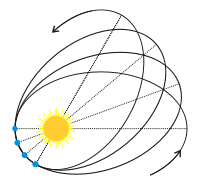
\includegraphics{figure/precessione_perielio}
  % figura presa da
  % http://commons.wikimedia.org/wiki/File:Perihelion_precession.svg
  \caption{Precessione del perielio di un pianeta}
  \label{fig:precessione-perielio}
\end{figure}
La prima legge di Keplero afferma che l'orbita descritta dai pianeti è
un'ellisse.  Questo risultato è rigorosamente vero nel caso in cui il pianeta
interagisce solo con la stella intorno a cui orbita.  La presenza di altri
eventuali pianeti perturba il sistema facendo in modo che l'orbita non sia
chiusa ma piuttosto una rosetta, si ha quindi una precessione del perielio, come
rappresentato nella figura~\ref{fig:precessione-perielio}.  Per esempio, dalle
osservazioni astronomiche si è scoperto che il perielio di Mercurio si sposta di
circa \ang{;;575} ogni cento anni.  Utilizzando la meccanica newtoniana e
tenendo conto della presenza di tutti i pianeti conosciuti si prevede una
precessione del perielio di Mercurio pari a circa \ang{;;532}.  Per spiegare
questa incongruenza sono state proposte diverse ipotesi, fra cui la presenza di
un corpo perturbante come un nuovo pianeta (Vulcano), più interno di Mercurio, o
un satellite di Mercurio.  Tuttavia questi corpi non sono mai stati trovati e
faremo vedere che la relatività generale è in grado di risolvere questo
problema.

% TODO: capire per bene i passaggi dell'Adler
Per determinare l'orbita di un pianeta abbiamo bisogno di quattro equazioni per
le quattro coordinate spazio-temporali sferiche $t$, $r$, $\theta$ e $\phi$.
Una prima equazione differenziale per la coordinata $r$ si ottiene dividendo
l'intervallo di tempo proprio di Schwarzschild~\eqref{eq:metrica-schwarzschild}
per $\dd\tau^{2}$
\begin{equation}
  \label{eq:mercurio-r}
  \bigg(\toder{\tau}{\tau}\bigg)^{2} = 1 = \bigg(1 -
  \frac{r_{\textup{S}}}{r}\bigg)\dot{t}^{2} - \bigg(1 -
  \frac{r_{\textup{S}}}{r}\bigg)^{-1}\dot{r}^{2} - r^{2}(\dot{\theta}^{2} +
  \sin^{2}\theta \dot{\phi}^{2}).
\end{equation}
Il punto sopra le variabili indica la derivazione rispetto al tempo proprio
$\tau$.  Per determinare le altre equazioni dobbiamo risolvere il problema
variazionale
\begin{equation}
  \delta \int \dd \tau = 0
\end{equation}
in cui $\dd\tau$ è la metrica di Schwarzschild.  Questo problema può essere
risolto più facilmente considerando la seguente formulazione equivalente
\begin{equation}
  \begin{split}
    \delta\int \dd\tau &= \delta \int \bigg(\toder{\tau}{\tau}\bigg)^{2} \dd
    \tau \\
    &= \delta \int \bigg(\bigg(1 - \frac{r_{\textup{S}}}{r}\bigg)\dot{t}^{2} -
    \bigg(1 - \frac{r_{\textup{S}}}{r}\bigg)^{-1}\dot{r}^{2} -
    r^{2}(\dot{\theta}^{2} + \sin^{2}\theta \dot{\phi}^{2}) \bigg) \dd \tau = 0.
  \end{split}
\end{equation}
Da qui, considerando la funzione integranda come una lagrangiana, si ottengono
tre equazioni di Eulero-Lagrange per le coordinate, rispettivamente, $\theta$,
$\phi$ e $t$
\begin{subequations}
  \begin{gather}
    \toder{}{\tau}(r^{2}\dot{\theta}) = r^{2}\sin\theta\cos\theta
    \dot{\phi}^{2}, \label{eq:mercurio-mu} \\
    \toder{}{\tau}(r^{2} \sin^{2}\theta \dot{\phi}) = 0, \label{eq:mercurio-phi}
    \\
    \toder{}{\tau}\bigg(\bigg(1 - \frac{r_{\textup{S}}}{r}\bigg) \dot{t} \bigg)
    = 0. \label{eq:mercurio-t}
  \end{gather}
\end{subequations}
Non abbiamo scritto l'equazione di Eulero-Lagrange per la coordinata $r$ poiché
utilizzeremo la~\eqref{eq:mercurio-r}.

Notiamo che associando all'equazione differenziale~\eqref{eq:mercurio-mu} le
condizioni iniziali $\theta = \pi/2$ e $\dot{\theta} = 0$, la funzione costante
$\theta(\tau) = \pi/2$ costituisce l'unica soluzione di questo problema di
Cauchy.  Ciò significa che con un'opportuna scelta delle coordinate il moto del
pianeta si svolge in un piano, così come succede anche in meccanica classica.
Sostituendo $\theta = \pi/2$ nella~\eqref{eq:mercurio-phi} abbiamo
\begin{equation}
  \label{eq:mercurio-phi2}
  \toder{}{\tau}(r^{2}\dot{\phi}) = 0 \implies r^{2}\dot{\phi} = h =
  \text{costante}
\end{equation}
cioè il pianeta si muove con velocità areolare costante, come nel problema di
Keplero classico.  Invece dalla~\eqref{eq:mercurio-t} otteniamo
\begin{equation}
  \label{eq:mercurio-t2}
  \bigg(1 - \frac{r_{\textup{S}}}{r}\bigg)\dot{t} = l = \text{costante}.
\end{equation}
Sostituendo tutti questi risultati nella~\eqref{eq:mercurio-r} troviamo
\begin{equation}
  \label{eq:mercurio-r2}
  1 = \bigg(1 - \frac{r_{\textup{S}}}{r}\bigg)^{-1}l^{2} - \bigg(1 -
  \frac{r_{\textup{S}}}{r}\bigg)^{-1}\dot{r}^{2} - \frac{h^{2}}{r^{2}}.
\end{equation}

Per determinare l'equazione dell'orbita conviene pensare la coordinata $r$ come
funzione di $\phi$, quindi indicando con l'apice la derivazione rispetto a
$\phi$ abbiamo
\begin{equation}
  \dot{r} = \toder{r}{\tau} = \toder{r}{\phi} \toder{\phi}{\tau} = r' \dot{\phi}
  = r' \frac{h}{r^{2}}
\end{equation}
e ponendo $u = 1/r$, con
\begin{equation}
  \dot{r} = \frac{h}{r^{2}}r' = \frac{h}{r^{2}}\toder{r}{\phi} =
  hu^{2}\toder{}{\phi} \frac{1}{u} = -hu^{2}\frac{u'}{u^{2}} = -hu',
\end{equation}
la~\eqref{eq:mercurio-r2} diventa
\begin{equation}
  1 - r_{\textup{S}}u = l^{2} - h^{2}u'^{2} - h^{2}u^{2}(1 - r_{\textup{S}}u),
\end{equation}
da cui, riarrangiando,
\begin{equation}
  \label{eq:mercurio-u'}
  u'^{2} = \frac{l^{2} - 1}{h^{2}} + \frac{r_{\textup{S}}}{h^{2}}u - u^{2} +
  r_{\textup{S}}u^{3} \equiv f(u).
\end{equation}
Questa equazione può essere integrata nel seguente modo
\begin{equation}
  \toder{u}{\phi} = \sqrt{f(u)} \implies \dd\phi = f^{-1/2}(u) \dd u \implies
  \phi = \phi_{0} + \int_{u_{0}}^{u} f^{-1/2}(\tilde{u}) \dd \tilde{u}.
\end{equation}
Sebbene questa sia una soluzione esatta, non è utile a livello pratico perché
fornisce solo un'espressione implicita di $u$, e quindi $r$, rispetto a $\phi$.
Nella risoluzione del problema di Keplero classico si giunge all'equazione di
Binet che è un'equazione differenziale del secondo ordine in $u$.  Per risolvere
il problema nella relatività generale, a questo punto, l'idea è quella di
ottenere un'equazione differenziale del secondo ordine in $u$ da confrontare con
l'equazione di Binet.  Derivando rispetto a $\phi$ la~\eqref{eq:mercurio-u'}
abbiamo
\begin{equation}
  \label{eq:mercurio1}
  2u'u'' = \frac{r_{\textup{S}}}{h^{2}}u' - 2uu' + 3r_{\textup{S}}u^{2}u'
  \implies u'\bigg(2u'' - \frac{r_{\textup{S}}}{h^{2}} + 2u -
  3r_{\textup{S}}u^{2}\bigg) = 0.
\end{equation}
Una soluzione di questa equazione è $u' = 0$, cioè
$u(\phi) = 1/r(\phi) = \text{costante}$.  Tuttavia questa situazione non ci
interessa poiché descrive un moto circolare, essendo la distanza dal centro del
campo costante, quindi non c'è un perielio e non è possibile osservare la sua
precessione.  L'altra possibile soluzione è
\begin{equation}
  \label{eq:binet-relativ}
  2u'' - \frac{r_{\textup{S}}}{h^{2}} + 2u - 3r_{\textup{S}}u^{2} = 0 \implies
  u'' + u = \frac{r_{\textup{S}}}{2h^{2}} + \frac{3}{2}r_{\textup{S}}u^{2} =
  \frac{GM}{r^{4}(\ltoder{\phi}{\tau})^{2}} + \frac{3}{2}r_{\textup{S}}u^{2},
\end{equation}
in cui $M$ è la massa del corpo che genera il campo gravitazionale.  Nel
problema di Keplero classico, l'\index{equazione!di Binet}equazione di Binet è
\begin{equation}
  \label{eq:binet}
  u'' + u = \frac{GM}{r^{4}(\ltoder{\phi}{t})^{2}}.
\end{equation}
Osserviamo che per piccole velocità
$\ltoder{\phi}{\tau} \approx \ltoder{\phi}{t}$.  Inoltre per i pianeti del
sistema solare risulta
\begin{equation}
  \frac{3r_{\textup{S}}u^{2}/2}{r_{\textup{S}}/(2h^{2})} = 3u^{2}h^{2} \ll 1,
\end{equation}
infatti
\begin{equation}
  3u^{2}h^{2} = \frac{3}{r^{2}}r^{4} \bigg(\toder{\phi}{\tau}\bigg)^{2} = 3r^{2}
  \bigg(\toder{\phi}{\tau}\bigg)^{2} \approx 3 v_{\textup{t}}^{2},
\end{equation}
in cui $v_{\textup{t}} = r\ltoder{\phi}{t}$ è la velocità tangenziale del corpo,
espressa in unità di $c$ poiché abbiamo posto $c = 1$.  Per Mercurio, il pianeta
più interno del sistema solare e quindi con la maggior velocità tangenziale,
$3 v_{\textup{t}}^{2} = \num{7.7e-8}$, quindi possiamo considerare il termine
$3r_{\textup{S}}u^{2}/2$ nella~\eqref{eq:binet-relativ} come una debole
perturbazione.  In dettaglio, vogliamo risolvere l'equazione
\begin{equation}
  u'' + u = A + \frac{\epsilon u^{2}}{A},
\end{equation}
con $A = r_{\textup{S}}/(2h^{2})$ e $\epsilon = 3Ar_{\textup{S}}/2  \ll 1$.
Cerchiamo soluzioni del tipo
\begin{equation}
  u(\phi) = u_{0}(\phi) + \epsilon v(\phi),
\end{equation}
con $u_{0}(\phi)$ soluzione dell'equazione di Binet classica
\begin{equation}
  \label{eq:binet-2}
  u_{0}'' + u_{0} = A
\end{equation}
cioè
\begin{equation}
  u_{0} = A + B\cos(\phi + \phi_{0}),
\end{equation}
con $B$ e $\phi_{0}$ costanti reali di integrazione.  Ruotando opportunamente il
sistema di riferimento si può fare in modo che $\phi_{0} = 0$ cosicché $u_{0}$
diventa
\begin{equation}
  \label{eq:sol-binet}
  u_{0}(\phi) = A + B\cos\phi.
\end{equation}
Dunque l'equazione da risolvere è
\begin{equation}
  (u_{0}'' + \epsilon v'') + (u_{0} + \epsilon v) = A + \epsilon \frac{(u_{0} +
    \epsilon v)^{2}}{A} = A + \epsilon \frac{u_{0}^{2}}{A} +
  \mathcal{O}(\epsilon^{2}).
\end{equation}
Tenendo conto della~\eqref{eq:binet-2} l'equazione per $v(\phi)$ al primo ordine
in $\epsilon$ è
\begin{equation}
  \begin{split}
    v'' + v &= \frac{u_{0}^{2}}{A} = A + 2B\cos\phi +
    \frac{B^{2}}{A}\cos^{2}\phi \\
    &= \bigg(A + \frac{B^{2}}{2A}\bigg) + 2B\cos\phi +
    \frac{B^{2}}{2A}\cos(2\phi),
\end{split}
\end{equation}
in cui abbiamo ricordato l'identità trigonometrica
$\cos^{2}\phi = (1 + \cos(2\phi))/2$.  Dunque questa è l'equazione differenziale
del secondo ordine relativa al termine che perturba l'orbita dei pianeti.
Questa equazione è lineare, quindi la soluzione può essere espressa come somma
delle soluzioni delle tre equazioni seguenti
\begin{subequations}
  \begin{align}
    v_{a}'' + v_{a} &= A + \frac{B^{2}}{2A} \implies v_{a}(\phi) = A +
    \frac{B^{2}}{2A}, \\
    v_{b}'' + v_{b} &= 2B\cos\phi \implies v_{b}(\phi) = B\phi \sin\phi, \\
    v_{c}'' + v_{c} &= \frac{B^{2}}{2A}\cos(2\phi) \implies v_{c}(\phi) =
    -\frac{B^{2}}{6A}\cos(2\phi),
  \end{align}
\end{subequations}
dunque
\begin{equation}
  v(\phi) = v_{a}(\phi) + v_{b}(\phi) + v_{c}(\phi) = A + \frac{B^{2}}{2A} +
  B\phi\sin\phi - \frac{B^{2}}{6A}\cos(2\phi)
\end{equation}
e in questo modo $u(\phi)$ è data da
\begin{equation}
  \begin{split}
    u(\phi) &= u_{0}(\phi) + \epsilon v(\phi) \\
    &= A + B\cos\phi + \epsilon A + \frac{\epsilon B^{2}}{2A} + \epsilon
    B\phi\sin\phi - \frac{\epsilon B^{2}}{6A}\cos(2\phi).
  \end{split}
\end{equation}
Al primo ordine in $\epsilon$ abbiamo
\begin{equation}
  \cos(\phi - \epsilon\phi) = \cos\phi \cos(\epsilon\phi) + \sin\phi
  \sin(\epsilon\phi) \approx \cos\phi + \epsilon\phi\sin\phi,
\end{equation}
allora
\begin{equation}
  \frac{1}{r(\phi)} = u(\phi) \approx A + B\cos(\phi - \epsilon\phi) +
  \epsilon\bigg(A + \frac{B^{2}}{2A} - \frac{B^{2}}{6A}\cos(2\phi)\bigg).
\end{equation}
L'ultimo termine, fra parentesi, induce una piccola variazione nella distanza
radiale del pianeta, ma non può essere responsabile della precessione del
perielio poiché il termine $\cos(2\phi)$ ha periodo sottomultiplo intero di
$2\pi$ (quindi dopo un'intera rivoluzione di $\var \phi = 2\pi$ assume di nuovo
lo stesso valore).  Il resto della funzione $u(\phi)$ si differenzia dalla
soluzione~\eqref{eq:sol-binet} dell'equazione di Binet per la presenza di
$-\epsilon\phi$ nell'argomento del coseno.  Il perielio si ha quando $r(\phi)$ è
minimo, vale a dire quando $u(\phi)$ è massimo e ciò si verifica quando il
coseno del secondo termine vale $1$, cioè quando
\begin{equation}
  \phi_{n}(1 - \epsilon) = 2\pi n \implies \phi_{n} = \frac{2\pi n}{1 -
    \epsilon} \approx 2\pi n(1 + \epsilon)
\end{equation}
con $n$ numero di rivoluzioni compiute dal pianeta intorno al Sole a partire da
un istante iniziale fissato.  Il perielio successivo si ha dopo una variazione
della coordinata $\phi$ di
\begin{equation}
  \var\phi = \phi_{n+1} - \phi_{n} = 2\pi(1 + \epsilon)
\end{equation}
invece di $2\pi$ come succede per un'orbita chiusa.  La relatività generale
prevede allora una precessione del perielio dei pianeti nel loro moto intorno al
Sole, indipendentemente dalla presenza perturbatrice di altri corpi.  Stimiamo
il valore $\delta\phi$ di questa precessione per verificare se è in accordo con
i dati sperimentali.  Per i pianeti del sistema solare
$r_{\textup{S}} = 2GM_{\odot}$ è il raggio di Schwarzschild del Sole, allora
\begin{equation}
  \delta\phi = 2\pi\epsilon = 2\pi \frac{3}{4}\frac{r_{\textup{S}}^{2}}{h^{2}} =
  6\pi \frac{G^{2}M_{\odot}^{2}}{h^{2}}.
\end{equation}
In particolare per il pianeta Mercurio si ha
\begin{equation}
  \delta\phi = \ang{;;0.1036}
\end{equation}
e la precessione dopo cento anni, ricordando che il suo periodo orbitale è di
$87.8$ giorni, è data da
\begin{equation}
  \delta_{100}\phi = \frac{\delta\phi \cdot 100 \cdot 365.25}{87.8} =
  \ang{;;43}.
\end{equation}
All'inizio della sezione abbiamo ricordato che la precessione secolare di
Mercurio è di circa \ang{;;575}, possiamo ora concludere che di questi, circa
\ang{;;43} sono dovuti a effetti di relatività generale e circa \ang{;;532} alla
perturbazione indotta dalla presenza degli altri pianeti.  Mercurio è il pianeta
del sistema solare per il quale la precessione relativistica del perielio è più
evidente in quanto è il più interno e quindi il più influenzato dal campo
gravitazionale del Sole.

\subsection{Deflessione della luce}
\label{sec:deflessione-luce}

Secondo la teoria newtoniana, solo i corpi dotati di massa sono soggetti
all'attrazione gravitazionale.  In questo paragrafo vedremo che un fotone (così
come qualsiasi corpo privo di massa) risente della presenza di un campo
gravitazionale, come quello generato dal Sole, deviando la propria traiettoria.
Questo fenomeno è comprensibile ricordando che tutti i corpi si muovono lungo
geodetiche in uno spazio-tempo curvo.

% TODO: non ho mai classificato gli intervalli nei tipi `luce', `spazio' o
% `tempo', quindi o lo faccio da qualche parte o riformulo la frase seguente.
% Dovrei anche spiegare cos'è la linea d'universo.
In relatività speciale, per due eventi separati da un intervallo di tipo luce la
distanza vale $\dd\tau^{2} = 0$ e assumiamo che lo stesso valga anche in
relatività generale.  Assumiamo inoltre che l'equazione della
geodetica~\eqref{eq:geodetica} sia valida anche per le particelle prive di massa
come i fotoni.  Tuttavia dobbiamo fare attenzione al fatto che, proprio in virtù
del fatto che $\dd\tau^{2} = 0$, non possiamo parametrizzare la linea d'universo
di un fotone, o di una qualsiasi particella con massa nulla, usando il tempo
proprio $\tau$.  Piuttosto dobbiamo utilizzare un differente parametro $q$ tale
che l'equazione della geodetica
\begin{equation}
  \toder[2]{x^{\mu}}{q} + \tensor{\Gamma}{^{\mu}_{\lambda\nu}}
  \toder{x^{\lambda}}{q} \toder{x^{\nu}}{q} = 0
\end{equation}
abbia senso.  A partire da questa equazione si possono ricavare nuovamente,
sempre con l'assunzione $\theta = \pi/2$, le relazioni~\eqref{eq:mercurio-phi2}
e \eqref{eq:mercurio-t2}.  La~\eqref{eq:mercurio-r2} va modificata in questo
modo tenendo conto del fatto che $\dd\tau^{2} = 0$
\begin{equation}
  0 = \bigg(1 - \frac{r_{\textup{S}}}{r}\bigg)^{-1}l^{2} - \bigg(1 -
  \frac{r_{\textup{S}}}{r}\bigg)^{-1}\dot{r}^{2} - \frac{h^{2}}{r^{2}}.
\end{equation}
Svolgendo i calcoli in maniera analoga a quanto visto nel paragrafo precedente e
ponendo sempre $u = 1/r$ si arriva all'equazione
\begin{equation}
  u'\bigg(u'' + u - \frac{3}{2}r_{\textup{S}}u^{2}\bigg) = 0.
\end{equation}
Si possono avere due situazioni:
\begin{equation}
  \label{eq:deflessione1}
  u'' + u - \frac{3}{2}r_{\textup{S}}u^{2} = 0,
\end{equation}
oppure
\begin{equation}
  u' = 0 \implies u(\phi) = u_{0} = \text{costante},
\end{equation}
ma quest'ultima soluzione deve essere scartata per ragioni di stabilità.
Osserviamo che si poteva giungere direttamente alla~\eqref{eq:deflessione1}
partendo dalla~\eqref{eq:mercurio1} e ponendo
$\dd\tau^{2} = 0 \implies 1/h^{2} = (\ltoder{\tau}{\phi})^{2}/r^{4} = 0$.  Il
termine $3r_{\textup{S}}u^{2}/2$ è una piccola perturbazione rispetto a $u$,
infatti
\begin{equation}
  \frac{3r_{\textup{S}}u^{2}/2}{u} = \frac{3r_{\textup{S}}u}{2} =
  \frac{3r_{\textup{S}}}{2r}.
\end{equation}
Considerando il caso del Sole, $r_{\textup{S}} = \SI{3}{\kilo\metre}$ e la
distanza $r$ rispetto alla sua origine a cui un fotone può passare è maggiore o
uguale al raggio $R_{\odot} = \SI{7e5}{\kilo\metre}$, quindi
$3r_{\textup{S}}u^{2}/(2u) \ll 1$.  Allora cerchiamo una soluzione dell'equazione
\begin{equation}
  u'' + u = \epsilon u^{2},
\end{equation}
con $\epsilon = 3r_{\textup{S}}/2$, del tipo
\begin{equation}
  u(\phi) = u_{0}(\phi) + \epsilon v(\phi).
\end{equation}
Sostituendo nell'equazione da risolvere abbiamo
\begin{equation}
  \label{eq:deflessione2}
  u_{0}'' + u_{0} + \epsilon v'' + \epsilon v = \epsilon u_{0}^{2} +
  \mathcal{O}(\epsilon^{2}).
\end{equation}
I termini di ordine zero in $\epsilon$ danno
\begin{equation}
  u_{0}'' + u_{0} = 0,
\end{equation}
la cui soluzione generale è
\begin{equation}
  u_{0}(\phi) = A\cos(\phi + \phi_{0}),
\end{equation}
con $A$ e $\phi_{0}$ costanti di integrazione.  Ruotando il sistema di
coordinate è possibile annullare $\phi_{0}$ cosicché il valore approssimato
$r = 1/u_{0}$ della coordinata radiale soddisfi la relazione
\begin{equation}
  r \cos\phi = \frac{1}{A} = \text{costante}.
\end{equation}
Il prodotto $r\cos\phi$ è la coordinata cartesiana $x$, quindi questa è
l'equazione di una retta parallela all'asse $y$.  Potevamo attenderci questo
risultato: in prima approssimazione il raggio di luce non viene deviato dal
campo gravitazionale del Sole.  Inoltre la distanza $r_{0}$ di minimo
avvicinamento al corpo si ha per $\cos\phi = 1$, cioè
$r_{0} = 1/A \implies u_{0} = (\cos\phi)/r_{0}$.  Uguagliando i termini di
ordine uno in $\epsilon$ troviamo
\begin{equation}
  \label{eq:deflessione3}
  v'' + v = u_{0}^{2} = \frac{\cos^{2}\phi}{r_{0}^{2}} = \frac{1 +
    \cos(2\phi)}{2r_{0}^{2}}.
\end{equation}
Cerchiamo soluzioni del tipo
\begin{equation}
  v(\phi) = \alpha + \beta\cos(2\phi)
\end{equation}
con $\alpha$ e $\beta$ costanti di integrazione da determinare.  Sostituendo
nella~\eqref{eq:deflessione3} otteniamo
\begin{equation}
  v'' + v = \alpha - 3\beta\cos(2\phi).
\end{equation}
Confrontando con la~\eqref{eq:deflessione3} abbiamo
\begin{subequations}
  \begin{align}
    \alpha &= \frac{1}{2r_{0}^{2}}, \\
    \beta &= - \frac{1}{6r_{0}^{2}},
  \end{align}
\end{subequations}
quindi
\begin{equation}
  v(\phi) = \frac{1}{2r_{0}^{2}} - \frac{\cos(2\phi)}{6r_{0}^{2}} =
  \frac{2}{3r_{0}^{2}} - \frac{\cos^{2}\phi}{3r_{0}^{2}}.
\end{equation}
In definitiva
\begin{equation}
  \label{eq:deflessione4}
  u(\phi) = u_{0}(\phi) + \epsilon v(\phi) = \frac{\cos\phi}{r_{0}} +
  \frac{2\epsilon}{3r_{0}^{2}} - \frac{\epsilon\cos^{2}\phi}{3r_{0}^{2}}.
\end{equation}
% TODO: fare una figura altrimenti si capisce piuttosto poco e riformulare il
% testo seguente in modo da adattarsi alla figura.
La traiettoria del fotone è, dunque, una retta (data dal termine
$(\cos\phi)/r_{0}$) disturbata da una piccola perturbazione dell'ordine di
$\epsilon$.  L'effetto di questa perturbazione è il seguente: il fotone si
avvicina al Sole in linea retta, quando l'influenza del campo gravitazionale
della stella non è più trascurabile il fotone viene leggermente deflesso, quindi
si allontana nuovamente in linea retta.  Calcoliamo la deflessione del fotone.
Le direzioni asintotiche seguite dal fotone si ottengono calcolando il limite
$r \to \infty$ o, il che è equivalente, $u \to 0$ nella~\eqref{eq:deflessione4}
\begin{equation}
  0 = \frac{\cos\phi}{r_{0}} + \frac{2\epsilon}{3r_{0}^{2}} -
  \frac{\epsilon\cos^{2}\phi}{3r_{0}^{2}} \implies \cos^{2}\phi -
  \frac{3r_{0}}{\epsilon}\cos\phi - 2 = 0.
\end{equation}
Le soluzioni sono
\begin{equation}
  \cos\phi = \frac{3r_{0}}{2\epsilon}\bigg(1 \pm \sqrt{1 +
    \frac{8\epsilon^{2}}{9r_{0}^{2}}}\bigg),
\end{equation}
ma l'unica accettabile è quella con il segno $-$, poiché quella con il segno $+$
rende il coseno maggiore di $1$.  Sviluppando la soluzione accettabile al primo
ordine in $\epsilon$ abbiamo
\begin{equation}
  \cos\phi = \frac{3r_{0}}{2\epsilon}\bigg(1 - \sqrt{1 +
    \frac{8\epsilon^{2}}{9r_{0}^{2}}}\bigg) \approx \frac{3r_{0}}{2\epsilon}\bigg(1 - 1 -
  \frac{4\epsilon^{2}}{9r_{0}^{2}}\bigg) = -\frac{2\epsilon}{3r_{0}} =
  -\frac{r_{\textup{S}}}{r_{0}}.
\end{equation}
Abbiamo già osservato che per i fotoni che passano nelle vicinanze del Sole
risulta $r_{\textup{S}}/r \ll 1$, quindi $\phi \approx \pm \pi/2$, allora
possiamo porre $\phi = \pi/2 + \delta$, con $\delta \ll 1$, da cui
\begin{equation}
  -\frac{r_{\textup{S}}}{r_{0}} = \cos\phi = \cos(\pi/2 + \delta) = -\sin\delta.
\end{equation}
Dal momento che $\delta$ è molto piccolo possiamo approssimare il seno
dell'angolo con l'angolo stesso e quindi
\begin{equation}
  \delta = \frac{r_{\textup{S}}}{r_{0}}.
\end{equation}
La deflessione $\var$ è il doppio di questo angolo, dunque, ripristinando il
valore della velocità della luce,
\begin{equation}
  \var = 2\delta = \frac{2r_{\textup{S}}}{r_{0}} = \frac{4GM}{c^{2}r_{0}}.
\end{equation}

Per quanto riguarda la deviazione dei raggi di luce da parte del campo
gravitazionale del Sole, supponendo che la distanza di minimo avvicinamento sia
proprio pari al raggio solare $R_{\odot}$, l'angolo di deflessione vale
\begin{equation}
  \var_{\odot} = \frac{4GM_{\odot}}{c^{2}R_{\odot}} = \ang{;;1.75}.
\end{equation}
Questa previsione teorica è stata confermata in numerosi esperimenti via via più
accurati, il primo dei quali fu realizzato da Eddington durante l'eclissi totale
di Sole del 1919.

\subsection{Ritardo dei segnali radar}
\label{sec:ritardo-radar}

L'ultimo fenomeno di cui ci interessiamo è il ritardo nel tempo di volo dei
segnali radar rispetto a quanto previsto dalla relatività speciale in uno
spazio-tempo piatto.  Ciò è dovuto al fatto che i fotoni non si muovono lungo
linee rette ma lungo le geodetiche, che hanno lunghezza maggiore rispetto alle
linee rette in uno spazio-tempo piatto.  Questo fenomeno può essere osservato
inviando un segnale radar a un pianeta in congiunzione superiore e misurando il
tempo necessario affinché il segnale vada verso il pianeta e torni sulla Terra.
Tuttavia l'esecuzione di esperimenti su questo fenomeno presentano delle
difficoltà di tipo pratico, delle quali non ci occuperemo.

% TODO: mettere anche qui una figura e rielaborare il testo altrimenti non si
% capisce niente.  Dopo aver fatto la figura, parlare in generale di distanza di
% minimo avvicinamento piuttosto che di raggio solare.
Senza entrare nei dettagli dei conti forniamo i risultati delle previsioni
teoriche della relatività
generale.\footnote{Questo problema è trattato da
  \textcite[1103-1109]{misner:gravitation},
  \textcite[201-207]{weinberg:gravitation}.}
In un spazio-tempo piatto, il tempo $\tau(r,R_{\odot})$ necessario per un fotone
per giungere tangente sulla superficie del Sole da un punto a distanza $r$ dal
centro della stella è dato semplicemente dal rapporto fra la distanza euclidea
fra questi due punti e la velocità dei fotoni nel vuoto
\begin{equation}
  \tau(r, R_{\odot}) = \frac{\sqrt{r^{2} - R_{\odot}^{2}}}{c}.
\end{equation}
La correzione relativistica per $\tau(r, R_{\odot})$, che tiene conto della
curvatura dello spazio tempo prodotta dal campo gravitazionale del Sole, è
\begin{equation}
  \begin{split}
    t(r,R_{\odot}) &\approx \tau(r,R_{\odot}) + \var t(r,R_{\odot}) \\
    &= \frac{\sqrt{r^{2} - R_{\odot}^{2}}}{c} + \frac{2GM_{\odot}}{c^{3}} \ln
    \frac{r + \sqrt{r^{2} - R_{\odot}^{2}}}{R_{\odot}} +
    \frac{GM_{\odot}}{c^{3}} \sqrt{\frac{r - R_{\odot}}{r + R_{\odot}}}.
  \end{split}
\end{equation}
Il tempo $t_{\textup{tot}}$ totale di volo del fotone per andare dalla Terra, a
distanza $r_{1}$ dal Sole, a un pianeta a distanza $r_{2}$ in congiunzione
superiore è
\begin{equation}
  \begin{split}
    t_{\textup{tot}} &= 2(t(r_{1},R_{\odot}) + t(r_{2},R_{\odot})) \\
    &= 2(\tau(r_{1},R_{\odot}) + \var t(r_{1},R_{\odot}) +
    \tau(r_{2},R_{\odot}) + \var t(r_{2},R_{\odot})).
  \end{split}
\end{equation}
Considerando il sistema Terra-Mercurio, il ritardo
$\var t = 2(\var t(r_{1},R_{\odot}) + \var t(r_{2},R_{\odot}))$ rispetto alla
previsione $2(\tau(r_{1},R_{\odot}) + \tau(r_{2},R_{\odot}))$ in uno
spazio-tempo piatto vale \SI{240}{\micro\second}, che corrisponde a una distanza
di \SI{72}{\kilo\metre}, su un tempo di volo totale $t_{\textup{tot}}$ di
\SI{20}{\minute}.

%%% Local Variables:
%%% mode: latex
%%% TeX-master: "../gravitazione"
%%% fill-column: 80
%%% End:

\chapter{Onde gravitazionali}
\label{cha:onde-grav}

Nel paragrafo~\ref{sec:campo-statico-sferico} abbiamo risolto le equazioni di
Einstein nel vuoto in un campo a simmetria sferica.  In questo capitolo ci
occuperemo della risoluzione delle equazioni di Einstein nel vuoto e
nell'approssimazione di campo debole, quindi ci serviremo di alcuni risultati
trovati nei paragrafi~\ref{sec:limite-newtoniano} e
\ref{sec:limite-newtoniano-einstein}.  Troveremo che il campo gravitazionale può
emettere radiazione, analogamente a quanto succede per il campo
elettromagnetico, come abbiamo visto nel
paragrafo~\ref{sec:onde-elettromagnetiche}.  Sebbene questo risultato sarà
ottenuto nell'approssimazione di campo debole, è un fatto del tutto generale, ma
la trattazione non approssimata presenta notevoli difficoltà matematiche legate
alla non linearità delle equazioni di Einstein.

\section{Approssimazione di campo debole}
\label{sec:approx-campo-debole-onde}

Ricordiamo che nell'approssimazione di campo debole il tensore metrico
covariante è dato da
\begin{equation}
  g_{\mu\nu} = \eta_{\mu\nu} + h_{\mu\nu},
\end{equation}
con $\abs{h_{\mu\nu}} \ll 1$, mentre il tensore metrico controvariante è
\begin{equation}
  g^{\mu\nu} = \eta^{\mu\nu} - h^{\mu\nu},
\end{equation}
con $h^{\mu\nu} = \eta^{\mu\lambda}\eta^{\mu\sigma} h^{\lambda\sigma}$.
L'innalzamento e l'abbassamento degli indici di $h_{\mu\nu}$ si esegue con il
tensore metrico non perturbato $\eta_{\mu\nu}$.
Dalla~\eqref{eq:christoffel-approx} abbiamo che la connessione affine
approssimata al primo ordine in $h_{\mu\nu}$ è
\begin{equation}
  \tensor{\Gamma}{^{\lambda}_{\mu\nu}} \approx \frac{1}{2}\eta^{\sigma\lambda}
  (\partial_{\mu}h_{\nu\sigma} + \partial_{\nu}h_{\mu\sigma}
  - \partial_{\sigma}h_{\mu\nu})
\end{equation}
e quindi il tensore di Ricci, trascurando i termini superiori al primo ordine in
$h_{\mu\nu}$, è dato da
\begin{equation}
  \begin{split}
    R_{\mu\nu} &= \partial_{\nu}\tensor{\Gamma}{^{\lambda}_{\mu\lambda}}
    - \partial_{\lambda} \tensor{\Gamma}{^{\lambda}_{\mu\nu}} +
    \overbrace{\tensor{\Gamma}{^{\eta}_{\mu\lambda}}
      \tensor{\Gamma}{^{\lambda}_{\eta\nu}} -
      \tensor{\Gamma}{^{\eta}_{\mu\nu}}
      \tensor{\Gamma}{^{\lambda}_{\eta\lambda}}}^{\mathcal{O}(h^{2})}
    \approx \partial_{\nu}\tensor{\Gamma}{^{\lambda}_{\mu\lambda}}
    - \partial_{\lambda} \tensor{\Gamma}{^{\lambda}_{\mu\nu}} \\
    &= \frac{1}{2}\partial_{\nu} (\eta^{\lambda\sigma}(\partial_{\mu}
    h_{\sigma\lambda} + \partial_{\lambda}h_{\mu\sigma}
    - \partial_{\sigma}h_{\mu\lambda})) -
    \frac{1}{2}\partial_{\lambda}(\eta^{\lambda\sigma}(\partial_{\mu}h_{\sigma\nu}
    + \partial_{\nu}h_{\mu\sigma} - \partial_{\sigma}h_{\mu\nu})) \\
    &= \frac{1}{2} \eta^{\lambda\sigma}(\partial_{\mu}\partial_{\nu}
    h_{\sigma\lambda} + \partial_{\lambda}\partial_{\nu} h_{\mu\sigma}
    - \partial_{\sigma}\partial_{\nu} h_{\mu\lambda}
    - \partial_{\mu}\partial_{\lambda} h_{\sigma\nu}
    - \partial_{\nu}\partial_{\lambda} h_{\mu\sigma}
    + \partial_{\sigma}\partial_{\lambda} h_{\mu\nu}) \\
    &= \frac{1}{2}(\partial_{\mu}\partial_{\nu}
    \tensor{h}{^{\lambda}_{\lambda}} - \partial^{\lambda}\partial_{\nu}
    h_{\mu\lambda} - \partial^{\lambda}\partial_{\mu} h_{\nu\lambda}
    + \partial_{\lambda}\partial^{\lambda} h_{\mu\nu}) \\
    &= \frac{1}{2} (\dalamb h_{\mu\nu} + \partial_{\mu}\partial_{\nu} h
    - \partial^{\lambda}\partial_{\nu} h_{\mu\lambda}
    - \partial_{\mu}\partial^{\lambda} h_{\nu\lambda}),
  \end{split}
\end{equation}
in cui $h = \tensor{h}{^{\lambda}_{\lambda}} = \eta^{\mu\lambda} h_{\mu\lambda}$
è la contrazione della perturbazione.  Nel vuoto allora abbiamo
\begin{equation}
  R_{\mu\nu} = \frac{1}{2} (\dalamb h_{\mu\nu} + \partial_{\mu}\partial_{\nu} h
  - \partial^{\lambda}\partial_{\nu} h_{\mu\lambda}
  - \partial_{\mu}\partial^{\lambda} h_{\nu\lambda}) = 0.
\end{equation}

A questo punto vogliamo manipolare l'espressione ottenuta per il tensore di
Ricci in modo che le equazioni di Einstein nel vuoto si linearizzino, diventando
analoghe alle equazioni di Maxwell nel vuoto $\dalamb A_{\beta} = 0$.  Come nel
caso elettromagnetico, è possibile fare ciò scegliendo una gauge opportuna.  In
questo caso conviene scegliere la \index{gauge!armonica}\emph{gauge armonica}
\begin{equation}
  \label{eq:gauge-armonica}
  \partial_{\mu} \tensor{h}{^{\mu}_{\nu}} =
  \frac{1}{2}\partial_{\nu}\tensor{h}{^{\mu}_{\mu}}.
\end{equation}
Infatti usando questa gauge gli ultimi tre termini del tensore di Ricci si
annullano
\begin{equation}
  \begin{split}
    \partial_{\mu}\partial_{\nu} h - \partial^{\lambda}\partial_{\nu}
    h_{\mu\lambda} - \partial_{\mu}\partial^{\lambda} h_{\nu\lambda}
    &= \partial_{\mu}(2 \partial_{\lambda}\tensor{h}{^{\lambda}_{\nu}})
    - \partial_{\nu}(\partial_{\lambda}\tensor{h}{^{\lambda}_{\mu}})
    - \partial_{\lambda}\partial_{\mu} \tensor{h}{^{\lambda}_{\nu}} \\
    &= \partial_{\mu}\partial_{\lambda} \tensor{h}{^{\lambda}_{\nu}}
    - \partial_{\nu}(\partial_{\lambda} \tensor{h}{^{\lambda}_{\mu}}) \\
    &= \partial_{\mu}\bigg(\frac{1}{2}\partial_{\nu}
    \tensor{h}{^{\lambda}_{\lambda}}\bigg)
    - \partial_{\nu}\bigg(\frac{1}{2}\partial_{\mu}
    \tensor{h}{^{\lambda}_{\lambda}}\bigg) = 0
  \end{split}
\end{equation}
e quindi $R_{\mu\nu} = \dalamb h_{\mu\nu}/2$.  Le equazioni di Einstein nel
vuoto si possono, in questo modo, scrivere nella seguente forma lineare
\begin{equation}
  \label{eq:einstein-lineare}
  \dalamb h_{\mu\nu} = 0.
\end{equation}
Osserviamo che la condizione di gauge armonica~\eqref{eq:gauge-armonica} si può
anche porre nella forma
$\Gamma^{\lambda} = \eta^{\mu\nu} = \tensor{\Gamma}{^{\lambda}_{\mu\nu}} = 0$ in
quanto
\begin{equation}
  \begin{split}
    0 &=\eta^{\mu\nu} \tensor{\Gamma}{^{\lambda}_{\mu\nu}} = \frac{1}{2}
    \eta^{\lambda\sigma} (\partial^{\mu}h_{\mu\sigma} + \partial^{\mu}
    h_{\mu\sigma} - \partial_{\sigma}\tensor{h}{^{\mu}_{\mu}}) \\
    &= \frac{1}{2} (\partial^{\mu} \tensor{h}{_{\mu}^{\lambda}} + \partial^{\mu}
    \tensor{h}{_{\mu}^{\lambda}} - \partial^{\lambda} \tensor{h}{^{\mu}_{\mu}}),
  \end{split}
\end{equation}
da cui
\begin{equation}
  \partial^{\lambda} \tensor{h}{^{\mu}_{\mu}} = 2 \partial^{\mu}
  \tensor{h}{_{\mu}^{\lambda}}
\end{equation}
che equivale alla~\eqref{eq:gauge-armonica}.

Si può sempre scegliere un sistema di riferimento in cui sia valida la
condizione armonica.  Sia $x^{\mu}$ un sistema di coordinate in cui questa
condizione non è valida, allora possiamo effettuare la trasformazione
infinitesima $x^{\mu} \to x'^{\mu} = x^{\mu} + \epsilon^{\mu}(x)$, con
$\abs{\epsilon^{\mu}(x)} \ll 1$, richiedendo che la metrica si possa ancora
sviluppare come $g'_{\mu\nu} = \eta_{\mu\nu} + h'_{\mu\nu}$, in modo da poter
ancora ottenere la forma linearizzata~\eqref{eq:einstein-lineare} delle
equazioni di Einstein.  Possiamo determinare un'espressione esplicita per
$h'_{\mu\nu}$ imponendo che il tensore metrico controvariante nel nuovo sistema
$g'^{\mu\nu} = \eta^{\mu\nu} - h'^{\mu\nu}$ si trasformi come un tensore
controvariante di rango $2$.  Trascurando termini del secondo ordine in
$\epsilon$ o dell'ordine di $h\epsilon$ abbiamo
\begin{equation}
  \begin{split}
    g'^{\mu\nu} &=
    g^{\lambda\rho} \parder{x'^{\mu}}{x^{\lambda}} \parder{x'^{\nu}}{x^{\rho}} =
    (\eta^{\lambda\rho} + h^{\lambda\rho}) (\tensor{\delta}{^{\mu}_{\lambda}}
    + \partial_{\lambda}\epsilon^{\mu}) (\tensor{\delta}{^{\nu}_{\rho}}
    + \partial_{\rho} \epsilon^{\nu}) \\
    &= (\eta^{\mu\rho} - h^{\mu\rho} +
    \eta^{\lambda\rho}\partial_{\lambda}\epsilon^{\mu} -
    \underbrace{h^{\lambda\rho} \partial_{\lambda}
      \epsilon^{\mu}}_{\mathcal{O}(h\epsilon)})
    (\tensor{\delta}{^{\nu}_{\rho}} + \partial_{\rho} \epsilon^{\nu}) \\
    &\approx \eta^{\mu\nu} - h^{\mu\nu} + \eta^{\lambda\nu}\partial_{\lambda}
    \epsilon^{\mu} + \eta^{\mu\rho}\partial_{\rho} \epsilon^{\nu} -
    \underbrace{h^{\mu\rho}\partial_{\rho}\epsilon^{\nu}}_{\mathcal{O}(h\epsilon)}
    + \underbrace{\partial^{\rho} \epsilon^{\mu} \partial_{\rho}
      \epsilon^{\nu}}_{\mathcal{O}(\epsilon^{2})} \\
    & \approx \eta^{\mu\nu} - h^{\mu\nu} + \partial^{\nu} \epsilon^{\mu}
    + \partial^{\mu} \epsilon^{\nu}.
  \end{split}
\end{equation}
Dunque
\begin{equation}
  h'^{\mu\nu} = h^{\mu\nu} - \partial^{\nu} \epsilon^{\mu} + \partial^{\mu}
  \epsilon^{\nu}.
\end{equation}
In questo nuovo sistema di riferimento calcoliamo ambo i membri
della~\eqref{eq:gauge-armonica}
\begin{equation}
  \begin{split}
    &\partial_{\mu} \tensor{{h'}}{^{\mu}_{\nu}} = \frac{1}{2}\partial_{\nu}
    \tensor{{h'}}{^{\mu}_{\mu}} \iff \\
    &\partial_{\mu} \tensor{h}{^{\mu}_{\nu}}
    - \partial_{\mu} \partial_{\nu} \epsilon^{\nu}
    - \partial_{\mu}\partial^{\mu} \epsilon_{\nu}
    = -\frac{1}{2} \partial_{\nu} \partial_{\mu} \epsilon^{\mu} -
    \frac{1}{2}\partial_{\nu} \partial_{\mu} \epsilon^{\mu} +
    \frac{1}{2} \partial_{\nu} \tensor{h}{^{\mu}_{\mu}} \iff \\
    &\partial_{\mu} \tensor{h}{^{\mu}_{\nu}}
    - \partial_{\mu}\partial^{\mu} \epsilon_{\nu}
    = \frac{1}{2} \partial_{\nu} \tensor{h}{^{\mu}_{\mu}}.
  \end{split}
\end{equation}
Quindi se scegliamo il generatore $\epsilon_{\nu}$ della trasformazione
infinitesima delle coordinate tale che
\begin{equation}
  \dalamb \epsilon_{\nu} = \partial_{\mu} \tensor{h}{^{\mu}_{\nu}} -
  \frac{1}{2} \partial_{\nu} \tensor{h}{^{\mu}_{\mu}}
\end{equation}
allora nel nuovo sistema di riferimento la condizione
armonica~\eqref{eq:gauge-armonica} sarà soddisfatta.  Se la condizione era già
valida nel sistema di partenza, bisognerà allora porre
$\dalamb \epsilon_{\nu} = 0$.  Questa libertà di scelta ricorda la libertà che
si ha nella gauge di Lorenz per il potenziale elettromagnetico.

Abbiamo visto che con la gauge armonica~\eqref{eq:gauge-armonica} l'equazione di
Einstein nel vuoto può essere scritta nella forma
lineare~\eqref{eq:einstein-lineare}, che è del tutto analoga alle equazioni di
Maxwell~\eqref{eq:maxwell-vuoto-lorenz} nel vuoto con la gauge di Lorenz, quindi
anche per $h_{\mu\nu}$ la soluzione generale sarà una sovrapposizione lineare di
onde piane del tipo
\begin{equation}
  h_{\mu\nu} = \Re\{e_{\mu\nu} \e^{\uimm k^{\lambda}x_{\lambda}} \}.
\end{equation}
Queste sono le \index{onda!gravitazionale}\emph{onde gravitazionali}.
Dalla~\eqref{eq:einstein-lineare} abbiamo (omettendo il simbolo $\Re$ per quanto
detto nel paragrafo~\ref{sec:onde-elettromagnetiche})
\begin{equation}
  0 = \dalamb h_{\mu\nu} = \uimm k^{\lambda} \uimm k_{\lambda} e_{\mu\nu}
  \e^{\uimm k^{\lambda}x_{\lambda}} \implies k^{\lambda}k_{\lambda} = 0,
\end{equation}
cioè le onde si muovono, come quelle elettromagnetiche, alla velocità della luce
nel vuoto.  Inoltre dalla gauge armonica~\eqref{eq:gauge-armonica} abbiamo
\begin{equation}
  \uimm k_{\lambda} \tensor{e}{^{\lambda}_{\nu}} \e^{\uimm
    k^{\lambda}x_{\lambda}} = \frac{\uimm}{2} k_{\nu}
  \tensor{e}{^{\lambda}_{\lambda}} \e^{\uimm k^{\lambda}x_{\lambda}} \iff
  k_{\lambda} \tensor{e}{^{\lambda}_{\nu}} = \frac{1}{2} k_{\nu}
  \tensor{e}{^{\lambda}_{\lambda}}.
\end{equation}
Dal momento che $h_{\mu\nu}$ è simmetrico nello scambio degli indici, lo dovrà
essere anche $e_{\mu\nu}$, chiamato \index{tensore!di polarizzazione}
\emph{tensore di polarizzazione}, il quale quindi avrà indipendenti al più dieci
delle sue sedici componenti.  Al variare di $\nu$ nell'equazione precedente ci
sono quattro ulteriori relazioni che legano le componenti del tensore di
polarizzazione, quindi il numero di componenti indipendenti non può superare
sei.

Scegliamo l'asse $z$ lungo la direzione di propagazione dell'onda, di modo
che il vettore d'onda abbia la forma
$k^{\mu} = (k^{0}, k^{1}, k^{2}, k^{3}) = (k, 0, 0, k)$.  Ponendo nell'equazione
precedente $\nu = 1$ abbiamo
\begin{equation}
  k_{\mu}\tensor{e}{^{\mu}_{1}} = \frac{1}{2} k_{1}\tensor{e}{^{\mu}_{\mu}} = 0.
\end{equation}
Esplicitiamo il primo membro
\begin{equation}
  k_{0} \tensor{e}{^{0}_{1}} + k_{3} \tensor{e}{^{3}_{1}} = 0 \implies
  \tensor{e}{^{0}_{1}} = -\tensor{e}{^{3}_{1}} \implies e_{01} = -e_{31}.
\end{equation}
Analogamente per $\nu = 2$ si trova
\begin{equation}
  k_{\mu} \tensor{e}{^{\mu}_{2}} = \frac{1}{2} k_{2} \tensor{e}{^{\mu}_{\mu}} =
  0 \implies e_{02} = -e_{32}.
\end{equation}
Per $\nu = 0$ risulta
\begin{equation}
  \begin{split}
    &k_{\mu} \tensor{e}{^{\mu}_{0}} = \frac{1}{2} k_{0}\tensor{e}{^{\mu}_{\mu}}
    = \frac{1}{2}\eta_{00}k^{0}\tensor{e}{^{\mu}_{\mu}} =
    -\frac{1}{2}k^{0}\tensor{e}{^{\mu}_{\mu}} \implies \\
    &k^{0} e_{00} + k^{3}e_{30} = -\frac{1}{2}k^{0}(\tensor{e}{^{1}_{1}} +
    \tensor{e}{^{2}_{2}} + \tensor{e}{^{3}_{3}} - e_{00})
  \end{split}
\end{equation}
e poiché $\tensor{e}{^{i}_{i}} = \eta^{ij}e_{ij} = \delta^{ij}e_{ij} = e_{ii}$
ricaviamo
\begin{equation}
  e_{00} + e_{30} = -\frac{1}{2}(e_{11} + e_{22} + e_{33} - e_{00}).
\end{equation}
In maniera simile, per $\nu = 3$ si trova
\begin{equation}
  e_{03} + e_{33} = \frac{1}{2}(e_{11} + e_{22} + e_{33} - e_{00}).
\end{equation}
Sommando membro a membro le ultime due equazioni e sfruttando la simmetria del
tensore di polarizzazione abbiamo
\begin{equation}
  e_{03} = -\frac{1}{2}(e_{33} + e_{00})
\end{equation}
e inserendo questo risultato nell'equazione trovata per $\nu = 3$ otteniamo
\begin{equation}
  e_{22} = -e_{11}.
\end{equation}
Riepilogando, fino a questo punto abbiamo trovato per un'onda gravitazionale che
si propaga lungo l'asse $z$ si ha
\begin{subequations}
  \begin{align}
    e_{01} &= -e_{31}, \\
    e_{02} &= -e_{32}, \\
    e_{03} &= -\frac{1}{2}(e_{33} + e_{00}), \\
    e_{22} &= -e_{11}.
  \end{align}
\end{subequations}
Abbiamo dedotto tutto ciò nell'ipotesi che sia valida la condizione
armonica~\eqref{eq:gauge-armonica}.  Effettuiamo una trasformazione infinitesima
delle coordinate $x^{\mu} \to x'^{\mu} = x^{\mu} + \epsilon^{\mu}(x)$.  Affinché
sia ancora valida l'equazione di Einstein linearizzata e la gauge armonica
abbiamo visto che deve valere $\dalamb \epsilon^{\mu} = 0$.  Poiché anche
$\epsilon^{\mu}$ soddisfa l'equazione delle onde, la sua soluzione sarà data
dalla sovrapposizione lineare di onde del tipo
\begin{equation}
  \epsilon^{\mu} = \Re\{\tilde\epsilon^{\mu}\e^{\uimm k^{\lambda}x_{\lambda}}\}.
\end{equation}
La perturbazione della metrica in questo nuovo sistema è
\begin{equation}
  h'_{\mu\nu} = \Re\{e'_{\mu\nu} \e^{\uimm k^{\lambda}x_{\lambda}}\} =
  h_{\mu\nu} - \partial_{\nu}\epsilon_{\mu} - \partial_{\mu}\epsilon_{\nu}
\end{equation}
e poiché
$\partial_{\nu}\epsilon_{\mu} = \uimm k_{\nu}\tilde\epsilon_{\mu}
\e^{\uimm k^{\lambda}x_{\lambda}}$ si ha
\begin{equation}
  e'_{\mu\nu} = e_{\mu\nu} - \uimm k_{\nu}\tilde\epsilon_{\mu} - \uimm
  k_{\mu}\tilde\epsilon_{\nu}.
\end{equation}
Così risulta
\begin{subequations}
  \begin{align}
    e'_{11} &= e_{11} - \uimm k_{1} \tilde\epsilon_{1} - \uimm
    k_{1}\tilde\epsilon_{1} = e_{11}, \\
    e'_{12} &= e_{12} - \uimm k_{2}\tilde\epsilon_{1} - \uimm
    k_{1}\tilde\epsilon_{2} = e_{12}, \\
    e'_{13} &= e_{13} - \uimm k_{3}\tilde\epsilon_{1} - \uimm
    k_{1}\tilde\epsilon_{3} = e_{13} - \uimm k_{3}\tilde\epsilon_{1} = 0
  \end{align}
\end{subequations}
avendo posto $\tilde\epsilon_{1} = -\uimm e_{13}/k_{3}$.
% TODO: controllare i seguenti calcoli
Scegliendo in maniera opportuna gli altri $\epsilon_{\mu}$ si possono annullare
anche $e'_{13} = e'_{23} = e'_{33} = e'_{00} = 0$ e anche
$e_{01} = -e_{31} = e_{02} = -e_{32} = e_{03} = 0$, quindi rimangono diversi da
zero solo le componenti $e_{22} = -e_{11}$ e $e_{12} = e_{21}$ per un'onda che
si propaga lungo l'asse $z$.  Abbiamo trovato che la simmetria del tensore di
polarizzazione riduce da sedici a dieci il numero di sue componenti
indipendenti, la condizione armonica diminuisce questo numero a sei e la libertà
di scelta sulla trasformazione di gauge fissa il numero di componenti
indipendenti a due, in maniera analoga a quello che succede per le onde
elettromagnetico nel vuoto.  Sono quindi due gli stati di polarizzazione fisica
delle onde gravitazionali.  Tutte queste condizioni determinano la
\index{gauge!trasversa a traccia nulla}\emph{gauge trasversa a traccia nulla}:
``a traccia nulla'' perché
$\tensor{e}{^{\mu}_{\mu}} = \tensor{e}{^{0}_{0}} + \tensor{e}{^{1}_{1}} +
\tensor{e}{^{2}_{2}} + \tensor{e}{^{3}_{3}} = \tensor{e}{^{1}_{1}} +
\tensor{e}{^{2}_{2}} = 0$,
``trasversa'' perché le componenti non nulle del tensore di polarizzazione sono
sulle direzioni perpendicolari alla direzione di propagazione dell'onda (per
un'onda gravitazionale che si muovo lungo l'asse $z$ sono non nulle le
componenti associate agli assi $x$ e $y$).




%%% Local Variables:
%%% mode: latex
%%% TeX-master: "../astrofisica-teorica"
%%% End:

\chapter{Cosmologia}
\label{cha:cosmologia}

\section{Equazioni di Einstein: Modello di Friedmann}

Si assume che la dinamica dell'Universo sia governata dalle eq. di Einstein, che
la metrica sia quella di RW e che il tensore energia-impulso sia quello di un
fluido perfetto.  La metrica dello spazio-tempo è
\begin{subequations}
  \label{rw1}
  \begin{align}
    g_{tt} &=-1, \\
    g_{it} &= 0, \\
    g_{ij} &= R^2(t) \tilde{g}_{ij}(x^i),
  \end{align}
\end{subequations}
dove $t$ è il tempo cosmico, $x^{i} = (r,\theta,\phi)$ sono coordinate sferiche
coomoventi e $\tilde{g}_{ij}(x^i)$ è la metrica su $^{3}$S
\begin{subequations}
  \label{rw2}
  \begin{align}
    \tilde{g}_{rr} &= (1-kr^2)^{-1}, \\
    \tilde{g}_{\theta \theta} &= r^2, \\
    \tilde{g}_{\phi \phi} &= r^2 \sin^2 \phi,
  \end{align}
\end{subequations}
tutti gli altri elementi della metrica sono nulli.

Il tensore energia-impulso ha la forma
\begin{equation}
  T_{\mu\nu} = p g_{\mu\nu} + (p+\rho) U_{\mu} U_{\nu}
  \label{fp}
\end{equation}
con $p$ pressione, $\rho$ densità di energia e $U^{\mu}=(1,0,0,0)$ 4-velocità
dei costituenti dell'Universo.

La dinamica dell'Universo è determinata dalle eq. di Einstein
\begin{equation}
  R_{\mu\nu} =-8\pi GS_{\mu \nu},
\end{equation}
con
\begin{equation}
  S_{\mu \nu}=T_{\mu \nu}-\frac{1}{2} g_{\mu \nu} \tensor{T}{^{\lambda}_{\lambda}}.
\end{equation}

Il tensore di Ricci diventa (il punto indica derivazione rispetto al tempo)
\begin{subequations}
  \begin{align}
    R_{tt} &= \frac{ 3 \ddot{R}}{R} \\
    R_{ti} &= 0 \\
    R_{ij} &= -(R\ddot{R}+2\dot{R}^2+2k) \tilde{g}_{ij}.
  \end{align}
\end{subequations}

Osserva che
\begin{equation}
  \tensor{T}{^{\lambda}}{_{\lambda}} = g^{\lambda\nu} T_{\lambda\nu} = p
  \tensor{\delta}{^{\lambda}}_{{\lambda}} + (p+\rho) (-1) = 3p - \rho
\end{equation}
così che il termine di sorgente diventa
\begin{equation}
  S_{\mu \nu} = \frac{1}{2} (\rho-p) g_{\mu\nu}+(p+\rho)U_{\mu} U_{\nu}
\end{equation}
In particolare
\begin{subequations}
  \begin{align}
    S_{tt} &= \frac{1}{2} (\rho-p)(-1)+(p+\rho)(+1) =
             \frac{1}{2} (\rho+3p) \\
    \label{sij}
    S_{ij} &= \frac{1}{2} (\rho-p) g_{ij}=
             \frac{1}{2} (\rho-p) R^2(t) \tilde{g}_{ij}
  \end{align}
\end{subequations}

Dalle eq. di Einstein per la componente $tt$ si ha:
\begin{equation}
  \frac{3 \ddot{R}}{R} = - 4\pi G (\rho+3p)
  \label{e1}
\end{equation}
e per la componente $ij$:
\begin{equation}
  \label{e2}
  \frac{\ddot{R}}{R} +\frac{2\dot{R}^2}{R^2}+\frac{2k}{R^2}= 4 \pi G (\rho-p)
\end{equation}
Si ha inoltre l'eq. di conservazione (da $\tensor{T}{^{\mu \nu}_{;\mu}}=0$, con $\nu =0$)
\begin{equation}
  \dot{p} R^3 = \toder{}{t}[R^3(\rho+p)]  \iff \toder{(\rho R^3)}{R} = -3pR^2
  \label{moto}
\end{equation}

Si osservi che le tre eq.  \eqref{e1}, \eqref{e2} e \eqref{moto} non sono
indipendenti (una può essere derivata dalle altre due).  Pertanto per risolvere
il problema cosmologico, cioè per determinare $R$, $\rho$ e $p$ in funzione del
tempo cosmico, è necessario introdurre un'ulteriore relazione.  Questa è
l'eq. di stato
\begin{equation}
  p=p(\rho)
  \label{stato}
\end{equation}
che ha i casi particolari $p=0$ per l'era della materia, $p=\rho/3$ per l'era
della radiazione.

Osserviamo infine che eliminando $\ddot{R}$ tra le eq.  \eqref{e1} e \eqref{e2},
si ottiene un'equazione differenziale del primo ordine, nota come
\emph{equazione di Friedmann}
\begin{equation}
  \dot{R}^2 +k = \frac{8 \pi G}{3} \rho R^2.
  \label{eq:friedmann}
\end{equation}

In conclusione, le eq. \eqref{eq:friedmann}, \eqref{moto} e \eqref{stato}
permettono di determinare le 3 funzioni incognite $R(t)$, $p(t)$ e $\rho(t)$.
Si otterranno 3 differenti soluzioni a seconda del valore di $k=-1,0,+1$.
Questi modelli cosmologici sono noti come modelli di Friedmann.

\textbf{Osservazione}: senza dare esplicitamente l'eq. di stato è possibile
ricavare informazioni sull'età $t_0$ dell'Universo e sull'andamento del fattore
di scala cosmico $R(t)$.  Infatti:
\begin{itemize}
\item $R(t)$ è una quantità definita positiva;
\item All'istante attuale $t_0$ l'Universo è in espansione ($\dot{R}_0 >0$)
  poichè noi oggi misuriamo red-shift ($z>0$);
\item L'eq. \eqref{e1} mostra che per materia ordinaria e radiazione $ \ddot{R}
  < 0$ sempre.  Quindi $R(t)$ ha concavità rivolta verso il basso ad ogni tempo,
  il che implica che per $t\rightarrow 0$, necessariamente $R \rightarrow 0$.
  Quindi i modelli di Friedmann prevedono l'esistenza di una singolarità
  iniziale.  Inoltre poichè $ \ddot{R} < 0$ sempre, $\dot{R}$ è una funzione
  decrescente e quindi la velocità di espansione dell'Universo $v_H(t) \propto
  \dot{R}$ diminuisce nel tempo, come ci si aspetta con gravità attrattiva.
\item Il termine a destra nell'eq. \eqref{eq:friedmann}, per $t>t_0$ ($t<t_0$)
  decresce (cresce) con il tempo --- rispetto al valore attuale --- almeno come
  $R^{-1}(t)$.
\end{itemize}

Da queste considerazioni segue che l'età dell'Universo è
\begin{equation}
  t_0 < H^{-1}_0  = \frac {R_0}{\dot{R}_0} = 13 \times 10^{9}
  \left(\frac{\SI[per-mode=reciprocal]{75}{\kilo\metre\per\second\per\mega\parsec}}{H_0}\right)
  \si{yr}.
\end{equation}
L'uguaglianza si avrebbe nel caso in cui fosse $\ddot{R} =0$, per cui $R(t)=t
\dot{R}$.  Per quanto riguarda il comportamento di $R(t)$ per $t>t_0$,
dall'eq. \eqref{eq:friedmann} si ha
\begin{itemize}
\item $R(t) \propto t$ nel caso $k=-1$, per il quale per $t \to \infty$,
  $\dot{R} \to 1$;
\item $R(t) \propto t^{2/3}$ nel caso $k=0$, per il quale per $t \to \infty$,
  $\dot{R} \propto R^{-1/2}$;
\item se $k=-1$, $\dot{R}$ decresce dal valore attuale (positivo) ed esisterà un
  istante $\tilde{t}$ a cui ${\dot R}=0$; a tempi successivi, il fattore di
  scala che ha concavità rivolta sempre verso il basso, continuerà a decrescere
  con il tempo fino ad un nuova singolarità.
\end{itemize}

\subsection{Derivazione newtoniana delle eq. di Friedmann}

Il teorema di Birkhoff afferma che un campo gravitazionale a simmetria sferica è
necessariamente statico ed è descritto dalla metrica di Schwarzschild.  Questo
risultato è l'analogo del risultato newtoniano (derivato dal teorema di Gauss)
che il campo all'esterno di una corpo a simmetria sferica è lo stesso che si
avrebbe se tutta la massa del corpo fosse concentrata al centro.  Il teorema di
Birkhoff può essere applicato anche al campo all'interno di una cavità sferica e
vuota che si trovi al centro di una distribuzione omogenea, non necessariamente
statica, di massa-energia.  In questo caso si prova che la metrica all'interno
della cavità è quella di Minkowski dello spazio piatto (cioè, il campo
gravitazionale è nullo all'interno).  L'analogo newtoniano di questa proprietà è
che il campo gravitazionale all'interno di una shell sferica e vuota è nullo.
Questo risultato è vero anche nel caso in cui la distribuzione di materia sia
infinita, l'unica condizione è che la distribuzione sia sfericamente simmetrica.

Consideriamo una cavità sferica di raggio $l$ al centro di una distribuzione
omogenea di massa.  All'interno la metrica è piatta e il campo gravitazionale è
nullo.  Si rimetta ora nella cavità una quantità di massa $m$, scelta in modo
tale che continui a valere la meccanica newtoniana, cioè
\begin{equation}
  \frac{Gm}{l c^2} \ll 1 \iff l \gg r_g(m).
  \label{41}
\end{equation}
La distanza $l$ nell'Universo in espansione è la distanza propria
\begin{equation}
  l(t) = R(t) r_0
\end{equation}
dove $r_0$ è una coordinata comovente che può essere scelta in modo che sia
valida la condizione in eq. \eqref{41}.  Applichiamo l'approssimazione
newtoniana per descrivere il moto di un punto P sulla sfera di raggio $l(t)$.
Si ha
\begin{equation}
  \toder[2]{l}{t} = -\frac{G m}{l^2} = \frac{4 \pi}{3} G \rho l
  \label{1103}
\end{equation}
o anche, moltiplicando per $\dot l$
\begin{equation}
  \frac{l}{2} \toder{\dot{l}^2}{t} = - \dot{l} \frac{G m}{l^2} = Gm  \toder{}{t}
  \left( \frac{1}{l} \right)
\end{equation}
e integrando
\begin{equation}
  \dot{l}^2 = \frac{2G m}{l} + \text{costante}.
  \label{219}
\end{equation}
Questa eq. rappresenta la conservazione dell'energia per unità di massa.
Utilizzando la relazione $l(t)=R(t) r_0$ si ha
\begin{equation}
  r_0^2 \dot{R}^2 = \frac{2Gm}{r_0 R} - k c^2 r_0^2
  \implies \dot{R}^2 = \frac{2G}{r_0^3 R} \frac{4 \pi \rho R^3 r_0^3}{3} - k c^2
\end{equation}
in cui abbiamo posto $\text{costante} = - k c^2 r_0^2$, con $k=-1$, $0$, $+1$, a
seconda del segno della costante.  Si ha quindi
\begin{equation}
  \dot{R}^2 + k c^2 = \frac{8 \pi}{3} G \rho R^2
  \label{1106}
\end{equation}
che è l'eq. di Friedmann \eqref{eq:friedmann}.  Il caso $k=1$ corrisponde a
$\text{costante}<0$ (energia totale negativa) e quindi il caso descrive la
situazione in cui un'eventuale espansione è seguita da collasso; il caso $k=-1$
corrisponde a $\text{costante}>0$ (energia totale positiva) e quindi espansione
continua per sempre.  Il caso $k=0$ corrisponde ad energia totale nulla e
rappresenta la situazione limite con velocità di espansione pari alla velocità
di fuga, per cui l'espansione cessa solamente per $t\to \infty$.

L'eq. \eqref{1106} è stata ottenuta assumendo che la sfera di raggio $l$
contenga solo materia non relativistica.  In Relatività Generale in presenza di
materia relativistica si ha che la densità di materia deve essere rimpiazzata da
(vedi eq. \eqref{e1})
\begin{equation}
  \rho \to  \rho + \frac{3 p}{c^2}
\end{equation}
dove $\rho$ è ora l'energia totale (energia associata alla massa a riposo +
energia interna).  In questo modo l'eq. \eqref{1103} diventa
\begin{equation}
  \ddot R = - \frac{4 \pi G }{3} \left( \rho + 3 \frac{p}{c^2} \right) R,
\end{equation}
che è l'analoga eq. \eqref{e1} ottenuta applicando la Relatività Generale.

Per quanto riguarda l'eq. di conservazione \eqref{moto}, essa si può ottenere
dalla I legge della termodinamica nel caso di espansione dell'Universo
adiabatica ($\dd Q=0$).  Si ha
\begin{equation}
  \dd U + p \dd V=0
\end{equation}
e sostituendo $U=\rho V c^2$, per cui $\dd U= V c^2 d\rho + \rho c^2 \dd V$, si
ha
\begin{equation}
  \rho \dd V + V \dd\rho = - \frac{p}{c^2} \dd V \implies
  \dd\rho= -\left( \rho + \frac{p}{c^2} \right) \frac{\dd V}{V}
\end{equation}
da cui segue
\begin{equation}
  \label{eq:continuita}
  d\rho= - \left( \rho + \frac{p}{c^2} \right) \frac{4 \pi l^2 dl}{4 \pi l^3/3}
  \implies \toder{\rho}{t} +  3 \left( \rho + \frac{p}{c^2} \right) \frac{\dot
    R }{R} =0
\end{equation}
che è equivalente all'eq. \eqref{moto}.

La densità critica $\rho_c$ si può ottenere ponendo in eq. \eqref{219}
$v=v_{c}$.  Si ha
\begin{equation}
  v^2_{c} = \frac{2 G m }{l}=\frac{2G}{l} \frac{4}{3} \pi \rho_c l^3 \implies
  \dot{R}^2= \frac{8 \pi G}{3} \rho_c R^2
\end{equation}
e per l'istante attuale $t_0$
\begin{equation}
\rho_c(t_{0}) = \frac{3 H_0^2}{8 \pi G}.
\end{equation}

\section{Densità e pressione dell'Universo presente}

All'istante attuale densità e pressione sono valutate dalle eq. dinamiche (con $t=t_0$)
\begin{subequations}
  \begin{align}
    \label{rho0}
    \rho_0  &= \frac{3}{8 \pi G} \left(\frac{k}{R_0^2} + H_0^2 \right) \\
    \label{p0}
    p_0 &= -\frac{1}{8 \pi G} \left[\frac {k}{R_0^2}+H_0^2(1-2q_0)\right].
  \end{align}
\end{subequations}
Se si definisce una \emph{densità critica}
\begin{equation}
  \rho_c \equiv  \frac{3 H_0^2}{8 \pi G} = 1.1 \times 10^{-29}
  \left(
    \frac{H_0}{\SI[per-mode=reciprocal]{75}{\kilo\metre \per \second \per
        \mega\parsec}}
  \right)^2
  \si{\gram\per\centi\metre\cubed}
  \label{rhoc}
\end{equation}
l'eq. \eqref{rho0} diventa
\begin{equation}
  \rho_0-\rho_c =  \frac{3 k}{8 \pi G R_0^2},
  \label{temp1}
\end{equation}
per cui l'Universo ha curvatura spaziale positiva o negativa a seconda che sia
$\rho_0 > \rho_c$ oppure $\rho_0 < \rho_c$.

Possiamo mettere in relazione $\rho_0$ e $\rho_c$ con il parametro di
decelerazione $q_0$.  Infatti per l'Universo presente che è dominato dalla
materia, si ha $p_0=0$, così che dall'equazione~\eqref{p0} segue
\begin{equation}
  \frac{k}{R_0^2} = H_0^2 (2q_0-1)
\end{equation}.
Sostituendo nella \eqref{temp1} si ottiene infine
\begin{equation}
  \frac{\rho_0}{\rho_c}=2 q_0
  \label{rho0surhoc}
\end{equation}
pertanto
\begin{itemize}
\item se $q_0 > 1/2 \implies \rho_0>\rho_c$, $k=+1$
\item se $q_0 = 1/2 \implies \rho_0=\rho_c$, $k=0$
\item se $q_0 < 1/2 \implies \rho_0<\rho_c$, $k=-1$
\end{itemize}

Poiché oggi $\rho_*(0) \ll \rho_c$ e inoltre la radiazione di fondo cosmico non
contribuisce in maniera apprezzabile a $\rho_0$, se $q_0 \ge 0.5$ esisterà
nell'Universo DM.  La densità di energia mancante non potrà comunque essere in
forma di barioni (diffusi sotto forma di idrogeno neutro e/o molecolare) poiché
per la Nucleosintesi (come si vedrà) $\rho_B < 0.05 \rho_c$.

\section{Era dominata dalla materia}

All'istante attuale l'Universo è nell'era della materia, e questa si estende
indietro nel tempo fino a valori di red-shift $z \simeq 1000$.  Infatti dalla
relazione
\begin{equation}
  \frac {\rho_m(t)} {\rho_r(t)} \simeq  10^{3} \frac {R(t)} {R_0} \equiv  10^3
  \frac{1}{1+z}
\end{equation}
si ha che l'Universo entra nell'era della radiazione ($\rho_m = \rho_r$) quando
$z = 1000$.  Questo accade (come vedremo) ad un tempo $ \simeq 10^5$ yr (a
partire dalla singolarità iniziale).  Tale valore è trascurabile rispetto al
tempo attuale dell'Universo $t_0 \simeq 14 \times 10^9$ yr e pertanto porremo
l'inizio di tale era a $t=0$.  Riprendiamo in esame l'eq. di Friedmann
\eqref{eq:friedmann} in cui poniamo
\begin{equation}
  \rho = \rho_0 \left( \frac {R_0} {R} \right)^{3}
\end{equation}
È conveniente esprimere $\rho_0$ e $k/R^2$ in termini di $q_0$ ed $H_0$.
Dall'eq. \eqref{p0} segue
\begin{equation}
  \frac{k}{R_0^2}=(2q_0-1) H_0^2~,
\end{equation}
e sostituendo nell'eq. \eqref{rho0} si ha
\begin{equation}
  \frac{8\pi G}{3} \rho_0 = 2q_0 H_0^2
\end{equation}
Usando le relazioni precedenti l'eq. \eqref{eq:friedmann} diventa:
\begin{equation}
  \dot{R}^2 + (2 q_0-1) H_0^2 R_0^2 = \frac{8\pi G}{3} \rho_0 \frac{R_0^3}{R},
\end{equation}
o, equivalentemente,
\begin{equation}
  \left(\frac{\dot R}{R_0}\right)^2 = H_0^2 \left(1-2q_0+2 q_0
    \frac{R_0}{R}\right)
\end{equation}
Con la posizione $x=R(t)/R_0$ si ha infine
\begin{equation}
  \toder{x}{t}= H_0 \left(1-2q_0+ \frac {2q_0}{x}\right)^{1/2},
  \label{2.40}
\end{equation}
la cui soluzione formale è
\begin{equation}
  t= H_0^{-1} \int_0^{R/R_0} dx \left(1-2q_0+\frac{2q_0}{x}\right)^{-1/2}
  \label{efa}
\end{equation}
L'età dell'Universo è ottenuta integrando sino a $x=1$
\begin{equation}
  t_0= H_0^{-1} \int_0^{1} dx \left(1-2q_0+\frac{2q_0}{x}\right)^{-1/2}
\end{equation}
e quindi risulta $t_0< H_0^{-1}$.  L'eq. \eqref{efa} può essere risolta
analiticamente nei tre casi $k=+1$, $0$, $-1$.

\subsubsection{Caso A: $q_0 > 1/2$, $k=+1$, $\rho_0> \rho_c$}

Definiamo l'angolo $\theta$ attraverso la relazione:
\begin{equation}
  1-\cos \theta = \left(\frac{2q_0-1 }{q_0}\right) x \qquad\text{con}\qquad x=0
  \iff \cos \theta=1
  \label{posizioneiniziale}
\end{equation}
da cui segue
\begin{equation}
  \dd x =   \left(\frac{- q_0}{2q_0-1}\right)  \dd \cos \theta
\end{equation}
Con questa posizione l'integrale in eq. (\ref{efa}) diventa:
\begin{equation}
  \begin{split}
    t H_0 &= \int _1^{\cos \theta} \left[1-2q_0+2q_0 \left(\frac{2q_0-1}{q_0}
      \right) \left(\frac{1}{1-\cos \theta} \right) \right]^{-1/2} \dd\cos\theta
    \left(\frac{-q_0}{2q_0-1} \right) \\
    &=\left( \frac{-q_0}{2q_0-1} \right) \int _1^{\cos \theta} \left[
      \frac{1-\cos \theta - 2q_0 + 2q_0 \cos \theta + 4q_0 -2} {1-\cos\theta}
    \right]^{-1/2} \dd\cos\theta \\
    &=\left( \frac {-q_0}{2q_0-1} \right) \int _1^{\cos \theta} \left[ \frac
      {1-\cos \theta} {\cos \theta (2q_0-1) + (2q_0-1)} \right]^{1/2}
    \dd\cos\theta \\
    &= \left( \frac {-q_0}{(2q_0-1)^{3/2}} \right) \int_1^{\cos \theta} \sqrt
    \frac{1-\cos \theta}{1+\cos \theta} \dd \cos \theta
  \end{split}
\end{equation}
Osserva che
\begin{equation}
  \int \sqrt \frac {1-y}{1+y} \dd y = \sqrt {1-y} + \arcsin y.
\end{equation}
Allora si ha
\begin{equation}
  \begin{split}
    t & = \left( \frac {-q_0}{H_0 (2q_0-1)^{3/2}} \right)
    \left[ \sqrt {1-\cos\theta^2} + \arcsin \cos \theta - \arcsin 1 \right] \\
    & = \left( \frac {-q_0}{H_0(2q_0-1)^{3/2}} \right) \left[ \sin \theta +
      {\pi}/{2} - \theta - {\pi}/{2}\right] \\
    & = \left( \frac {-q_0}{H_0(2q_0-1)^{3/2}} \right) \left[ \theta - \sin \theta
    \right].
    \label{sema}
  \end{split}
\end{equation}
(Nella derivazione precedente, applico $\cos \theta = \sin (\pi/2-\theta)$ e
$\arcsin \sin \theta = \theta$.)

Questa relazione insieme alla posizione iniziale \eqref{posizioneiniziale}
\begin{equation}
  R(t)= \left( \frac {R_0 q_0} {2q_0-1} \right) (1-\cos \theta)
\end{equation}
mostra che $R(t)$ si comporta come una cicloide ($R(t$ sia la coordinata di un
punto sulla superficie di un disco che avanza rotolando e senza strisciare): a
partire dal tempo $t=0$ ($\theta=0$) a cui $R(0)=0$, $R(t)$ aumenta fino ad un
valore massimo $R_{max}= {2 q_0 R_0 }/({2q_0-1})$ che si verifica al tempo
$t_{max}= \pi q_0/(2q_0-1)^{3/2}$.  A tempi successivi $R(t)$ decresce e ritorna
a zero quando $t=2t_{max}$ ($\theta =2 \pi$).

L'istante attuale è ottenuto ponendo $R(t)=R_0$
\begin{subequations}
  \begin{align}
    \cos\theta_0 &= \frac {1} {q_0} -1 \\
    t_0 &= \frac {q_0}{H_0 (2q_0-1)^{3/2}} \left(\arccos(\frac {1}{q_0}-1) -
          \frac {1}{q_0}(2q_0-1)^{1/2} \right)
  \end{align}
\end{subequations}
(Nella derivazione, applico $\sin \theta_0= \sqrt{1-\cos^2\theta_0}=
{q_0^{-1}\sqrt{2q_0-1}}$).

Se poniamo $q_0=1$ (cioè $\cos \theta_0=0$), allora avremo $t_0 = H_0^{-1} (\pi
/2-1) = 7.5$ miliardi di anni e $t_{max} = 40$ miliardi di anni.  L'intero ciclo
si compierebbe in $80$ miliardi di anni.  Qui abbiamo usato i valori $H_0^{-1} =
13$ miliardi di anni, corrispondente ad
$H_0 = 75$ km/s/Mpc.

\subsubsection{Caso B: $q_0 = 1/2$, $k=0$, $\rho_0= \rho_c$}

Questo caso è noto come Universo di Einstein-de Sitter.  L'eq. \eqref{efa}
diventa
\begin{equation}
  t = H_0^{-1} \int_0^{R/R_0} \sqrt x dx = H_0^{-1} \frac{2} {3} x^{3/2}
\end{equation}
da cui segue
\begin{equation}
  \frac{R(t)}{R_0} = \left( \frac {3H_0 t}{2} \right)^{2/3}.
\end{equation}
Il fattore di scala cosmico $R(t)$ aumenta senza limiti; l'istante attuale è
$t_0=2H_0^{-1}/3$ e risulta pari a $t_0= 9$ miliardi di anni ($H_0= 75$
km/s/Mpc).

\subsubsection{Caso C: $0< q_0 < 1/2$, $k=-1$, $\rho_0 < \rho_c$}

Con la posizione $\theta = i \phi$ si ottengono risultati analoghi al caso A.
In particolare:
\begin{gather}
  t H_0= \frac {q_0}{(-2q_0+1)^{3/2}} \left( \sinh \phi \ - \phi \right)
  \label{topen} \\
  \cosh \phi -1 = \left( \frac {1-2q_0}{q_0} \right) \frac {R(t)}{R_0}
  \label{cosht}
\end{gather}
Per $t \to \infty$ si ha
\begin{equation}
  \frac{R(t)}{R_0} \simeq \frac {q_0}{2(1-2q_0)} e^{\phi} \simeq \sqrt{1-2q_0}
  H_0 t
\end{equation}
L'istante attuale è ottenuto ponendo $R(t_0)= R_0$ nell'eq. \eqref{cosht}.  Si
ha così $\cosh \phi_0= q_0^{-1}-1$, e sostituendo nella eq. \eqref{topen} si ha
infine
\begin{equation}
  \begin{split}
    t_0 &= \left(\frac {q_0}{H_0 (1-2q_0)^{3/2}} \right)
    \left[- \cosh^{-1} (q_0^{-1}-1) + \sqrt{1+(q_0^{-1}-1)^2} \right] \\
    &= H_0^{-1} \left[ (1-2q_0)^{-1} - q_0 (1-2q_0)^{-3/2} \cosh^{-1}
      (q_0^{-1}-1) \right]
  \end{split}
\end{equation}
Ad esempio se assumiamo $\rho_0 =\rho_*$ (non ci sia DM e tutti i barioni
presenti nell'Universo siano nelle stelle) si ottiene $q_0 = 0.014$ e quindi
$t_0 \simeq 0.96 H_0^{-1} \simeq 13$ miliardi di anni.

Osserviamo che dallo studio delle abbondanze degli isotopi degli elementi
radioattivi si può determinare l'età della Terra $\simeq $ 4.5 miliardi di anni
e della Galassia $\simeq 7$ miliardi di anni.  Comunque gli oggetti più vecchi
nell'Universo sono gli ammassi globulari la cui età $\simeq 14$ miliardi di
anni.

\section{Eq. di Einstein e Costante Cosmologica/Dark Energy}

Prima della scoperta (Hubble 1929) dell'espansione dell'Universo, Einstein ha
modificato le eq. di campo introducendo un termine con costante cosmologica
$\Lambda$, perchè in questo modo le eq. prevedono una soluzione stazionaria con
$R$, $\rho$ e $p$ costanti nel tempo. L'eq. di campo modificate sono
\begin{equation}
  R_{\mu \nu} - \frac{1}{2} g_{\mu \nu} R - \Lambda g_{\mu \nu} =
  - 8 \pi G T_{\mu \nu}
  \label{EECC1}
\end{equation}
Moltiplicando per $g^{\mu \nu}$ si ha $R - (1/2) 4 R - 4\Lambda = -8 \pi G
\tensor{T}{^{\lambda}_{\lambda}}$, cioè $R=8 \pi G
\tensor{T}{^{\lambda}_{\lambda}} - 4 \Lambda$.  Sostituendo l'espressione di $R$
trovata e portando a destra i termini $R g_{\mu \nu}/2$ e $\Lambda g_{\mu \nu}$,
si ha la forma equivalente
\begin{equation}
  R_{\mu \nu} = - 8 \pi G   \left(
    T_{\mu \nu} - \frac {1}{2} g_{\mu \nu} \tensor{T}{^{\lambda}_{\lambda}} +
    \rho_{\Lambda} g_{\mu \nu} \right) \qquad\text{con}\qquad \rho_{\Lambda} =
  \frac {\Lambda c^2} {8 \pi G}
  \label{EECC2}
\end{equation}
Compare quindi un termine di sorgente
\begin{equation}
  S_{\mu \nu}=T_{\mu \nu} - \frac {1}{2} g_{\mu \nu}
  \tensor{T}{^{\lambda}_{\lambda}} + \rho_{\Lambda}
\end{equation}
che include la densità $\rho_{\Lambda}$.  Nel caso $\mu=\nu=0$ si ha
\begin{equation}
  S_{tt} = \frac {1}{2} (\rho+3p) - \rho_{\Lambda},
  \label{945}
\end{equation}
e pertanto, poiché in analogia al caso di materia ordinaria il termine di
sorgente atteso per la costante cosmologica è $(\rho_{\Lambda}+3p_{\Lambda})/2$
e invece abbiamo il termine $-\rho_{\Lambda}$, l'eq. stato sottostante è
$p_{\Lambda} = - \rho_{\Lambda}$.  Osserviamo che questo è un caso particolare
di una più generale eq. di stato per la componente Dark Energy (DE)
\begin{equation}
  p_{DE}= w \rho_{DE} \qquad\text{con } w<0
\end{equation}

Prima di procedere, osserviano che se il termine con costante cosmologica è
sempre dominante per cui $\rho \simeq \rho_{\Lambda}$ e $p \simeq p_{\Lambda}$,
le eq. del moto \eqref{moto} danno la soluzione stazionaria con $\rho (t) \simeq
\text{costante}$ (Universo stazionario).

Vediamo ora come le eq. \eqref{e1}, \eqref{e2} e \eqref{eq:friedmann} sono
modificate per l'introduzione di $\rho_{\Lambda}$ e $p_{\Lambda}$.  Uguagliando
$S_{tt}$ alla componente $R_{tt}= 3 \ddot{R}/R$, in sostituzione
dell'eq. \eqref{e1}, si ha ora:
\begin{equation}
  \frac{3 \ddot{R}}{R} = - 8\pi G \left[ \frac{1}{2}  (\rho+3p) - \rho_{\Lambda}
  \right]
  \label{ecc1}
\end{equation}
e, in termini della densità critica $\rho_c(0)=3H_0^2/(8\pi G)$
\begin{equation}
  \frac {\ddot{R}} {R} = - \frac {H_0^2} {\rho_c(0)}
  \left[
    \frac {1}{2}  (\rho+3p) - \rho_{\Lambda}
  \right]
\label{2.63}
\end{equation}
ed infine ponendo per le componenti ordinarie (materia e radiazione)
$\rho=\rho_m+\rho_r$, $p=p_m+p_r$, per l'era della materia $\rho
\simeq \rho_m$ e $p_m=0$ segue
\begin{equation}
  \label{ddRcc}
  \frac {\ddot{R}} {R} = H_0^2
  \left[ \Omega_{\Lambda} -\frac{\Omega_m (1+z)^3}{2} \right]
\end{equation}
con
\begin{subequations}
  \begin{align}
    \Omega_{\Lambda} &= \frac{\rho_{\Lambda}}{\rho_c(0)}, \\
    \Omega_m       &= \frac{\rho_m(0)}{\rho_c(0)}.
  \end{align}
\end{subequations}
Nella relazione precedente si pone anche $\rho_m(t)=\rho_m(0) [R_0/R(t)]^3 = \rho_m(0) (1+z)^3$.

In maniera analoga il termine $S_{ij}$ diventa
\begin{equation}
  S_{ij}= \left[ \frac {1}{2}(\rho-p)  + \rho_{\Lambda} \right] R^2(t)
  \tilde{g}_{ij}
  \label{sijcc}
\end{equation}
e l'q. \eqref{e2}  è ora sostituita da
\begin{equation}
  \frac {\ddot{R}}{R}+\frac{2\dot{R}^2}{R^2}+\frac{2k}{R^2}=
  8 \pi G \left[ \frac{1}{2}(\rho-p) +\rho_{\Lambda} \right]
\end{equation}
Eliminando $\ddot R$, con l'uso dell'eq. (\ref{ecc1}), si ha
\begin{equation}
  \frac{\dot{R}^2}{R^2} +\frac{k}{R^2} = \frac{8 \pi G}{3} (\rho+\rho_{\Lambda}).
\label{2.67}
\end{equation}
Questa relazione sostituisce l'eq. di Friedmann~\eqref{eq:friedmann}.  Per l'era
della materia l'equazione~\eqref{2.67} diventa
\begin{equation}
  H(z)=H_0\left[\Omega_{\Lambda}+\Omega_{k}(1+z)^2+\Omega_m (1+z)^3\right]^{1/2}
  \label{hzcc}
\end{equation}
dove ora
\begin{equation}
  \Omega_k = - \frac {k}{R_0^2 H_0^2}
\end{equation}
L'eq. \ref{hzcc} riferita all'istante attuale $z=0$ diventa
\begin{equation}
  \Omega_{\Lambda}+\Omega_{k}+\Omega_m = 1
\end{equation}
Per il parametro di decelerazione, da eq.(\ref{2.63}) con $z=0$, si ha invece:
\begin{equation}
  q_0 \equiv  -\frac {\ddot R_0 R_0}{\dot R^2_0} = \frac{\Omega_m}{2}
  -\Omega_{\Lambda}.
  \label{q0cc}
\end{equation}
In particolare, se $\Omega_{\Lambda} > \Omega_m/2$, allora $q_0<0$ e
$\ddot{R}_0>0$ e quindi $\dot{R}_0$ crescente, cioè l'Universo sarebbe oggi in
una fase di espansione accelerata.  Osserviamo infine che se $k=0$, allora
$\Omega_{\Lambda} + \Omega_m = 1$.
\begin{figure}
  \centering{}
  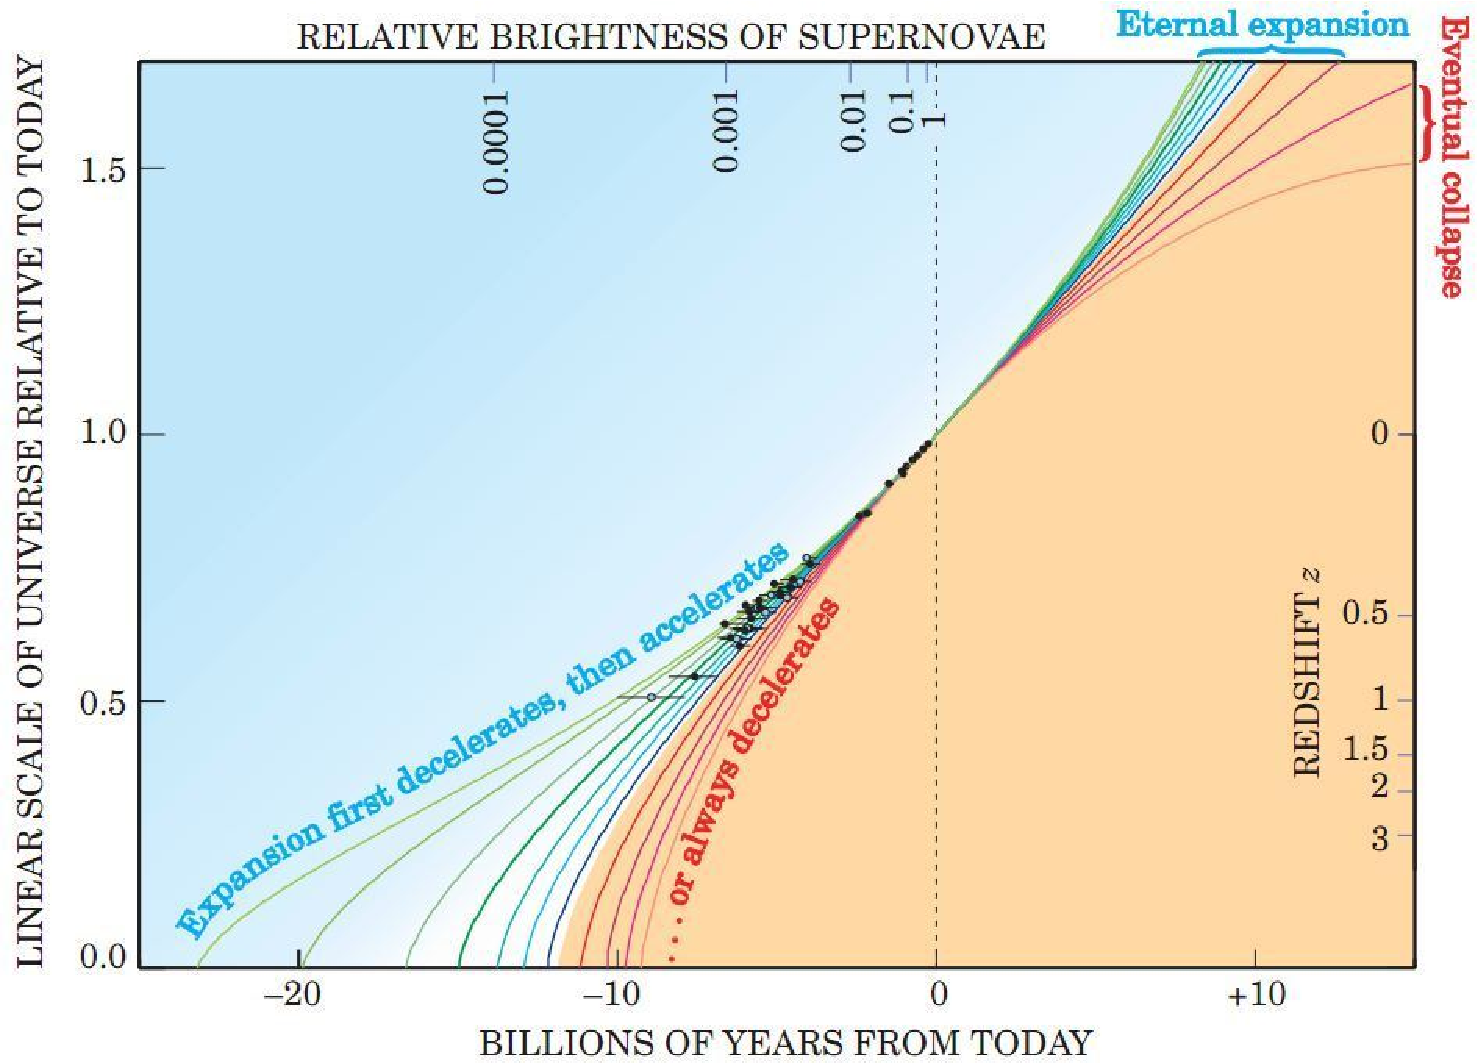
\includegraphics[width=0.8\textwidth]{figure/Scale_Factor_vs-Time.pdf}
  \caption{Andamento $R=R(t)$}
  \label{fig:Rvst}
\end{figure}

Vediamo come sia possibile determinare i parametri di densità $\Omega_i$
attraverso misure di distanza e red-shift.  In effetti, il modo in cui la
costante di Hubble $H(z)$ dipende da $z$ influenza la relazione tra magnitudine
e red-shift.  Preliminarmente osserviamo che dalla definizione $z=R_0/R(t) -1$,
segue
\begin{equation}
  \dd z = -\frac {R_0}{R(t)} H(t) \dd t.
\end{equation}
Consideriamo ora segnali luminosi (per i quali è $d \tau=0$) emessi al tempo $t$
da una galassia che abbia coordinata radiale $r$, e che raggiungono noi (che siamo in
$r=0$) all'istante $t_0$.  Dalla metrica RW si ha
\begin{equation}
  \int_t^{t_0} \frac {\dd t}{R(t)}= \int_0^{r} \frac {\dd r}{\sqrt{1-kr^2}}
  \simeq r + \mathcal{O}(r^3),
\end{equation}
Si ha quindi
\begin{equation}
  r \simeq \int_0^z \frac{\dd z}{R_0 ~ H(t)}.
\end{equation}
La distanza di luminosità $d_L = r R_0 (1+z)$ diventa allora
\begin{equation}
  \begin{split}
    d_L(z) & = (1+z) \int_0^z \frac{\dd z}{H(z)} = \\
           & = (1+z) \int_0^z \frac{\dd z}{H_0
             \left[\Omega_{\Lambda}+\Omega_{k}(1+z)^2+\Omega_m
               (1+z)^3\right]^{1/2}}.
  \end{split}
\end{equation}
Quindi a parità di $z$, gli oggetti osservati (di stessa magnitudine assoluta
$M$) appaiono più o meno lontani a seconda del valore dei parametri cosmologici
(vedere Fig. \ref{fig:Par_Cosm} dove per le supernovae \footnote{In sistemi
  binari di una nana bianca ed una gigante rossa, la massa espulsa dalla gigante
  rossa cade sulla nana bianca, che esplode in supernova quando la sua massa
  supera la massa limite di Chandrasekar. Si ritiene che queste supernovae
  abbiano la stessa luminosità intrinsceca, indipendentemente dalla distanza.}
di tipo Ia (??per la presenza o assenza di particolari righe??) è mostrata la
distanza $d_L$ in funzione del red-shift $z$).  È evidente allora che lo studio
del diagramma $m-z$ per questi oggetti (sufficientemente lontani) permette di
determinare i valori dei parametri $\Omega_{\Lambda}$, $\Omega_{k}$ ed
$\Omega_{m}$.
% In particolare si ha $\Omega_m = 0.27$ ed $\Omega_{\Lambda} =0.73$, se si
% assume $\Omeka_k=0$, il che è dedotto dall'analisi delle anisotropie della
% temperatura della CMB.%


Ricordiamo che per i modelli di Friedmann, la relazione $d_L=d_L(z)$ era
\begin{equation}
  d_L = \frac {1}{H_0} \left[ z+ \frac{1}{2}(1-q_0)z^2\right].
\end{equation}

Questo programma è stato realizzato prendendo come indicatori di distanza le
supernovae di tipo Ia~\parencites{1998AJ....116.1009R}{1999ApJ...517..565P}
\begin{figure}
  \centering
  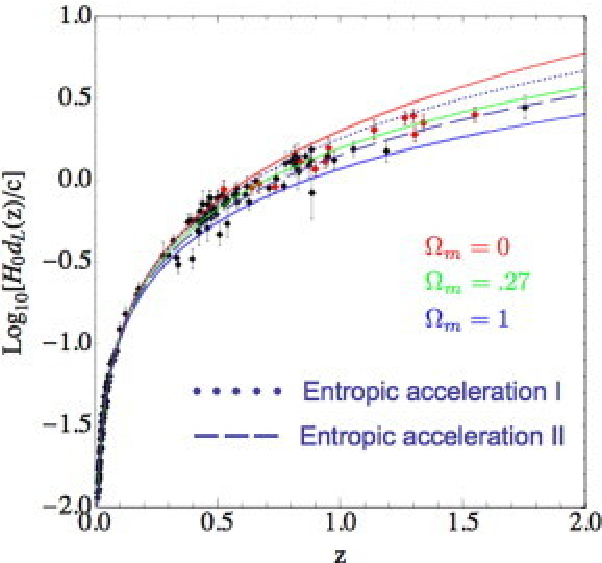
\includegraphics[width=0.8\textwidth]{figure/Hubble_Diagr_1_SNIa.pdf}
  \caption{Diagramma di Hubble SNIa}
  \label{fig:DHSN1}
\end{figure}
% \begin{figure}
%   \centering
%   \includegraphics[scale=1.2]{figure/Hubble_Diagr_2_SNIa.pdf}
%   \caption{Diagramma di Hubble SNIa.}
%   \label{fig:DHSN2}
% \end{figure}
e unitamente all'analisi di dati relativi all'anistrotropia della temperatura
della CMB e della funzione di correlazione angolare di galassie, si sono
determinati i seguenti valori
\begin{subequations}
  \begin{align}
    \Omega_k &= 0, \\
    \Omega_{\Lambda} &\simeq 0.7, \\
    \Omega_{m} &\simeq 0.3.
  \end{align}
\end{subequations}
La figura~\ref{fig:Par_Cosm} mostra che nello spazio dei parametri cosmologici
vi sono tre differenti regioni permesse --- quelle che danno $\chi^2<1$ --- la
cui intersezione determina la regione di valori permessi.
\begin{figure}
  \centering{}
  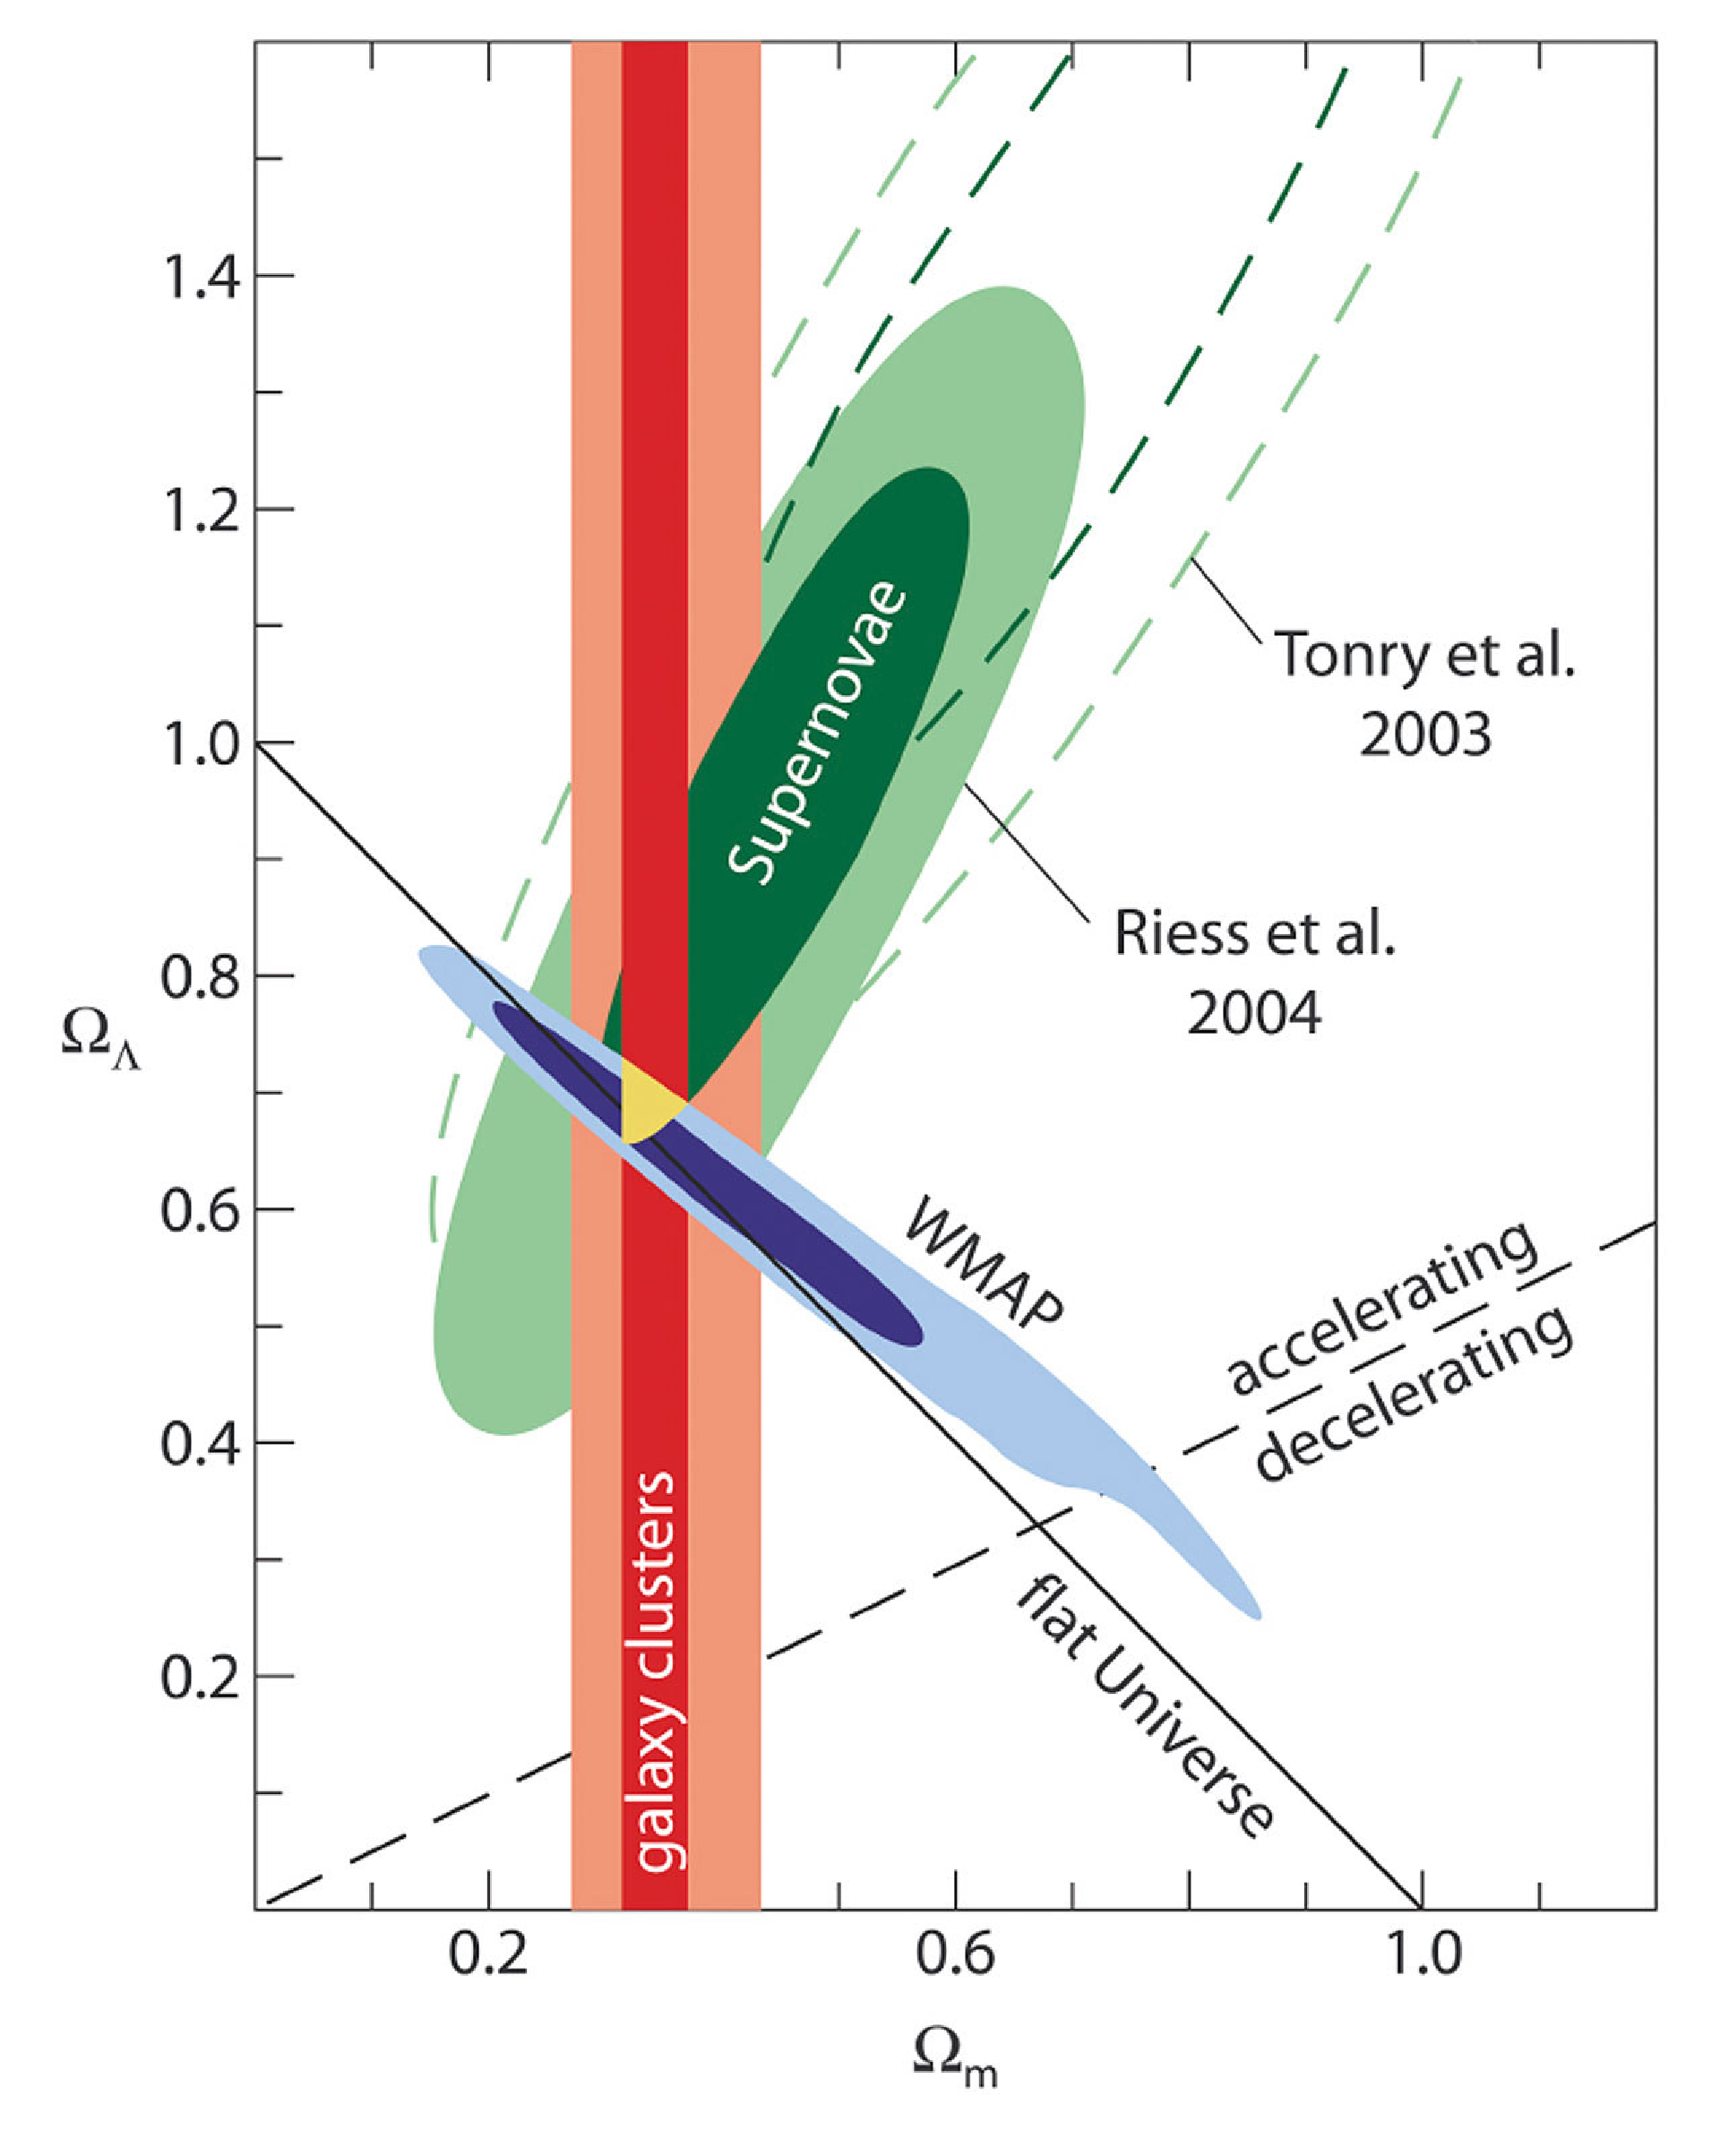
\includegraphics[width=0.6\textwidth]{figure/Cosmological_parameters.pdf}
  \caption{Spazio dei parametri $\Omega_{m}$, $\Omega_{\Lambda}$, $\Omega_k$}
  \label{fig:Par_Cosm}
\end{figure}

\subsubsection{Dark Energy}

Dal punto di vista fenomenologico, invece di introdurre nelle eq. di Einstein (a
sinistra) il termine $g_{\mu \nu}\Lambda$, possiamo introdurre (a destra) un
termine di sorgente con densità $\rho_{DE}$, che attribuiamo ad una nuova
componente dell'Universo nota come Dark Energy.  In generale si assume che la
Dark Energy abbia eq. di stato $p_{DE}=w\rho_{DE}$ con $w<0$.  Il caso $w=-1$
corrispondente alla costante cosmologica.  Ora, se assumiamo che la componente
DE sia disaccoppiata dalla radiazione
\begin{equation}
  \toder{(\rho_{DE} R^3)}{R} = -3 p_{DE} R^2
\end{equation}
si ha
\begin{equation}
  \rho_{DE} \propto \frac {1}{R^{3(1+w)}}
\end{equation}
Pertanto $\rho_{DE}=\text{cost}$ implica $w=-1$ come per il caso
$\rho_{\Lambda}=\text{cost}$, $p_{\Lambda}=-\rho_{\Lambda}$.

Notiamo che il rapporto $\rho_{DE}/\rho_m \propto R^{-3w} \propto (1+z)^{3w}$.
Quindi nel caso $w<0$, per $t < t_0 $ ($z$ crescente a partire dal valore 0), si
ha $\rho_{DE}/\rho_m \to 0$, cioè l'importanza della componente DE diminuisce
indietro nel tempo e i risultati dei modelli di Friedmann non sono modificati
per $z\gg 1$ dalla presenza della componente DE.

L'eq. \eqref{hzcc} risulterà così modificata:
\begin{equation}
  H(z)=H_0 \left[ \Omega_{DE} (1+z)^{3(1+w)} + \Omega_{k} (1+z)^2+ \Omega_m
    (1+z)^3 \right]^{1/2}
  \label{hzccX}
\end{equation}

Anche l'eq. (\ref{ddRcc}) è modificata
\begin{equation}
  \frac {\ddot{R}} {R} = H_0^2
  \left[ - \frac{\Omega_{DE} (1+3w)}{2} (1+z)^{3(1+w)}
    -\frac {\Omega_m (1+z)^3} {2 } \right]
  \label {ddRw}
\end{equation}
da cui per il parametro di decelerazione si ha ora
\begin{equation}
  q_0= \frac{\Omega_{DE}}{2} (1+3w) +  \frac{\Omega_m}{2} + \Omega_{k}
\end{equation}
e, nel caso $k=0$ (poichè $\Omega_m = 1 - \Omega_{DE}$), si ha
\begin{equation}
  q_0= \frac {1+3w \Omega_{DM}}{2},
\end{equation}
per cui se poniamo $\Omega_{DE} \simeq 0.7$ si ha $q_0 =0.5+w$ che diventa
negativo (quindi l'Universo oggi è in una fase di espansione accelerata) se
$w<-0.5$.  In realtà lo studio dei diagramma di Hubble $m-z$ non permette una
precisa determinazione del valore di $w \simeq -0.7$ a causa delle larghe
incertezze dei dati osservativi.

%Tornando indietro alla relazione $d_L(z)$ osserviamo che nel caso $\Omega_{k}=0$
%ed $\Omega_{\Lambda}=0$
%\begin{equation}
%d_L =
%\end{equation}
%mentre se prendo $\Omega_{k}=0$ ed  $\Omega_{m}=0$
%\begin{equation}
%d_L = (1+z) \int_0^z \frac{dz}{H_0 (1+z)^{3(1+w)/2}}
%\end{equation}
%e per $w=-1$ segue $d_L=H_0^{-1} z (1+z)$. Quindi a parità di $z$ oggetti
%appaiono più o meno distanti a seconda del valore dei parametri cosmologici
%$\Omega$.  Vedi figura da cui si ottiene (assumendo $k=0$ $\Omega_{m}=0.32$ ed
%$\Omega_{\Lambda}=0.68$)

L'introduzione della costante cosmologica nelle eq. di Einstein
può essere interpretata in due modi:
\begin{itemize}
\item nel primo caso è come se la lagrangiana della materia sia modificata con
  l'aggiunta di un termine costante
  \begin{equation}
    L_{\textup{matter}} \to L'_{\textup{matter}} = L_{\textup{matter}} -
    \frac{\Lambda}{8 \pi G},
  \end{equation}
  così che l'integrale d'azione diventa
  \begin{equation}
    S_{tot}=S_{g}+S_{m}= \frac {1}{16 \pi G} \int R \sqrt{-g} \dd^4x + \int
    \left( L_{m}- \frac {\Lambda}{8 \pi G} \right) \sqrt{-g} \dd^4 x.
  \end{equation}
  L'eq. del moto per la materia (descritta dal campo $\phi$) che sono ottenute
  variando $S$ rispetto $\phi$ e ponendo $\delta S/\delta \phi=0$, rimangono
  inalterate poiché $\Lambda=\text{cost}$.  In questo caso l'introduzione del
  termine $\Lambda$ introduce solamente uno shift nel livello zero dell'energia
  della materia e non influenza la dinamica della materia, mentre la gravità che
  è accoppiata alla energia totale del sistema ne è influenzata;
\item il secondo caso corrisponde ad un integrale d'azione scritto come
  \begin{equation}
    S_{tot}= \frac {1}{16 \pi G}
    \int (R-2\Lambda)  \sqrt{-g} \dd^4x + \int  L_{m} \sqrt{-g} \dd^4 x,
  \end{equation}
  e la gravità risulta descritta dalle due costanti $G$ e $\Lambda$.  In questo
  secondo caso lo spazio-tempo è curvo anche in assenza di materia.
\end{itemize}

L'eq. di stato $\rho=-p$ ha un'altra importante implicazione in relatività
generale.  La parte spaziale $\bm{g}$ dell'accelerazione geodetica (che misura
l'accelerazione di due particelle di prova molto vicine) soddisfa l'eq.
\begin{equation}
  \nabla \cdot \bm{g} = - 4 \pi G (\rho+3p)~,
\end{equation}
per cui la causa dell'accelerazione geodetica è $\rho+3p$.  Quindi se
$\rho+3p<0$, la gravità diventa repulsiva.

Questo starebbe accadendo oggi nell'Universo poichè all'istante attuale la DE
domina ($\rho_{\Lambda}+3 p_{\Lambda} <0$).  La transizione dalla gravità
attrattiva (dovuta alla materia ordinaria) a quella repulsiva avverrebbe a un
red-shift $\simeq 0.5$.

Quanto vale $\Lambda$?  Preliminarmente osserviamo che $\Lambda$ ha dimensioni
cm$^{-2}$.  La velocità della luce e l'istante attuale $t_0$ definiscono una
lunghezza caratteristica (raggio visibile dell'Universo nel caso $k=1$) $l_0 = c
t_0 \simeq c/H_0 \simeq 10^{28}$ cm $\simeq$3 Gpc.  Poiché l'Universo appare
omogeneo ed isotropo su questa scala (non vi sono effetti indotti da $\Lambda$
nella distribuzione di sorgenti) $\Lambda < 10^{-56}$ cm$^{-2}$.

\section{Radiazione di fondo cosmico}

La radiazione di fondo cosmico nella banda delle microonde (CMB) ha uno spettro
di corpo nero a $T_{CMB}(0) \simeq 2.725$K.  Nella Figura~\ref{fig:radio-gamma}
lo spettro della radiazione extragalactica è mostrato in funzione dell'energia
dei fotoni.  La CMB contribuisce con il 93\% dell'emissione totale.  Definita la
grandezza $f_{\lambda}= \rho_{\lambda}/\rho_{tot}$, si ha:
$f_{CMB}=0.93,$ $f_{IR}= 0.05$, $f_{VIS}=0.02$, $f_{X}=2.5
\times 10^{-4},$ $f_{\gamma}= 2.5 \times 10^{-5}$, $f_{CR} \simeq
\Omega_{CMB}$.
\begin{figure}
  \centering{}
  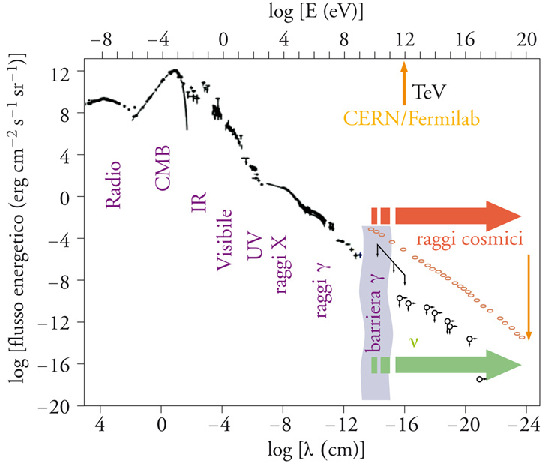
\includegraphics[width=0.8\textwidth]{figure/Radiazione_radio_gamma.pdf}
  \caption{Radiazione dal radio al gamma}
  \label{fig:radio-gamma}
\end{figure}
\begin{figure}
  \centering{}
  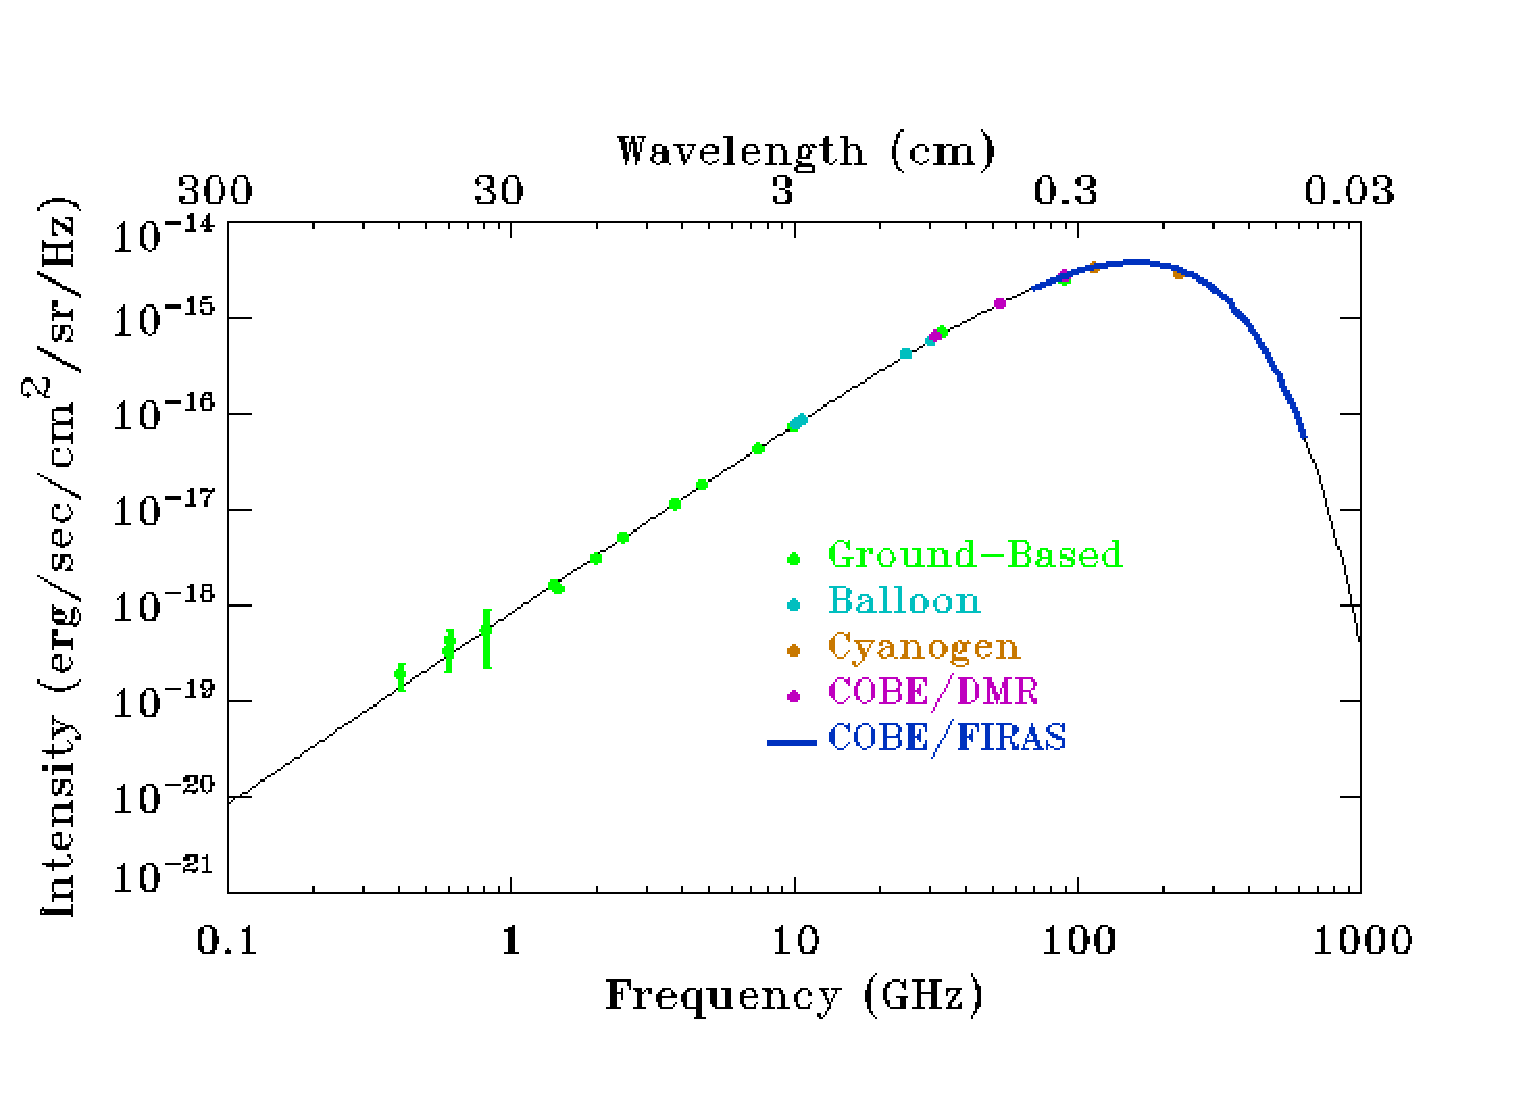
\includegraphics[width=\textwidth]{figure/CMB_intensity.pdf}
  \caption{CMB e distribuzione di Planck a $T_{CMB} = 2.75$K}
  \label{fig:spettro_CMB}
\end{figure}
La densità di energia di un gas di bosoni è
\begin{equation}
  d \rho (p)  = g \frac{4 \pi p^2 dp} {h^3} \frac{1} {\exp[ E(p) / kT ]-1} E(p)
\end{equation}
e poichè (i fotoni sono bosoni di massa nulla) $E(p)=pc=h\nu$ e $g=2$, si ha
\begin{equation}
  d \rho_{\gamma}(\nu) =   \frac{8 \pi h \nu^3 } {c^3} \frac{1} {\exp(h \nu/ kT)
    -1} d\nu
  \label{spettro_BB}
\end{equation}

Posto $x=(h \nu/kT)$, nello spettro di corpo nero si distingue la regione di
Rayleigh-Jeans (con $x\ll 1$) in cui lo spettro cresce come $x^2$ e la regione
di Wien con spettro decrescente come $x^3 \exp(-x)$.  Il massimo dello spettro
si trova derivando l'eq.  \eqref{spettro_BB} rispetto ad $x$ e uguagliando a
zero.  Si ottiene $3(\exp x_{max} -1) = x_{max} \exp(x_{max})$, che ha soluzione
numerica $x_{max} \simeq 2.8$. Quindi $(h \nu_{max}) \simeq 2.8 kT_{max}$, da
cui $(h \nu_{max}) \simeq 2.4 \times 10^{-4}$ eV o, equivalentemente,
$\lambda_{max} \simeq 1.7$ mm, $\nu_{max} \simeq 1.8 \times 10^{11}$ Hz.

La densità totale di energia si calcola integrando lo spettro su tutte le
frequenze
\begin{equation}
  \begin{split}
    \rho_{\gamma}(t_0) &= \int_0^{\infty} \frac{8 \pi h \nu^3 } {c^3}
    \frac{\dd\nu} {\exp (h \nu/
      kT_0) -1} \\
    &= \frac{8 \pi k^4 T^4_0}{c^3 h^3} \int_0^{\infty} \frac{x^3}{e^{x} -1} \dd
    x \\
    & = a T^4_0 \\
    & = 4.64 \times 10^{-34}~~{\rm gr~cm^{-3}} \implies \Omega_{\gamma} =2.47
    \times 10^{-5} h^{-2}
\end{split}
\end{equation}
dove $a=(8 \pi k^4)/(15 h^3 c^3) = 7.56 \times 10^{-15}$ erg cm$^{-3}$
deg$^{-4}$ è la costante di Stefan-Boltzmann, e $h$ è la costante di Hubble in
unità di $100$ km/sec/Mpc, cioè $h=H_0/100$ km/sec/Mpc.

La densità spaziale di fotoni della CMB all'istante attuale è
\begin{equation}
  \begin{split}
    n_{\gamma}(t_0) & = \int_0^{\infty} \frac{\rho_{\gamma}(t_0) } {h \nu }
    \dd\nu
    = \frac{8 \pi k^3 T^3_0 }{c^3 h^3} \int_0^{\infty} \frac{x^2}{e^x -1} \dd x
    \\
    & = \frac{30 a \zeta(3) T^3_0} {\pi^4 k} = 0.3702 \frac{a T^3_0}{k} = 410
    ~{\rm fotoni/cm^3}
  \end{split}
\end{equation}
L'attuale  densità di nucleoni  è invece
\begin{equation}
  n_N (t_0) = \frac{3 \Omega_B H_0^2}{8 \pi G m_N c^2} =
  1.123 \times 10^{-5} \Omega_B h^2 ~{\rm nucleoni/cm^3}
\end{equation}
e il rapporto tra le due densità rimane costante nel tempo (perché entrambe
variano come $\propto R^{-3}$)
\begin{equation}
  \frac{n_{\gamma}(t_0)}{n_N(t_0)} = 3.65 \times 10^{7}.
\end{equation}

A temperature $T>4000~$K l'Universo è opaco alla radiazione con $\gamma$, H$^+$,
e$^-$ in contatto termico alla stessa temperatura e $\gamma$ con spettro di
corpo nero; a $T \simeq 4000$K si forma l'idrogeno neutro e l'Universo diventa
trasparente alla radiazione, nel senso che l'assorbimento di un fotone alla
frequenza $\nu= \Delta E/h$ è seguito da emissione isotropa di un fotone alla
stessa frequenza.

Ma lo spettro continua ad essere di corpo nero. Per dimostrarlo, supponiamo che
la transizione tra Universo opaco e Universo trasparente avvenga istantaneamente
al tempo di ultimo scattering $t_{LS}$ a cui la temperatura ha il valore
$T_{LS}$.

Se consideriamo tempi successivi $t>t_{LS}$ abbiamo le seguenti proprietà
\begin{itemize}
\item fotoni che al tempo $t$ hanno frequenza $\nu$, a $t_{LS}$ avevano
  frequenza (maggiore) $\nu R(t)/R(t_{LS})$
\item a causa dell'espansione la densità propria di fotoni diminuisce come
  $[R(t_{LS})/R(t)]^3$.
\end{itemize}
Quindi, al tempo $t$ la densità di fotoni con frequenza tra $\nu$ e $\nu+d\nu$ è
determinata a partire dalla densità al tempo $t_{LS}$ modificata dalle proprietà
precedenti:
\begin{equation}
  n_{\gamma}(\nu, t) d\nu = \left( \frac {R(t_{LS})} {R(t)} \right)^3
  8 \pi \nu^2 d \nu
  \left( \exp \left[ \frac {h} {k T_{LS}} \frac{\nu R(t)}{R(t_{LS})} \right] -1
  \right)^{-1} \left( \frac {R(t)} {R(t_{LS})} \right)^3
\end{equation}
da ciò si vede che $n_{\gamma}(\nu,t)$ è una distribuzione di corpo nero a ogni
$t$ se
\begin{equation}
  T(t) = T_{LS} \frac {R(t_{LS})} {R(t)}
\end{equation}

Questa conclusione è inalterata se la transizione dall'opacità alla trasparenza
avviene in un tempo finito poichè l'interazione $\gamma H$ è limitata allo
scattering elastico per il quale le frequenze dei $\gamma$ non cambiano.

Dopo il disaccoppiamento tra materia e radiazione si ha $\rho_{\gamma} \propto
R^{-4}$ e poiché $\rho_{\gamma} \propto T^4$, si ha $T_{\gamma} \propto
R(t)^{-1}$.  Ma prima del disaccoppiamento come varia la temperatura dei fotoni
in contatto termico con la materia?  A questo scopo consideriamo un semplice
modello per l'Universo che supponiamo costituito da un gas ideale e radiazione
alla stessa temperatura $T_{\gamma}=T_{m}=T$. Densità e pressione delle due
componenti sono
\begin{subequations}
  \begin{align}
    \rho_{\gamma} & = a T^4 \\
    p_{\gamma} &=\rho/3  \\
    \rho_{m}    & = n_N m c^2 + \frac{p_{m}}{\gamma-1} \\
    p_m &=n_N kT
  \end{align}
\end{subequations}
dove l'indice politropico $\gamma=5/3$ $(4/3)$ per il regime non relativistico
(relativistico).  Per la densità e pressione totali avremo $\rho =
\rho_{m}+\rho_{\gamma}$ e $p=p_{m}+p_{\gamma}$ e sostituendo
nell'eq. \eqref{moto} si trova l'eq. differenziale
\begin{equation}
  \label{TvsR}
  \frac{R}{T} \toder{T}{R} = -
  \left(\frac{\sigma+1}{\sigma+[3(\gamma-1)]^{-1}}\right)
\end{equation}
dove la costante $\sigma = 4 a T^3_{\gamma}/(3 n_N k)$ è l'entropia specifica.  Ora:
\begin{itemize}
\item se $\sigma \ll 1$, dall'eq. \eqref{TvsR} segue $T \propto
  R^{-3(\gamma-1)}$ che è l'usuale relazione temperatura-volume per
  un'espansione adiabatica di un gas ideale, e infine
  $T \propto R^{-1}$ nel caso relativistico (per cui $\gamma=4/3$)
e $ T \propto R^{-2}$ nel caso non-relativistico (per cui $\gamma=5/3$);
\item se $\sigma \gg 1$ si ha sempre $T \propto R^{-1}$.
\end{itemize}

Nel nostro caso $\sigma = 4 a T^3_{\gamma}(0)/(4 n_N(0) k) \simeq 10^8$ e quindi
prima del disaccoppiamento la materia (nonostante sia in un regime
non-relativistico) segue la radiazione con $T_m=T_{CMB} \propto R^{-1}$.  Dopo
il disaccoppiamento la temperatura della materia $T_{m}\propto R^{-2}$.

\subsection{Anisotropia di dipolo}

Supponiamo che vi sia un sistema di riferimento fondamentale in cui la
radiazione di fondo cosmico sia isotropa (e con spettro di Planck) e che la
Terra si muova con velocità $v_{\oplus}$ rispetto a questo sistema.  Nel sistema
fondamentale, i fotoni nell'angolo solido $\sin \theta \dd \theta \dd \phi$ e
con frequenza tra $\nu$ e $\nu + \dd\nu$ contribuiscono al tensore energia
impulso della radiazione di fondo cosmico con
\begin{equation}
  \dd T^{\mu \nu}=  \left( \frac{p^{\mu} p^{\nu}}{h^2 \nu^2} \right)
                  \left( \frac{\sin\theta \dd\theta \dd\phi}{4\pi} \right)
  \rho_{\gamma 0}(\nu) \dd\nu
\label{521}
\end{equation}
Nella relazione precedente si è tenuto conto che il tensore energia impulso è
proporzionale a $p^{\mu} p^{\nu}$ (vedi~\cite[44]{weinberg:gravitation}); gli
altri termini sono introdotti in modo che integrando sull'intero angolo solido
$\dd T^{00} = \rho_{\gamma 0} \dd \nu$.  Si ha quindi
\begin{equation}
  \dd T^{\mu \nu}= \left( 2 \frac{ p^{\mu} p^{\nu} }{h} \right)
                   \left( \frac{1} { \exp (h \nu/ kT_{\gamma 0 }) } \right)
  \sin \theta \dd\theta \dd\phi \nu \dd\nu
\label{522}
\end{equation}
con
\begin{equation}
  p^{\mu} \equiv (E, p_x, p_y, p_z) =
  h \nu ( 1, \sin \theta \cos \phi , \sin \theta \sin \phi, \cos \theta)
\end{equation}

Nel sistema della Terra il tensore energia impulso della radiazione di fondo è
\begin{equation}
  \dd T'^{\mu \nu} = \tensor{\Lambda}{^{\mu}_{\rho}} \tensor{\Lambda}{^{\nu}_{\sigma}}
  \dd T^{\rho\sigma}
\end{equation}
dove $\Lambda$ è la matrice di Lorentz con $\vec{v} = - \vec{v}_{\oplus}$.
Allora possiamo esprimere $\dd T'^{\mu \nu}$ in termini di quantità nel sistema
della Terra.  Osserviamo preliminarmente
\begin{equation}
  p'^{\mu } = \tensor{\Lambda}{^{\mu}_{\nu}} p^{\nu}
\end{equation}
e che orientando gli assi in modo ($\phi=0$) che l'asse z sia nella direzione della
velocità della Terra,  si ha
\begin{subequations}
  \begin{gather}
    \nu' = \nu \frac{[1-v_{\oplus}\cos\theta]}{[ 1 - v_{\oplus}^2]^{1/2}}, \\
    \cos\theta' = \frac{[- v_{\oplus} + \cos\theta]}{[1 - v_{\oplus}
      \cos\theta]}, \\
    \phi' = \phi
  \end{gather}
\end{subequations}
dove ora $\theta$ è l'angolo tra la velocità della Terra e il fotone.
Il tensore energia impulso differenziale nel sistema terra ha necessariamente la forma
\begin{equation}
  \dd T^{\prime \mu \nu}= \left( 2 \frac{ p^{\prime \mu} p^{\prime \nu} }{h} \right)
                   \left( \frac{1} { \exp (h \nu/ kT_{\gamma 0 }) } \right)
  \sin \theta \dd\theta \dd\phi \nu \dd\nu
\end{equation}
poiché in eq.~\eqref{522} il termine a sinistra è un tensore di rango 2
controvariante, il prodotto $p^{\mu} p^{\nu}$ è un tensore dello stesso tipo e
rango e quindi la parte restante a destra è un invariante.  Ora, l'angolo solido
ha la regola di trasformazione (?)
\begin{equation}
 \sin \theta^{\prime} \dd\theta^{\prime} \dd\phi^{\prime}
= \left( \frac {\nu}{\nu^{\prime}} \right)^2 \sin \theta \dd\theta \dd\phi
\end{equation}
da cui segue
\begin{equation}
  \dd T^{\prime \mu \nu}= \left( 2 \frac{ p^{\prime \mu} p^{\prime \nu} }{h} \right)
                   \left( \frac{1} { \exp (h \nu^{\prime}/ kT^{\prime}_{\gamma 0 }) } \right)
  \sin \theta^{\prime} \dd\theta^{\prime} \dd\phi^{\prime} \nu^{\prime} \dd\nu^{\prime}
\end{equation}
dove si \'e posto
\begin{equation}
T^{\prime}_{\gamma 0} \equiv \left( \frac{\nu ^{\prime}}{\nu} \right) T_{\gamma 0} =
\left[ \frac{(1- v_{\oplus} \cos \theta)}{(1-v_{\oplus}^2)^{1/2} } \right] T_{\gamma 0}
\end{equation}
Quindi, rispetto alla Terra la radiazione di fondo cosmico ha ancora una distribuzione di Planck
ma con una temperatura differente.
Per velocit\'a piccole, cio\'e per $v_{\oplus}/c << 1$, segue che
\begin{equation}
\Delta T_{\gamma 0} = T^{\prime}_{\gamma 0} - T_{\gamma 0} = - \frac{ v_{\oplus}} {c} T_{\gamma 0}
\end{equation}
Questa relazione determina un'anisopropia di dipolo in due direzioni opposte.
Da misure recenti si trova $v_{\oplus} \simeq 300$ km/s (nel direzione ....) e quindi
$  \Delta T_{\gamma 0} / T_{\gamma 0} \simeq 10^{-3}$.

\subsection{Effetto GZK}

I raggi cosmici, prevalentemente protoni, sono prodotti da acceleratori cosmici
(SN galattiche fino ad energia $E_{CR} \simeq 10^{15}$ eV, AGN extragalattici
per energie maggiori) ed hanno uno spettro che si estende da circa $10^9$ ev fino a $10^{21}$ ev
seguendo semplici leggi di potenza. (Vedi Fig. \ref{fig:CR1})
 \begin{figure}
   \centering{}
   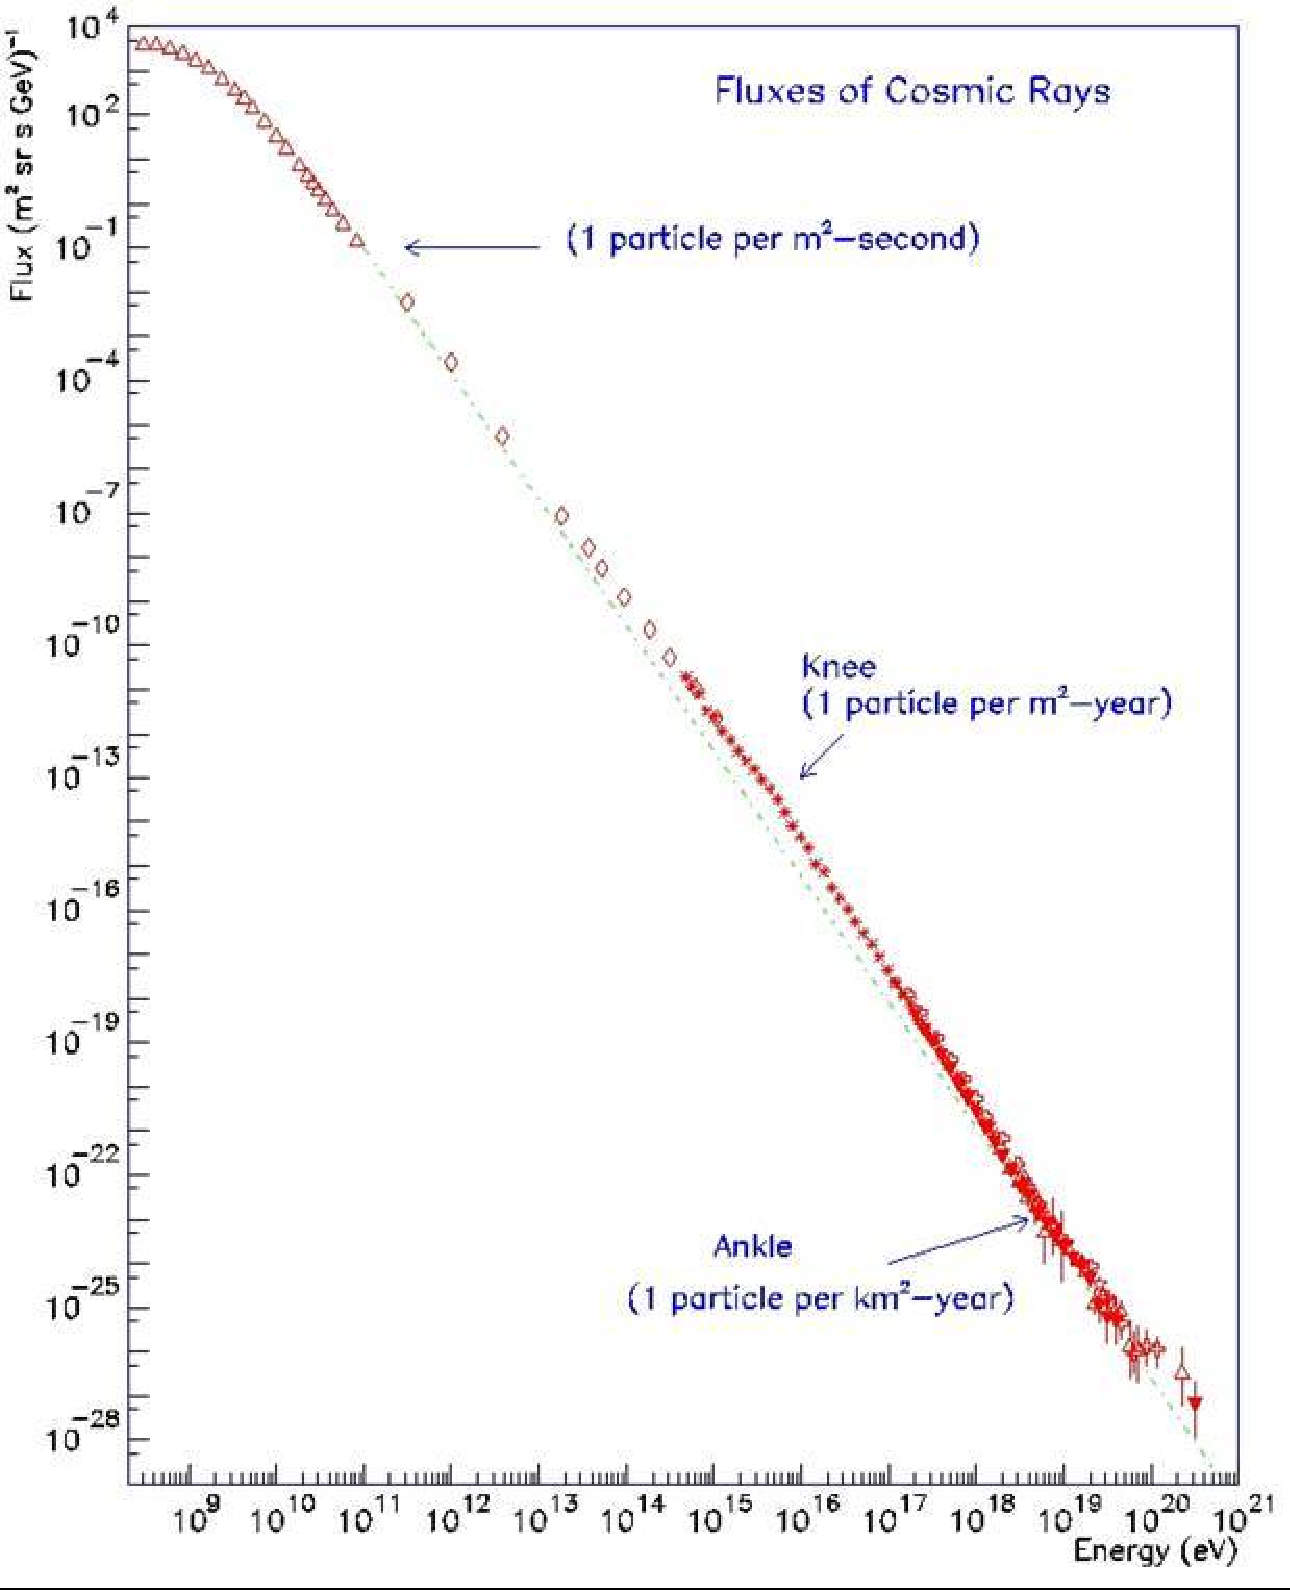
\includegraphics[width=0.8\textwidth]{figure/CR_spectrum_1.pdf}
  \caption{Spettro dei Raggi Cosmici}
  \label{fig:CR1}
\end{figure}
Comunque ad energie $E_{CR} \simeq 10^{20}$ eV si osserva nello spettro dei CR
una perdita di flusso che è una dimostrazione indiretta dell'esistenza della
CMB: protoni di alta energia interagiscono con i fotoni del fondo cosmico dando
luogo ad interazioni forti del tipo $p \gamma_{CMB} \to p \pi^0$ e $\gamma_{CMB}
p \to n \pi^+$, e quindi non ci raggiungono.  Tali processi, comunque, avvengono
attraverso la creazione di risonanze (stati metastabili intermedi)
$\Delta^{++}$, $\Delta^{+}$, $\Delta^{0}$ e il loro successivo decadimento.
L'effetto è stato predetto
da~\textcites{1966PhRvL..16..748G}{1966JETPL...4...78Z}.

La massa della risonanza $m_{\Delta} \simeq 1236$ MeV pone un limite inferiore
all'energia dei protoni dei CR capaci di attivare il processo di annichilazione.
Consideriamo la cinematica del processo.  Nel sistema del laboratorio sia
\begin{subequations}
  \begin{align}
    P^{\mu}_{\gamma}       &= (q, \bm{q}), \\
    P^{\mu}_{\ \textup{p}}   &= (\sqrt{p^2+m^2_\textup{p}}, \bm{p}), \\
    P^{\mu}_{\ \textup{tot}} &= ( q+\sqrt{p^2+m^2_\textup{p}}  ,  \bm{q} + \bm{p}) \\
    \sqrt{s} &= \sqrt{ P^{\mu}_{\ \textup{tot}} P_{\mu \ \textup{tot}} } =
                        \left[ \left( q+\sqrt{p^2+m^2_\textup{p}} \right)^2 -
                        \left(\bm{q}+ \bm{p} \right)^2 \right]^{1/2} \\
                      & \simeq \left[ 2qp \left(1-\cos \theta \right) +
                        m_\textup{p}^2 \right]^{1/2}.
  \end{align}
\end{subequations}
La reazione può avvenire se $\sqrt{s} > m_{\Delta} c^2$.  La tipica energia
$\langle E_{\gamma}\rangle$ dei fotoni della CMB è $6 \times 10^{-4}$ eV e il
massimo di $(1-\cos \theta)=2$.  Si ha quindi
\begin{equation}
  p_{\textup{th}} \simeq \frac{m^2_{\ \Delta} c^4 - m^2_{\ p} c^4} {4 \langle
    \ E_{\gamma}\rangle} \simeq 10^{20}~~~{\rm eV}
\end{equation}
Nella figura~\ref{fig:CR2} è riportato lo spettro dei raggi cosmici attorno al
taglio GZK.
\begin{figure}
  \centering{}
  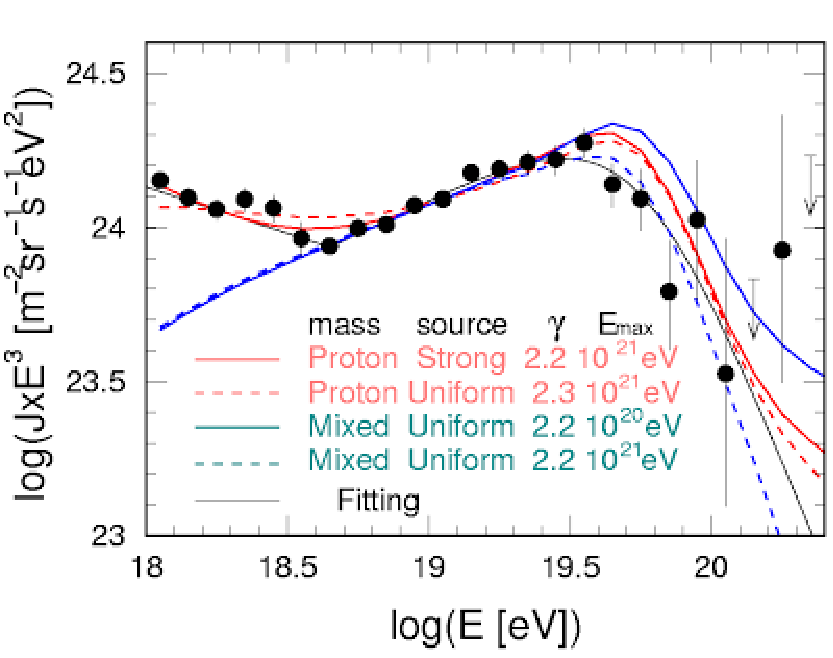
\includegraphics[width=\textwidth]{figure/CR_spectrum_2.pdf}
  \caption{Spettro dei Raggi Cosmici a $E \simeq 10^{20}$ eV}
  \label{fig:CR2}
\end{figure}

\section{Conservazione dell'entropia}

Si consideri un gas perfetto con densità e pressione $\rho= \rho(T)$ e $p=p(T)$.
Le leggi della termodinamica sono
\begin{subequations}
  \label{leggi_termo}
  \begin{align}
    \dd Q &= \dd U+p\dd V \\
    \dd S &= \frac{\dd Q}{T}
  \end{align}
\end{subequations}
in cui $dQ$ è il calore assorbito, $dU=d(\rho c^2 V)$ la variazione di energia
interna, $pdV$ il lavoro eseguito, $dS$ la variazione di entropia, $V$ infine è
il volume occupato dal gas.

Dalle leggi della termodinamica si ha
\begin{equation}
  \begin{split}
    \dd S &=  \frac{1}{T} \left( \dd( \rho c^2 V) + p \dd V \right) \\
    &= \frac{1}{T} \left( V \dd(\rho c^2) + (\rho c^2+p) \dd V \right) \\
    &= \frac{1}{T} \left( V \toder{(\rho c^2)}{T} \dd T + (\rho c^2+p) \dd V
    \right).
  \end{split}
\end{equation}
Poichè $S=S(V,T)$ segue
\begin{equation}
  \dd S = \left( \frac{\partial S}{\partial T} \right)_V \dd T +
  \left( \parder{S}{V} \right)_T \dd V
\end{equation}
dal confronto tra le precedenti eq. si ha
\begin{subequations}
  \begin{align}
    \left(\parder{S}{V}\right)_T &= \frac{1}{T} (\rho c^2+p) \\
    \left(\parder{S}{T}\right)_V &= \frac{V}{T} \toder{(\rho c^2)}{T}.
  \end{align}
\end{subequations}
La condizione di integrabilità
\begin{equation}
  \frac{\partial}{\partial T} \left( \frac{\partial S}{\partial V} \right) =
  \frac{\partial}{\partial V} \left( \frac{\partial S}{\partial T} \right)
\end{equation}
conduce alla relazione
\begin{equation}
  \toder{p}{T} = \frac{1}{T} (\rho c^2 +p).
  \label{integrab}
\end{equation}
Usando questa relazione nella legge di conservazione dell'energia \eqref{moto}
si ha
\begin{equation}
  \begin{split}
    \toder{}{t} [R^3(\rho c^2 +p)] & = R^3 \toder{p}{t} \\
    & = R^3 \toder{p}{T} \toder{T}{t} \\
    & = R^3 (\rho c^2 +p) \frac{1}{T} \toder{T}{t}
  \end{split}
\end{equation}
da cui segue
\begin{equation}
  \toder{}{t} \left( \frac{R^3}{T} (\rho c^2 + p) \right) = 0.
\end{equation}
Se indichiamo con $S(t)$ l'entropia contenuta nel volume comoving, abbiamo
\begin{subequations}
  \begin{align}
    S(t) & =  \left( \frac{R^3}{T} (\rho c^2 + p) \right) \\
    \toder{S(t)}{t} & = 0 \iff S(t)= \text{cost}
  \end{align}
  \label{cons_entropia}
\end{subequations}
che esprime la conservazione dell'entropia contenuta in un volume comoving (che
scala come $R^3$).

Verifichiamo che la definizione di $S$ è consistente con la $2^a$ legge della
termodinamica in eq. \eqref{leggi_termo}, che riscriviamo nella forma
\begin{equation}
  \dd S  = \frac{1}{T} \left( \dd(\rho c^2 V) + \dd(pV) - V \toder{p}{T} dT
  \right)
\end{equation}
e usando l'eq. \eqref{integrab}
\begin{equation}
  \begin{split}
    \dd S &= \frac{1}{T} \left( \dd(\rho c^2 V + pV) -  \frac{V}{T}   (\rho c^2
      +p) \dd T \right) \\
    &= \dd\left( \frac{V (\rho c^2 + p)} {T}  \right)
  \end{split}
\end{equation}
che è la relazione in eq. \eqref{cons_entropia} poiché $V \propto R^3$.

\section{Universo primordiale}

Si prende ora in esame l'era dell'Universo dominata dalla radiazione, per cui
\begin{equation}
  \rho(t)=\rho_0 \left(\frac{R_0}{R(t)} \right)^4
  \label{293}
\end{equation}
La dinamica dell'Universo è descritta dall'eq. \eqref{eq:friedmann}, in cui ora
però si può trascurare il termine $k$
\begin{equation}
  \dot{R}^2 = \frac{8 \pi G}{3} \rho R^2,
  \label{fri_pri}
\end{equation}
in quanto il termine $(8 \pi G /3) \rho R^2$ risulta essere $\gg 1$ nell'era
della radiazione.  Infatti, all'istante attuale $t_0$ si ha
\begin{equation}
  \frac{8 \pi G}{3} \rho_0 R^2_0 = \frac{2q_0}{|2q_0-1|} > 0.03
\end{equation}
poichè $q_0>0.014$.  D'altra parte indietro nel tempo, tale termine cresce
almeno come $z$ e quando $z\simeq 1000$ (inizio era radiazione) risulta $>30$.

Da eq. \eqref{293} e \eqref{fri_pri} si ha
\begin{equation}
  \frac{\dot \rho}{\rho} = -4 \frac{\dot R}{R} = - 4 \left( \frac{8 \pi G
      \rho}{3} \right)^{1/2}
\end{equation}
da cui segue la relazione tra $t$ e $\rho$
\begin{equation}
  t = \left( \frac{3}{32 \pi G \rho} \right)^{1/2} + \text{cost}\ .
  \label{tvsrho}
\end{equation}

L'obiettivo ora è quello di ricavare $\rho= \rho(T)$.  Ovviamente ci riferiamo
ad un era in cui le galassie non si erano ancora formate ed il fluido
cosmologico è diffuso con densità (quasi) uniforme.  In realtà all'interno della
materia (prevalentemente dark) e della radiazione sono presenti (i semi delle
galassie) le fluttuazioni di densità (prodotte da transizioni di fase tra
$10^{-43} - 10^{30} sec$, durante l'epoca inflazionaria) che si accrescono a
causa del meccanismo di Jeans (instabilità gravitazionali di sistemi di
dimensioni maggiori della lunghezza d'onda di Jeans).  Al disaccoppiamento,
comunque, i contrasti di densità sono ancora molto piccoli, poiché $\Delta \rho
/ \rho \simeq \Delta T / T \simeq 10^{-5}$ durante l'era in cui ci è contatto
termico tra materia e radiazione. I picchi di densità successivamente si
accrescono fino alla creazione di strutture autogravitanti di materia oscura. Si
formano quindi prima sistemi autogravitanti di materia oscura e poi su queste
buche di potenziale gravitazionale cadono i barioni, che attraverso processi
dissipativi, alla fine danno luogo alle strutture visibili ammassi, galassie,
stelle.

A partire dal tempo a cui le interazioni deboli ed elettromagnetiche si sono separate,
$t > 10^{-30}$ secondi, $T < 100 $ Gev, i costituenti dell'Universo vanno ricercati
tra le seguenti particelle:
\begin{itemize}
\item gli adroni = barioni (n,p,..) \& mesoni ($\pi$, k, ...) e rispettive
  antiparticelle;
\item i leptoni = e, $\mu$, $\tau$, $\nu_e$, $\nu_{\mu}$, $\nu_{\tau}$ e
  rispettive antiparticelle;
\item i fotoni,
\end{itemize}
e la composizione del fluido cosmologico ad ogni $T(t)$ è caratterizzata da:
\begin{itemize}
\item particelle di massa $m$ in equilibrio con la radiazione, con $mc^2\ll kT$;
\item particelle di massa $m$ disaccoppiate dalla radiazione, con $mc^2\gg kT$;
\item particelle in transizione con $mc^2 \simeq kT$.
\end{itemize}
Nel primo caso la temperatura dei fotoni è sufficientemente alta così che le
reazioni di creazione e di annichilazione
\begin{equation}
  \text{particella + antiparticella} \to \gamma \gamma
\end{equation}
procedono con la stessa rate nei due sensi.

Nel secondo caso, la temperatura è bassa (rispetto alla massa a riposo) e le
reazioni avvengono prevalentemente nel verso dell'annichilazione, il che produce
rapidamente la scomparsa delle antiparticelle (si ipotizza che l'Universo nasca
con un eccesso di particelle) lasciando alla fine tracce di particelle.


Con riferimento alle masse delle particelle e alla relazione $m c^2 = kT$, si
definisce una scala di temperatura (K$^{-1} = 11604$ Kelvin/eV):
\begin{table}
  \centering{}
  \caption{Corrispondenza $m c^2 = kT$}
  \label{massa_temp}
  \begin{tabular}{ccc}
    \toprule
    T (deg)         & Energia    & T (K)              \\
    \midrule
    $m_n c^2$       & 939.55 MeV & $1.090 \times 10^{13}$ \\
    $m_p c^2 $      & 938.25 MeV & $1.088 \times 10^{13}$ \\
    $m_{\tau}c^2$   & 177    MeV & $2.1   \times 10^{12}$ \\
    $m_{\pi} c^2$   & 140    MeV & $1.6   \times 10^{12}$ \\
    $m_{\mu} c^2 $  & 106    MeV & $1.2   \times 10^{12}$ \\
    $(m_n-m_p) c^2$ & 1.3    MeV & $1.5   \times 10^{10}$ \\
    $m_e c^2      $ & 511    KeV & $5.8   \times 10^{9 }$ \\
    temperatura di dissociazione del deuterio \\
    \bottomrule
  \end{tabular}
\end{table}
in cui si distinguono le seguenti fasi:
\begin{itemize}
\item[(A)] $T \gg 10^{13}$K: tutte le particelle presenti (era adronica);
\item[(B)] $T \simeq 10^{12}$K: gli adroni sono scomparsi; rimangono tracce di
  adroni (n,p) in eccesso rispetto alle antiparticelle inizialmente presenti, e
  tutti leptoni;
\item[(C)] $T < 10^{12}$K: i leptoni pesanti $\mu$ e $\tau$ scompaiono e i
  neutrini $\nu_e$, $\nu_{\mu}$ e $\nu_{\tau}$ disaccoppiano con temperatura
  $T_{\nu}$; il fluido cosmologico è composto da n, p, e$^-$, e$^+$, $\gamma$ in
  equilibrio alla stessa temperatura $T$;
\item[(D)] $T < 10^{11}$K: la differenza di massa tra neutroni e protoni produce
  un eccesso di protoni;
\item[(E)] $T < 5 \times 10^{9}$K: ($t \simeq $ 4 sec dalla singolarità), le
  coppie $\text{e}^- \text{e}^+ \to \gamma \gamma$, lasciando tracce di p, n,
  e$^-$, $\gamma$ in equilibrio ad una temperatura $T > T_{\nu}$ dei neutrini
  già disaccoppiati;
\item[(F)] $T \simeq 10^{9}$K: ($t \simeq 180$ sec) i nuclei di deuterio
  diventano stabili e i neutroni sopravvissuti al decadimento in protoni
  rapidamente si fondono nei nuclei degli elementi leggeri; da questo momento
  fino alla ricombinazione l'Universo è costituito da un plasma ionizzato,
  prevalentemente $H^+$, $^4He^2$ ed elettroni (nella percentuale di 1 atomo di elio per
  ogni 11 atomi di idrogeno), in equilibrio con i $\gamma$, mentre i neutrini
  già disaccoppiati sono a temperatura più bassa;
\item[(G)] tra $(4000 < T < 10^{9})$K: espansione libera con $T_m = T \propto
  R^{-1}$ e $\gamma$ termalizzati (con spettro di corpo nero) fino alla
  ricombinazione;
\item[(H)] tra $(10^3 -10^5)$K, l'Universo entra nell'era della materia.
\end{itemize}

Ricorrendo ai metodi della meccanica statistica è possibile ora esprimere le
densità di energia delle particelle presenti nell'Universo alle varie epoche in
funzione della temperatura.  Infatti, nell'approssimazione di gas perfetto,
fermioni e bosoni sono descritti dalle statistiche di Fermi-Dirac e
Bose-Einstein. Per la specie $i$, la densità in numero di particelle con impulso
tra $q$ e $q+dq$ è
\begin{equation}
  n_i(q) \dd p = \frac{g_i 4 \pi q^2 \dd q} {h^3} \left( \exp\left[{
        {\frac{E(q)-\mu_i}{KT}} }\right] \pm 1 \right)^{-1}
\end{equation}
in cui l'energia $E =(q^2+m^2)^{1/2}$, $\mu_i$ è il potenziale chimico, il segno
$+$ per fermioni, il segno $-$ per bosoni, $g_i$ la molteplicità rispetto allo
spin ($g_i=2 s_i+1$ per particelle di massa $m_i \ne 0$, $g_i=2$ per fotoni e
neutrini).

Con la semplificazione $\mu_i=0$ (particelle e antiparticelle uguali in numero)
ed $E \simeq q$ (tutti i leptoni sono relativistici) si ha:
\begin{subequations}
  \begin{align}
    \rho_{\gamma} & = a T^4 \\
    \rho_e &=\rho_{\mu}=\rho_{\tau} = \frac{7}{8} a T^4 \\
    \rho_{\nu}    & = \frac{7}{16} a T^4.
  \end{align}
\end{subequations}
Queste relazioni permettono di esprimere $\rho$ ad ogni epoca in funzione di $T$
(trascurando le tracce di barioni).

Nell'intervallo di temperatura $(10^{10} < T < 10^{12})$K la densità totale del
fluido cosmologico è
\begin{equation}
  \rho = 2 \left(\rho_{\nu_\textup{e}} + \rho_{\nu_{\mu}} + \rho_{\nu_{\tau}} +
    \rho_{\textup{e}} \right)+\rho_{\gamma}=\frac{43}{8}a T^4
\end{equation}
con neutrini disaccoppiati dal fluido e $T_{\nu}=T$.  Quando la temperatura
$T<10^{10}$K, ma prima dell'annichilazione delle coppie e$^+$ e$^-$, l'entropia
del fluido cosmologico (elettroni, positroni, fotoni e tracce di nucleoni) è
\begin{equation}
  S_{\textup{prima}}= \frac{R^3}{T} (\rho c^2 +p) = \frac{11}{3} a (RT)^3
\end{equation}
mentre per $T<5 \times 10^9$K (dopo l'annichilazione delle coppie e$^{-}$ e$^+$)
sono presenti solamente fotoni con tracce di nucleoni ed elettroni; allora
\begin{equation}
  S_{\textup{dopo}}= \frac{4}{3}\frac{R^3}{T} \rho_{\gamma} = \frac{4}{3} a (RT)^3
\end{equation}
Poichè $S_{\textup{prima}} = S_{\textup{dopo}}$ (entropia nel volume comoving è
costante), ci deve essere un brusco salto della temperatura dei fotoni (di cui
non risente la componente dei neutrini già disaccoppiati).  Man mano che
l'Universo si espande la temperatura delle due componenti, fondo cosmico e di
neutrini, diminuisce come $R^{-1}$ ed oggi vi sono due fondi di radiazione a
temperatura diversa
\begin{equation}
  T_{\nu}(t_0) = \left(\frac{4}{11}\right)^{4/11} T_{CMB}(t_0)
\end{equation}

Per $T<10^9$K la densità di energia della radiazione (fotoni e neutrini) è data
da $\rho_r \simeq 1.45 a T^4$.  Questo valore di densità deve essere confrontato
con la densità della materia $\rho_m(t) \simeq n_N(t) m_N c^2$ che invece scala
come $R^{-3}$ (la materia è in un regime non relativistico).  Esisterà allora
una temperatura critica $T_{\textup{crit}}$ a cui le densità si uguagliano,
$\rho_r(T_{\textup{crit}}) = \rho_m (T_{\textup{crit}})$ e al di sotto della
quale, l'Universo diventa dominato dalla materia.  Tale valore di temperatura
dipende da $n_N(t_0)$
\begin{equation}
  T_{crit} \simeq 4200\text{K} \left( \frac {m_N n_N(0)}{10^{-30}~{\rm gr~ cm}^{-3}} \right)
\end{equation}
e per valori di $m_N n_N(0)$ nel range $(2 \times 10^{-29} - 3 \times 10^{-31})$
gr cm$^{-3}$ risulta nel range di valori $(1200 < T_c < 84.000)$K.

Infine, a $T_R \simeq 4000$K si forma l'idrogeno neutro, la CMB si disaccoppia
dalla materia e si propaga fino a noi, mantenendo ``l'imprinting della
\emph{superficie di ultimo scattering}''.  Quanto tempo trascorre dalla
singolarità al disaccoppiamento?  Dalla relazione~\eqref{tvsrho} si ha che
partendo da $T=10^{12}$K passano 0.01 sec perché la temperatura cada a
$10^{11}$K e altri 1.07 sec perché $T=10^{10}$K.  Alla fine della sintesi degli
elementi sono trascorsi 180 sec; il disaccoppiamento tra materia e radiazione
avviene a circa 400.000 anni.  (Vedi la tabella~\ref{storia_termica},
da~\textcite[550]{weinberg:gravitation}.)
\begin{table}
  \centering{}
  \caption{Storia termica dell'Universo a partire dall'annichilazione $\mu+ \mu^-$)}
  \label{storia_termica}
  \begin{tabular}{cccc}
    \toprule
    T (K)               & $R/R_0$               & $T/T_{\nu}$ & t(sec)                \\
    \midrule
    $10^{12}  $         & $1.9 \times 10^{-12}$ & 1.000       & 0                     \\
    $10^{11}  $         & $1.9 \times 10^{-11}$ & 1.000       & 0.01                  \\
    $3 \times  10^{10}$ & $6.4 \times 10^{-11}$ & 1.001       & 0.121                 \\
    $10^{10}   $        & $1.9 \times 10^{-10}$ & 1.008       & 1.103                 \\
    $3  \times 10^{9}$  & $5.9 \times 10^{-10}$ & 1.081       & 13.83                 \\
    $1  \times 10^{9}$  & $2.6 \times 10^{-9}$  & 1.346       & 182                   \\
    $1  \times 10^{8}$  & $2.7 \times 10^{-9}$  & 1.401       & $1.92 \times 10^4$    \\
    $1  \times 10^{6}$  & $2.7 \times 10^{-6}$  & 1.401       & $1.92 \times 10^8$    \\
    $1  \times 10^{4}$  & $2.7 \times 10^{-4}$  & 1.401       & $1.92 \times 10^{12}$ \\
    $4 \times 10^{3}$   & $6.3 \times 10^{-4}$  & 1.401       & $1.20 \times 10^{13}$ \\
    \bottomrule
  \end{tabular}
\end{table}

\section{Sistesi dell'elio}

Gli elementi più abbondanti oggi nell'Universo sono l'idrogeno neutro H e l'elio
$^4$He (2n+2p), presenti nella percentuale di 1 atomo di elio per ogni 11 atomi
di idrogeno; insieme costituiscono $\simeq 99$\% di tutti gli elementi, la
restante parte, con numero atomico $A>4$, sono i metalli (l'abbondanza in
metalli è indicata con $Z$).  L'abbondanza in massa in $^4$He viene indicata con
$Y= m_{^4He}/m_{Totale} = 4 m_N/(4 m_N + 11 m_N) \simeq 0.25$.

Una possibile spiegazione per la presenza di $^4$He è la nucleosintesi nel core
delle stelle.  La teoria, sviluppata da Bethe intorno al 1938, spiega l'energia
emessa dalle stelle attraverso reazioni di fusione termonucleare in cui elementi
leggeri si fondono in elementi più pesanti (ma con massa totale minore della
massa degli elementi di partenza).  Ad esempio nel caso del sole le reazioni più
importanti sono (ciclo pp)
\begin{subequations}
  \begin{align}
    p + n      & \leftrightarrow ^2H + \gamma \\
    ^2H + ^2H  & \leftrightarrow ^3He + n \leftrightarrow ^3H + p \\
    ^3H + ^2H  & \leftrightarrow ^4He + n
  \end{align}
  \label{ciclopp}
\end{subequations}

Le stelle sono però bruciatori troppo lenti per spiegare l'abbondanza osservata.
Infatti, la fusione di 4 protoni in un nucleo $^4$He comporta un rilascio di
energia nelle stelle di 27 Mev, che è emessa prevalentemente in $\gamma$.  Ora,
poiché la massa di un atomo di $^4$He è pari a 3728 Mev$/c^2$, se tutto l'elio
fosse sintetizzato nelle stelle
\begin{equation}
  \frac{\rho_r}{\rho_{He}} > 27/3728 \simeq 0.007
\end{equation}
in cui il simbolo "maggiore di" indica che nell'Universo ci potrebbe essere
radiazione elettromagnetica di origine diversa.  Poiché oggi si osserva $Y
\simeq 0.25$, si ha
\begin{equation}
  \rho_{He} \simeq 0.25 \rho_G
\end{equation}
dove con $\rho_G$ abbiamo indicato la densità di massa delle galassie, o la
densità di massa dei barioni.  Dalle ultime due eq. segue
\begin{equation}
  \frac{\rho_r} {\rho_G} > 0.002
\end{equation}
Quindi se prendiamo $\rho_G \simeq \rho_* \simeq 10^{-31}$ gr cm$^{-3}$,
dovremmo avere
\begin{equation}
  \rho_r > 2 \times 10^{-34}~{\rm gr~ cm}^{-3}
\end{equation}
Dalle osservazioni si determina la densità di energia della radiazione a
differenti lunghezze d'onda.  Dall'esame della Tab. \ref{tab_den_rad_bande}
concludiamo che non più del 10\% dell'elio presente nell'Universo può avere
origine stellare.
\begin{table}
  \centering{}
  \caption{Densità di energia della radiazione in diverse bande}
  \label{tab_den_rad_bande}
  \begin{tabular}{cc}
    \toprule
    banda            & densità di energia {\rm (gr cm$^{-3}$)} \\
    \midrule
    radio             &  $\simeq          10^{-40} $  \\
    microonde (2.7 K) &  $     4.4 \times 10^{-34} $  \\
    visibile          &  $                10^{-35} $  \\
    X-ray             &  $                10^{-37} $  \\
    $\gamma$-ray      &  $                10^{-38} $  \\
    \bottomrule
  \end{tabular}
\end{table}
Il problema della Nucleosintesi trova soluzione in Cosmologia.  Per $t>1$ sec e
$t<200$ sec dalla singolarità iniziale, la temperatura nell'Universo è nel range
$(10^{10}-5 \times 10^{9})$K, cioè nella scala delle energie $\simeq$ MeV dei
processi nucleari.

Il calcolo dell'abbondanza di $^4He$ procede in due passaggi:
\begin{itemize}
\item per primo si calcola il rapporto $n/(n+p)$ tenendo conto dei processi (di
  interazione debole) che alterano il numero di neutroni e protoni a partire da
  $n/(n+p)=0.5$.  Questi sono
  \begin{subequations}
    \label{w1571}
    \begin{align}
      n + \nu  & \longleftrightarrow p  + e^-             \\
      n + e^+  & \longleftrightarrow p +        {\bar\nu} \\
      n        & \longleftrightarrow p + e^-  + {\bar\nu}
    \end{align}
  \end{subequations}
\item quindi si considerano le reazioni che portano alla formazione dell'elio.
\end{itemize}

Le velocità con cui procedono le reazioni \eqref{w1571} sono date
in~\textcite{weinberg:gravitation}; esse dipendono da $T_{\nu}$, $T$ e dal
parametro $Q$ che è la differenza di massa tra $n$ e $p$
\begin{equation}
  Q= m_n c^2 - m_p c^2 \simeq 1.293 {\rm Mev}
\end{equation}
In particolare, a causa della differenza di massa tra $n$ e $p$ le reazioni
procedono con velocità maggiore nel verso della diminuzione del numero di
neutroni.  Le velocià totali sono ($\lambda$ ha dimensioni sec$^{-1}$) (vedi
Winberg)
\begin{subequations}
  \begin{gather}
    \lambda (n \to p) = \lambda (n + \nu \to p + e^-) + \lambda (n + e^+ \to p +
    {\bar \nu}) + \lambda (n \to p + e^- +{\bar \nu }) \\
    \lambda (p \to n) = \lambda (p + e^- \to n + \nu ) + \lambda (p + {\bar \nu}
    \to n + e^+ + \lambda (p + e^- +{\bar \nu} \to n)
  \end{gather}
\end{subequations}
L'eq. differenziale per il rapporto $X_n= n/(n+p)$ è
\begin{equation}
  -\toder{X_n}{t} =  \lambda (n \to p) X_n + \lambda (p \to n) (1-X_n)
\end{equation}
con soluzione numerica data in~\textcite[549]{weinberg:gravitation} e riportata
nella tabella~\ref{X_nvsT}
\begin{table}
  \centering{}
  \caption{Rapporto $X_n=n/(n+p)$ in funzione della temperatura e del tempo}
  \label{X_nvsT}
  \begin{tabular}{ccc}
    \toprule
    T (deg)            & t (sec)    & $X_n$ \\
    \midrule
    $10^{12} $           & 0         & 0.496 \\
    $10^{11}  $          & 0.01      & 0.462 \\
    $3 \times  10^{10}$  & 0.121     & 0.380 \\
    $10^{10}   $         & 1.103     & 0.241 \\
    $1  \times 10^{9}$   &  13.83    & 0.170 \\
    $3  \times 10^{9}$   &  182      & 0.137 \\
    $1  \times 10^{8}$   &  18700    & $10^{-8}$ \\
    \bottomrule
  \end{tabular}
\end{table}
A grandi linee:
\begin{itemize}
\item per $T>10^{10}$K, si ha $T_{\nu}=T$ e $\lambda(p\to n)/\lambda(n\to p)
  \simeq \exp(-Q/kT)$.  Questa dipendenza conduce alla soluzione $X_n \simeq
  [1+\exp (Q/kT)]^{-1}$, per cui partendo da $X_n \simeq 0.5$ a $T= 10^{12}$K si
  ha $X_n=0.38$ quando $T= 3 \times 10^{10}$K.  In questo primo periodo è la
  differenza di massa $Q$ che gioca un ruolo maggiore e tra le reazioni
  \eqref{w1571} le prime due sono le più importanti;
\item per $T<1.4 \times 10^{9}$K, la sola reazione efficace è la terza delle
  \eqref{w1571}) in cui $\lambda \simeq 1013$ sec$^{-1}$, così che
  $X_n(t) \simeq X_n(T=1.4 \times 10^{9}\text{K}) \times  \exp(-t/1013)$. \\
\end{itemize}
Quindi, se non ci fossero le reazioni di sintesi tutti i neutroni decadrebbero
in protoni entro un tempo $\simeq 2 \times 1013$ sec.  Invece a temperature di
circa $10^9$K si avviano le reazioni di nucleosintesi, che procedono molto
velocemente, così che tutti i neutroni ancora presenti a questo tempo sono
velocemente sintetizzati in nuclei di $^4$He
\begin{equation}
  Y = X_{He^4} \text{(dopo la nucl.)} \simeq 2X_n \text{(quando la nucl. si
    avvia)}
\end{equation}
Secondo calcoli dettagliati la temperatura di avvio della nucleosintesi
$T_{Nucl}$ dipende dalla densità di nucleoni presenti.  Con riferimento alla
densità attuale si ha
\begin{itemize}
\item $T_{Nucl} \simeq 0.9 \times 10^9~^0K$ se $\rho_N(0) = 7 \times 10^{-31}$
  gr cm$^{-3}$
\item $T_{Nucl} \simeq 1.1 \times 10^9~^0K$ se $\rho_N(0) = 2 \times 10^{-29}$
  gr cm$^{-3}$.
\end{itemize}
All'aumentare di $\rho_N(0)$ l'Universo si espande più velocemente, e quindi
\begin{itemize}
\item meno tempo intercorre per una diminuzione di temperatura;
\item meno tempo per arrivare all'avvio delle reazioni di nucleosintesi;
\item più neutroni sopravvivono al decadimento.
\end{itemize}

Nella Tab. \ref{tab_abbondanze}~\parencite[555]{weinberg:gravitation} sono
riportate le abbondanze degli elementi leggeri con $A<4$.
\begin{table}
  \centering{}
  \caption{Abbondanze cosmologiche di $^4$He e D in funzione di $\rho_N(t_0)$}
  \label{tab_abbondanze}
  \begin{tabular}{cccccc}
    \toprule
           &                     &                     & $\rho_N(t_0)$ (g/cm$^{3}$) &                      &              \\
    \midrule
           & $10^{-31}         $ & $ 10^{-30}        $ & $3.1\times 10^{-29}$       & $ 10^{-29}         $ & $10^{-28}$   \\
    \midrule
    D      & $6.2\times 10^{-4}$ & $2.3\times 10^{-5}$ & $2.7\times 10^{-7} $       & $2.5\times 10^{-12}$ & $ <10^{-12}$ \\
    He$^4$ & 0.236               & 0.263               & 0.272                      & 0.281                & 0.299        \\
    \bottomrule
  \end{tabular}
\end{table}
Si trova che $Y$ dipende poco da $\rho_N(t_0)$ ed è l'abbondanza osservata per
il deuterio ($\simeq 2 \times 10^{-5}$) che pone un limite superiore
$\rho_N(t_0) \simeq 6 \times 10^{-31}$ gr cm$^{-3}$ --- corrispondente a
$\Omega_B <0.05$ --- alla densità attuale di barioni. Vedi anche la
Fig. \ref{fig:abbondanza}
\begin{figure}
  \centering{}
  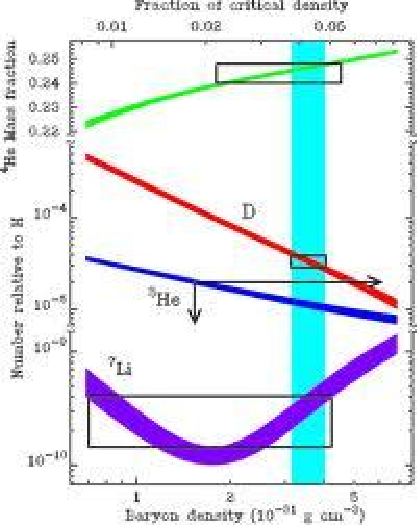
\includegraphics[width=0.5\textwidth]{figure/Abundances.pdf}
  \caption{Abbondanza vs $\rho_B(t_0)$}
  \label{fig:abbondanza}
\end{figure}

\section{Teoria dell'inflazione}
\label{sec:inflazione}

\emph{Queste note sono basate sulle lezioni di Inflazione tenute da Danièle
  Steer (APC Paris) durante l'IDPASC School 2015.}

\subsection{Problemi del modello standard della cosmologia}
\label{sec:problemi-cosmologia}

Il modello dell'Hot Big Bang è perfettamente soddisfacente per tempi \(t\gtrsim
\SI{e-3}{\second}\) dopo la singolarità iniziale, quindi prima della
nucleosintesi del Big Bang.  Questo modello è compatibile con la legge di Hubble
e descrive bene la nucleosintesi, la presenza di una radiazione di fondo a
microonde e la formazione e crescita delle struttura a larga scala.

Tuttavia, il modello è incompleto dal momento che le condizioni iniziali devono
essere fissate a mano.  Inoltre, ci sono alcuni problemi tuttora irrisolti, fra
i quali:
\begin{itemize}
\item l'origine e la natura della materia e dell'energia oscura,
\item il \emph{problema dei monopoli magnetici},
\item il \emph{problema della piattezza},
\item il \emph{problema dell'orizzonte}.
\end{itemize}
La teoria dell'\emph{inflazione}, sviluppata a partire dagli anni '70 del secolo
scorso soprattutto da parte di Guth e Linde, afferma che pochi istanti dopo il
Big Bang c'è stata una breve fase di rapida espansione accelerata dell'Universo,
quindi caratterizzata da \(\ddot{R}>0\).  La fase di inflazione sarebbe iniziata
circa \SI{e-36}{\second} dopo il Big Bang e sarebbe terminata fra circa
\SI{e-34}{\second} e \SI{e-32}{\second} dopo la singolarità iniziale.  Questo
fenomeno, se fosse avvenuto realmente, risolverebbe in un colpo solo tutti gli
ultimi tre problemi elencati.

La teoria dell'inflazione è un'aggiunta al modello standard della cosmologia,
non una nuova teoria alternativa a quella finora illustrata che rimane per il
resto inalterata.  A oggi non sono ancora state trovate evidenze sperimentali
che dimostrino la validità dell'inflazione, anche se ci sono forti motivazioni
teoriche che la fanno apparire ben fondata.

Nei seguenti paragrafi illustreremo i problemi dei monopoli magnetici, della
piattezza e dell'orizzonte, facendo inoltre vedere come la fase di inflazione li
risolverebbe.

\subsection{Problema dei monopoli magnetici}
\label{sec:problema-monopoli}

Secondo alcune teorie della grande unificazione, al termine della fase di
unificazione delle forze (\SI{e-36}{\second} dopo il Big Bang) si sarebbe
formato un gran numero di \emph{monopoli magnetici} (ipotetiche particelle
dotate di singola carica del campo magnetico) dotate di massa elevata.  Secondo
alcune stime~\parencite[143-145]{2002coec.book.....C}, i monopoli magnetici
dovrebbero avere massa \(m_{\textup{M}} \approx \SI{e16}{\giga\electronvolt}\) e
densità numerica attuale, escludendo che ci sia stata una fase di inflazione,
almeno dello stesso ordine di quella dei barioni.  Questo è chiaramente
incompatibile con le osservazioni attuali perché i monopoli magnetici non sono
mai stati trovati ma, soprattutto, la loro elevata massa combinata con la loro
densità numerica significherebbe che la densità di materia oggi dovrebbe essere
\(16\) ordini di grandezza più grande di quella misurata.

La fase di inflazione risolverebbe questo problema perché l'espansione
accelerata si collocherebbe dopo la formazione dei monopoli magnetici ma prima
della creazione della materia ordinaria che costituisce l'Universo che
conosciamo.  Pertanto, la rapida espansione porterebbe a una forte diminuzione
della densità dei soli monopoli magnetici, senza alterare la densità della
materia barionica.  Per fissare le idee, anticipiamo che il fattore di scala fra
l'inizio e la fine della fase di inflazione sarebbe aumentato di circa \num{e26}
volte, quindi la densità di monopoli sarebbe diminuita di un fattore dell'ordine
di \num{e78}.

\subsection{Problema della piattezza}
\label{sec:problema-piattezza}

Richiamiamo l'equazione di Friedmann~\eqref{eq:friedmann} nella forma
\begin{equation}
  \label{eq:friedmann2}
  H^{2}(t) = \left(\frac{\dot{R}(t)}{R(t)}\right)^{2} = \frac{8\pi G}{3}\rho(t)
  - \frac{k}{R^{2}(t)}.
\end{equation}
Con il parametro di densità \(\Omega(t) = \rho(t)/\rho_{\textup{c}}(t)\) si può
riscrivere come
\begin{equation}
  \label{eq:friedmann-densita}
  \Omega(t) - 1 = \frac{k}{R^{2}(t)H^{2}(t)}.
\end{equation}
Secondo gli ultimi dati del telescopio Planck~\parencite{2015arXiv150201589P},
oggi risulta \(\abs{\Omega(t_{0}) - 1} = \num{0.000(5)}\), cioè
\(\abs{\Omega(t_{0}) - 1} < \num{0.005}\).  Questo significa che oggi l'Universo
appare pressoché piatto.  Dall'analisi
dell'equazione~\eqref{eq:friedmann-densita} possiamo dedurre che
\begin{itemize}
\item o la costante \(k\) è nulla e quindi \(\Omega(t) - 1\) è sempre stata
  uguale a \(0\),
\item oppure \(\abs{\Omega(t) - 1}\) si evolve nel tempo come \((R(t)H(t))^{-2}
  = \dot{R}^{-2}(t)\).
\end{itemize}

Prima di procedere, ricordiamo che dall'equazione di
continuità~\eqref{eq:continuita} \(\dot{\rho} + 3H(p + \rho) = 0\) si ricava che
\begin{equation}
  \rho(R) \sim R^{-3(1+w)}
\end{equation}
con \(w = p/\rho\).  Poiché stiamo considerando un Universo approssimativamente
piatto, poniamo per semplicità \(k=0\) nell'equazione~\eqref{eq:friedmann2} e
inserendo il risultato precedente si ha
\begin{equation}
  \begin{split}
    H^{2} = \left(\frac{\dot{R}}{R}\right)^{2} \sim \rho = R^{-3(1+w)} &\implies
    \frac{1}{R} \toder{R}{t} \sim R^{-3(1+w)/2} \\
    &\implies R^{(3w+1)/2}\dd R \sim \dd t.
  \end{split}
\end{equation}
La soluzione di questa equazione differenziale dipende dal valore di \(w\).  Se
\(w\neq -1\) allora si trova che
\begin{equation}
  R(t) \sim t^{2/3(w+1)} = t^{\beta}
\end{equation}
con
\begin{equation}
  \beta = \frac{2}{3(w+1)} =
  \begin{cases}
    2/3 & \text{per la materia (\(w = 0\))}, \\
    1/2 & \text{per la radiazione (\(w = 1/3\))}.
  \end{cases}
\end{equation}
Invece se \(w = -1\) si ha che
\begin{equation}
  R(t) \sim \e^{Ht}.
\end{equation}
Ricapitolando abbiamo determinato
\begin{equation}
  R(t) \sim
  \begin{cases}
    t^{\beta} & \text{se \(w\neq -1\)}, \\
    \e^{Ht}  & \text{se \(w = -1\)}.
  \end{cases}
\end{equation}

\begin{figure}
  \centering
  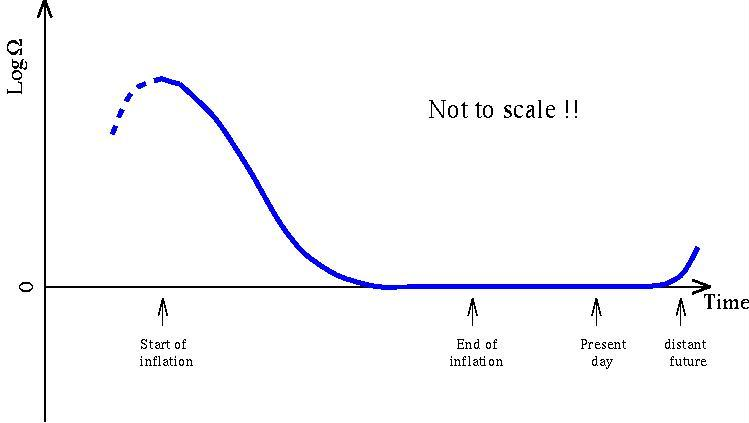
\includegraphics[width=\textwidth]{figure/flatness}
  \caption[Come l'inflazione risolve il problema della piattezza]{La teoria
    dell'inflazione risolve il problema della piattezza introducendo una fase in
    cui \(\abs{\Omega(t) - 1}\), rappresentata sull'asse delle ordinate, tende
    rapidamente verso \(0\), partendo da una condizione iniziale qualsiasi.  Al
    termine della fase di inflazione, \(\abs{\Omega(t) - 1}\) ha ripreso
    lentamente ad aumentare fino a raggiungere il valore attuale.  Immagine
    tratta da \url{https://ned.ipac.caltech.edu/level5/Liddle/Liddle4_1.html}}
  \label{fig:piattezza}
\end{figure}
Ora possiamo calcolare l'evoluzione di \(\abs{\Omega(t) - 1}\) con il tempo.
Supponiamo che l'Universo sia stato dominato solo dalla radiazione e dalla
materia, quindi possiamo assumere che risulti sempre \(\beta < 1\).  In questo
modo vediamo che
\begin{equation}
  \label{eq:omega-t}
  \abs{\Omega(t) - 1} \sim \dot{R}^{-2}(t) \sim \frac{t^{2(1-\beta)}}{\beta^{2}}
\end{equation}
è una funzione crescente col tempo.  Dunque, oggi l'Universo ha una densità
prossima alla densità critica, ma per quanto abbiamo trovato in passato la
densità era ancora più vicina alla densità critica.  Possiamo stimare quanto è
aumentato \(\abs{\Omega(t) - 1}\) fra il tempo di Planck \(t = t_{\textup{Pl}}
\sim \SI{e-43}{\second}\) e oggi (\(t = t_{0} \sim \SI{e17}{\second}\)).  Per
fare questo supponiamo un Universo sempre dominato dalla radiazione, quindi vale
sempre \(\beta = 1/2 \implies \abs{\Omega(t) - 1} \sim t\), da cui
\begin{equation}
  \frac{\abs{\Omega(t_{0}) - 1}}{\abs{\Omega(t_{\textup{Pl}}) - 1}} \sim
  \frac{10^{17}}{10^{-43}} = 10^{60}.
\end{equation}
Inoltre abbiamo visto che oggi si ha \(\abs{\Omega(t_{0}) - 1} \lesssim
10^{-3}\), quindi
\begin{equation}
  \abs{\Omega(t_{\textup{Pl}}) - 1} \lesssim 10^{-63}.
\end{equation}
Con questi approssimativi calcoli abbiamo trovato che subito dopo il Big Bang la
densità dell'Universo doveva differire dalla densità critica al più per una
parte su \(10^{-63}\).  Il modello standard della cosmologia non prevede che
l'Universo dovesse essere all'inizio praticamente piatto o quasi, bisogna
imporlo come condizione iniziale.  Questo non è un vero e proprio problema di
per sé, ma è un difetto nella teoria del modello standard perché comporta
fissare forzatamente la densità iniziale dell'Universo a un valore molto
particolare, quando non ci sono motivi per ritenere che questo valore fosse più
probabile di qualsiasi altro.  Si usa dire che questo è un problema di
\emph{fine-tuning}.

Il problema della piattezza sarebbe risolto se ci fosse stata una fase, nel
passato, in cui \(\abs{\Omega(t) - 1}\) fosse rapidamente sceso verso \(0\).
Questa è proprio la fase di inflazione.  Dall'equazione~\eqref{eq:omega-t} si
vede che questo è possibile se risulta \(\beta > 1\).  In questo caso
\(\abs{\Omega(t) - 1} \to 0\) è un attrattore per l'evoluzione del sistema,
qualunque sia stato il valore iniziale.  L'inflazione risolve dinamicamente il
problema del \emph{fine-tuning}: la densità iniziale dell'Universo aveva
effettivamente un valore qualsiasi, solo successivamente si è evoluta verso la
densità critica, per poi allontanarsi lentamente da essa al termine della fase
di inflazione, come mostrato nella figura~\ref{fig:piattezza}.

Osserviamo che se \(\beta>1\) risulta \(\ddot{R} = \beta(\beta-1)t^{\beta-2}
\implies \ddot{R} > 0\), cioè espansione accelerata dell'Universo, proprio come
prescritto dalla teoria dell'inflazione.  D'altra parte \(\beta = 2/3(w+1)>1\)
equivale a \(-1 < w < -1/3\) e dall'equazione di accelerazione
\(\ddot{R}/R=-4\pi G(\rho+3p)/3\) si ha che si ha espansione accelerata solo se
\(w < -1/3\).

\subsection{Problema dell'orizzonte}
\label{sec:problema-orizzonte}

L'origine di questo problema è la \emph{causalità}: la velocità della luce nel
vuoto fissa un limite superiore alla velocità di propagazione di qualsiasi
segnale.  Le mappe della radiazione cosmica di fondo realizzate dai telescopi
WMAP e Planck hanno mostrato che l'intero cielo a noi oggi visibile ha la stessa
temperatura, a meno di anisotropie dell'ordine di \(10^{-5}\), quindi
trascurabili in prima analisi.  È possibile che tutti i punti di una così vasta
regione dello spazio fossero in connessione causale al momento del
disaccoppiamento, in modo tale da giustificare un processo di termalizzazione
che abbia coinvolto tutto l'Universo visibile?

Definiamo \emph{orizzonte} \(d_{\textup{H}}(t,t_{i})\) come la massima distanza
percorsa da un raggio di luce emesso al tempo \(t_{i}\) e osservato al tempo
\(t\).  Questa quantità determina la distanza massima che ci può essere fra due
punti che sono in connessione causale l'uno con l'altro.  Matematicamente
abbiamo
\begin{equation}
  d_{\textup{H}}(t, t_{i}) = R(t)\int_{t_{i}}^{t} \frac{\dd t'}{R(t')} =
  \frac{R(t)}{1-\beta}(t^{1-\beta} - t_{i}^{1-\beta})
\end{equation}
avendo usato \(R(t)\sim t^{\beta}\).  Vogliamo determinare cosa succede provando
a considerare un segnale partito molto indietro nel tempo, diciamo per \(t_{i}
\to 0\).  Ci sono due possibilità:
\begin{itemize}
\item \(d_{\textup{H}}(t, t_{i})\) converge a un valore finito per \(t_{i} \to
  0\) e in questo caso il segnale emesso non può essere visto più lontano della
  distanza \(d_{\textup{H}}(t, t_{i})\),
\item oppure l'integrale diverge a un valore infinito, quindi è possibile
  ricevere segnali emessi a tempi sufficientemente remoti da qualsiasi sorgente
  comovente.
\end{itemize}
In un Universo sempre dominato solo da radiazione e materia risulta \(\beta<1\)
e quindi
\begin{equation}
  d_{\textup{H}}(t, t_{i}) \xrightarrow[t_{i}\to 0]{} \frac{R(t)
    t^{1-\beta}}{1-\beta} = \frac{\beta}{1-\beta} \frac{1}{H(t)}
\end{equation}
A parte il fattore numerico legato al valore di \(\beta\), la dimensione
dell'orizzonte è essenzialmente data dal raggio di Hubble \(1/H(t)\) e ci
troviamo nella prima delle due situazioni illustrate sopra.  Secondo questo
modello, col passare del tempo aumentano le frazioni dell'Universo che sono in
connessione causale.  Quindi esistono nella radiazione cosmica di fondo delle
regioni che erano disconnesse causalmente.  Ma a questo punto sorge il problema:
come è possibile spiegare l'omogeneità delle condizioni iniziali al momento
dell'ultimo scattering, quando è iniziata la radiazione cosmica di fondo?
Ancora una volta l'inflazione risolve il problema introducendo una fase con
\(\beta>1\), che abbiamo visto implicare espansione accelerata \(\ddot{R}>0\).
In questo caso si ha
\begin{equation}
  d_{\textup{H}}(t, t_{i}) \xrightarrow[t_{i}\to 0]{} \infty
\end{equation}
e sarebbe quindi stato possibile, per tutti i punti della radiazione che
osserviamo oggi, essere in connessione causale l'uno con l'altro.

\begin{figure}
  \centering
  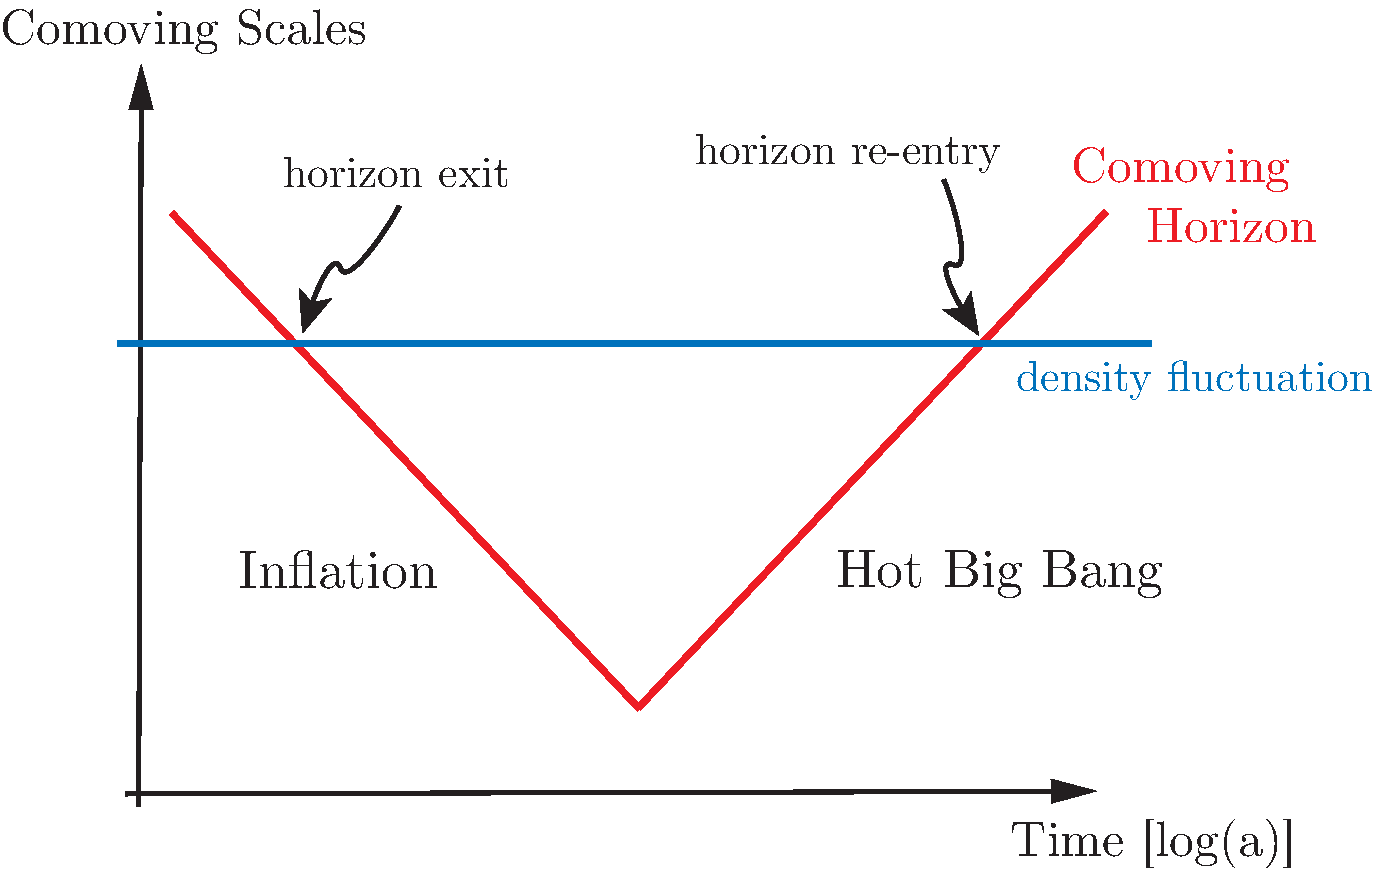
\includegraphics[width=0.55\textwidth]{figure/scales}\hfill
  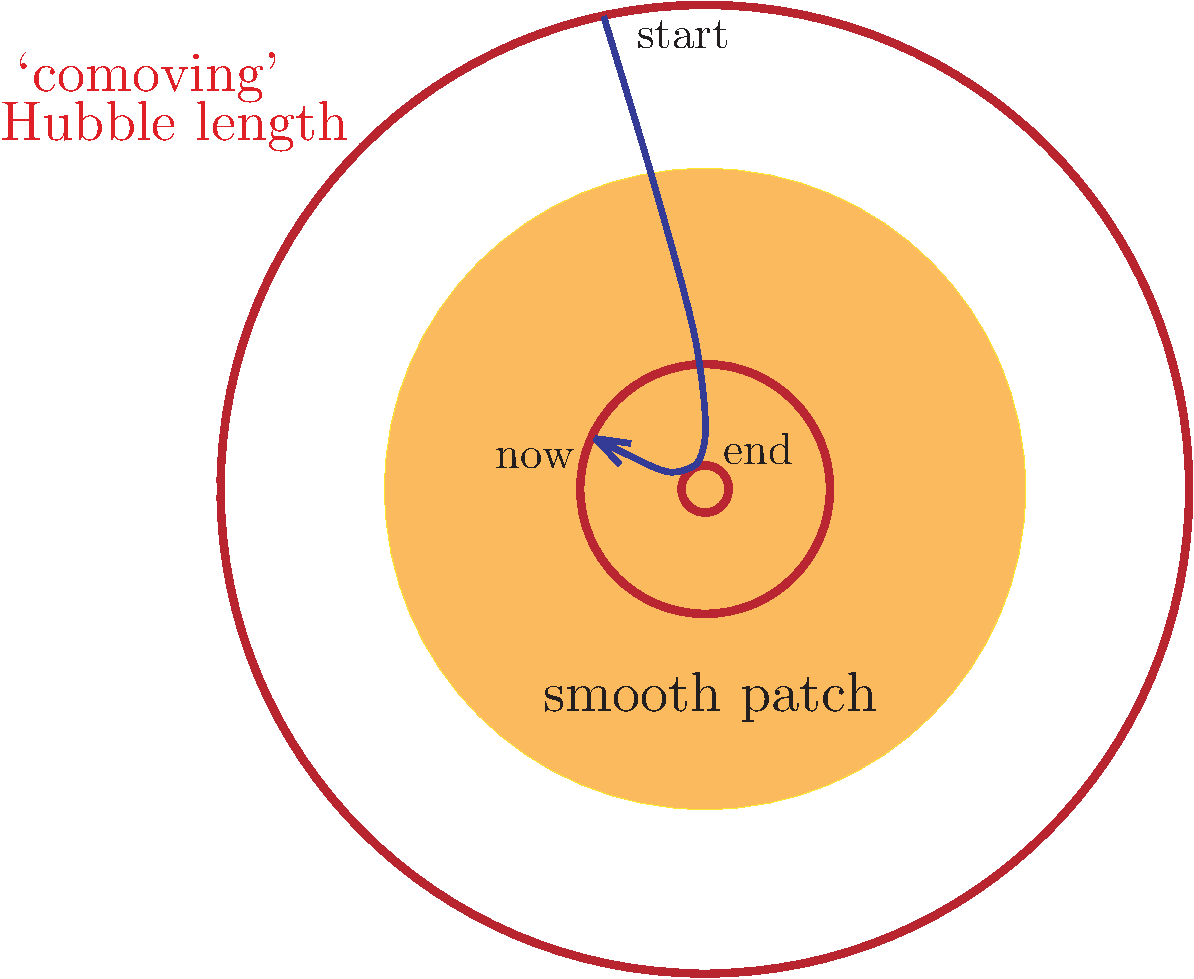
\includegraphics[width=0.4\textwidth]{figure/horizon}
  \caption[Come l'inflazione risolve il problema
  dell'orizzonte]{\emph{Sinistra}: andamento schematico del raggio comovente di
    Hubble \((RH)^{-1}\) con il tempo.  Durante l'inflazione è diminuito, per
    poi crescere nelle epoche della radiazione e della materia, previste dal
    modello dell'Hot Big Bang.  I punti che si trovano a una distanza pari al
    raggio comovente di Hubble attuale oggi sono in contatto causale, ma secondo
    quest'ultimo modello non possono mai esserlo stato nel passato.  Invece, se
    c'è stata una fase di inflazione le distanze dell'ordine di \((RH)^{-1}\)
    attuale sono state al di sotto dell'orizzonte in tempi sufficientemente
    remoti.  \emph{Destra}: evoluzione del raggio comovente di Hubble.  La sfera
    comovente di Hubble si è ristretta durante l'inflazione e allargata in
    seguito.  Figure tratte da~\cite[27]{2009arXiv0907.5424B}}
  \label{fig:orizzonte}
\end{figure}
Proviamo a illustrare un altro argomento che presenta il problema
dell'orizzonte.  Già nel problema della piattezza abbiamo incontrato
l'importante quantità
\begin{equation}
  \frac{1}{R(t)H(t)}
\end{equation}
chiamata \emph{raggio} o \emph{parametro di Hubble comovente}.  Il nome deriva
dal fatto che \(c/H(t) = 1/H(t)\) è il \emph{raggio di Hubble}, che indica la
tipica lunghezza di scala alla quale un processo fisico nell'Universo opera
coerentemente.  Dividendo per il fattore di scala si ottiene la corrispondente
grandezza comovente, che tiene conto della variazione di \(R(t)\).  Vediamo come
si evolve il parametro di Hubble comovente con il tempo.  Per parametrizzare il
tempo usiamo il fattore di scala, che sappiamo avere andamento \(R(t)\sim
t^{\beta}\), se \(w\neq -1\).  Nel caso dell'Universo dominato dalla radiazione
\(\beta = 1/2\), quindi
\begin{equation}
  \ln \frac{1}{RH} = \ln \frac{1}{\dot{R}} \sim \ln t^{1/2} \sim \ln R.
\end{equation}
Invece, nella fase dell'Universo dominato dalla materia abbiamo \(\beta = 2/3\),
da cui
\begin{equation}
  \ln \frac{1}{RH} = \ln \frac{1}{\dot{R}} \sim \ln t^{1/3} \sim \ln R^{1/2} =
  \frac{1}{2}\ln R.
\end{equation}
Quindi in ogni caso \(\ln (RH)^{-1}\) è una funzione crescente di \(\ln R\).  Ma
questo significa che regioni che oggi vediamo essere in contatto causale in
passato non potevano esserlo, dato che il raggio comovente di Hubble in passato
era molto più piccolo, quindi non c'è potuto essere un processo di
termalizzazione su una scala così grande.  Il problema si risolverebbe se in
passato, prima dell'inizio dell'epoca dominata dalla radiazione, c'è stata una
fase in cui \((RH)^{-1}\) è diminuito con il tempo, e quindi con \(R\).
Condizione necessaria affinché \((RH)^{-1}\) diminuisca con il tempo è che la
sua derivata temporale sia negativa, cioè
\begin{equation}
  0 > \toder{}{t} \frac{1}{RH} = \frac{1}{\dot{R}} =
  -\frac{\ddot{R}}{(\dot{R})^{2}} \iff \ddot{R}>0.
\end{equation}
Abbiamo di nuovo trovato che una fase inflazionaria di espansione accelerata
risolverebbe il problema dell'orizzonte: l'Universo prima dell'inflazione aveva
un raggio comovente di Hubble più grande di quello attuale, durante l'inflazione
il raggio è diminuito rapidamente, per poi ricominciare a crescere durante le
epoche della radiazione e della materia.  Le scale che noi oggi vediamo entrare
in connessione casuale lo erano già state in passato, prima dell'era della
radiazione, ed è in quel periodo che erano in corso i processi di
omogeneizzazione delle condizioni iniziali che hanno poi permesso alla
radiazione cosmica di fondo di avere una temperatura uniforme fra regioni che
credevamo non aver mai potuto comunicare fra di loro.  Per concretezza, durante
l'inflazione si assume che \(H\) sia rimasto costante, quindi
\begin{equation}
  \ln \frac{1}{RH} = \ln \frac{1}{R \cdot \text{costante}} \sim \ln \frac{1}{R}
  = - \ln R.
\end{equation}
Nella figura~\ref{fig:orizzonte} è rappresentato schematicamente l'andamento del
raggio comovente di Hubble secondo la teoria dell'inflazione.

\subsection{Quanta inflazione?}
\label{sec:quanta-inflazione}

Vogliamo determinare quanta inflazione c'è stata, cioè di quanto è aumentato il
fattore di scala durante la fase inflazionaria.  Calcoleremo questa quantità
prendendo spunto dal problema della piattezza.

Nella teoria dell'inflazione si quantifica l'espansione con il logaritmo del
rapporto fra il fattore di scala alla fine dell'inflazione (\(t_{f}\)) e
all'inizio (\(t_{i}\))
\begin{equation}
  N_{*} = \ln \frac{R(t_{f})}{R(t_{i})}.
\end{equation}
Questa quantità è chiamata \emph{numero di \(\e\)-foldings}, perché indica
quante \(\e = 2.718\dots\) volte si è espanso l'Universo in quella fase.

Assumiamo, senza perdita di generalità, che \(\abs{\Omega(t) - 1}\) all'inizio
dell'inflazione fosse dell'ordine dell'unità,\footnote{L'importante è che sia
  sostanzialmente diversa da \(0\).} quindi \(\abs{\Omega(t_{i}) - 1} \sim 1\).
Oggi sappiamo che risulta al più \(\abs{\Omega(t_{0}) - 1} \sim 0.001\), per
determinare \(\abs{\Omega(t_{f}) - 1}\) sfruttiamo \(\abs{\Omega(t) -1} \sim
t^{2(1-\beta)}\) e andiamo a ritroso nel tempo.  Ricordiamo che
\begin{itemize}
\item l'era della radiazione (\(\beta = 1/2\)) è iniziata al termine
  dell'inflazione (\(t \sim \SI{e-34}{\second}\)) ed è finita a \(t =
  \SI{4.7e4}{y} = \SI{1.5e12}{\second}\);
\item l'era della materia (\(\beta = 2/3\)) è iniziata al termine dell'era della
  radiazione ed è continuata quasi fino ai giorni nostri\footnote{Trascuriamo
    l'era dell'energia oscura, ininfluente ai fini di questi calcoli.} \(t =
  \SI{13.8e9}{y} = \SI{4.4e17}{\second}\).
\end{itemize}
Quindi risulta
\begin{equation}
  \abs{\Omega(t_{f}) - 1} = \abs{\Omega(t_{f}) - 1}
  \left(\frac{\num{4.4e17}}{\num{1.5e12}}\right)^{2(2/3-1)}
  \left(\frac{\num{1.5e12}}{\num{e-34}}\right)^{2(1/2-1)} = \num{1.5e-53}.
\end{equation}
Durante l'inflazione si assume \(H(t) = \text{costante}\), quindi in questa fase
\(\abs{\Omega(t_{f}) - 1} \sim R^{-2}\) e
\begin{equation}
  \frac{R(t_{f})}{R(t_{i})} = \sqrt{\frac{\abs{\Omega(t_{i}) -
        1}}{\abs{\Omega(t_{f}) - 1}}} = \num{2.6e26},
\end{equation}
da cui troviamo infine
\begin{equation}
  N_{*} = \ln \frac{R(t_{f})}{R(t_{i})} \approx 61.
\end{equation}
Dunque, usando come punto di partenza il problema dell'orizzonte, abbiamo
trovato che durante la breve fase di inflazione il fattore di scale è aumentato
di un fattore dell'ordine di \(10^{26}\), corrisponde a un numero di e-foldings
pari a circa \(60\).

\subsection{Inflazione vs energia oscura}
\label{sec:inflazione-energia-oscura}

Sia la fase di inflazione sia l'era dominata dall'energia oscura nella quale ci
troviamo oggi sono caratterizzate dall'espansione accelerata dell'Universo,
\(\ddot{R} > 0\), ma ci sono due differenze sostanziali fra queste due
situazioni
\begin{itemize}
\item le energie in gioco sono completamente differenti, infatti si calcola che
  il potenziale associato all'inflazione è dell'ordine di (\(M_{\textup{Pl}} =
  1/\sqrt{8\pi G}\) è la massa di Planck)
  \begin{equation}
    V_{\textup{inflazione}} \sim (M_{\textup{Pl}})^{4}
  \end{equation}
  mentre per l'energia oscura si trova
  \begin{equation}
    V_{\textup{energia oscura}} \sim (10^{-30}M_{\textup{Pl}})^{4}.
  \end{equation}
  Questo giustifica anche il fatto che il fattore di scala durante l'inflazione
  è aumentato in maniera molto più rapida rispetto all'aumento in corso oggi;
\item la fase di inflazione si è dovuta arrestare a un certo punto della storia
  dell'Universo, per dare spazio alle ere di dominio della radiazione e della
  materia, mentre non conosciamo ancora il destino dell'espansione attuale
  guidata dall'energia oscura, che in base alle nostre conoscenze potrebbe anche
  durare per sempre.
\end{itemize}

\subsection{Regime di slow-roll e potenziale di inflazione}
\label{sec:slow-roll}

La costante cosmologica è un esempio di modello per descrivere un Universo in
espansione accelerata, ma abbiamo ricordato che l'inflazione deve avere
necessariamente avuto una fine.  Affinché questo sia avvenuto, c'è bisogno di
introdurre una dipendenza dal tempo nel modello dell'inflazione e si fa questo
introduce un campo scalare inflatonico \(\phi\) che guida l'evoluzione
dell'Universo in questa fase, con un potenziale associato \(V(\phi)\) che evolve
nel tempo.  In questo paragrafo vedremo sotto quali condizioni si verifica la
fase di inflazione.

Per descrivere l'inflazione si aggiunge all'azione del campo gravitazionale
l'azione associata al campo inflatonico \(\phi\) data da
\begin{equation}
  S_{\phi} = \int\dd^{4}x
  \sqrt{-g}\left(-\frac{1}{2}(\partial_{\mu}\phi)(\partial^{\mu}\phi) -
    V(\phi)\right)
\end{equation}
da cui si ricava il tensore di energia-impulso
\begin{equation}
  T_{\mu\nu} = \frac{2}{\sqrt{-g}} \frac{\delta S_{\phi}}{\delta g_{\mu\nu}}
  = \partial_{\mu}\phi \partial_{\nu}\phi -
  g_{\mu\nu}\left(\frac{1}{2}\partial_{\sigma}\phi \partial^{\sigma}\phi -
    V\right)
\end{equation}
e l'equazione del moto
\begin{equation}
  \nabla_{\mu}\nabla^{\mu}\phi = \toder{V}{\phi}.
\end{equation}
Inoltre si possono calcolare la pressione e la densità del campo inflatonico
\begin{align}
  \rho &= -\tensor{T}{^{0}_{0}} = \frac{1}{2}\dot{\phi}^{2} + V, \\
  p &= \frac{1}{2}\dot{\phi}^{2} - V.
\end{align}
L'equazione del moto si può riscrivere come
\begin{equation}
  \ddot{\phi} + 3H\dot{\phi} + V' = 0,
\end{equation}
in cui \(V' = \ltoder{V}{\phi}\).  L'equazione di stato stato del campo
inflatonico è
\begin{equation}
  w = \frac{p}{\rho} = \frac{\dot{\phi}^{2}/2 - V}{\dot{\phi}^{2}/2 + V}.
\end{equation}
Risulta \(-1<w<1\), con \(-1\) corrispondente al caso limite \(\dot{\phi}^{2}/2
\ll V\) e \(1\) al caso \(\dot{\phi}^{2}/2 \gg V\).  L'inflazione richiede che
ci sia espansione accelerata e come abbiamo già visto questo corrisponde alla
condizione \(w < -1/3\), quindi l'energia cinetica del campo è molto più piccola
del potenziale.  Questo porta alla definizione del \emph{regime di slow-roll},
durante il quale, secondo le moderne teorie dell'inflazione, è avvenuta
l'espansione accelerata primordiale.  Lo slow-roll è caratterizzato da due
condizioni
\begin{itemize}
\item energia cinetica del campo inflatonico molto più piccola del suo
  potenziale, \(\dot{\phi}^{2}/2 \ll V\);
\item accelerazione del campo trascurabile nell'equazione del moto,
  \(\abs{\ddot{\phi}}\ll \abs{3H\dot{\phi}}\), \(\abs{V'}\).
\end{itemize}
Dalla prima condizione abbiamo che l'equazione di Friedmann si può scrivere come
\begin{equation}
  H^{2} = \frac{8\pi G}{3}\rho \approx \frac{8\pi G}{3}V
\end{equation}
e dalla seconda condizione l'equazione del moto diventa
\begin{equation}
  3H\dot{\phi} + V' = 0.
\end{equation}
Inoltre risulta \(w \approx -1\), quindi durante l'inflazione il fattore di
scala va come \(R(t)\sim \e^{Ht}\).

Nelle teorie d'inflazione si introducono due parametri
\begin{align}
  \epsilon_{V} &\equiv
  \frac{M_{\textup{Pl}}^{2}}{2}\left(\frac{V'}{V}\right)^{2}, \\
  \eta_{V} &\equiv M_{\textup{Pl}}^{2}\frac{V''}{V}.
\end{align}
Usando entrambe le condizioni che determinano il regime di slow-roll si vede che
affinché si abbia l'inflazione deve risultare
\begin{align}
  \epsilon_{V} &\ll 1, \\
  \abs{\eta_{V}} &\ll 1.
\end{align}
La fase di inflazione termina quando le condizioni di slow-roll non sono più
soddisfatte.  In particolare, calcolando \(\dot{H} = \ddot{R}/R - H^{2}\) si può
ricavare che \(\ddot{R}/R = H^{2}(1 - \epsilon_{V})\), quindi l'inflazione ha
avuto fine quando si è raggiunta la condizione
\begin{equation}
  \ddot{R} = 0 \implies \epsilon_{V} = 1.
\end{equation}

Esistono diversi modelli di inflazione: tutti prevedono una breve fase di rapida
espansione accelerata, ma cambiano i parametri del sistema, come il numero di
e-foldings, e l'espressione del potenziale inflatonico.  Riportiamo che in base
alle ultime analisi fatte dalla collaborazione di
Planck~\parencite{2015arXiv150202114P} il potenziale che risulta favorito è il
\emph{potenziale di Starobinsky}
\begin{equation}
  V(\phi) \propto (1 - \e^{\sqrt{2/3}\phi/M_{\textup{Pl}}})^{2}
\end{equation}
e con \(N_{*} = 60\).  Questo modello è anche chiamato \emph{inflazione
  \(R^{2}\)} perché si modifica l'azione del campo gravitazionale aggiungendo un
termine quadratico nella curvatura scalare \(S \sim \int\dd^{4}x\sqrt{-g}(R +
R^{2})\).

%%% Local Variables:
%%% mode: latex
%%% TeX-master: "../cosmo"
%%% fill-column: 80
%%% End:


\appendix{}
\cleardoublepage
\chapter{Teorema di Gauss nello spazio di Minkowski}
\label{cha:teorema-gauss}

Il \index{teorema!di Gauss}teorema di Gauss in $\M$ mette in relazione
l'integrale di volume (spaziotemporale) della quadridivergenza di un
quadrivettore $V^{\alpha}(x)$ con un integrale di ipersuperficie di
$V^{\alpha}(x)$
\begin{equation}
  \int\limits_{\Omega} \partial_{\alpha}V^{\alpha}(x) \dd^{4} x =
  \int\limits_{\partial\Omega} V^{\alpha}(x) \dd\Sigma_{\alpha},
\end{equation}
in cui $\partial\Omega$ è l'ipersuperficie di contorno del volume
quadrimensionale $\Omega$. Il quadrivettore $\dd\Sigma_{\alpha}$ è l'elemento di
ipersuperficie
\begin{equation}
  \dd\Sigma_{\alpha} = (\dd x^{1}\dd x^{2}\dd x^{3}, \dd x^{0}\dd x^{2}\dd
  x^{3}, \dd x^{0}\dd x^{1}\dd x^{3}, \dd x^{0}\dd x^{1}\dd x^{2})
\end{equation}
che ha come direzione la normale all'ipersuperficie e come modulo la sua area
$\dd\Sigma$.

\begin{figure}
  \centering
  \tdplotsetmaincoords{70}{100}
  \begin{tikzpicture}[tdplot_main_coords,font=\footnotesize,scale=5,
    piano/.style={gray!20!white,opacity=0.85}]
    \node[shape=coordinate] (O1) at (0,0,0) {};
    \draw[->] (O1) -- ++(1,0,0) node[anchor=north east] {$x$}; % asse x
    \draw[->] (O1) -- ++(0,1,0) node[anchor=north west] {$y$}; % asse y
    \draw[->] (O1) -- ++(0,0,1) node[anchor=south] {$t$}; % asse temporale
    \filldraw[piano] (0,0,0.1) node[black,left] {$t_{1}$} -- ++(0,1,0) --
    ++(1,0,0) node[black,above left] {$\Sigma_{1}$} -- ++(0,-1,0) -- ++(-1,0,0);
    \filldraw[piano] (0,0,0.9) node[black,left] {$t_{2}$} -- ++(0,1,0) --
    ++(1,0,0) node[black,above left] {$\Sigma_{2}$} -- ++(0,-1,0) -- ++(-1,0,0);
    \draw[->] (0.5,0.5,0.1) -- ++(0,0,0.3) node[above] {$\versor{n}_{1}$};
    \draw[->] (0.5,0.5,0.9) -- ++(0,0,0.3) node[above] {$\versor{n}_{2}$};
    \node at (0.3,0.3,0.5) {$\Omega$};
  \end{tikzpicture}
  \caption[Volume quadrimensionale delimitato da iperpiani a tempo
  costante]{Volume quadrimensionale $\Omega$ delimitato dagli iperpiani a tempo
    $t$ costante $\Sigma_{1}$ e $\Sigma_{2}$.  Sono riportate solo due
    dimensioni spaziali, $x$ e $y$.  Gli iperpiani $\Sigma_{1}$ e $\Sigma_{2}$
    si estendono verso l'infinito spaziale e sono chiusi dall'iperpiano
    $\Sigma_{\infty}$, non riportato nella figura}
  \label{fig:teorema-gauss}
\end{figure}
Questo teorema ha un'utile applicazione per quanto riguarda i quadrivettori
$V^{\alpha}(x)$ con quadridivergenza nulla
\begin{equation}
  \partial_{\alpha}V^{\alpha}(x) = 0.
\end{equation}
Con riferimento alla figura~\ref{fig:teorema-gauss}, integriamo
$\partial_{\alpha}V^{\alpha}(x)$ sul volume $\Omega$ delimitato da due
ipersuperfici a tempo costante $\Sigma_{1}$ e $\Sigma_{2}$ (cioè parametrizzate
rispettivamente dalle equazioni $t = t_{1}$ e $t = t_{2}$, con $t_{1}$ e $t_{2}$
fissati) e da un'ipersuperficie $\Sigma_{\infty}$ posta all'infinito spaziale.
Per il teorema di Gauss risulta
\begin{equation}
  0 = \int\limits_{\Omega} \partial_{\alpha}V^{\alpha}(x) \dd^{4}x =
  \int\limits_{\Sigma_{2}} V^{\alpha}(x) \dd\Sigma_{\alpha} -
  \int\limits_{\Sigma_{1}} V^{\alpha}(x) \dd\Sigma_{\alpha} +
  \int\limits_{\Sigma_{\infty}} V^{\alpha}(x) \dd\Sigma_{\alpha}.
\end{equation}
Il segno meno davanti all'integrale su $\Sigma_{1}$ è dovuto al fatto che
abbiamo orientato le normali $\versor{n}_{1}$ e $\versor{n}_{2}$ degli
iperpiani, rispettivamente, $\Sigma_{1}$ e $\Sigma_{2}$ nel verso crescente del
tempo.  Se $V^{\alpha}(x)$ tende abbastanza rapidamente a $0$ all'infinito
spaziale, il terzo integrale nell'equazione precedente è nullo e quindi
\begin{equation}
  \int\limits_{\Sigma_{2}} V^{\alpha}(x) \dd\Sigma_{\alpha} =
  \int\limits_{\Sigma_{1}} V^{\alpha}(x) \dd\Sigma_{\alpha}.
\end{equation}
Per l'arbitrarietà della scelta delle ipersuperfici $\Sigma_{1}$ e $\Sigma_{2}$,
ciascuna con la coordinata temporale fissata, dobbiamo concludere che
l'integrale
\begin{equation}
  I(\Sigma) = \int\limits_{\Sigma} V^{\alpha}(x) \dd\Sigma_{\alpha}
\end{equation}
non dipende dall'ipersuperficie $\Sigma$, cioè è una costante rispetto al tempo.
In particolare, se scegliamo un sistema di riferimento nel quale
$\dd\Sigma_{\alpha} = (\dd^{3} \bm{x}, 0, 0, 0)$ allora abbiamo mostrato che
\begin{equation}
  \partial_{\alpha}V^{\alpha}(x) = 0 \implies \int V^{0}(x) \dd^{3} \bm{x} =
  \text{costante in $t$}
\end{equation}
se l'integrale è esteso a una regione spaziale sufficientemente grande in modo
che $V^{\alpha}(x)$ si annulla sul suo bordo.\index{teorema!di Gauss}

In maniera analoga si può far vedere che se per un tensore
$\tensor{T}{^{\alpha\beta}}$ si ha
\begin{equation}
  \partial_{\beta}T^{\alpha\beta} = 0,
\end{equation}
allora il quadrivettore
\begin{equation}
  Q^{\alpha}(\Sigma) = \int\limits_{\Sigma} \tensor{T}{^{\alpha\beta}}\dd
  \Sigma_{\beta},
\end{equation}
in cui $\Sigma$ è una ipersuperficie a tempo costante, non dipende dalla
superficie $\Sigma$ su cui si calcola l'integrale, cioè è indipendente dal
tempo, se l'integrale è esteso a tutto lo spazio tridimensionale.  In
particolare, scelto un sistema di riferimento nel quale
$\dd\Sigma_{\beta} = (\dd^{3} \bm{x}, 0, 0, 0)$, risulta
\begin{equation}
  \partial_{\beta}T^{\alpha\beta} = 0 \implies Q^{\alpha} = \int\limits_{\Sigma}
  T^{\alpha0} \dd^{3} \bm{x} = \text{costante in $t$}.
\end{equation}

Più in generale il \index{teorema!di Gauss}teorema di Gauss per un tensore
$T^{\alpha_{1}\alpha_{2}\dots\alpha_{k}}(x)$ di rango $k$ è
\begin{equation}
  \int\limits_{\Omega} \partial_{\alpha_{1}}
  T^{\alpha_{1}\alpha_{2}\dots\alpha_{k}}(x) \dd^{4} x = \int
  T^{\alpha_{1}\alpha_{2}\dots\alpha_{k}}(x) \dd\Sigma_{\alpha_{1}}.
\end{equation}
Se risulta
\begin{equation}
  \partial_{\alpha_{1}} T^{\alpha_{1}\alpha_{2}\dots\alpha_{k}}(x) = 0
\end{equation}
allora l'integrale su un'ipersuperficie $\Sigma$ a tempo fissato
\begin{equation}
  Q^{\alpha_{2}\dots\alpha_{k}}(\Sigma) = \int\limits_{\Sigma}
  T^{\alpha_{1}\alpha_{2}\dots\alpha_{k}}(x) \dd\Sigma_{\alpha_{1}}
\end{equation}
non dipende da $\Sigma$, quindi è costante rispetto al tempo, ed è un tensore di
rango $k-1$.

%%% Local Variables:
%%% mode: latex
%%% TeX-master: "../gravitazione"
%%% fill-column: 80
%%% End:

% TODO: scrivere.  Vedi Weinberg, paragrafo 2.9, pagina 46.  Non l'abbiamo fatto
% a lezione, però lo spin serve per la precessione di De Sitter e mi sembra che
% il Weinberg spieghi abbastanza bene la questione.
\chapter{\completare{Spin}}
\label{cha:spin}


%%% Local Variables: 
%%% mode: latex
%%% TeX-master: "../gravitazione"
%%% End: 

\cleardoublepage
\chapter{Dimostrazioni di alcune relazioni}
\label{cha:dimostrazioni}

\section{Dimostrazione della
  relazione~\texorpdfstring{\eqref{eq:correzione-metrica-controvariante}}
  {(2.32)}}
\label{sec:dimostr-correz-metrica-controvariante}

Nel caso di campo gravitazionale debole, la correzione al tensore metrico
covariante al primo ordine negli infinitesimi è
\begin{equation}
  \label{eq:correzione-metrica-covariante}
  g_{\mu\nu} = \eta_{\mu\nu} + h_{\mu\nu},
\end{equation}
con $h_{\mu\nu} \ll 1$.  Anche $g^{\mu\nu}$ dovrà differire di poco dal tensore
di Minkowski controvariante
\begin{equation}
    \label{eq:correzione-metrica-controvariante2}
  g^{\mu\nu} = \eta^{\mu\nu} + c^{\mu\nu}
\end{equation}
ma le correzioni $c^{\mu\nu}$ alle componenti del tensore metrico controvariante
non sono semplicemente
$c^{\mu\nu} = h^{\mu\nu} = \eta^{\mu\lambda}\eta^{\nu\sigma} h_{\lambda\sigma}$
perché $g^{\mu\nu}$ e $g_{\mu\nu}$ sono legati dalla relazione
\begin{equation}
  g_{\mu\nu}g^{\nu\lambda} = \tensor{\delta}{_{\mu}^{\lambda}}.
\end{equation}
Infatti sostituendo le espressioni~\eqref{eq:correzione-metrica-covariante} e
\eqref{eq:correzione-metrica-controvariante2} dei tensori metrici nell'equazione
precedente abbiamo
\begin{equation}
  \tensor{\delta}{_{\mu}^{\lambda}} = (\eta_{\mu\nu} +
  h_{\mu\nu})(\eta^{\nu\lambda} + c^{\nu\lambda}) =
  \tensor{\delta}{_{\mu}^{\lambda}} + \tensor{c}{_{\mu}^{\lambda}} +
  \tensor{h}{_{\mu}^{\lambda}} + h_{\mu\nu}c^{\nu\lambda},
\end{equation}
quindi deve risultare
\begin{equation}
  0 = \tensor{c}{_{\mu}^{\lambda}} + \tensor{h}{_{\mu}^{\lambda}} +
  h_{\mu\nu}c^{\nu\lambda} \implies \tensor{c}{_{\mu}^{\lambda}} =
  -\tensor{h}{_{\mu}^{\lambda}} - h_{\mu\nu}c^{\nu\lambda}.
\end{equation}
Innalzando in ambo i membri l'indice libero $\mu$ ricaviamo
\begin{equation}
  c^{\mu\lambda} = -h^{\mu\lambda} - \tensor{h}{^{\mu}_{\nu}}c^{\nu\lambda} =
  -h^{\mu\lambda} -\tensor{h}{^{\mu}_{\nu}}(-h^{\nu\lambda} -
  \tensor{h}{^{\nu}_{\rho}} c^{\rho\lambda}) = -h^{\mu\lambda} +
  \tensor{h}{^{\mu}_{\nu}}h^{\nu\lambda} + \mathcal{O}(h^{3}).
\end{equation}
Quindi trascurando termini infinitesimi superiori al terzo ordine, il tensore
metrico controvariante nell'approssimazione di campo debole è dato da
\begin{equation}
  g^{\mu\nu} = \eta^{\mu\nu} + c^{\mu\nu} \approx \eta^{\mu\nu} - h^{\mu\lambda}
  + \tensor{h}{^{\mu}_{\nu}}h^{\nu\lambda}.
\end{equation}
Fermandosi al primo ordine della perturbazione si ha
$g^{\mu\nu} \approx \eta^{\mu\nu} - h^{\mu\nu}$.

\section{Dimostrazione delle
  relazioni~\texorpdfstring{\eqref{eq:g_mu_rho-determinante}}{(3.51)}}
\label{sec:dimostr-determinante}

Sia $A$ una matrice quadrata reale di ordine $n$
\begin{equation}
  A =
  \begin{pmatrix}
    a_{11} & a_{12} & \cdots & a_{1n} \\
    a_{21} & a_{22} & \cdots & a_{2n} \\
    \vdots & \vdots & \ddots & \vdots \\
    a_{n1} & a_{n2} & \cdots & a_{nn}
  \end{pmatrix},
\end{equation}
il suo determinante $D$ si può calcolare, avendo fissato una riga $i$, con lo
\emph{sviluppo di Laplace}
\begin{equation}
  D = \det A = \sum_{j=1}^{n} a_{ij}A_{ij}
\end{equation}
in cui $A_{ij}$ è il \emph{complemento algebrico} dell'elemento $a_{ij}$, cioè
il determinante della matrice che si ottiene da $A$ sopprimendo l'$i$-esima riga
e la $j$-esima colonna moltiplicato per $+1$ se $i+j$ è pari, per $-1$ se $i+j$
è dispari.  Lo sviluppo di Laplace può anche essere svolto fissando la colonna
$j$ e sommando sull'indice di riga $i$.  Dunque, la derivata di $D$ fatta
rispetto all'elemento $a_{ij}$ è il suo coefficiente nello sviluppo di Laplace,
cioè il complemento algebrico corrispondente
\begin{equation}
  \label{eq:deriv-determinante}
  \parder{D}{a_{ij}} = A_{ij}.
\end{equation}

La matrice $B = A^{-1}$ inversa di $A$ con determinante non nullo è quella
matrice di ordine $n$ tale che
\begin{equation}
  A B = B A = I_{n},
\end{equation}
dove $I_{n} = (\delta_{ij})_{i,j=1}^{n}$ è la matrice identità di ordine
$n$. Per la regola di Cramer gli elementi $b_{ij}$ della matrice inversa sono
dati dal rapporto $A_{ji}/D$, cioè la matrice $B$ può essere così scritta
\begin{equation}
  B = A^{-1} =
  \begin{pmatrix}
    b_{11} & b_{12} & \cdots & b_{1n} \\
    b_{21} & b_{22} & \cdots & b_{2n} \\
    \vdots & \vdots & \ddots & \vdots \\
    b_{n1} & b_{n2} & \cdots & b_{nn}
  \end{pmatrix} =
  \begin{pmatrix}
    \dfrac{A_{11}}{D} & \dfrac{A_{21}}{D} & \cdots & \dfrac{A_{n1}}{D} \\[2.0ex]
    \dfrac{A_{11}}{D} & \dfrac{A_{22}}{D} & \cdots & \dfrac{A_{n2}}{D} \\[2.0ex]
    \vdots            & \vdots            & \ddots & \vdots            \\[2.0ex]
    \dfrac{A_{1n}}{D} & \dfrac{A_{2n}}{D} & \cdots & \dfrac{A_{nn}}{D}
  \end{pmatrix}.
\end{equation}
Per la regola di Binet risulta $\det B = 1/\det A = 1/D$.  Inoltre, se la
matrice $A$ è diagonale, si ricava subito che anche $B$ è diagonale con elementi
$b_{ii}=1/a_{ii}$.

Il tensore metrico covariante $g_{\mu\nu}$ è un insieme di $4^{2}$ quantità
reali che possono essere raccolte in una matrice $4 \times 4$
\begin{equation}
  g_{\mu\nu} =
  \begin{pmatrix}
    g_{00} & g_{01} & g_{02} & g_{03} \\
    g_{10} & g_{11} & g_{12} & g_{13} \\
    g_{20} & g_{21} & g_{22} & g_{23} \\
    g_{30} & g_{31} & g_{32} & g_{33}
  \end{pmatrix}.
\end{equation}
Dall'equazione~\eqref{eq:deriv-determinante} abbiamo che la derivata di
$g = -\det(g_{\mu\nu})$ rispetto all'elemento $g_{\mu\nu}$ è
\begin{equation}
  \parder{g}{g_{\mu\nu}} = -\Delta_{\mu\nu},
\end{equation}
in cui $\Delta_{\mu\nu}$ è il complemento algebrico dell'elemento $g_{\mu\nu}$.
Il tensore metrico controvariante $g^{\mu\nu}$ è la matrice inversa di
$g_{\mu\nu}$, quindi, sfruttando la simmetria del tensore metrico, abbiamo
\begin{equation}
  g^{\mu\nu} = g^{\nu\mu} = \frac{\Delta_{\mu\nu}}{-g} =
  \frac{1}{g} \parder{g}{g_{\mu\nu}}.
\end{equation}
Applicando lo stesso ragionamento a $g^{\mu\nu}$ troviamo
($G = -\det(g^{\mu\nu}) = 1/\det(g_{\mu\nu}) = 1/g$)
\begin{equation}
  g_{\mu\nu} = \frac{1}{G} \parder{G}{g^{\mu\nu}} =
  \frac{1}{G} \parder{G}{g} \parder{g}{g^{\mu\nu}} = g \bigg(- \frac{1}{g^{2}}
  \bigg) \parder{g}{g^{\mu\nu}} = - \frac{1}{g} \parder{g}{g^{\mu\nu}}.
\end{equation}

\section{Dimostrazione della
  relazione~\texorpdfstring{\eqref{eq:derivate-miste-vettore}}{(4.17)}}
\label{sec:dimostr-derivate-miste-vettore}

Per calcolare $V_{\mu;\nu;\kappa} - V_{\mu;\kappa;\nu}$ ricordiamo che la
derivata covariante
$V_{\mu;\nu} = V_{\mu,\nu} - \tensor{\Gamma}{^{\lambda}_{\mu\nu}} V_{\lambda}$
di un vettore covariante $V_{\mu}$ è un tensore $T_{\mu\nu}$ di rango $2$
completamente covariante e la sua derivata covariante è
\begin{equation}
  \begin{split}
    V_{\mu;\nu;\kappa} &= T_{\mu\nu;\kappa} = T_{\mu\nu,k} -
    \tensor{\Gamma}{^{\sigma}_{\kappa\nu}} T_{\mu\sigma} -
    \tensor{\Gamma}{^{\sigma}_{\mu\kappa}} T_{\sigma\nu} \\
    &= V_{\mu,\nu,\kappa} -
    \tensor{\Gamma}{^{\lambda}_{\mu\nu,\kappa}}V_{\lambda} -
    \tensor{\Gamma}{^{\lambda}_{\mu\nu}} V_{\lambda,\kappa} -
    \tensor{\Gamma}{^{\sigma}_{\kappa\nu}} (V_{\mu,\sigma} -
    \tensor{\Gamma}{^{\lambda}_{\mu\sigma}} V_{\lambda}) -
    \tensor{\Gamma}{^{\sigma}_{\mu\kappa}} (V_{\sigma,\nu} -
    \tensor{\Gamma}{^{\lambda}_{\sigma\nu}} V_{\lambda}).
  \end{split}
\end{equation}
Dopo aver determinato $V_{\mu;\nu;\kappa}$ è sufficiente invertire $\nu$ e
$\kappa$ per trovare $V_{\mu;\kappa;\nu}$
\begin{equation}
  V_{\mu;\kappa;\nu} = V_{\mu,\kappa,\nu} -
    \tensor{\Gamma}{^{\lambda}_{\mu\kappa,\nu}}V_{\lambda} -
    \tensor{\Gamma}{^{\lambda}_{\mu\kappa}} V_{\lambda,\nu} -
    \tensor{\Gamma}{^{\sigma}_{\nu\kappa}} (V_{\mu,\sigma} -
    \tensor{\Gamma}{^{\lambda}_{\mu\sigma}} V_{\lambda}) -
    \tensor{\Gamma}{^{\sigma}_{\mu\nu}} (V_{\sigma,\kappa} -
    \tensor{\Gamma}{^{\lambda}_{\sigma\kappa}} V_{\lambda}).
\end{equation}
Nel valutare la differenza $V_{\mu;\nu;\kappa} - V_{\mu;\kappa;\nu}$ tutti i
termini simmetrici per lo scambio $\nu \leftrightarrow \kappa$ si annullano,
vale a dire i termini contenenti le derivate prime e seconde di $V_{\mu}$
(osserva che $\lambda$ e $\sigma$ sono entrambi indici muti), quindi rimane
\begin{equation}
  V_{\mu;\nu;\kappa} - V_{\mu;\kappa;\nu} =
  (-\tensor{\Gamma}{^{\lambda}_{\mu\nu,\kappa}} +
  \tensor{\Gamma}{^{\sigma}_{\mu\kappa}} \tensor{\Gamma}{^{\lambda}_{\sigma\nu}}
  + \tensor{\Gamma}{_{\mu\kappa,\nu}} - \tensor{\Gamma}{^{\sigma}_{\mu\nu}}
  \tensor{\Gamma}{^{\lambda}_{\sigma\kappa}}) V_{\lambda} =
  -\tensor{R}{^{\lambda}_{\mu\nu\kappa}} V_{\lambda}.
\end{equation}

\section{Dimostrazione dell'identità di Bianchi}
\label{sec:dimostr-identita-bianchi}

Per verificare \index{identità!di Bianchi}l'identità di
Bianchi~\eqref{eq:bianchi} conviene verificarla in un sistema di coordinate
localmente inerziali, quindi sarà valida in tutto lo spazio dato il carattere
tensoriale di $R_{\lambda\mu\nu\kappa}$.  In questo sistema di coordinate la
connessione affine si annulla e la derivata covariante coincide con la derivata
ordinaria, dunque dalla~\eqref{eq:riemann-covariante} abbiamo
\begin{subequations}
  \begin{align}
    R_{\lambda\mu\nu\kappa;\eta} &=
    \frac{1}{2} \partial_{\eta}(\partial_{\kappa} \partial_{\mu} g_{\lambda\nu}
    - \partial_{\kappa} \partial_{\lambda} g_{\mu\nu}
    - \partial_{\nu} \partial_{\mu} g_{\lambda\kappa}
    + \partial_{\nu} \partial_{\lambda} g_{\mu\nu}), \\
    R_{\lambda\mu\kappa\eta;\nu} &=
    \frac{1}{2} \partial_{\nu}(\partial_{\eta} \partial_{\mu} g_{\lambda\kappa}
    - \partial_{\nu} \partial_{\lambda} g_{\mu\kappa}
    - \partial_{\kappa} \partial_{\mu} g_{\lambda\eta}
    + \partial_{\kappa} \partial_{\lambda} g_{\mu\eta}), \\
    R_{\lambda\mu\eta\nu;\kappa} &= \frac{1}{2} \partial_{\kappa}(\partial_{\nu}
    \partial_{\mu} g_{\lambda\eta} - \partial_{\nu} \partial_{\lambda}
    g_{\mu\eta} - \partial_{\eta} \partial_{\mu} g_{\lambda\nu}
    + \partial_{\eta} \partial_{\lambda} g_{\mu\nu}).
  \end{align}
\end{subequations}
Sommando membro a membro queste tre relazioni si ottiene l'identità di Bianchi
\begin{equation}
  R_{\lambda\mu\nu\kappa;\eta} + R_{\lambda\mu\kappa\eta;\nu} +
  R_{\lambda\mu\eta\nu;\kappa} = 0.
\end{equation}


%%% Local Variables:
%%% mode: latex
%%% TeX-master: "../astrofisica-teorica"
%%% fill-column: 80
%%% End:


\backmatter{}

\cleardoublepage{}
\phantomsection
\addcontentsline{toc}{chapter}{\refname}
\nocite{*}
\printbibliography

\cleardoublepage{}
\phantomsection
\addcontentsline{toc}{chapter}{\indexname}
\printindex{}

\end{document}

%%% Local Variables:
%%% mode: latex
%%% TeX-master: t
%%% fill-column: 80
%%% End:
